% !TEX options=--shell-escape
% Thesis template by Julian Lueken

% Optimized for literature management with JabRef + BibLaTeX

% Change user settings:
%	"keep_focus": true, --> false, to remove the annoying pop ups
%	"use_biblatex": false,
%	"builder": "traditional" --> "basic", to use biber on every compilation
\documentclass[a4paper, 11pt]{report}

% Packages
%% Input encoding
\usepackage[T1]{fontenc}
\usepackage{lmodern}
\usepackage[nopatch={footnote}]{microtype}

%% Syntax
\usepackage{ifthen}

%% Languages and symbols
\usepackage[main=english]{babel}
\usepackage{extarrows}
\usepackage{marvosym}

%% AMS packages
\usepackage{amssymb}
\usepackage{amsmath}
\usepackage{amsthm}

%% Citations and references
\usepackage[style=alphabetic, backend=biber]{biblatex} 
\usepackage[hidelinks]{hyperref}
\usepackage{csquotes}
\usepackage{nameref}
\usepackage{cleveref}
\usepackage{listings}

%% Page geometry
\usepackage[onehalfspacing]{setspace}
\usepackage{parskip}
\usepackage[top=25mm, left=25mm, right=25mm, bottom=20mm]{geometry}
\usepackage{titlesec}

%% Figures and graphics
\usepackage{graphicx}
\usepackage{xcolor}
\usepackage{colortbl}
\usepackage{subcaption}
\usepackage{tikz}
\usepackage{float}
\usepackage{svg}

%% Pseudo-code
\usepackage{algorithm}
\usepackage[noend]{algpseudocode}

%% Testing
\usepackage{lipsum}

%% Package settings
%%% BibLaTeX resource (JabRef output file)
\addbibresource{../bibtex/bibliography.bib}

%%% Hyperref options
\hypersetup{hypertexnames=false}

%%% Listings options (for writing code in LaTeX)
\lstset{numbers=left, numberstyle=\tiny, numbersep=5pt}
\lstset{language=Python}

%%% AMS environment definitions
\theoremstyle{definition}
\newtheorem{definition}{Definition}[section]
\newtheorem{example}[definition]{Example}
\newtheorem{theorem}[definition]{Theorem}
\newtheorem{corollary}[definition]{Corollary}
\newtheorem*{remark}{Remark}

%%% Abstract and Zusammenfassung
\renewenvironment{abstract}[1]{%
	\begin{center}
		\normalfont\textbf{Abstract}
	\end{center}
	\begin{minipage}{\textwidth}
		#1
	\end{minipage}
	\vspace{1em}
}

\newenvironment{zusammenfassung}[1]{%
	\begin{center}
		\normalfont\textbf{Zusammenfassung}
	\end{center}
	\begin{minipage}{\textwidth}
		#1
	\end{minipage}
	\vspace{1em}
}

%%% Tikz shapes
\usetikzlibrary{shapes,positioning,fit}

%%% Special formatting
\renewcommand{\emph}[1]{\textit{#1}}
\newcommand{\mytitle}[1]{\LARGE{#1}\normalsize}
\newcommand{\titlespace}{1em}
\newcommand{\largetitlespace}{2.5em}
\newcommand{\titlefigurespace}{3.5em}
\newcommand{\logoheight}{4em}
\newcommand{\derivative}[2]{\frac{\textrm{d}{#1}}{\textrm{d}{#2}}}
\newcommand{\domrestr}{\big|}

\DeclareMathOperator{\arctantwo}{arctan2}

%% Special formatting for pesudocode
\algblock{Input}{EndInput}
\algnotext{EndInput}
\algblock{Output}{EndOutput}
\algnotext{EndOutput}
\newcommand{\Desc}[2]{\State \makebox[12em][l]{#1}#2}


\begin{document}

% Chapter format
\titleformat{\chapter}[hang]{\normalfont\huge\bfseries}{\thechapter}{0.75em}{\huge\bfseries}
\titlespacing*{\chapter}{0em}{-2em}{1em}

% Title page
\pagenumbering{gobble}
\newgeometry{top=25mm, left=20mm, right=20mm, bottom=15mm}
\begin{titlepage}
	\begin{center}
		\begin{minipage}{.49\textwidth}
			\flushleft
			
\includegraphics[height=\logoheight]{../assets/formal/logo_gau.png}
		\end{minipage}
		\begin{minipage}{.49\textwidth}
			\flushright
			
\includegraphics[height=\logoheight]{../assets/formal/logo_dlr.png}	
		\end{minipage}\\[\largetitlespace]
		\begin{minipage}{.49\textwidth}
			\begin{center}
				Master's thesis in\\
				Applied Computer Science\\[\titlespace]
				\mytitle{CoolingGen}\\[0.5\titlespace]
				A parametric 3D-modeling software for turbine blade cooling geometries using NURBS
			\end{center}
		\end{minipage}\\[\titlefigurespace]
		\begin{minipage}{.6\textwidth}
			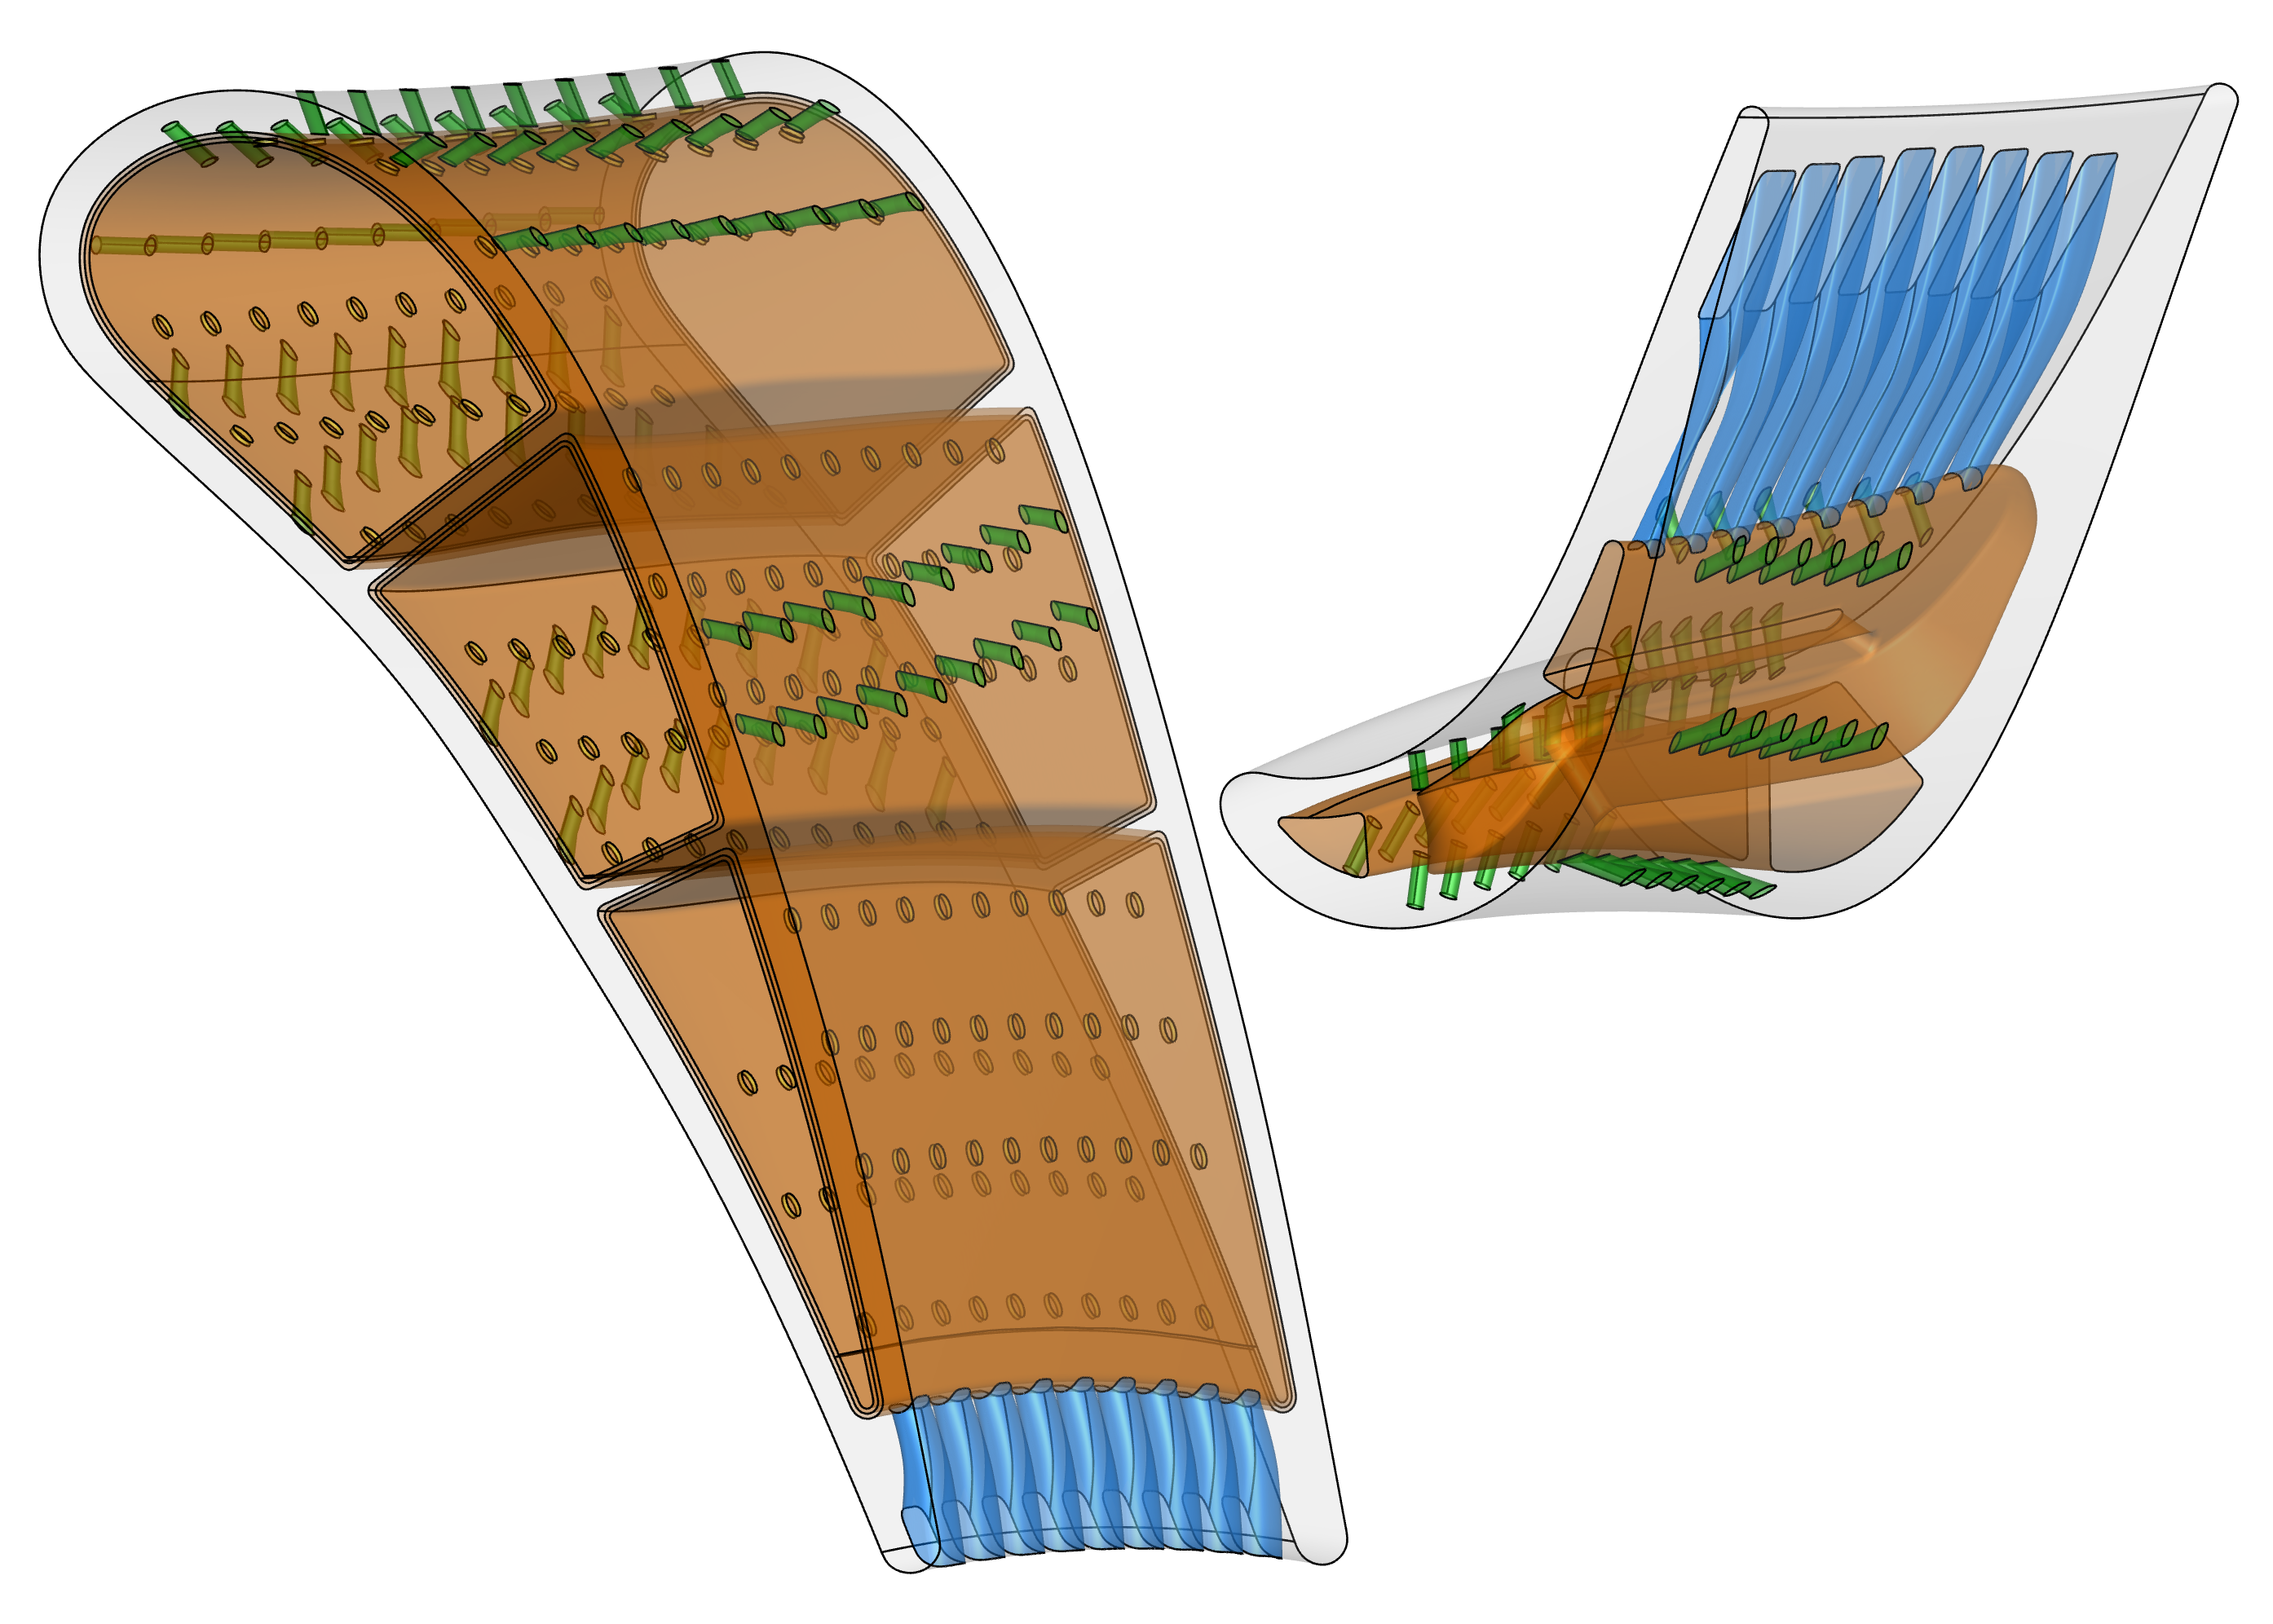
\includegraphics[width=\textwidth]{../tec/complete/title.png}
		\end{minipage}\\[\titlefigurespace]
		\begin{minipage}{.6\textwidth}
			\centering
				\today\\
				Julian Lüken\\
				\texttt{julian.lueken@dlr.de}
		\end{minipage}\\[\largetitlespace]
		\begin{minipage}{.5\textwidth}
			\centering
			Institute for Numerical and Applied Mathematics\\at the Georg-August-University Göttingen\\[\titlespace]
			Institute for Propulsion Technology\\at the German Aerospace Center in Göttingen\\[\titlespace]
			Bachelor's and master's theses\\at the Center for Computational Sciences\\at the Georg-August-University Göttingen\\[\titlespace]
		\end{minipage}\\[\largetitlespace]
		\begin{minipage}{\textwidth}
			\centering
			\begin{minipage}{.32\textwidth}
				\flushright
				First examiner: \\
				Second examiner: \\
				Advised by:
			\end{minipage}
			\hspace{0.5em}
			\begin{minipage}{.45\textwidth}
				\flushleft
				Prof. Dr. Gerlind Plonka-Hoch\\
				Prof. Dr. Christoph Lehrenfeld\\
				M.Sc. Robin Schöffler
			\end{minipage}
		\end{minipage}
	\end{center}
\end{titlepage}
\pagebreak

% Address page
\pagestyle{empty}
\restoregeometry
\newgeometry{top=210mm, left=45mm, right=45mm}
\noindent
\begin{tabular}{l}
Georg-August-University Göttingen\\
Institute of Computer Science\\
\end{tabular}\\[1em]
\begin{tabular}{ll}
	\Telefon 	&+49 (551) 39-172000\\
	\FAX 		&+49 (551) 39-14403\\
	\Letter 	&\texttt{office@cs.uni-goettingen.de}\\
\end{tabular}\\[1em]
\begin{tabular}{l}
\texttt{www.informatik.uni-goettingen.de}\\
\end{tabular}\\[1em]
\pagebreak

% Done-it-myself page
\noindent I hereby declare that this thesis has been written by myself and no other resources than those mentioned have been used.\\[0.7em]
\phantom{H}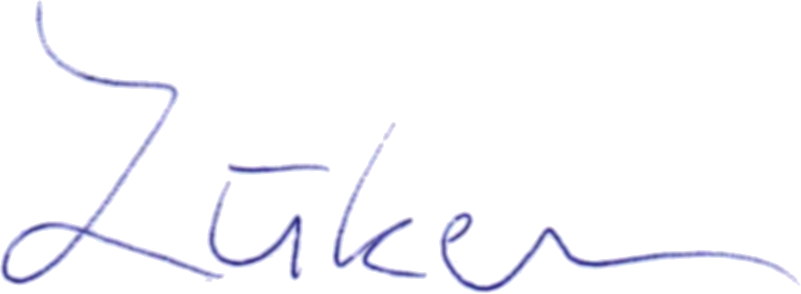
\includegraphics[height=3em]{../assets/formal/sign.png}\\[0.5em]
Göttingen, \today \hspace{2em}
\pagebreak

% Abstract and Zusammenfassung
\restoregeometry
\newgeometry{top=40mm, left=35mm, right=35mm}
\thispagestyle{plain}
\pagenumbering{roman}
\setcounter{page}{3}
\abstract{
	\lipsum[1]
}
\vspace{2cm}
\zusammenfassung{
	\lipsum[3]
}
\pagebreak

% Table of contents
\restoregeometry
\tableofcontents
\pagebreak

% Actual document starts here
\restoregeometry
\pagenumbering{arabic}
\setcounter{page}{1}
\pagestyle{plain}

\chapter{Introduction}
	Modelling cooling geometries inside of existing turbine blades and vanes using conventional interactive computer-aided design (CAD) methods currently is a difficult but necessary process in the design of modern jet engine turbines. For this purpose, the German Aerospace Center (DLR, Deutsches Zentrum für Luft- und Raumfahrt) has been concerned with finding a simple method to model cooling structures. As part of many CAD-related research projects at the DLR, parametric CAD has proven to be a simpler alternative to its conventional counterpart. The complexity and inevitable inter-dependence of cooling structures has ever since been a challenge in the development of a parametric CAD tool made solely for turbine cooling. In this thesis, we present CoolingGen, a high-performance tool that uses custom-made algorithms and evidently satisfies the goal of creating models of such cooling structures.

	% Prozesskette?
	\section{Cooling Design}
		\begin{figure}[H]
			\centering
			\includesvg[width=.6\textwidth]{../assets/turbofan}
			\caption{Schematic diagram illustrating the operation of a 2-spool, low-bypass turbofan jet engine, with low pressure spool in green and high pressure spool in purple. Credit: K. Aainsqatsi.}
		\end{figure}

		In a jet engine, kinetic energy is supplied from high pressure gas combustion. To increase the jet engine's thermodynamic efficiency, the firing temperature of the combustion chamber must be increased. In modern jet engine turbines, the hot gas temperature after combustion exceeds the materials' thermal limits. To combat this extreme condition, 20\% to 30\% of the compressed air that precedes the combustion chamber is used as a coolant, which is passed through the blades and vanes of the high pressure turbine. Alongside material selection and treatment of the coolant, the design of cooling measures includes the creation of sensible cooling geometries that are located within the blade or vane (see \cite{Giampaolo2020}, Section 4.2.1).

	\section{State of the Art}
		Conventional CAD systems are modelers that allow their user to create free-form curves and surfaces using interactive control points that can be moved to any location on a three-dimensional canvas. This gives the user an unlimited amount of strategies for creating a CAD model fit for their use. However, the amount of possible modelling strategies impedes the adaptability of most resulting models. An alternative to conventional CAD systems are feature-based parametric CAD systems, which rely on a parent-child structure of a model and its constituent parts (see \cite{Shah1995} and \cite{Camba2016}). In parametric CAD software, the user specifies a select set of (non-)geometric parameters that determine the shape of the output geometry. The number of input parameters determines the flexibility of the shape of an output model. A high number of parameters generally improves flexibility, although keeping this number as low as possible ensures simple user interaction. As Albert Einstein once famously said: "everything should be made as simple as possible, but not simpler". 

		Because of it's intrinsic adaptability, feature-based CAD has become an important and widely used tool among many mechanical engineering applications. To adapt the geometry of a mechanical model in parametric CAD, as opposed to conventional CAD, the user simply has to change a few parameters instead of moving control points, which in themselves bear no underlying semantic structure regarding their mechanical function.

		Using conventional interactive CAD software, the creation of cooling geometries is labour-intensive and requires expertise. The approach of automating this process using a set of parameters certainly bears great potential in this regard. At the DLR, blade and vane contours are already successfully designed using a parametric CAD in a tool called BladeGen. In the associative structure of parametric CAD, blades and vanes serve as the parent element of the cooling geometries we are concerned with in the development of CoolingGen.

	\section{Problem Statement}
		CoolingGen is a parametric CAD software written in the programming language C that allows for the creation of three-dimensional turbine cooling geometries of blades and vanes. It was first developed by Timo Schumacher and Christian Voß in 2013 at the DLR. The 2013 release, while being a great proof of concept, lacked an underlying framework of established geometric methods and thus failed to fulfill real world requirements. It was tailored to fit only a few parameter configurations on a certain parent blade surface. In 2022, CoolingGen was largely revised as part of this thesis to support realistic cooling geometries.

		Currently, CoolingGen supports four distinct types of cooling geometries: internal cooling, film cooling, impingement cooling and ejection slots. The internal cooling is comprised of cooling channels, which are hollow sections inside a turbine blade or vane. They allow for a coolant to pass through. The film cooling consists of holes that transfer the coolant from the inside of a channel to the outside of the blade or vane. An array of these holes provides a protective fluid layer that restrains net heat transfer to the blade or vane. Impingement inserts are thin sheets that reside within channels and have cylindrical holes in them. The ejection slots are hollow bodies that transports the coolant from the inside of the trailing edge channel to the trailing edge or pressure side of the turbine blade or vane.

		The parameters for each of these cooling geometries are provided in the Extensible Markup Language (XML). The geometries are modeled using Non-Uniform Rational B-spline (NURBS) surfaces. To create a complete set of cooling geometries for a single blade or vane, CoolingGen currently averages out at approximately 20 seconds on a modern home computer.
		
		This thesis essentially highlights the geometric methods that are imperative to achieve CoolingGen's goals in terms of accuracy and speed in Chapter 2. The fundamental methods of jet engine design required for channel creation are presented in Chapter 3. Combining the methods from Chapter 2 and Chapter 3, we are able to create all aforementioned cooling geometries. Their exact construction is explained and illustrated using examples in Chapter 4.

\chapter{Geometric Methods}\label{chap:methods}
	As stated before, NURBS curves and surfaces are used to model geometries in CoolingGen. In this chapter we will first introduce Bézier curves. We will then generalize Bézier curves to obtain B-spline curves and surfaces. Applying an embedding map and a projection map to B-spline curves and surfaces, we acquire NURBS curves and surfaces, which are a generalization of B-spline curves and surfaces. Furthermore, CoolingGen uses special geometric algorithms such as point projection, ray marching, curve intersection, offset curve creation and fillet creation, which we will also present.

\section{Bézier Curves}
	Bézier curves are named after the French engineer Pierre Bézier, who famously utilized them in the 1960s to design car bodies for the automobile manufacturer Renault \cite{Bezier1968}. Today, they are used in a wide variety of vector graphics applications (i.e. in font representation on computers). At first glance, the definition of the Bézier curve might seem cumbersome, but given the mathematical foundation and a few graphical representations, it becomes apparent why they are such a powerful tool in CAD. In this section, we present the famous algorithm of de Casteljau and some important properties of Bézier curves according to \cite{Farin2001}.

	\begin{figure}[H]
		\centering
		\begin{subfigure}{0.25\textwidth}
			\includesvg[width=\textwidth]{../python/bezierDifferentDegrees1}
			\caption{Degree $1$.}
		\end{subfigure}
		\begin{subfigure}{0.25\textwidth}
			\includesvg[width=\textwidth]{../python/bezierDifferentDegrees2}
			\caption{Degree $2$.}
		\end{subfigure}
		\begin{subfigure}{0.25\textwidth}
			\includesvg[width=\textwidth]{../python/bezierDifferentDegrees3}
			\caption{Degree $3$.}
		\end{subfigure}
		\caption{Bézier curves of different degrees (orange) and their control points (blue).}
		\label{fig:bezierdifferentdegrees}
	\end{figure}

\subsection{Definition}
	\begin{definition}
		The \emph{Bernstein basis polynomials} of degree $n$ on the interval $[t_0,t_1]$ are defined as
		\begin{equation}\label{eq:bernsteinbasisdef}
			b_{n,k,[t_0, t_1]}(t) := \frac{\binom{n}{k} (t_1-t)^{n-k}(t-t_0)^k}{(t_1-t_0)^n},
		\end{equation}
		for $k \in \{0,\dots, n\}$.
	\end{definition}

	\begin{definition}
		A \emph{Bézier curve} of degree $n$ is a parametric curve $B_{P,[t_0, t_1]}: [t_0, t_1] \rightarrow \mathbb{R}^d$ that has a representation
		\begin{equation}\label{eq:bezierdef}
			B_{P, [t_0, t_1]}(t) = \sum_{k=0}^n b_{n,k,[t_0, t_1]}(t) P_k = \sum_{k=0}^n \frac{\binom{n}{k} (t_1-t)^{n-k}(t-t_0)^k}{(t_1-t_0)^n} P_k.
		\end{equation}
		We call the elements of the set $P = \{P_0, P_1, \dots, P_n\} \subset \mathbb{R}^d$ the \emph{control points} of $B_P$.
	\end{definition}

	\begin{remark}
		Let $t_0 = 0$ and $t_1 = 1$. Then Equation (\ref{eq:bezierdef}) simplifies to
		\begin{equation*}
			b_{n,k}(t) := b_{n,k,[0,1]}(t) = \binom{n}{k} (1-t)^{n-k}t^k
		\end{equation*}
		and Equation (\ref{eq:bernsteinbasisdef}) simplifies to
		\begin{equation}\label{eq:bezierdefshort}
			B_P(t) := B_{P,[0,1]}(t)= \sum_{k=0}^n \binom{n}{k} (1-t)^{n-k}t^k P_k.
		\end{equation}
		This case is the only case considered in this thesis.
	\end{remark}

	In a Bézier curve of a given degree, the control points completely determine the shape of the curve. This behavior can be observed in Figure \ref{fig:bezierdifferentdegrees}. However, changing one control point affects the whole curve, since for $n$ control points the degree of the Bézier curve is always $n-1$. This behavior also becomes apparent using de Casteljau's algorithm for the computation of points on the Bézier curve.

\subsection{De Casteljau's Algorithm}
	The computation of Equation (\ref{eq:bezierdefshort}) is usually performed using de Casteljau's algorithm. This is because the algorithm yields a simple implementation and lower complexity than straightforwardly computing Equation (\ref{eq:bezierdefshort}). The algorithm was proposed by Paul de Faget de Casteljau for the automobile manufacturer Citroën in the 1960s.

	\begin{algorithm}[H]
		\begin{algorithmic}[1]
			\Input
				\Desc{$P = \{P_0, P_1, ..., P_n\}$}{set of control points}
				\Desc{$t$}{real number}
			\EndInput
			\Output
				\Desc{$P^{(n)}_0 = B_P(t)$}{the point on the Bézier curve w.r.t. to $t$}
			\EndOutput

			\caption{de Casteljau's algorithm}\label{alg:decasteljaualgo}
			\Procedure{deCasteljau}{$P, t$}
				\State $P^{(0)} \gets P$
				\For {$j = 1, 2, ..., n$}
					\For {$k = 0, 1, ..., n-j$}
						\State $P^{(j)}_k \gets (1-t) \cdot P^{(j-1)}_k + t \cdot P^{(j-1)}_{k+1}$
					\EndFor
				\EndFor
				\State \Return $P^{(n)}_0$
			\EndProcedure
		\end{algorithmic}
	\end{algorithm}

	\begin{theorem}
		Algorithm \ref{alg:decasteljaualgo} computes $B_P(t)$.
	\end{theorem}
	\begin{proof}
		By induction. Let $n = 1$ and $t \in [0,1]$ be fixed. Then
			$$ P_0^{(1)} = (1-t) \cdot P_0 + t \cdot P_1.$$
		By employing the induction hypothesis
			$$ P_j^{(n)} = \sum_{k=j}^{n+j} \binom{n}{k} (1-t)^{n-k}t^k P_{j+k}$$
		for some $n \in \mathbb{N}$, we can infer that
		\begin{align*}
			P_0^{(n+1)}	&= (1-t) \cdot P_0^{(n)} + t \cdot P_1^{(n)} \\
						&= (1-t) \cdot \sum_{k=0}^{n} \binom{n}{k} (1-t)^{n-k}t^k P_{k} + t \cdot \sum_{k=1}^{n+1} \binom{n}{k} (1-t)^{n-k}t^k P_{k+1} \\
						&= \sum_{k=0}^{n+1} \binom{n+1}{k} (1-t)^{n+1-k}t^k P_{k},
		\end{align*}
		which is equal to $B_P(t)$ for degree $n+1$.
	\end{proof}

	A visual representation of Algorithm \ref{alg:decasteljaualgo} yields a triangular scheme. To compute one point on a Bézier curve $B_P$ with degree $n$, one has to perform $\frac{n^2-n}{2}$ vector additions and $n^2-n$ scalar multiplications.

	\begin{figure}[H]
		\centering
		\begin{subfigure}{0.49\textwidth}
			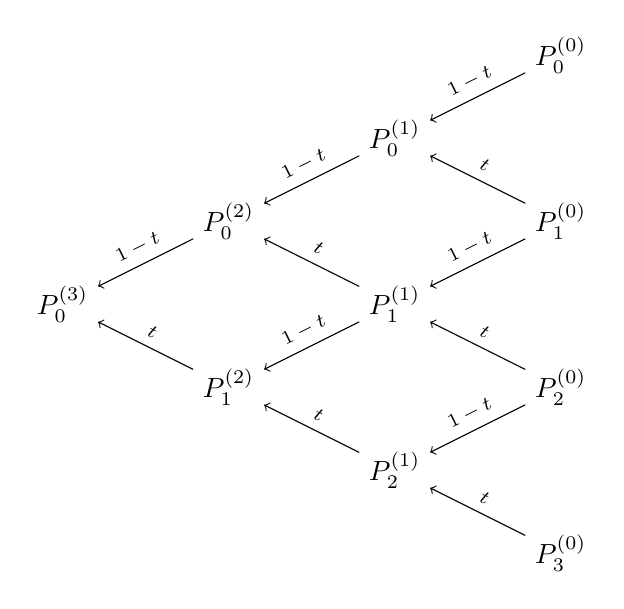
\begin{tikzpicture}
				\def\dx{60pt}
				\def\dy{30pt}

				\pgfmathsetmacro{\degree}{3}

				% Make nodes
				\newcounter{i}
				\newcounter{j}

				\node (\arabic{i}) at (0,0) {$P^{(\degree)}_0$};
				\stepcounter{i}

				\foreach \x in {1, ..., \degree} {
					\pgfmathsetmacro{\xstep}{\x-2}

					\setcounter{j}{0}
					\foreach \y in {\x, \xstep, ..., -\x} {
						\node (\arabic{i}) at (\x*\dx, \y*\dy) {$P^{(\pgfmathint{\degree-\x}\pgfmathresult)}_{\arabic{j}}$};
						\stepcounter{i}
						\stepcounter{j}
					}
				}
				
				% Make arrows
				\newcounter{z}
				\newcounter{a}
				\newcounter{b}
				\pgfmathsetmacro{\maxx}{\degree}
				\foreach \x in {1,...,\degree}{
					\foreach \y in {1,...,\x}{
						
						\setcounter{a}{\arabic{z}}
						\addtocounter{a}{\x}

						\setcounter{b}{\arabic{z}}
						\addtocounter{b}{\x}
						\stepcounter{b}
						
						\draw [<-] (\arabic{z}) -- (\arabic{a}) node[above, midway, sloped] {\scriptsize $1-t$};
						\draw [<-] (\arabic{z}) -- (\arabic{b}) node[above, midway, sloped] {\scriptsize $t$};
						
						\stepcounter{z}
					}
				}
			\end{tikzpicture}
			\caption{Algorithmic visualization.}
		\end{subfigure}
		\hfill
		\begin{subfigure}{0.49\textwidth}
			\includesvg[width=\textwidth]{../python/deCasteljauVisual}
			\caption{Geometric visualization of $B_P(\frac{3}{5})$.}
		\end{subfigure}
		\caption{Visual representations of de Casteljau's algorithm.}
		\label{fig:decasteljautriangle}
	\end{figure}

	Interestingly, the representation of the algorithm in Figure \ref{fig:decasteljautriangle} also gives rise to an intuitive visualization of the geometric shape of the Bézier curve $B_P$. For all $i \in \{0, ..., n\}$ and all $j \in \{0, ..., n-i\}$, the point $P^{(i+1)}_j$ is the convex combination (always w.r.t. $t$) of $P^{(i)}_j$ and $P^{(i)}_{j+1}$. Thus $P^{(i+1)}_j$ always lies on the line segment between $P^{(i)}_j$ and $P^{(i)}_{j+1}$, as can be observed in the example in Figure \ref{fig:decasteljautriangle}.

\subsection{Properties}
	Other than being remarkably intuitive, Bézier curves have a lot of covenient properties. In CAD software, most graphical user interfaces rely on the principle of letting the user interactively drag and drop the control points with a mouse, granting them control over the shape of the whole Bézier curve. The following theorems further illustrate why this is a good concept.

	\begin{theorem}\label{thm:bezierendpoints}
		We have $B_P(0) = P_0$ and $B_P(1) = P_n$.
	\end{theorem}
	\begin{proof}
		Explicit computation for $t=0$ and $t=1$ yields
			$$B_P(0) = \sum_{k=0}^n \binom{n}{k} t^k P_k = \binom{n}{0} P_0 = P_0$$
		and
			$$B_P(1) = \sum_{k=0}^n \binom{n}{k} (1-t)^{n-k} P_k = \binom{n}{n} P_n = P_n.$$
	\end{proof}

	\begin{theorem}\label{thm:bezieraffinetransform}
		Let $T \in \mathbb{R}^{3 \times 3}$. Then $B_{TP}(t) = TB_P(t)$ where $TP := \{TP_0, TP_1, ..., TP_n\}$.
	\end{theorem}
	\begin{proof}
		For all $t \in [0, 1]$ we can directly compute
			$$TB_P(t) = \sum_{k=0}^n \binom{n}{k} (1-t)^{n-k}t^k TP_k = B_{TP}(t).$$
		This property is called invariance with respect to linear transforms.
	\end{proof}

	\begin{theorem}\label{thm:bezierconvexhull}
		The Bézier curve $B_P(t)$ lies in the convex hull of $P$ for all $t \in [0,1]$.
	\end{theorem}
	\begin{proof}
		By the algorithm of de Casteljau (\ref{alg:decasteljaualgo}), we know that $P^{(i)}_j = (1-t) \cdot P^{(i-1)}_j + t \cdot P^{(i-1)}_{j+1}$ for all $t \in [0, 1]$. Therefore, $P^{(i)}$ lie in the convex hull of $P^{(i-1)}$. But then $B_P(t) = P^{(n)}_0$ always lies in the convex hull of $P^{(0)} = P$ by induction.
	\end{proof}

	Theorem \ref{thm:bezierendpoints} guarantees the control over the end points of the the curve, whereas Theorem \ref{thm:bezierconvexhull} ensures that the Bézier curve lies close to the control points. Theorem \ref{thm:bezieraffinetransform} shows that transformations such as rotations and projections can be applied directly to the control points instead of the points on the curve.

	Simple as their appearance may be, Bézier curves fall short of representing some of the most common geometric shapes. Given a finite number of control points, we can never make $B_P(t)$ a circular arc, although a circle has a very simple parametric form. One of their greatest perks, the ability to describe a shape with a low number of of control points, is simultaneously one of their greatest shortcoming. This is most likely the reason why Bézier curves are not the state of the art in technical engineering applications. However, Bézier curves certainly do provide an intuition for NURBS, which is their prevailing counterpart.

\section{Non-Uniform Rational B-splines (NURBS)}
	NURBS are another tool for curve and surface modelling. There is a somewhat common joke that describes the acronym NURBS as \emph{"Nobody Understands Rational B-Splines"}, which can be found at the back of \cite{Piegl1997}. In this section, we invalidate this punch line. First of all, we discuss B-splines and construct B-spline curves and surfaces according to \cite{Farin2001}, including the famous algorithm of de Boor. Then we apply simple transformations to the B-spline curves and surfaces to acquire NURBS curves and surfaces as described in \cite{Piegl1997}.

\subsection{Definition}
	Similarly to how Bézier curves are defined on the Bernstein polynomial basis, NURBS are defined on basis functions called basis splines or, more commonly, B-splines.

	\begin{definition}
		A \emph{knot sequence} $(t_m)_{m=-\infty}^{\infty} \subset \mathbb{R}$ is a sequence with $t_{m} \leq t_{m+1}$ for all $m \in \mathbb{Z}$.
	\end{definition}

	\begin{definition}
		The \emph{B-splines of degree $0$} on a knot sequence $(t_m)$ are defined as
		\begin{equation}
			N^{(t_m)}_{1,k}(t) :=
			\begin{cases}
				1 & \text{if } t \in [t_k, t_{k+1}),\\
				0 & \text{else.}
			\end{cases}
		\end{equation}
		The \emph{B-splines of degree $p-1$} with $p > 1$ are given by the \emph{Cox-de-Boor recursion formula}
		\begin{equation}\label{eq:coxdeboorrec}
			N_{p,k}^{(t_m)}(t) := \omega^{(t_m)}_{p-1, k}(t) \, N^{(t_m)}_{p-1, k}(t) + (1-\omega^{(t_m)}_{p-1, k+1}(t)) \, N^{(t_m)}_{p-1, k+1}(t),
		\end{equation}
		where
		\begin{equation}
			\omega^{(t_m)}_{p,k}(t) := 
			\begin{cases}
				\frac{t-t_k}{t_{k+p} - t_k} &\text{if } t_{k+p} \neq t,\\
				0 							&\text{else.}
			\end{cases}
		\end{equation}
	\end{definition}

	\begin{remark}
		Instead of $N_{p,k}^{(t_m)}$ we write $N_{p,k}$ and explicitly refer to $(t_m)$ when necessary. We restrict the domain of definition of $N_{p,k}$ to $[0, 1]$ by setting $\lim_{m \to -\infty} t_m = 0$ and $\lim_{m \to \infty} t_m = 1$.
	\end{remark}

	\begin{definition}
		A \emph{B-spline curve} of degree $p-1$ over a set of control points
			$$P = \{P_0, P_1, ... P_n\} \subset \mathbb{R}^d$$
		and a knot sequence $(t_m)$ is defined as
			$$ S_P(t) = \sum_{k=0}^{n} N_{p,k}(t) P_k.$$
	\end{definition}

	\begin{definition}\label{def:nurbs}
		A \emph{NURBS curve} $C_P(t)$ of degree $p-1$ with the control points 
			$$P = \{P_0, P_1, ..., P_n\} \subset \mathbb{R}^d,$$ 
		the control weights $w = (w_0, w_1, ... w_n) \subset \mathbb{R}$ and a knot sequence $(t_m)$ is defined as
		\begin{equation}
			C_P(t) = \frac{\sum_{k=0}^n N_{p,k}(t) w_k P_k}{\sum_{k=0}^n N_{p,k}(t) w_k}.
		\end{equation}
	\end{definition}

	\begin{remark}
		Let $P \subset \mathbb{R}^d$. A NURBS curve can alternatively be understood as a projection of a B-spline curve on a transformed set of control points. For this purpose we define the embedding into the weighted vector space
			$$\Phi_w: \mathbb{R}^d \rightarrow \mathbb{R}^{d+1}$$
		that maps each control point $P_k = (p_1, ..., p_d) \in \mathbb{R}^d$ onto $(w_k p_1, ..., w_k p_d, w_k) \in \mathbb{R}^{d+1}$.
		We also have to define the projection map
			$$\Phi^\dagger: \mathbb{R}^{d+1} \rightarrow \mathbb{R}^d$$ 
		that maps each point on the B-spline curve $S_{\Phi(P)}(t) = (s_1, ..., s_d, s_{d+1})$ onto $(\frac{s_1}{s_{d+1}}, ..., \frac{s_d}{s_{d+1}})$.
		We can then define the NURBS curve as
				$$ C_P(t) = \Phi^\dagger(S_{\Phi_w(P)}(t)).$$ 
	\end{remark}

	Utilizing the notation with the embedding map $\Phi_w$ and the projection map $\Phi^\dagger$, we will calculate points on an arbitrary NURBS curve by calculating points on a corresponding B-spline curve. To do this, we employ the following steps on a set of control points $P$ and the weights $w$:
	\begin{enumerate}
		\item Calculate $P_w = \Phi_w(P)$.
		\item Calculate points on $S_{P_w}$.
		\item Project points onto $\mathbb{R}^d$ by applying $\Phi^\dagger$ to $S_{P_w}$ to find $C_P$.
	\end{enumerate}
	The calculation of points on a B-spline curve can be done similarly to the calculation of a point on a Bézier curve. The exact method is presented in the next section.

	\begin{theorem}
		Let $w \equiv 1$. Then $S_P \equiv \Phi^\dagger(S_{\Phi_w(P)})$. In other words, NURBS curves are a generalization of B-spline curves.
	\end{theorem}
	\begin{proof}
		Since in this case $\Phi_w((p_1, ..., p_d)) = (p_1, ..., p_d, 1)$, we have
			$$\Phi^\dagger(S_{\Phi_w(P)}(t)) = \Phi^\dagger(\Phi_w(S_P(t))) = S_P(t).$$
	\end{proof}

	\begin{figure}[H]
		\centering
		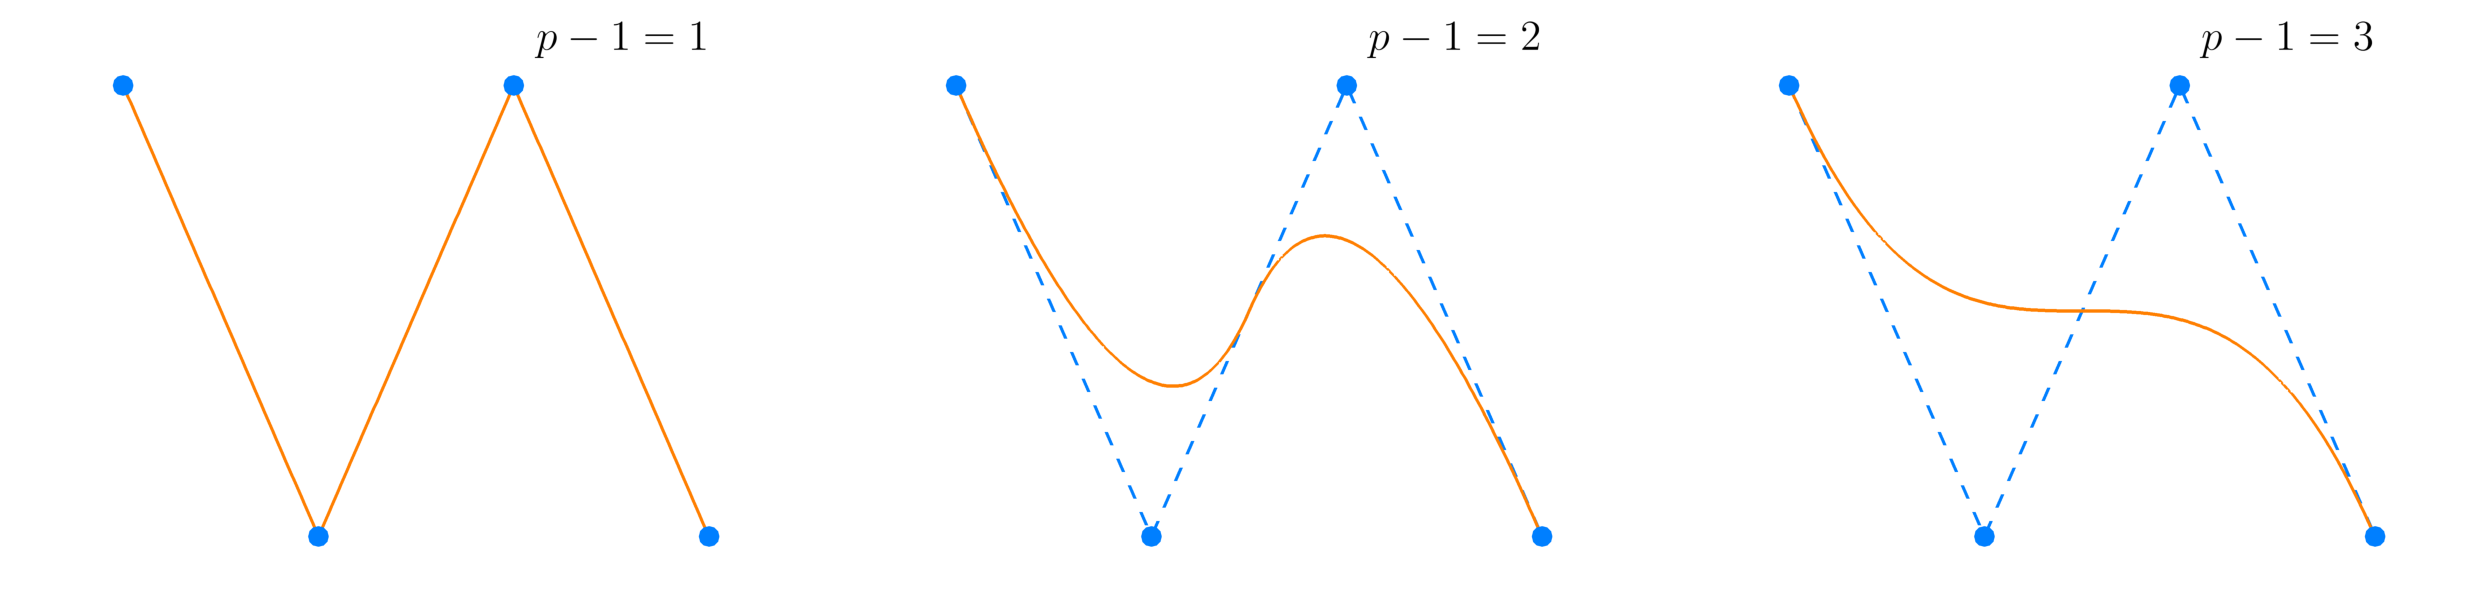
\includegraphics[width=\textwidth]{../tec/nurbsCurve/nurbsCurve.png}
		\caption{A set of control points and three NURBS curves of different degrees.}
	\end{figure}

	Now that we have defined B-spline curves and NURBS curves, we can define B-spline surfaces and NURBS surfaces in a similar manner. To do this, we require a grid of knots represented by two knot sequences $(u_m)_{m=-\infty}^{\infty}$ and $(v_m)_{m=-\infty}^{\infty}$ which satisfy the same conditions as $(t_m)$ did before. Instead of a one-dimensional set of control points, the surface definition relies on a two-dimensional set of control points.

	\begin{definition}
		A \emph{B-spline surface} $S_P(u,v)$ of degree $(p-1, q-1)$ over a set of control points $P = \{P_{i,j} : (i,j) \in \{0,1,...,n_u\} \times \{0,1,...,n_v\}\} \subset \mathbb{R}^d$ on the knot grid $(u_m), (v_m)$ is defined as
			$$ S_P(u,v) = \sum_{k_u=0}^{n_u} \sum_{k_v=0}^{n_v} N_{p,k_u}(u) N_{q,k_v}(v) P_{k_u,k_v},$$
		where $N_{p,k_u}(u) := N_{p,k_u}^{(u_m)}(u)$ and $N_{q,k_v}(v) := N_{q,k_v}^{(v_m)}(v)$.
	\end{definition}

	\begin{definition}
		A \emph{NURBS surface} $C_P(u,v)$ of degree $(p-1, q-1)$ over a set of control points $P = \{P_{i,j} : (i,j) \in \{0,1,...,n_u\} \times \{0,1,...,n_v\}\} \subset \mathbb{R}^d$, the control weights $w = \{w_{i,j} : (i,j) \in \{0,1,...,n_u\} \times \{0,1,...,n_v\}\} \subset \mathbb{R}$ and the knot grid $(u_m), (v_m)$ is defined as
			$$ C_P(u,v) = \frac {\sum_{k_u=0}^{n_u} \sum_{k_v=0}^{n_v} N_{p,k_u}(u) N_{q,k_v}(v) w_{k_u, k_v} P_{k_u,k_v}}{\sum_{k_u=0}^{n_u} \sum_{k_v=0}^{n_v} N_{p,k_u}(u) N_{q,k_v}(v) w_{k_u, k_v}},$$
		where $N_{p,k_u}(u) := N_{p,k_u}^{(u_m)}(u)$ and $N_{q,k_v}(v) := N_{q,k_v}^{(v_m)}(v)$.
	\end{definition}

	\begin{remark}
		As with NURBS curve, we have the analogous result
			$$ C_P(u,v) = \Phi^\dagger ({S_{\Phi_w(P)}(u,v)}) $$
		for NURBS surfaces, which also yields the same calculation strategy.
	\end{remark}

	\begin{figure}[H]
		\centering
		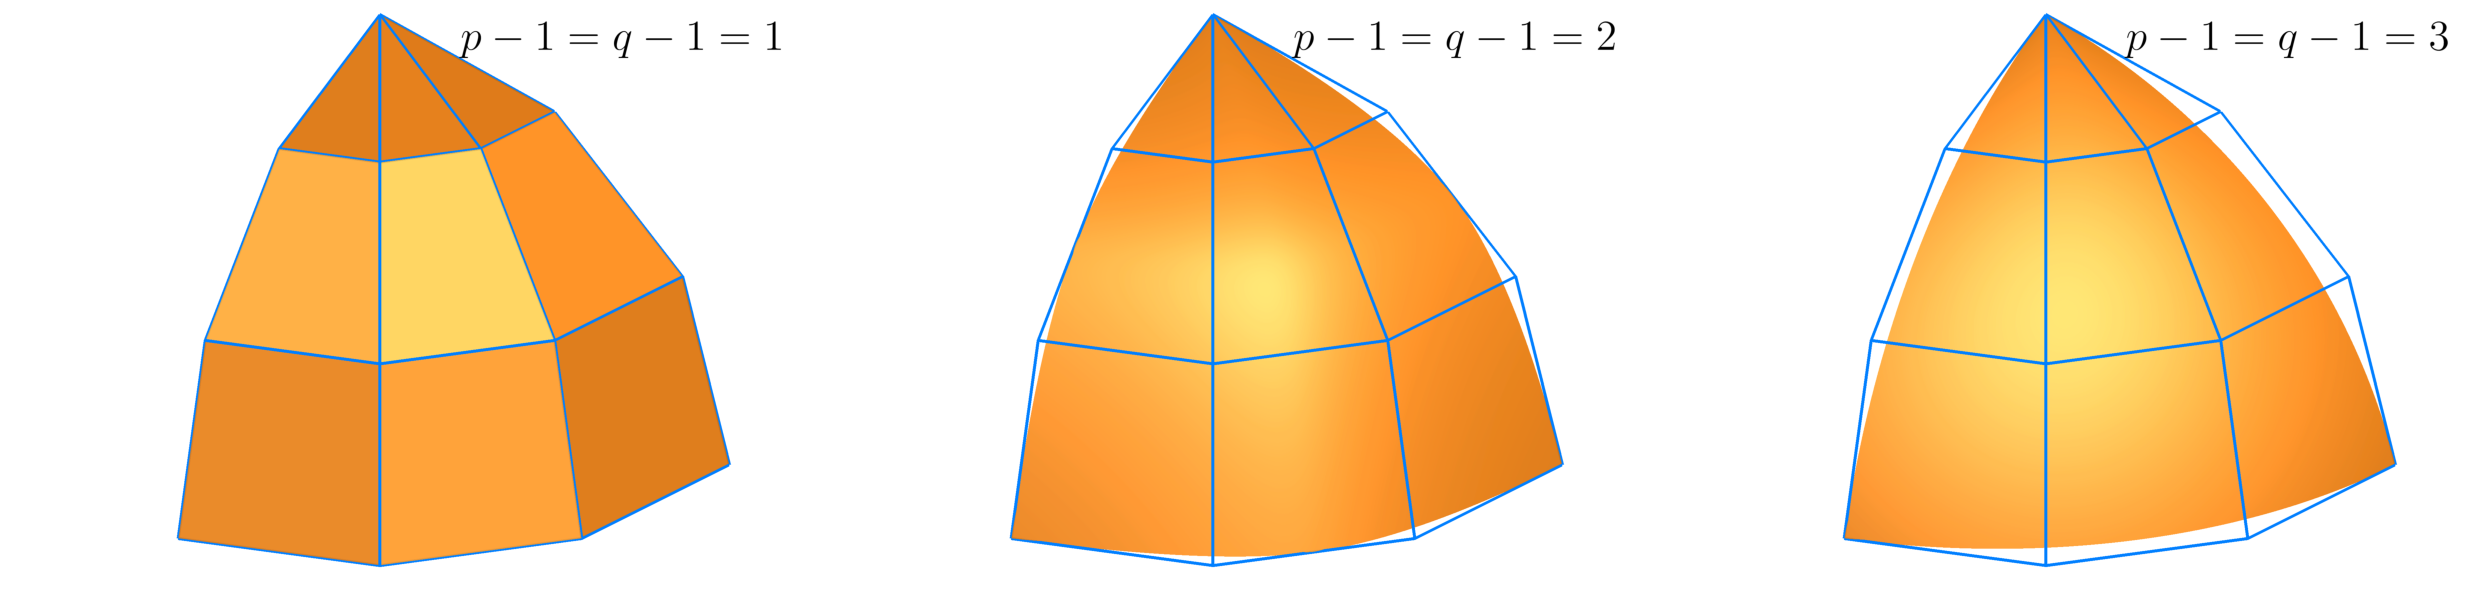
\includegraphics[width=\textwidth]{../tec/nurbsSurface/nurbsSurface.png}
		\caption{A set of control points and three NURBS surfaces of different degrees.}
	\end{figure}

	The notion of the knot sequence $(t_m)$ is commonly computationally simplified to that of a knot vector $\tau$, since $\tau$ only contains a finite number of elements. For our purposes, we let
		$$\tau = (\underbrace {t_0, ..., t_{p-1}}_{= 0}, t_p, ..., t_n, \underbrace{t_{n+1}, ..., t_{n+p}}_{= 1}),$$
	where $t_k = 0$ for $k \in \{0,...,p-1\}$ and $t_k = 1$ for $k \in \{n+1, ..., n+p\}$. We still require the monotonicity property $t_k \leq t_{k+1}$ for all $k \in \{0, ..., n+p\}$.

\subsection{De Boor's Algorithm}
	To efficiently calculate points on a B-spline object, Carl-Wilhelm Reinhold de Boor devised an efficient algorithm, the construction of which demonstrates its correctness. Together with the embedding $\Phi_w$ and the projection $\Phi^\dagger$ from the Remark for Definition \ref{def:nurbs}, this algorithm can also be used to calculate points on a NURBS object.

	Let $P = \{P_0, P_1, ..., P_n\}$ be a set of control points, $(t_m)$ a knot sequence and $p-1$ the degree of the B-spline curve $S(t)$. Then by the Cox-de-Boor recursion formula, we find
	\begin{align*}
		S(t) 	&= \sum_{k=0}^n N_{p,k}(t) \, P_k \\
				&= \sum_{k=1}^n \omega_{p-1,k}(t) \, N_{p-1, k}(t) \, P_k  \; + \; \sum_{k=0}^n \left( 1-\omega_{p-1,k+1}(t) \right) \, N_{p-1, k+1}(t) \, P_k.
	\end{align*}
	Shifting the summation index in the second sum, we can summarize the two sums0 as
	\begin{align*} 
		S(t) 	&= \sum_{k=1}^n N_{p-1, k}(t) \, \underbrace{\Big[ \omega_{p-1,k}(t) \, P_k  \, + \, \left( 1-\omega_{p-1,k}(t) \right) \, P_{k-1} \Big]}_{=: P_k^{(1)}(t)} \\
				&= \sum_{k=1}^n N_{p-1, k}(t) \, P_k^{(1)}(t).
	\end{align*}
	Recursively defining
	\begin{equation}\label{eq:debooriteration}
		P^{(j)}_k(t) := \begin{cases}
			\omega_{p-j, k} \, P^{(j-1)}_k(t) \, + \, (1-\omega_{p-j, k}) \, P^{(j-1)}_{k-1}(t) 	&\text{if } j > 0,\\
			P_k 																					&\text{else},
		\end{cases}
	\end{equation}
	we can repeat this process up to $p-2$ more times, finding
	$$ S(t) = \sum_{k=p-1}^n N_{1, k}(t) \, P^{(p-1)}_k(t) = P^{(p-1)}_l(t)$$
	for $t \in [t_l, t_{l+1})$. We can thus use the recursive definition in Equation (\ref{eq:debooriteration}) as the key step of our algorithm to compute $S(t)$. It becomes apparent that the points calculated on a B-spline curve are in fact also a cumultated convex combination of control points, just as it is the case with Bézier curves. As zero-values for $\omega_{i,j}$ (or $1-\omega_{i,j}$) can be completely omitted by counting how often the $t$ occurs in the knot vector, we arrive at the following algorithm:

	\begin{algorithm}[H]
		\begin{algorithmic}[1]
			\Input
				\Desc{$P = \{P_0, P_1, ..., P_n\}$}{set of control points of the B-spline curve}
				\Desc{$\tau = (t_0, t_1, ..., t_{n+p})$}{knot vector of the B-spline curve}
				\Desc{$p-1$}{degree of the B-spline curve}
				\Desc{$t \in [t_0, t_{n+p})$}{real number}
			\EndInput
			\Output
				\Desc{$S_P(t)$}{the point on the B-spline curve w.r.t. to $t$}
			\EndOutput

			\caption{de Boor's algorithm for curves}\label{alg:debooralgo}
			\Procedure{deBoorCurve}{$P, p, \tau, t$}
				\State Find $l$ such that $t \in [t_l, t_{l+1})$
				\State Let $m$ be the multiplicity of $t$ in the knot vector $\tau$
				\State $P^{(0)} \gets P$

				\For {$j = 1, 2, ..., p-m-1$}
					\For {$k = l-p+j+1, ..., l-m$}
						\State $\omega_{p-j,k} \gets \frac{t-t_k}{t_{k+p-j} - t_k}$
						\State $P^{(j)}_k \gets (1-\omega_{p-j,k}) \cdot P^{(j-1)}_{k-1} + \omega_{p-j,k} \cdot P^{(j-1)}_k$
					\EndFor
				\EndFor

				\State \Return $P^{(p-m-1)}_{l-m} = S_P(t)$
			\EndProcedure
		\end{algorithmic}
	\end{algorithm}

	\begin{figure}[H]
		\centering
		\begin{subfigure}{0.49\textwidth}
			\begin{tikzpicture}
				\def\dx{65pt}
				\def\dy{30pt}

				\pgfmathsetmacro{\degree}{3}

				% Make nodes
				\setcounter{i}{0}
				\setcounter{j}{0}

				\node (\arabic{i}) at (0,0) {$P^{(\degree)}_l$};
				\stepcounter{i}

				\foreach \x in {1, ..., \degree} {
					\pgfmathsetmacro{\xstep}{\x-2}

					\setcounter{j}{0}
					\foreach \y in {\x, \xstep, ..., -\x} {

						\ifthenelse{\value{j}>0} {
							\node (\arabic{i}) at (\x*\dx, \y*\dy) {$P^{(\pgfmathint{\degree-\x}\pgfmathresult)}_{l-\arabic{j}}$};
						}
						{
							\node (\arabic{i}) at (\x*\dx, \y*\dy) {$P^{(\pgfmathint{\degree-\x}\pgfmathresult)}_l$};
						}
						\stepcounter{i}
						\stepcounter{j}
					}
				}
				
				% Make arrows
				\setcounter{z}{0}
				\setcounter{a}{0}
				\setcounter{b}{0}
				\pgfmathsetmacro{\maxx}{\degree}
				\foreach \x in {1,...,\degree}{
					\foreach \y in {1,...,\x}{
						
						\setcounter{a}{\arabic{z}}
						\addtocounter{a}{\x}

						\setcounter{b}{\arabic{z}}
						\addtocounter{b}{\x}
						\stepcounter{b}
						
						\ifthenelse{\y > 1} {
							\draw [<-] (\arabic{z}) -- (\arabic{b}) node[above, midway, sloped] {\scriptsize $1-\omega_{\pgfmathint{\x}\pgfmathresult, l-\pgfmathint{\y-1}\pgfmathresult}$};
							\draw [<-] (\arabic{z}) -- (\arabic{a}) node[above, midway, sloped] {\scriptsize $\omega_{\pgfmathint{\x}\pgfmathresult, l-\pgfmathint{\y-1}\pgfmathresult}$};
						}
						{
							\draw [<-] (\arabic{z}) -- (\arabic{b}) node[above, midway, sloped] {\scriptsize $1-\omega_{\pgfmathint{\x}\pgfmathresult, l}$};
							\draw [<-] (\arabic{z}) -- (\arabic{a}) node[above, midway, sloped] {\scriptsize $\omega_{\pgfmathint{\x}\pgfmathresult, l}$};
						}

						\stepcounter{z}
					}
				}
			\end{tikzpicture}
			\caption{Visualization of de Boor's algorithm on a curve $S_P(t)$ with degree $3$, where $t$ does not appear in the knot vector $\tau$ (in other words, $m=0$.}
		\end{subfigure}
		\hfill
		\begin{subfigure}{0.49\textwidth}
			\centering
			\includesvg[width=0.99\textwidth]{../python/nurbsCurveExample}
			\caption{Degree $3$ NURBS curve $\Phi^\dagger(S_{\Phi_w(P)}(t))$  for different values of a single entry of the control weight vector $w$.}
		\end{subfigure}
		\caption{Calculating points on a NURBS curve.}
		\label{fig:debooralgo}
	\end{figure}

	To calculate one point on the B-spline curve $S_P$ of degree $p$, we require at most $\frac{p^2-p}{2}$ vector additions and $p^2-p$ scalar multiplications, which is quite similar to what we found for Bézier curves. However, we also need to calculate $\omega_{j,k}$ at every step, which in total sums up to $p^2-p$ real additions and $\frac{p^2-p}{2}$ real multiplications.

	By writing the definition of the B-spline surface as
		$$ S_P(u,v) = \sum_{k_u=0}^{n_u} \sum_{k_v=0}^{n_v} N_{p,k_u}(u) N_{q,k_v}(v) P_{k_u,k_v} = \sum_{k_u=0}^{n_u} N_{p,k_u}(u) \underbrace{\left( \sum_{k_v=0}^{n_v} N_{q,k_v}(v) P_{k_u,k_v} \right)}_{:= \, q_{k_u}(v)},$$
	we can observe that Algorithm \ref{alg:debooralgo} can be utilized to calculate points on B-splines surfaces. To do this, we run the de Boor's algorithm to calculate $q_{k_u}(v)$.

	\begin{algorithm}[H]
		\begin{algorithmic}[1]
			\Input
				\Desc{$P = \{P_{i,j}\}$}{set of control points with $n_1 \cdot n_2$ elements}
				\Desc{$\tau_u = (u_0, u_1, ..., u_{n_u+p})$}{first knot vector of the B-spline curve}
				\Desc{$\tau_v = (v_0, v_1, ..., v_{n_v+q})$}{second knot vector of the B-spline curve}
				\Desc{$p-1$}{first degree of the B-spline curve}
				\Desc{$q-1$}{second degree of the B-spline curve}
				\Desc{$u \in [u_0, u_{n_u+p})$}{first real number}
				\Desc{$v \in [v_0, v_{n_v+q})$}{second real number}
			\EndInput
			\Output
				\Desc{$S_P(u,v)$}{the point on the B-spline curve w.r.t. to $u, v$}
			\EndOutput

			\caption{de Boor's algorithm for surfaces}\label{alg:debooralgosurf}
			\Procedure{deBoorSurface}{$P, p, q, \tau_u, \tau_v, u, v$}
				\State Find $l$ such that $u \in [u_{l}, u_{l+1})$
				\State Let $m$ be the multiplicity of $u$ in the knot vector $\tau_u$

				\For {$k = l-p+1, , ..., l-m-1$}
					\State $Q_k \gets \text{deBoorCurve}(P_{k,\cdot}, q, \tau_v, v)$	
				\EndFor
				
				\State \Return $\text{deBoorCurve}(Q, p, \tau_u, u)$
			\EndProcedure
		\end{algorithmic}
	\end{algorithm}

	Similarly to the Remark under Definition \ref{def:nurbs}, we can use Algorithm \ref{alg:debooralgosurf} to calculate points on NURBS surfaces by employing the projection map $\Phi_w$ and the projection map $\Phi^\dagger$.

\subsection{Properties}
	In this section, we will see that B-spline curves and NURBS curves share some (although not all) useful properties with Bézier curves.

	\begin{theorem}
		Let $S_P$ be a B-spline curve and let $C_P$ be a NURBS curve. Then $S_P(0) = P_0$ and $S_P(1) = P_n$ and therefore $C_P(0) = P_0$ and $C_P(1) = P_n$.
	\end{theorem}
	\begin{proof}
		By using Algorithm \ref{alg:debooralgo}, we have $m = p$ and return $P_l$ without calculation, which is $P_0$ in the case of $t = 0$ and $P_n$ in the case of $t = 1$. Then by $C_P(t) = \Phi^\dagger(S_{\Phi_w(P)}(t))$, we have $C_P(0) = \Phi^\dagger\Phi_w(P_0) = P_0$ and $C_P(1) = \Phi^\dagger\Phi_w(P_n) = P_n$.
	\end{proof}

	\begin{theorem}
		Let $T \in \mathbb{R}^{d \times d}$. Let $S_P$ be a B-spline curve or surface and $C_P$ a NURBS curve or surface. Then $S_{TP} = TS_P$ and $C_{TP} = TC_P$.
	\end{theorem}
	\begin{proof}
		By linearity of $T$ we can compute
			$$S_{TP}(t) = \sum_{k=0}^{n} N_{p,k}(t) TP_k = T \left( \sum_{k=0}^{n} N_{p,k}(t) P_k \right) = TS_P(t)$$
		for B-spline curves and
			$$C_{TP}(t) = \frac{\sum_{k=0}^n N_{p,k}(t) w_k TP_k}{\sum_{k=0}^n N_{p,k}(t) w_k} = T \left( \frac{\sum_{k=0}^n N_{p,k}(t) w_k P_k}{\sum_{k=0}^n N_{p,k}(t) w_k} \right) = TC_P(t)$$
		for NURBS curves.
		Similarly, we can compute
			$$ S_{TP}(u,v) = \sum_{k_u=0}^{n_u} \sum_{k_v=0}^{n_v} N_{p,k_u}(u) N_{q,k_v}(v) TP_{k_u,k_v} = TS_P(u,v)$$
		for B-spline surfaces and
			$$ C_{TP}(u,v) = \frac {\sum_{k_u=0}^{n_u} \sum_{k_v=0}^{n_v} N_{p,k_u}(u) N_{q,k_v}(v) w_{k_u, k_v} TP_{k_u,k_v}}{\sum_{k_u=0}^{n_u} \sum_{k_v=0}^{n_v} N_{p,k_u}(u) N_{q,k_v}(v) w_{k_u, k_v}} = TC_P(u,v) $$
		for NURBS surfaces.
	\end{proof}

	\begin{theorem}
		A B-spline curve or surface $S_P$ lies in the convex hull of its control points $P$.
	\end{theorem}
	\begin{proof}
		Using Equation (\ref{eq:debooriteration}), we can see that every iteration of Algorithm \ref{alg:debooralgo} produces a set of points which all lie in the convex hull of the last iteration. Therefore, $S_P(t) = P^{(p-1)}_l$ lies in the convex hull of $P^{(0)}$ for all $l$.
	\end{proof}
	\begin{remark}
		This theorem does not hold for NURBS curves and surfaces $C_P$.
	\end{remark}

	For a given degree $p$, B-spline and NURBS curves can have any number $n > p+1$ of control points. This makes them a much more flexible tool than their Bézier counterpart. Yet Bézier, B-splines and NURBS curves still share a lot of nice properties, which makes them, once implemented, easy to use.

\section{Common Methods on Curves \& Surfaces}
	In this section, the most important tools of CoolingGen are presented. The modification of NURBS objects through their control points may be simple, but common and useful operations that are imperative for CAD are, unfortunately, not as simple. Such operations include the calculation of intersection points of NURBS objects, the projection of an arbitrary point in space onto a NURBS object and the construction of so called offset curves and fillets.

	This comes down to the fact that many of the problem statements are (generally) non-convex minimization problems. However, these problems can often be greatly simplified by asserting properties of underlying geometric patterns that arise in specific procedures.

\subsection{Point Projection}\label{subsec:pointproj}
	In this section, we present an algorithm that projects a point onto a parametric curve or surface according to \cite{Piegl1997}. More formally, our problem statement is the following. Let $\gamma(t) \subset \mathbb{R}^d$ a parametric curve, $t \in [0,1]$, and let $Q \in \mathbb{R}^d$ a point. We want to find an element in the set
		$$T^* := \underset{t\in[0,1]}{\arg\min} \; D(\gamma(t), Q), $$
	where $D(\cdot, \cdot)$ is the Euclidean distance between two points. Notice that 
		$$\underset{t\in[0,1]}{\min} \; D(\gamma(t), Q) = D(\gamma(t^*), Q), $$
	is the distance between the curve $\gamma$ and the point $Q$, and is constant for all $t^* \in T^*$. We call $T^*$ the set of projection parameters for the point $Q$ onto the curve $\gamma$.

	\begin{figure}[H]
		\centering
		\includesvg[width=0.7\textwidth]{../python/pointInversionFigure}
		\caption{Point projection. Each blue point on the orange curve is the projection of the point connected to it with a dotted line.}
		\label{fig:pointinversion}
	\end{figure}

	\begin{definition}
		The distance between a parametric curve $\gamma(t) \subset \mathbb{R}^d$ with $t \in [0,1]$ and a point $Q \in \mathbb{R}^d$ is given by
			$$D(Q, \gamma) := D(\gamma, Q) := \underset{t \in [0,1]}{\min} \; D(\gamma(t), Q).$$
	\end{definition}

	\begin{remark}
		If $D(Q, \gamma) = 0$, then by the point-separating property of the Euclidean norm, $Q$ lies on the curve $\gamma$. This special case, in which the point $Q$ lies on the curve $\gamma(t)$, will be handled later. In general, the projection of a point is not necessarily unique. If we consider, for example, the curve $\gamma(t) = (\sin 2\pi t, \cos 2\pi t)$ with $t \in [0,1]$ and $Q = (0,0)$, the set of projection parameters $T^*$ is equal to the whole domain of definition $[0,1]$.
	\end{remark}

	Minimizing distance functions for general curves is a problem that is hard to solve. We therefore make some assumptions about the point-curve distance function $\phi(t) := D(\gamma(t), Q)$ that we are going to minimize in order to find one target parameter $t^* \in T^*$. If $\phi$ is convex and two times differentiable, then this problem can be solved iteratively by Newton's method. For an initial guess $t^{(0)}$ close to a target parameter $t^* \in T^*$ we use the iteration
		$$ t^{(n+1)} = t^{(n)} - \frac {\phi'(t^{(n)})}{\phi''(t^{(n)})}. $$
	Here, $\phi'(t)$ is the derivative of $\phi(t)$ with respect to $t$, which for a small value of $\epsilon > 0$ can be approximated by the central difference quotient
		\begin{equation}
			\phi'(t) \approx \frac{\phi(t+\epsilon) - \phi(t-\epsilon)}{2\epsilon}
		\end{equation}
	for $t \in [\epsilon, 1-\epsilon]$. The expression $\phi''(t)$ is the second derivative of $\phi(t)$ with respect to $t$, which can be approximated by the difference quotient
		\begin{equation}
			\phi''(t) \approx \frac{\phi(t+\epsilon) - 2\phi(t) + \phi(t-\epsilon)}{\epsilon^2}
		\end{equation}
	for $t \in [\epsilon, 1-\epsilon]$. For $t_0 \in [0,\epsilon]$, we assign $\phi'(t_0) \approx \phi'(\epsilon)$ and $\phi''(t_0) \approx \phi''(\epsilon)$ and for $t_1 [1-\epsilon,1]$ we assign $\phi'(t_1) \approx \phi'(1-\epsilon)$ and $\phi''(t_1) \approx \phi''(1-\epsilon)$.

	However, in CoolingGen we often cannot make the assumption of differentiability or convexity of $\phi$. We therefore employ a pragmatic scheme and assume piecewise two time differentiability and piecewise convexity of $\phi$ and run Newton's method only on a small subinterval $[l,u] \subset [0,1]$.

	To find $[l,u]$, we sample the curve $\gamma(t)$ at a set of points $\{t_0, t_1, ..., t_n\}$ with $t_i = \frac{i}{n}$ and seek
		$$ m = \underset{t\in\{t_0, t_1, ..., t_n\}}{\arg\min} \phi(t). $$
	We let $l = m - \frac{1}{n}$ and $u = m + \frac{1}{n}$. Next, we can use Newton's method with the start value $m$ to find
		$$ t^* = \underset{t\in[l,u]}{\arg\min}\;\phi(t). $$
	This scheme will only converge to the global minimum of $\phi$ for large enough $n \in \mathbb{N}$.

	We describe the procedure in pseudo-code. The start and boundary value search is described by the following algorithm.
	\begin{algorithm}[H]
		\begin{algorithmic}[1]
			\Input
				\Desc{$N$}{number of samples for initial value search}
			\EndInput
			
			\caption{Start value search}

			\Procedure{findPointProjectionInitValues}{$\gamma, Q$}
				\State $m \gets 0$
				\For {$k = 1,...,N$}
					\State $t \gets \frac{k}{N}$
					\If {$D(Q, \gamma(m)) > D(Q, \gamma(t))$}
						$m \gets t$
					\EndIf
				\EndFor

				\State \Return $m-\frac{1}{N}, m+\frac{1}{N}, m$
			\EndProcedure
		\end{algorithmic}
	\end{algorithm}
	Using the start and boundary values, we apply Newton's method for $M$ iterations to find our target value, which is returned upon completion.
	\begin{algorithm}[H]
		\begin{algorithmic}[1]
			\Input
				\Desc{$M$}{number of iterations}
				\Desc{$\epsilon > 0$}{differentiation step (small)}
			\EndInput

			\caption{Point Projection}\label{alg:pointinversion}
			\Procedure{pointProjection}{$\gamma, Q$}
				\State $l, u, m \gets \text{findPointProjectionInitValues}(\gamma, Q)$
				\State $t \gets m$

				\For {$k = 1, 2,..., M$}
					\State $t_+ \gets t + \epsilon$ and $t_- \gets t - \epsilon$
					\State $\phi \gets D(\gamma(t), Q)$
					\State $\phi_+ \gets D(\gamma(t_+), Q)$ and $\phi_- \gets D(\gamma(t_-), Q)$

					\State $\phi' \gets \frac{\phi_+ - \phi_-}{2\epsilon}$
					\State $\phi'' \gets \frac{\phi_+ - 2\phi + \phi_-}{\epsilon^2}$
					
					\State $t \gets t - \frac{\phi'}{\phi''}$
					\If {$t < l$} $t \gets l$ \EndIf
					\If {$t > u$} $t \gets u$ \EndIf

				\EndFor

				\State \Return $t$
			\EndProcedure
		\end{algorithmic}
	\end{algorithm}

	If the curve $\gamma(t)$ does not satisfy the aforementioned assumptions, then we might still be able to find $t^*$ by applying the start value search scheme iteratively on the domain of $\gamma(t)$ to find smaller intervals $[l,u]$ if $\gamma(t)$ is at least continuous. Continuity of curves can safely be assumed all throughout CoolingGen.

	We now treat the special case that the minimum target distance is equal to zero, in which case $Q$ lies on the curve $\gamma(t)$.
	\begin{theorem}
		Let $\gamma(t) \subset \mathbb{R}^d$ be a curve, $t \in [0,1]$ and let $Q \in \mathbb{R}^d$. If $\gamma$ has no self-intersections and
			$$\underset{t\in[0,1]}{\min} \; D(\gamma(t), Q) = 0$$
		then $T^*$ is a single element set.
	\end{theorem}
	\begin{proof}
		If $\gamma$ has no self-intersections, then no two parameters of $\gamma$ will map onto the same point. Therefore, $\gamma$ is injective. We know $t^*$ exists such that $D(\gamma(t^*), Q) = 0$, which by the point-separating property of the Euclidean norm is equivalent to $Q = \gamma(t^*)$. By injectivity, this $t^*$ is unique.
	\end{proof}

	If the target distance is zero and $\gamma$ is a NURBS curve, we can observe that the devised scheme is the inversion of de Boor's algorithm (Algorithm \ref{alg:debooralgo}), that will return the input parameter that fits the point $Q$. This justifies the name \emph{point inversion} for this special case.

	Using these principles, we can also project (or invert) a point $Q \in \mathbb{R}^d$ on a parametric surface $\beta(u,v)$ with $u,v \in [0,1]$ by generalizing the presented methods. This procedure is also described in \cite{Piegl1997}.
	In this case, the distance function we want to minimize is 
		$$ \phi(u,v) := D(\beta(u,v), Q)$$
	We once again use the start value search. We let $u_i = \frac{i}{n_u}, v_j = \frac{j}{n_v}$ for $i \in \{0, ..., n_u\}$, $j \in \{0,..., n_v\}$ and $n_u, n_v \in \mathbb{N}$. Then we seek
		$$ m_u, m_v = \underset{(u,v)\in\{u_0, ..., u_n\} \times \{v_0, ..., v_n\}}{\arg\min} \phi(u,v), $$
	where $\phi(u,v) := D(\beta(u,v), Q)$. We use Newton's method only on the subset
		$$  M = [m_u - \frac{1}{n_u}, m_u + \frac{1}{n_u}] \times [m_v - \frac{1}{n_v}, m_v + \frac{1}{n_v}] \subset [0,1]^2, $$
	which in this case for each iteration yields a linear system of equations
		$$ 	
			H_\phi
			\left(
					u^{(k)},
					v^{(k)}
			\right)
			\cdot
			\begin{pmatrix}
				u^{(k+1)} - u^{(k)} \\
				v^{(k+1)} - v^{(k)} 
			\end{pmatrix} 
			=
			-\nabla \phi
			\left(
					u^{(k)},
					v^{(k)}
			\right),
		$$
	where $H_\phi(u,v)$ is the Hessian of $\phi$ and $\nabla \phi(u,v)$ is the gradient of $\phi$. These differentials can once again be approximated by finite differences. If $H_\phi(u,v)$ and $\nabla \phi(u,v)$ do not exist for some $(u,v)$ in the set $M$, then we can once again iteratively apply the start value search to find smaller subsets of $M$ to calculate some $(u^*, v^*)$ in the set of projection parameters for the point $Q$.

	\begin{figure}[H]
		\centering
		\begin{subfigure}{.49\textwidth}
			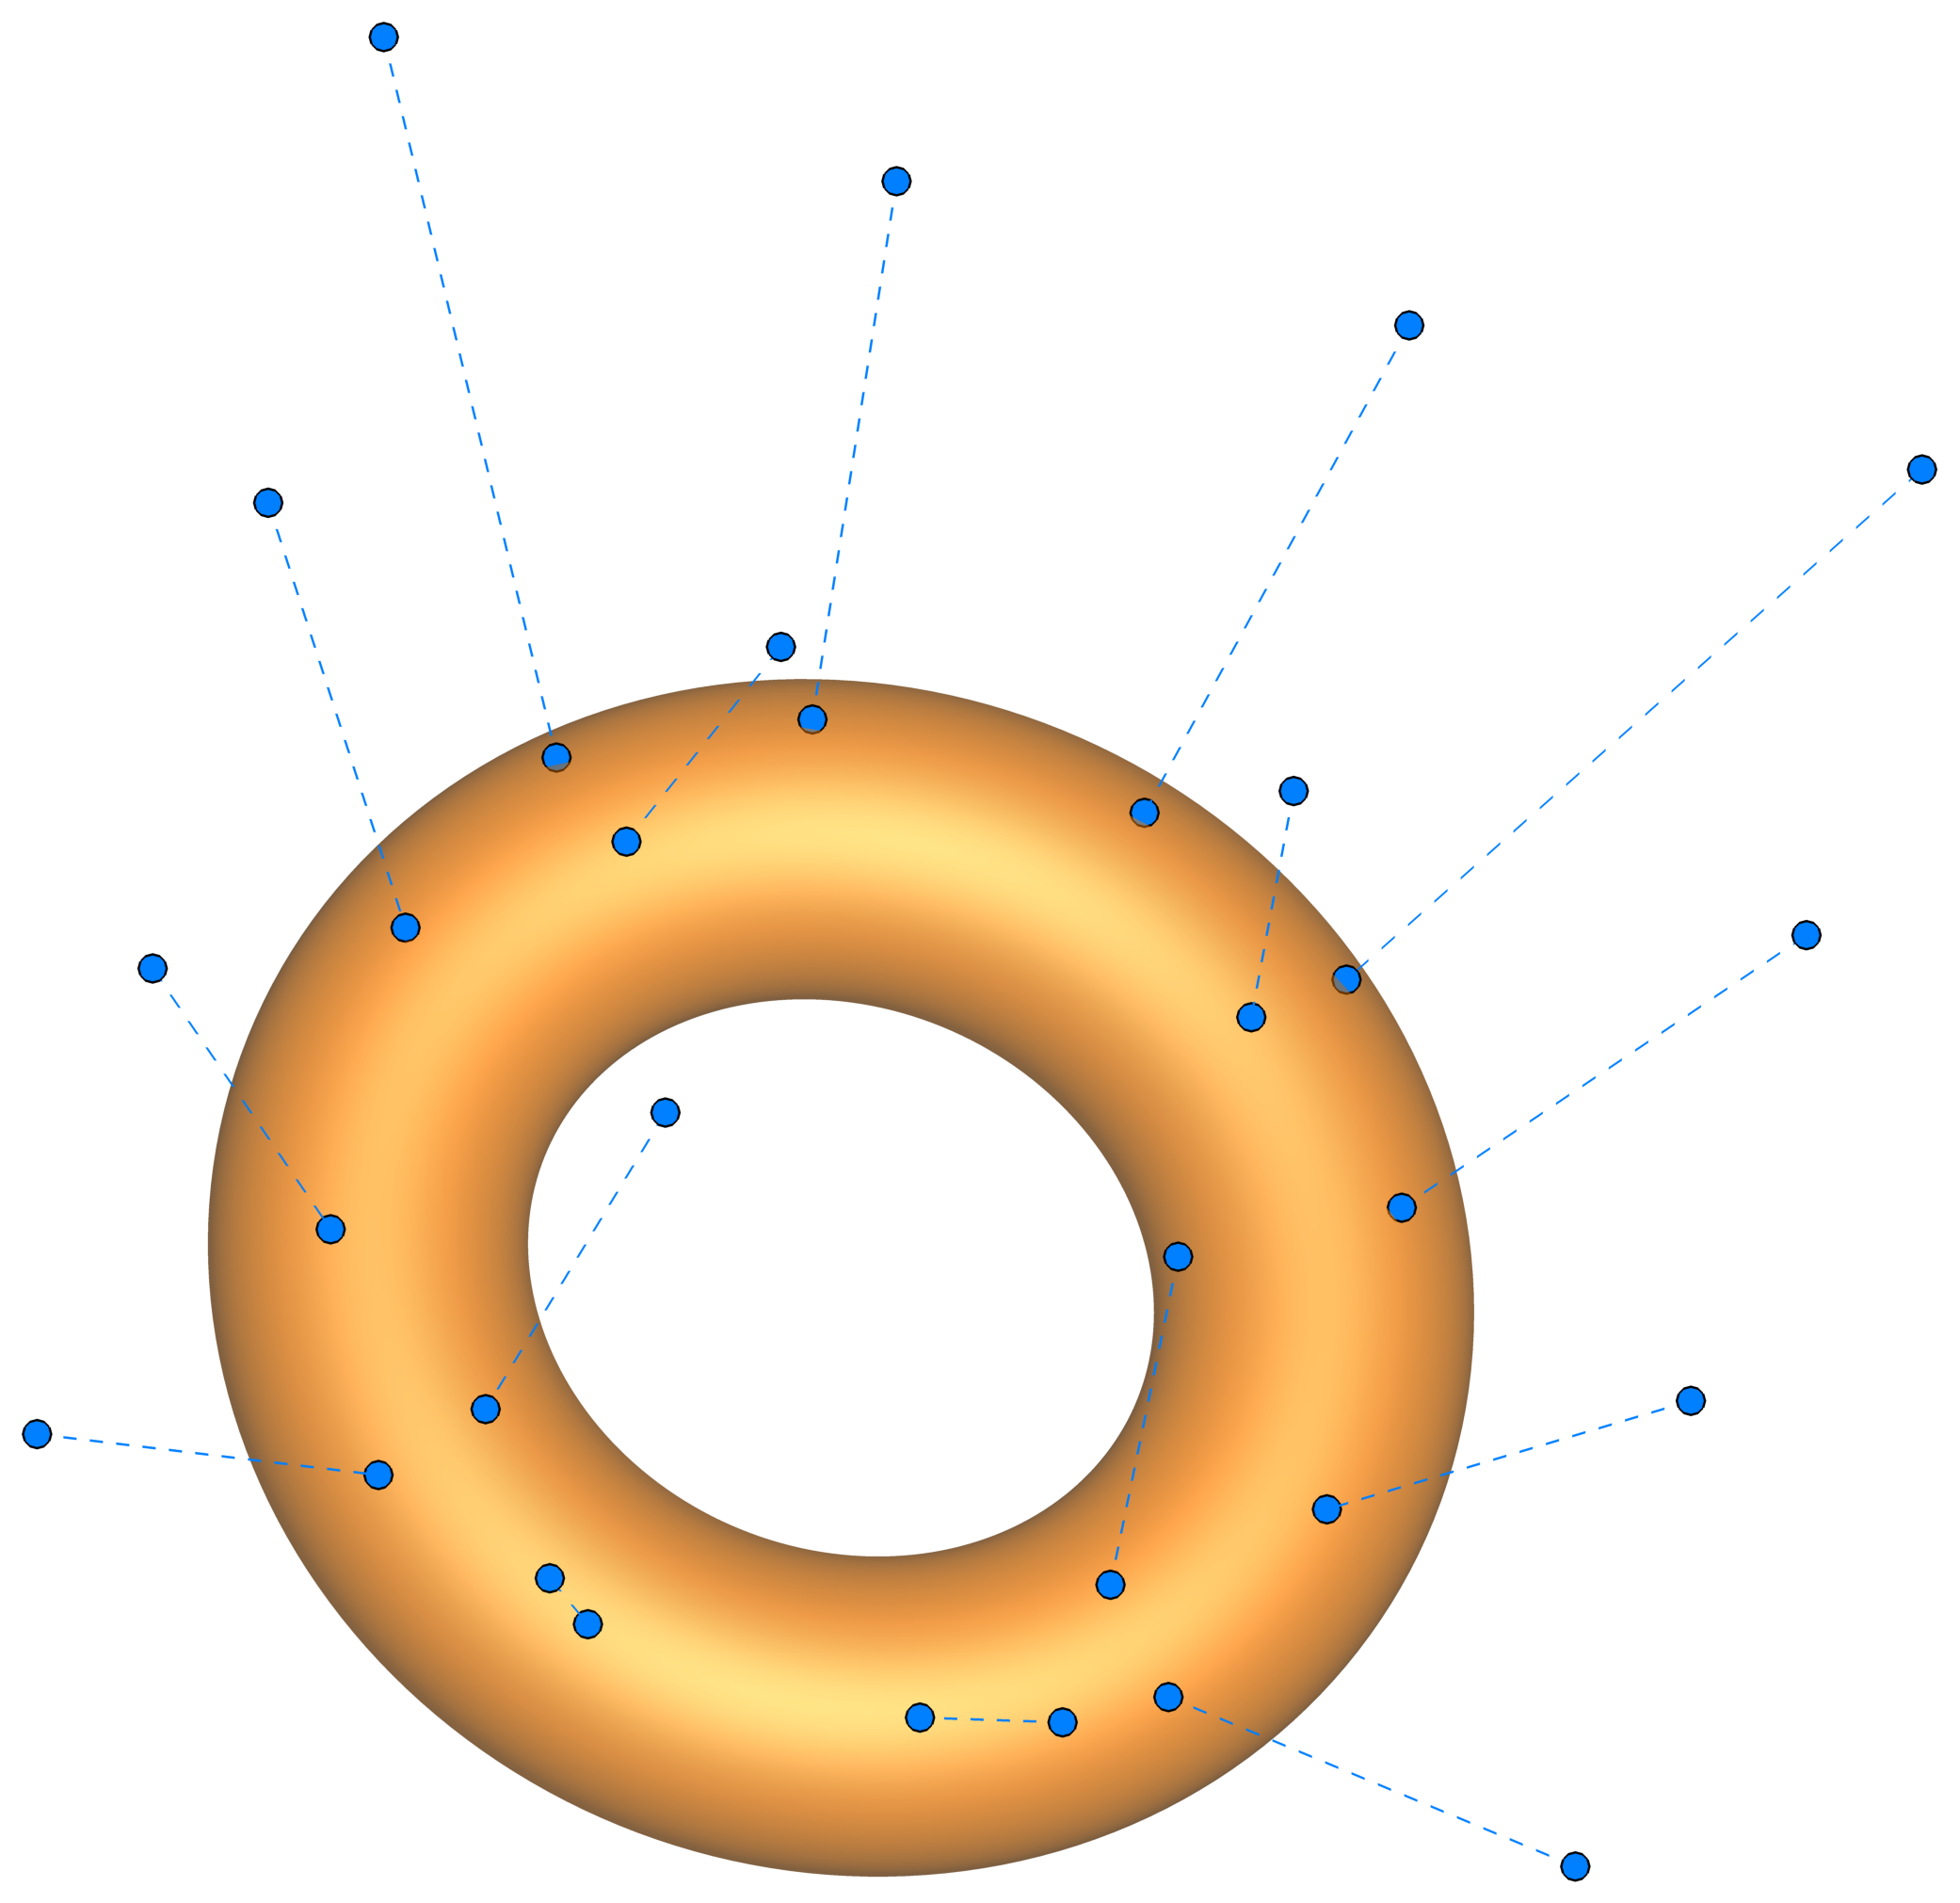
\includegraphics[width=\textwidth]{../tec/projection/02.png}
		\end{subfigure}
		\hspace{0.5cm}
		\begin{subfigure}{.45\textwidth}
			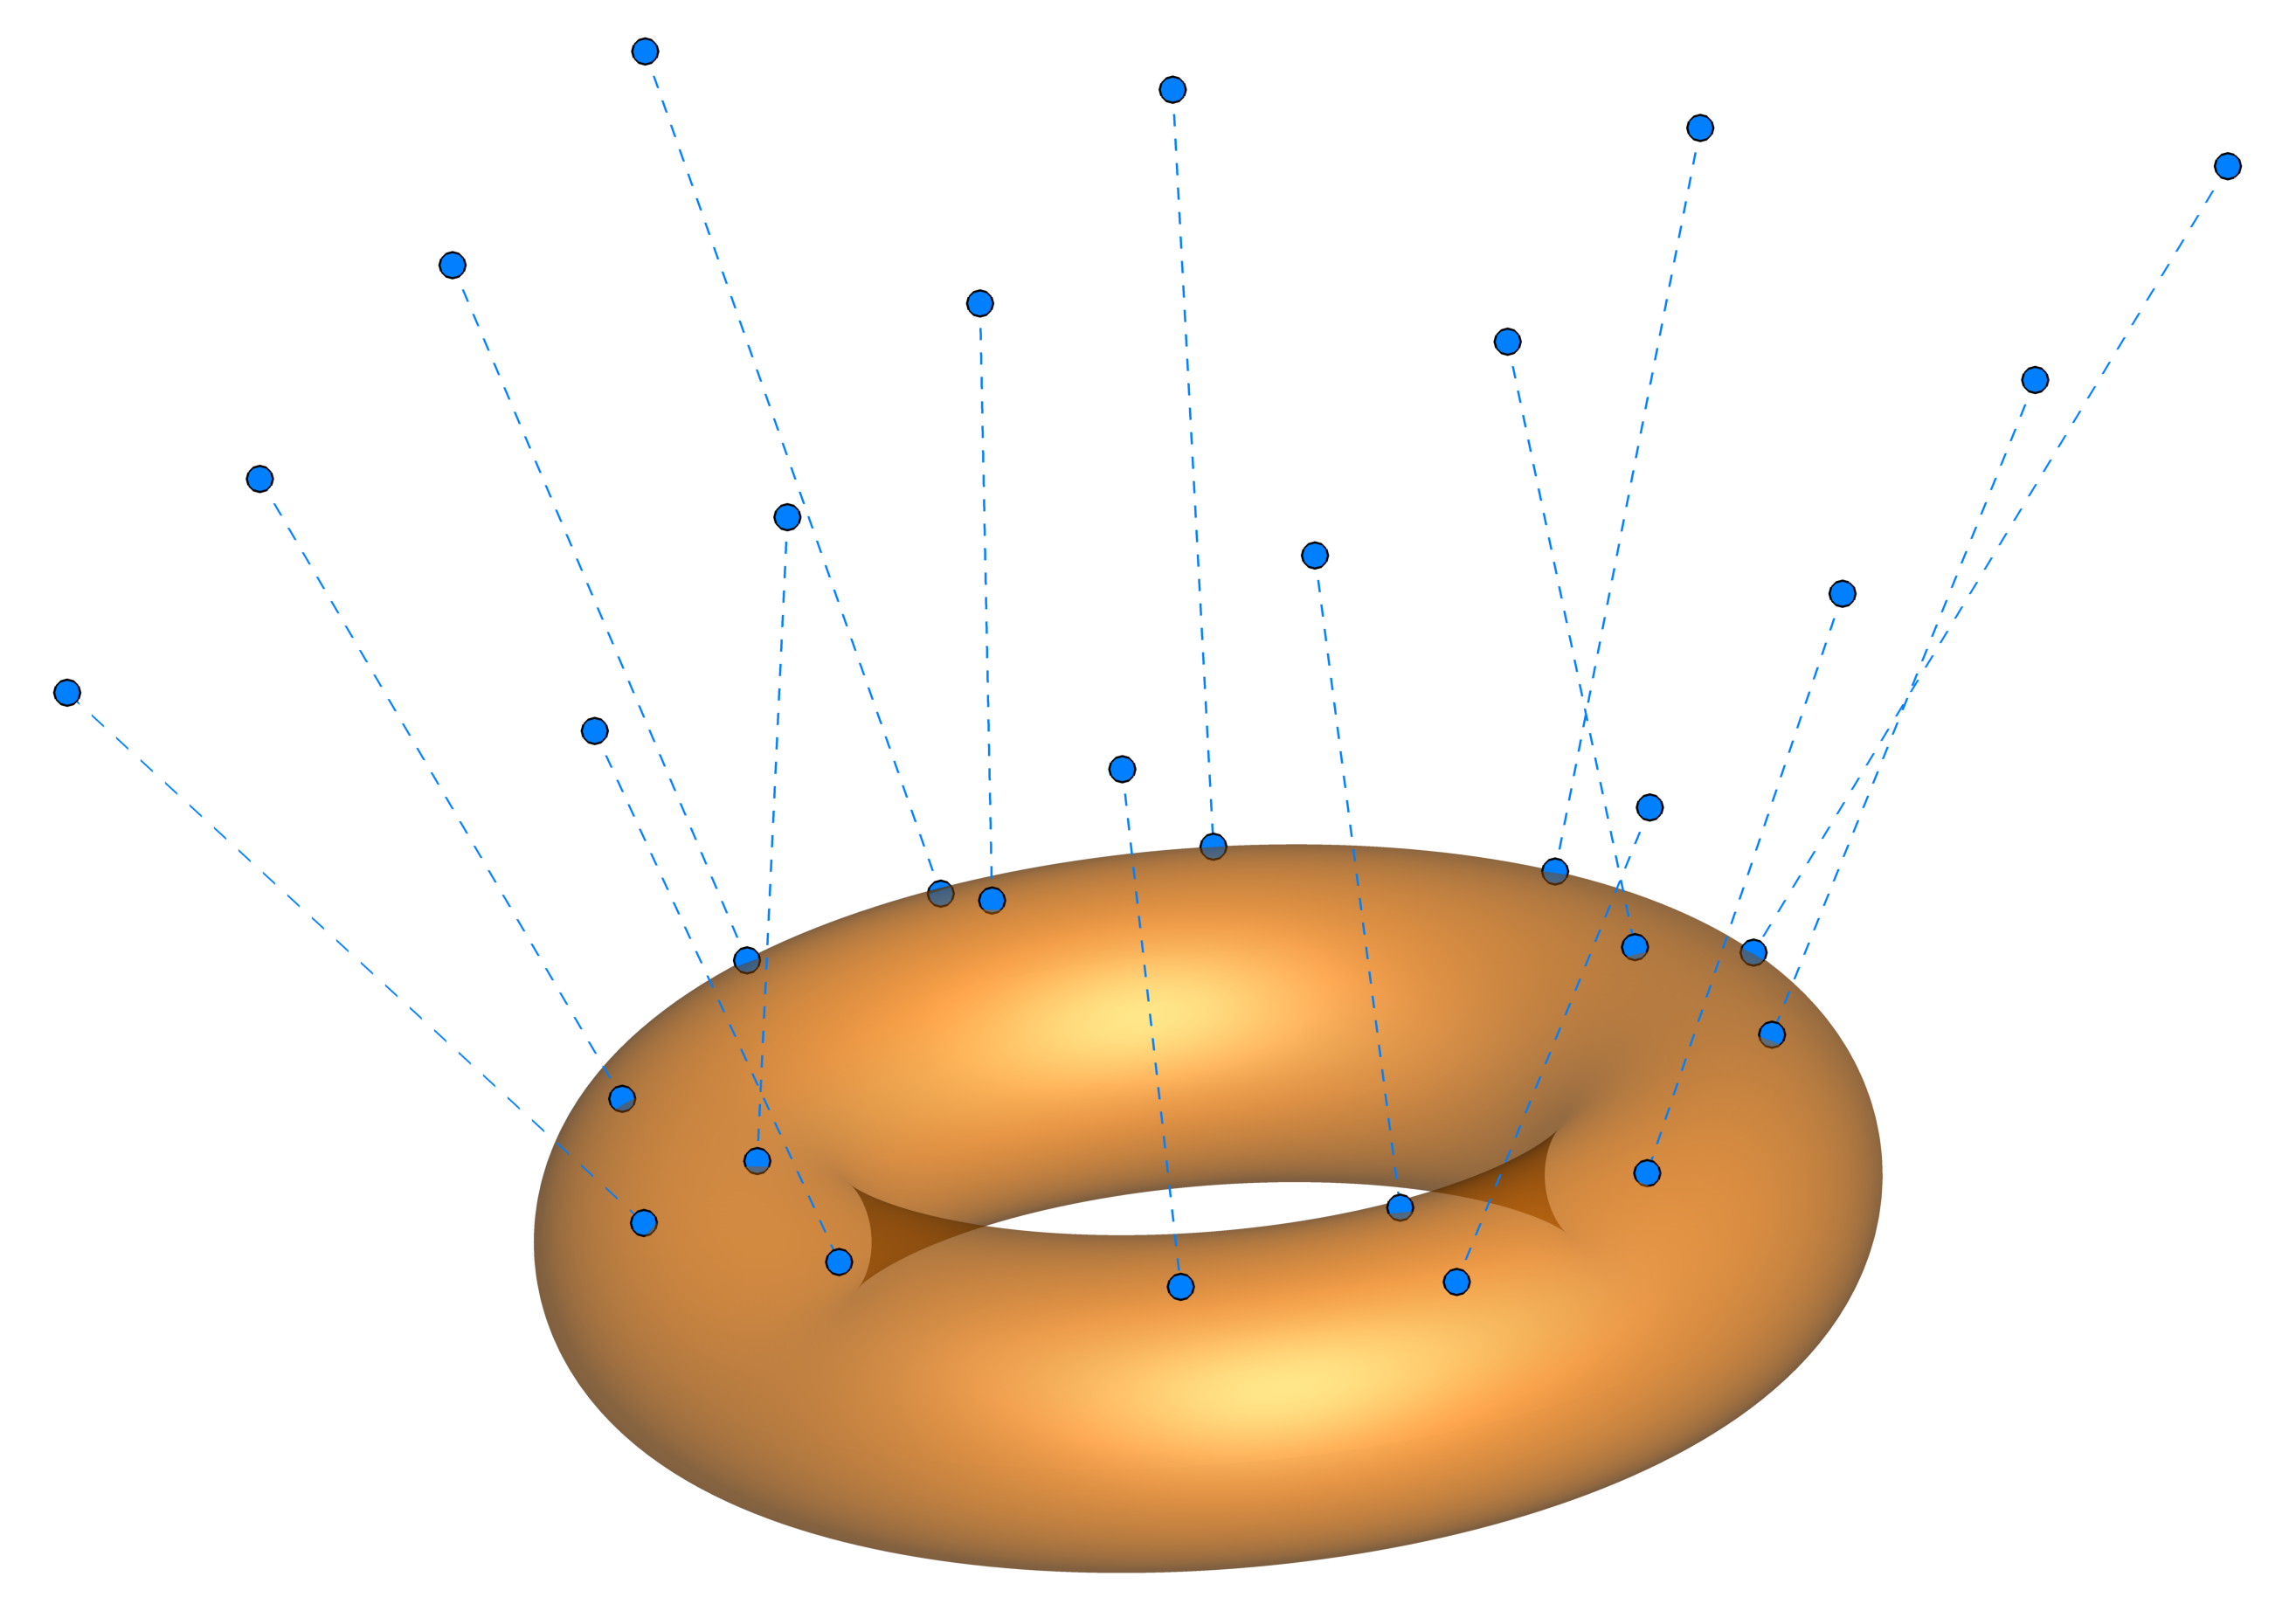
\includegraphics[width=\textwidth]{../tec/projection/01.png}
			\vspace{0.5cm}
		\end{subfigure}
		\caption{Point projection. Each blue point on the orange surface is the projection of the point connected to it with a dotted line.}
	\end{figure}


\subsection{Ray-Curve \& Ray-Surface Intersection}\label{subsec:raymarching}
	This section describes the intersection of a ray and a curve according to \cite{Hart1996}.

	\begin{definition}
		A \emph{ray} with support vector $A \in \mathbb{R}^d$ and direction vector $B \in \mathbb{R}^d$ is given by the set of points
			\begin{equation*}
				\hat R_{A,B} = \{A + tB \;:\; t \in \mathbb{R},\; t \geq 0\}.
			\end{equation*}
		The dependence of a point on the ray on the real parameter $t$ motivates the description of this set as a map
			$$R_{A,B}: \mathbb{R} \rightarrow \mathbb{R}^d,\;\; t \mapsto A+tB.$$
		which yields the equation $\hat R_{A,B} = R_{A,B}([0,\infty))$.
	\end{definition}

	More formally, we want to find an algorithm that intersects a curve $\gamma(t)$ with $t \in [0, 1]$ with a ray $R_{A,B}(s)$ with $s \in [0, \infty)$. Generally, the intersection of these two sets can be written as
		$$I = \gamma([0,1]) \cap R_{A,B}([0,\infty)).$$
	The algorithm presented will return only up to one element in that set, specifically the one corresponding to the lowest value of the ray parameter $s$. If however $I = \emptyset$, then no element will be returned.

	\begin{definition}
		Let $R_{A,B}$ a ray and $\gamma(t)$ a curve. Then the ray-curve-distance w.r.t $R_{A,B}$ and $\gamma$ is defined as
			$$ D(R_{A,B}, \gamma) := D(\gamma, R_{A,B}) := \underset{s\in[0,\infty)}{\min} \; D(\gamma, R_{A,B}(s))$$
	\end{definition}
	
	\begin{definition}\label{def:raycollisionparameter}
		Let $R_{A,B}(s)$ a ray and $\gamma(t)$ a curve. If a solution to 
			$$\underset{s\in[0,\infty)}{\min} \; s \quad \text{subject to} \quad D(\gamma, R_{A,B}(s)) = 0$$
		exists, then it is called \emph{collision parameter} of $R_{A,B}$ w.r.t. $\gamma$.
	\end{definition}

	We define the return value of our algorithm as the one element set given by
		$$ I_{\min} := 
			\begin{cases}
				\{R_{A,B}(s^*)\} 	&\text{if } D(R_{A,B}(s^*), \gamma) \leq \epsilon, \\
				\emptyset			&\text{otherwise,}	
			\end{cases}
		$$
	where the absolute tolerance $\epsilon > 0$ is close to $0$ and $s^*$ is an approximation of the collision parameter of $R_{A,B}$ w.r.t. $\gamma$. If $I_{\min} \neq \emptyset$, then we refer to the element in $I_{\min}$ as \emph{collision point}.

	\begin{remark}
		Why is the notion of the collision point of interest? To exemplify the prospect of our algorithm, imagine the following scenario: Let there be a reflective interface represented by a curve $\gamma$ and a beam of light represented by a ray $R_{A,B}$. Then our model suggests the equivalence of the physical point of reflection and the collision point of the ray with respect to the curve.
	\end{remark}

	We can find the approximation $s^*$ of the collision parameter by using a common CAD scheme called \emph{ray marching}, in which we traverse the ray $R_{A,B}$ by small distance increment s$s$ until we achieve collision with the curve $\gamma$. How do we choose the optimal value for $s$? The idea is the following: Using the point projection algorithm, we can calculate the \emph{safe distance} $s$ of the point $A$ on the ray to the curve $\gamma$. Then we can easily construct a point $P$ that fulfills $D(A,P) = s$ and lies on the ray $R_{A,B}$ by 
		$$ P := A+s\frac{B}{||B||}.$$
	Now there are only two possibilities: Either $P$ lies within the $\epsilon$-ball of the collision point, or the line segment $\overline{AP} \subset R_{A,B}([0,\infty))$ has at least $\epsilon$ distance to $\gamma$. In the first case, we can return $\{P\}$. In the second case, we can repeat the procedure on the set 
		$$ R_{A,B}([0,\infty)) \setminus \overline{AP} = R_{A,B}([s,\infty)) = R_{P,B}([0,\infty)).$$
	If after a certain amount of iterations $N$ the algorithm does not converge to a point which lies within the $\epsilon$-ball of the collision point, we return $\emptyset$.

	\begin{figure}[H]
		\centering
		\includesvg[width=0.8\textwidth]{../python/rayMarching}
		\caption{Ray marching.}
		\label{fig:raymarchingvis}
	\end{figure}

	Figure \ref{fig:raymarchingvis} describes ray marching visually. At each iteration, a new safe distance $s$ (depicted as green circle radii) along the ray is calculated. The ray is traversed using $s$ as step size (to achieve the points depicted in green) until the safe distance falls below the absolute tolerance $\epsilon$. The resulting point, depicted in purple, is close to the collision point. The implementation of ray marching algorithm given a point projection algorithm proves to be relatively simple.

	\begin{algorithm}[H]
		\begin{algorithmic}[1]

			\caption{Ray Marching}\label{alg:raymarching}
			\Procedure{intersectCurveRay}{$\gamma, A, B$}
				\State $B \gets \frac{B}{||B||}, s \gets 0, P \gets A$
				\For {$k = 1, 2,..., N$}
					\State $s \gets D(\gamma(\text{pointProjection}(\gamma, P)), P)$
					\State $P \gets P + sB$
					\If {$s < \epsilon$}
						\State \Return $\{P\}$
					\EndIf
				\EndFor

				\State \Return $\emptyset$
			\EndProcedure
		\end{algorithmic}
	\end{algorithm}

	Using the point projection algorithm for surfaces (instead of the point projection algorithm for curves) to find the distance between a point and a surface, we can easily generalize this algorithm to find the intersection of a ray and a surface. Formally, the only difference between the curve and the surface version of the algorithm lie in the point projection, which was described in Section \ref{subsec:pointproj}.

\subsection{Intersecting Two Curves in 2D}
	In order to trim curves at intersection points, we require the pair of parameters at which two curves intersect. Let $\gamma_1(s)$ and $\gamma_2(t)$ be two continuous curves in $\mathbb{R}^2$ with $s,t \in [0,1]$ which intersect at finitely many points at most. In this section, we seek for the set of parameters at which these curves intersect.

	\begin{definition}
		The distance between two curves $\gamma_1, \gamma_2$ is defined as
			$$ D(\gamma_1, \gamma_2) := \min_{(s,t) \in [0,1]^2} D(\gamma_1(s), \gamma_2(t)).$$
	\end{definition}

	Similarly to the prior sections, our goal is to minimize a distance function $D(\gamma_1(s), \gamma_2(t))$. In this case, we will employ a pragmatic scheme that uses a piecewise linear approximation of the curve, in which finding intersections is comparably simple and involves finding the intersection of a number of line segments.

	\begin{definition}
		The intersection parameter set of two continuous curves $\gamma_1$ and $\gamma_2$ is defined as
				$$ I(\gamma_1, \gamma_2) := \{(s,t) \in [0,1]^2 : \gamma_1(s) = \gamma_2(t)\}.$$
		Notice that $\gamma_1([0,1]) \cap \gamma_2([0,1]) = \emptyset$ if and only if $I(\gamma_1, \gamma_2) = \emptyset$.
	\end{definition}

	\begin{figure}[H]
		\centering
		\includesvg[width=\textwidth]{../python/curveIntersectionConnectedness}
		\caption{In (A) we have $|I(\gamma_1, \gamma_2)| < \infty$, whereas in (B) we have $|I(\gamma_1, \gamma_2)| = \infty$.}
		\label{fig:curveIntersectionConnectedness}
	\end{figure}

	For the use with CoolingGen, our goal is to find the set $I(\gamma_1, \gamma_2)$ in case of $|I(\gamma_1, \gamma_2)| < \infty$ (see Figure \ref{fig:curveIntersectionConnectedness}).

	\begin{definition}\label{def:linesegdef}
		The line segment between the points $A_s = (A_{s_x}, A_{s_y})^T$ and $A_e = (A_{e_x}, A_{e_y})^T$ is defined as the set
			$$ \overline{A_s A_e} := \{(1-t)A_s + tA_e : t \in [0,1]\}. $$
		The dependence of a point on the line segment on the real parameter $t$ motivates the description of this set as a map
			$$ L_A : \mathbb{R} \rightarrow \mathbb{R}^d, \quad t \mapsto (1-t)A_s + tA_e,$$
		which yields the equation $\overline{A_s A_e} = L_A([0,1])$. Notice that given the definition of the direction vector $A_d := A_e - A_s = (A_{d_x}, A_{d_y})$, we can write
			$$ L_A(t) = A_s + tA_d.$$
	\end{definition}
	
	We write the derivative of a curve $\gamma(t)$ as $\nabla \gamma(t) := \gamma'(t)$. The key idea of our algorithm is described by the following theorem.

	\begin{theorem}\label{thm:parallelintersection}
		Let $\gamma_1$ and $\gamma_2$ be two differentiable curves and let $(s^*, t^*) \in I(\gamma_1, \gamma_2) \cap (0,1)^2$. If the curve derivatives $\nabla\gamma_1(s^*)$ and $\nabla\gamma_2(t^*)$ are not parallel, then there exist neighborhoods 
			$$[s^*-\epsilon, s^*+\epsilon] \quad\text{and}\quad [t^*-\epsilon, t^*+\epsilon]$$
		around $s^*$ and $t^*$, respectively, where $\epsilon > 0$ such that the line segments
			$$\overline{\gamma_1(s^*-\epsilon) \, \gamma_1(s^*+\epsilon)} \quad\text{and}\quad \overline{\gamma_2(t^*-\epsilon) \, \gamma_2(t^*+\epsilon)}$$
		intersect. 
	\end{theorem}
	\begin{remark}
 		Suppose that the line segments $\overline{\gamma_1(s_1) \, \gamma_1(s_2)}$ and $\overline{\gamma_2(t_1) \, \gamma_2(t_2)}$ intersect. We cannot conclude that there is an intersection $(s,t) \in I(\gamma_1, \gamma_2)$ with $s \in [s_1, s_2]$ and $t \in [t_1, t_2]$. Using this theorem as core concept for our algorithm, we will need to ensure that the distance between the target curve segments is zero. In this numerical setting, it is sufficient to instead ensure
 			$$ D(\gamma_1 \domrestr_{[s_1, s_2]}, \gamma_2 \domrestr_{[t_1, t_2]}) \leq \alpha$$
 		for a sufficiently small absolute tolerance $\alpha > 0$. If this is not the case, then no intersection lies inside of $[s_1, s_2] \times [t_1, t_2]$ and every line segment intersection found within should be discarded. Here, the notation $\gamma \domrestr{M}$ for some parametric curve $\gamma$ and a subset $M \in [0,1]$ is the domain restriction of $\gamma$ onto $[a,b]$.
	\end{remark}
	
	\begin{figure}[H]
		\centering
		\includesvg[width=0.4\textwidth]{../python/linearApproxCircleIntersection}
		\caption{Two curves that intersect in a point tangentially and their linear approximations.}
		\label{fig:tangentialintersection}
	\end{figure}

	What Theorem \ref{thm:parallelintersection} and it's Remark tell us is that parallel intersection points (for example in two circular curves that intersect in exactly one point, see Figure \ref{fig:tangentialintersection}) are rarely detected by intersecting a piecewise linear approximation of the curve. In other words, if for any intersection parameter pair $(s^*, t^*) \in I(\gamma_1, \gamma_2)$ we have $\nabla \gamma_1(s^*) = \nabla \gamma_2(t^*)$, then it is likely that the intersection is not detected by the described line segment intersection scheme.
 	
	\begin{theorem}\label{thm:lineintersection}
		Let $L_A([0,1])$ and $L_B([0,1])$ be two line segments in $\mathbb{R}^2$. If the lines $L_A((-\infty,\infty))$ and $L_B((-\infty,\infty))$ are not parallel, their single intersection point is given by $L_A(t_A) = L_B(t_B)$, where
			\begin{equation*}\label{eq:lineintersection}
				t_A = 
				\frac {
					\det
					\begin{pmatrix}
						\Delta S_y 	& \Delta S_x		\\
						B_{d_y}	& B_{d_x}
					\end{pmatrix}
				}
				{
					\det
					\begin{pmatrix}
						B_{d_x} & B_{d_y} 	\\
						A_{d_x} & A_{d_y}
					\end{pmatrix}
				}
				\quad\text{and}\quad
				t_B =
				\frac {
					\det
					\begin{pmatrix}
						\Delta S_y 	& \Delta S_x		\\
						A_{d_y}	& A_{d_x}
					\end{pmatrix}
				}
				{
					\det
					\begin{pmatrix}
						B_{d_x} & B_{d_y} 	\\
						A_{d_x} & A_{d_y}
					\end{pmatrix}
				},
			\end{equation*}
		where $\Delta S = B_s - A_s$ and $t_A, t_B \in \mathbb{R}$. If $t_A \in [0,1] \wedge t_B \in [0,1]$, the line segments intersect in a single point.
	\end{theorem}
	
	In our algorithm we sample the curves $\gamma_1$ and $\gamma_2$ at $t_i = \frac{i}{N}$, where $i \in \{0,...,N\}$. In the next step we check for an intersection of 
		$$\overline{\gamma_1(t_i) \, \gamma(t_{i+1})} \quad\text{and}\quad \overline{\gamma_2(t_j) \, \gamma_2(t_{j+1})}$$
	for $i,j \in \{0,...,N-1\}$. For all intersection pairs $(i^*, j^*)$, we calculate the interval midpoint distance
		$$D \left( \gamma_1 \left( \frac{t_{i^*} + t_{i^*+1}}{2} \right), \gamma_2 \left( \frac{t_{j^*} + t_{j^*+1}}{2} \right) \right)$$
	and recursively repeat this procedure on the curves $\gamma_1([t_i, t_{i+1}])$ and $\gamma_2([t_j, t_{j+1}])$. If after a given recursion depth, the interval midpoint distance of some pair $(i^*, j^*)$ is greater than a given absolute tolerance $\alpha$, we discard $(i^*, j^*)$.
	
	The sampling into a piecewise linear interpolation of any curve will be handled by the following algorithm.
	\begin{algorithm}[H]
		\begin{algorithmic}[1]
			\Input
				\Desc{$\gamma$}{curve on $[0,1]$}
				\Desc{$l,u$}{lower and upper bound inside of $[0,1]$}
				\Desc{$N$}{number of line segments that approximate the curve}
			\EndInput

			\caption{Calculating the piecewise linear interpolation}\label{alg:samplecurve}
			\Procedure{piecewiseLinInterp}{$\gamma, l, u, N$}
				\State $P \gets \text{empty vector with } N+1 \text{ entries}$
				\For {$i = 0, ..., N$}
					\State $P_i \gets \gamma \left( (u-l) \frac{i}{N} + l \right)$
				\EndFor
				\State \Return $P$
			\EndProcedure
		\end{algorithmic}
	\end{algorithm}
	
	Calculating whether two line segments intersect is a constant time operation. For each recursion depth, this operation is executed $N^2$ times, granting the total performance of $O(N^2)$.

	\begin{figure}[H]
		\centering
		\includesvg[width=0.9\textwidth]{../python/piecewiseLinearIntersection}
		\caption{Demonstration of the curve intersection algorithm. Figure (A) shows the input curves, Figure (B) the different steps and Figure (C) the result. The dots on the curve represent the samples on the curve. The red lines represent the intersection of two line segments.}
		\label{fig:piecewiselinearintersection}
	\end{figure}
	
	The algorithm in Figure \ref{fig:piecewiselinearintersection} first calculates estimates of the intersection points and then refines those estimates until the target distance falls below $\alpha$. If a maximum recursion depth $d_{\max}$ is reached before falling below target distance, the estimated point is not returned. Using Algorithm \ref{alg:samplecurve} and writing the procedure from Theorem \ref{thm:lineintersection} as function \texttt{lineSegmentsIntersect}, which returns \texttt{true} if and only if the input line segments intersect, we can write the curve intersection algorithm as follows.

	\begin{algorithm}[H]
		\begin{algorithmic}[1]
			\Input
				\Desc{$\gamma_1, \gamma_2$}{curves on $[0,1]$}
				\Desc{$d_{\max}$}{maximum recursion depth}
				\Desc{$\alpha$}{absolute tolerance value}
			\EndInput
			\Output
				\Desc{$I(\gamma_1, \gamma_2)$}{intersection parameter set}
			\EndOutput

			\caption{Curve Intersection}\label{alg:curveintersection}
			\Procedure{intersectCurvesRecursion}{$I, \gamma_1, l_1, u_1, \gamma_2, l_2, u_2, d$}
				\State $m_1 \gets \frac{l_1 + u_1}{2}$ and $m_2 \gets \frac{l_2 + u_2}{2}$
				
				\If {$D(\gamma_1(m_1), \gamma_2(m_2)) \leq \alpha$} append $(m_1, m_2)$ to $I$ and \Return
				\EndIf

				\If {$d \geq d_{\max}$} do nothing and \Return
				\EndIf

				\State $P^{(1)} \gets \text{piecewiseLinInterp}(\gamma_1, l_1, u_1, N)$ and $P^{(2)} \gets \text{piecewiseLinInterp}(\gamma_2, l_2, u_2, N)$
				

				\For {$i = 0,...,N-1$}
					\For {$j = 0,...,N-1$}
						\If {$\text{lineSegmentsIntersect}(P^{(1)}_i, P^{(1)}_{i+1}, P^{(2)}_j, P^{(2)}_{j+1})$}
							\State $s_1 \gets (l_1 - u_1) \frac{i}{N} + l_1$ and $s_2 \gets (l_1 - u_1) \frac{i+1}{N} + l_1$
							\State $t_1 \gets (l_2 - u_2) \frac{j}{N} + l_2$ and $t_2 \gets (l_2 - u_2) \frac{j+1}{N} + l_2$
							\State $\text{intersectCurvesRecursion}(I, \gamma_1, s_1, s_2, \gamma_2, t_1, t_2, d+1)$
						\EndIf
					\EndFor
				\EndFor

				\State \Return $I$
			\EndProcedure

			\Procedure{intersectCurves}{$\gamma_1, \gamma_2$}
				\State $I \gets \emptyset$
				\State $\text{intersectCurvesRecursion}(I, \gamma_1, 0, 1, \gamma_2, 0, 1, 0)$

				\State \Return $I$
			\EndProcedure
		\end{algorithmic}
	\end{algorithm}

	Using slight modifications, one can also make use of this algorithm in self-intersection detection of parametric curves. To do this, instead of iterating over all line segments in the first recursion step, we iterate in a triangular manner (in Algorithm \ref{alg:curveintersection}, replace \texttt{[for $j = 0, ..., N-1$]} with \texttt{[for $j = i+2, ..., N-1$]}, but only when calling \texttt{intersectCurvesRecursion} for the first time). Details about self-intersections are presented in the next section.

	As discussed before, this intersection algorithm might not identify an intersection parameter pair $(s,t)$ where $\nabla \gamma_1(s) = \nabla \gamma_2(t)$. It does however prove fast and robust in the case of CoolingGen, where such intersections are currently not of interest.

\subsection{Offset Curves \& Self-Intersections in 2D}\label{sec:offsetcurves}
	Offset curves are an important CAD tool and can be used to model contours of a certain thickness, which is why they are often referred to as parallel curves. Offset curves are paramount in the creation of fillets, which we will elaborate later. Among the variety of methods in CoolingGen, the creation of offset curves proves to be the most useful one, which perhaps lies in the very nature of cooling geometries, most of which are comprised of offset surfaces inside a given turbine blade surface. The definition of offset curves in this thesis is adapted from \cite{Elber1997}.

	\begin{definition}\label{def:offseteasy}
		Let $\gamma(t) = (x(t), y(t)) \in \mathbb{R}^2$ for $t\in[0,1]$ be a differentiable curve. Then $O^\gamma_d(t)$ is called the $d$-offset curve and is defined as
			$$ O^\gamma_d(t) := \gamma(t) + dN^\gamma(t),$$
		where $N^\gamma(t)$ is called the normal of $\gamma(t)$ and defined as
			$$N^\gamma(t) := \frac{\nabla\gamma(t)^\perp}{||\nabla\gamma(t)||}$$
		and
			$$\nabla\gamma(t)^\perp = \left(\derivative{x}{t}(t), \derivative{y}{t}(t)\right)^\perp := \left(-\derivative{y}{t}(t), \derivative{x}{t}(t)\right)$$
		is orthogonal to the gradient of $\gamma(t)$.
	\end{definition}

	\begin{remark}
		Notice that this definition makes the convention of an oriented normal vector, because it will be useful later. The unit vector $-N^\gamma(t)$ is also orthogonal to $\nabla \gamma(t)$.
	\end{remark}

	\begin{figure}[H]
		\centering
		\includesvg[width=0.65\textwidth]{../python/offsetCurveExample}
		\caption{Offset curves of a given curve $\gamma$ for different values of $d$.}
		\label{fig:offsetcurveexample}
	\end{figure}

	As can be observed in Figure \ref{fig:offsetcurveexample}, some $O^\gamma_d$ tend to self-intersect even though $\gamma$ does not self-intersect. We previously established that the non-existence of any self-intersection of a curve is equivalent to its injectivity. In CoolingGen, we are often interested in modelling parallel contours. However, self-intersections do not represent meaningful objects in this context. Specifying the offset value $d$, a user of CoolingGen would expect to find a curve $\overline{O}^\gamma_d$ that at least satisfies the property
	\begin{equation}\label{eq:offsetproperty}
		\min_s \, D(\gamma(s), \overline{O}^\gamma_d) = d.
	\end{equation}
	Informally, if we imagine a ball of radius $d$ to roll along one side of the curve $\gamma$, then $O^\gamma_d(t)$ is injective as long as the ball only touches one point at a time.
	\begin{remark}
		Formally, we are able to define the \emph{curvature} $\kappa^\gamma(t)$ of a curve at any given point, which is equal to the reciprocal of the radius of the tangential sphere of the curve at that point. This notion allows us to make the following observation: If there exists some $t$ such that $\kappa^\gamma(t) > \frac{1}{d}$, then $O^\gamma_d(t)$ is not injective.
	\end{remark}

	If we force injectivity of $O^\gamma_d$ in a certain way, we will be able to guarantee the property in Equation (\ref{eq:offsetproperty}). To do this, we need to find the self-intersections of $O^\gamma_d$.

	\begin{definition}
		The parameter set of self-intersections of a curve $\gamma(t)$ is defined as
			$$ I(\gamma) := \{(s,t) \in [0,1]^2 : \gamma(s) = \gamma(t) \;\wedge\; s < t \}. $$
	\end{definition}

	To find these self-intersections, we can use a slightly modified version of Algorithm \ref{alg:curveintersection}. In the first recursion step of \texttt{intersectCurvesRecursion}, instead of iterating $j$ from $0$ to $N-1$, we are only interested in $j$ from $i+2$ to $N-1$, since for all $(s,t) \in I(O^\gamma_d)$, we have $s < t$. Because $s < t$ each such parameter pair naturally represents an interval subset $[s, t]$ of the parameter space $[0, 1]$.

	\begin{definition}
		For a self-intersection set $I(\gamma)$, we call the set
			$$T(\gamma) := \bigcup_{(s,t) \in I(\gamma)} [s,t]$$
		the trim range of $\gamma$.
	\end{definition}

	We can now choose to only further use and display the curve on $\overline{[0,1] \setminus T(O^\gamma_d)}$ or on $T(O^\gamma_d)$.

	\begin{figure}[H]
		\centering
		\begin{subfigure}{0.49\textwidth}
			\includesvg[width=0.98\textwidth]{../python/offsetCurveSelfIntersection0}
			\caption{Non-injective offset curves.}
		\end{subfigure}
		\begin{subfigure}{0.49\textwidth}
			\includesvg[width=0.98\textwidth]{../python/offsetCurveSelfIntersection1}
			\caption{Trimmed offset curves on $\overline{[0,1] \setminus T(O^\gamma_d)}$.}
		\end{subfigure}
		\caption{Trimming offset curves at their self intersections.}
	\end{figure}

	Now, the restriction $O^{\gamma}_d \domrestr_{T(O^\gamma_d)}$ of the curve $O^{\gamma}_d$ to the trim range $T(O^\gamma_d)$ is not necessarily defined for all $t \in [0,1]$. Similarly, the restriction $O^{\gamma}_d \domrestr_{\overline{[0,1] \setminus T(O^\gamma_d)}}$ of the curve $O^{\gamma}_d$ to the trim range complement $\overline{[0,1] \setminus T(O^\gamma_d)}$ is not necessarily defined for all $t \in [0,1]$. However, we can define a domain scaling map $\xi^M$, that maps a union $M \subset [0,1]$ of finite intervals onto $[0,1]$, where $M$ will be equal to the trim range or its complement. In other words, we want to define a map that allows us to write
		$$O^{\gamma}_d(\xi^M([0,1])) = O^{\gamma}_d (M)$$
	for any finite union $M$ of closed intervals.
	We write the connected components of $M$ as $[s_i, t_i]$ for $i \in \{1,...,m\}$. By setting
		$$ \tilde s_1 := 0 \quad\text{and}\quad \tilde t_m := 1 \quad\text{and}\quad \tilde s_{j+1} := \tilde t_j := \frac{s_{j+1} + t_j}{2} $$
	for $j \in \{1,...,m-1\}$, we can define the maps
		$$ \xi^M_i(t) = 
				\begin{cases}
					\frac{t_i - s_i}{\tilde t_i - \tilde s_i} \; t 	&\text{if } t \in [\tilde s_i, \tilde t_i], \\
					0 												&\text{else},
				\end{cases}
		$$
	that map $[\tilde s_i, \tilde t_i]$ onto $[s_i, t_i]$ and any other value onto $0$. Notice that
		$$ \bigcup_{i=1}^m \; [\tilde s_i, \tilde t_i] = [0,1].$$
	This way, the domain scaling map
		$$ \xi^M(t) = \sum_{i=1}^m \xi^M_i(t) $$
	maps $[0,1]$ onto $M$. Since both $\overline{[0,1] \setminus T(O^\gamma_d)}$ and $T(O^\gamma_d)$ are unions of closed intervals, we can use this procedure to define the trimmed offset curve as
		$$ \overline{O}^\gamma_d (t) = O^\gamma_d \circ \xi^{\overline{[0,1] \setminus T(O^\gamma_d)}}(t)$$
	or 
		$$ \overline{O}^\gamma_d (t) = O^\gamma_d \circ \xi^{T(O^\gamma_d)}(t)$$
	respectively. This curve now satisfies Equation (\ref{eq:offsetproperty}).

	As has been shown, the construction of meaningful offset curves is in no way trivial and requires a multitude of tools. The simple definition of an offset curve (Definition \ref{def:offseteasy}) is only seemingly adequate. Nonetheless, larger offsets, that would lead to self-intersection, are required by the industry. But since self-intersecting curves do no represent sensible objects, we sought for a far more convoluted process.

	In fact, the creation of fillets also plays a role in the creation of offset curves, since the procedure presented leaves behind non-differentiable places on the trimmed offset curves, which are undesirable for CoolingGen's purposes.

\subsection{The Creation of Fillets in 2D}\label{sec:filletcurves}
	Given two curves $\gamma_1$ and $\gamma_2 \in \mathbb{R}^2$ defined on $t \in [0,1]$ we can sometimes construct a circle of a given radius that shares one tangential intersection point with each curve. A circle like this is called a fillet circle. Segments of these circles can replace non-differentiable segments of a curve. We call such segments fillets (see \cite{Sorby2016}). More formally, we can make the following definition.

	\begin{definition}\label{def:filletcircle}
		Let $\gamma_1$ and $\gamma_2$ be two differentiable curves.
		If a curve $\phi^{\gamma_1, \gamma_2}_r$ satisfies the implicit definition
			$$\phi^{\gamma_1, \gamma_2}_r([0,1]) = \{(x,y) : (x-x_0)^2 + (y-y_0)^2 = r^2\}$$
		for a center point $(x_0, y_0)$ and a radius $r$, then it is a circle. If furthermore there exist intersection points
			$$ \gamma_1(s_1) = \phi^{\gamma_1, \gamma_2}_r(\sigma_1) \quad\text{ and }\quad \gamma_2(s_2) = \phi^{\gamma_1, \gamma_2}_r(\sigma_2) $$
		for some $s_1, s_2, \sigma_1, \sigma_2 \in [0,1]$ and these intersection points are tangential in the sense that
			$$
				\frac{\nabla \gamma_1(s_1)}{||\nabla \gamma_1(s_1)||} = 
				\pm\frac{\nabla \phi^{\gamma_1, \gamma_2}_r(\sigma_1)}{||\nabla \phi^{\gamma_1, \gamma_2}_r(\sigma_1)||} 
				\quad\text{ and }\quad 
				\frac{\nabla \gamma_2(s_2)}{||\nabla \gamma_2(s_2)||} =  
				\pm\frac{\nabla \phi^{\gamma_1, \gamma_2}_r(\sigma_2)}{||\nabla \phi^{\gamma_1, \gamma_2}_r(\sigma_2)||},
			$$
		then $\phi^{\gamma_1, \gamma_2}_r$ is a fillet circle of radius $r$ of $\gamma_1$ and $\gamma_2$.
	\end{definition}
	\begin{remark}
		A fillet circle $\phi^{\gamma_1, \gamma_2}_r$ does not necessarily exist for two given curves $\gamma_1$, $\gamma_2$. If a fillet 
		curve $\phi^{\gamma_1, \gamma_2}_{r^*}$ exists for some radius $r^*$, it does usually not exist for all radii $r \in \mathbb{R}$.
	\end{remark}

	\begin{figure}[H]
		\centering
		\includesvg[width=0.6\textwidth]{../python/verySimpleFillet}
		\caption{A fillet curve of radius $1$ and the respective curves $\gamma_1$ and $\gamma_2$.}
		\label{fig:verysimplefillet}
	\end{figure}

	We will find a procedure that yields a fillet circle for a given radius $r$ and a pair of curves $\gamma_1, \gamma_2$ if it exists and returns nothing otherwise. We only need to find the center point $(x_0, y_0)$. Then we can use the parametric definition of a circle and write
		$$ \phi^{\gamma_1, \gamma_2}_r(t) = (r \cos(2 \pi t) + x_0, r \sin(2 \pi t) + y_0).$$
	For example, as shown in Figure \ref{fig:verysimplefillet}, given the curves $\gamma_1(t) = (2t-1,1)$ and $\gamma_2 = (1,2t-1)$ and a radius $r = 1$, the center point $(x_0,y_0)$ of the fillet circle is equal to $(0,0)$. Therefore, in this case,
		$$ \phi^{\gamma_1, \gamma_2}_r(t) = (\cos(2\pi t), \sin(2\pi t)), $$
	which is the unit circle.

	\begin{theorem}\label{thm:fillettheorem}
		Let $\gamma_1, \gamma_2$ and $r$ such that a fillet circle $\phi^{\gamma_1, \gamma_2}_r$ exists. Then the midpoint $M = (x_0, y_0)$ of a fillet circle is given by
			$$ M = O^{\gamma_1}_{\pm r}(s_1) = O^{\gamma_2}_{\pm r}(s_2) $$
		for $(s_1,s_2) \in I(O^{\gamma_1}_{\pm r}, O^{\gamma_2}_{\pm r})$.
	\end{theorem}
	\begin{proof}
		Let $\tilde\phi(t) = r (\sin 2\pi t, \cos 2\pi t) + O^{\gamma_1}_r(s_1)$. Then we can calculate
		\begin{align*}
			\tilde\phi(t) 	&= r (\sin 2\pi t, \cos 2\pi t) + \gamma(s_1) \pm rN^\gamma(s_1) \\
							&= r (\sin 2\pi t, \cos 2\pi t) + \gamma(s_1) \pm r\frac{\nabla\gamma(s_1)^\perp}{||\nabla\gamma(s_1)||}.
		\end{align*}
		Notice that $(\sin 2\pi t, \cos 2\pi t)$ is equal to an arbitrary unit vector, so for some fixed $\sigma_1 \in [0,1]$ the equation
			$$(\sin 2\pi \sigma_1, \cos 2\pi \sigma_1) = \frac{\nabla\gamma(s_1)^\perp}{||\nabla\gamma(s_1)||}$$
		will be satisfied, since $\frac{\nabla\gamma(s_1)^\perp}{||\nabla\gamma(s_1)||}$ is a fixed unit vector.
		In the same manner, we can construct $\sigma_2$ for the equivalent curve definition $\tilde\phi(t) = r (\sin 2\pi t, \cos 2\pi t) + O^{\gamma_2}_r(s_2).$ Notice that $\sigma_1$ and $\sigma_2$ also satisfy
			$$ \tilde\phi(\sigma_1) = \gamma_1(s_1) \quad\text{and}\quad \tilde\phi(\sigma_2) = \gamma_2(s_2).$$
		By calculating $\nabla \tilde\phi(t)$, we find
			$$ \nabla \tilde\phi(t) = 2\pi (\cos 2\pi t, -\sin 2\pi t), $$
		which after normalization yields the equalities
			$$
				\frac{\nabla \gamma_1(s_1)}{||\nabla \gamma_1(s_1)||} = 
				\pm\frac{\nabla \tilde\phi^{\gamma_1, \gamma_2}_r(\sigma_1)}{||\nabla \tilde\phi^{\gamma_1, \gamma_2}_r(\sigma_1)||} 
				\quad\text{ and }\quad 
				\frac{\nabla \gamma_2(s_2)}{||\nabla \gamma_2(s_2)||} =  
				\pm\frac{\nabla \tilde\phi^{\gamma_1, \gamma_2}_r(\sigma_2)}{||\nabla \tilde\phi^{\gamma_1, \gamma_2}_r(\sigma_2)||}.
			$$
		Therefore, $\tilde \phi$ is in fact a fillet circle.
	\end{proof}

	Theorem \ref{thm:fillettheorem} tells us we can use offset curve and intersection methods to find the center point $(x_0, y_0)$ in the general case using the following steps given a radius $r$ and two curves $\gamma_1$ and $\gamma_2$.
	\begin{enumerate}
		\item Calculate the two offset curves $O^{\gamma_1}_r$ and $O^{\gamma_2}_r$.
		\item Find their intersection parameter set $I(O^{\gamma_1}_r, O^{\gamma_2}_r)$.
		\item For $(s,t) \in I(O^{\gamma_1}_r, O^{\gamma_2}_r)$, set $(x_0, y_0) := O^{\gamma_1}_r(s) = O^{\gamma_2}_r(t)$.
	\end{enumerate}

	\begin{figure}[H]
		\centering
		\includesvg[width=\textwidth]{../python/filletConstruction1}
		\caption{Construction of the fillet circle of different radii.}
		\label{fig:filletconstruction}
	\end{figure}

	As can be seen in Figure \ref{fig:filletconstruction}, the curve $\phi^{\gamma_1, \gamma_2}_r$ constructed this way fulfills the requirements of Definition \ref{def:filletcircle} and therefore is a fillet circle. Given the fillet circle, we now only need to trim the curves $\gamma_1$ and $\gamma_2$ and $\phi^{\gamma_1, \gamma_2}_r$.

	\begin{figure}[H]
		\centering
		\includesvg[width=\textwidth]{../python/filletConstruction2}
		\caption{Trimmed curves and fillets}
	\end{figure}

	In CoolingGen, the curves which we want to connect by a fillet are always connected at their boundary points. Without loss of generality, we let $\gamma_1(0) = \gamma_2(0)$. The trimmed input curves are then given by
		$$
			\overline{\gamma_1}(s) = \gamma_1 \domrestr_{[s^*,1]}\left(\frac{s-s^*}{1-s^*}\right) 
			\quad\text{and}\quad
			\overline{\gamma_2}(t) = \gamma_2 \domrestr_{[t^*,1]}\left(\frac{t-t^*}{1-t^*}\right) 
		$$
	for $(s^*,t^*) \in I(O^{\gamma_1}_r, O^{\gamma_2}_r)$. The parameters $s$ and $t$ are scaled such that the domains of the trimmed curves $\overline{\gamma_1}$ and $\overline{\gamma_2}$ remain equal to $[0,1]$.

	Now, instead of actually trimming $\phi^{\gamma_1, \gamma_2}_r$, we can construct a circular arc between the end points $D_i := \overline{\gamma_i}(0)$ of the trimmed curves for $i \in \{1,2\}$. Let $M = (x_0, y_0)$ the fillet circle center. By sweeping the line segment $\overline{M D_1}$ by a certain angle $\Theta$, we can retrieve $\overline{\phi}^{\gamma_1, \gamma_2}_r$. This angle can be calculated by
		$$ \Theta = \arccos \frac{\langle D_1-M, D_2-M \rangle}{||D_1-M|| \; ||D_2-M||}, $$
	where $\langle \cdot, \cdot \rangle$ is the standard scalar product. We can now write the trimmed fillet curve as
		$$ \overline{\phi}^{\gamma_1, \gamma_2}_r(t) = R_{+t\Theta}(D_1-M)+M = R_{-t\Theta}(D_2-M)+M,$$
	for $t \in [0,1]$, where $R_{\Theta}$ is the rotation matrix given by
		\begin{equation}
			R_{t\Theta} :=
			\begin{pmatrix}
				\cos t\Theta & -\sin t\Theta \\
				\sin t\Theta & \phantom{+}\cos t\Theta
			\end{pmatrix}.
			\label{eq:rotationmat}
		\end{equation}
	We are now left with the two trimmed input curves $\overline{\gamma_1}$ and $\overline{\gamma_2}$ and the fillet curve $\overline{\phi}^{\gamma_1, \gamma_2}_r(t)$.

\subsection{Intersecting a Surface \& a Plane}\label{sec:surfaceplaneintersection}
	In this section, we present an algorithm that intersects a plane and a surface in $\mathbb{R}^3$, which is largely motivated by \cite{Barnhill1990}. The intersection generally takes the form of a surface, a curve, a point or any union of the aforementioned. In the case of CoolingGen, we only care about the case that the surface-plane intersection is a single curve. This assumption is implicitly made in many of the statements involving the intersection algorithm. First, we need to introduce some basic notions.

	\begin{definition}
		A plane $P$ with support vector $S \in \mathbb{R}^3$ and normal vector $N \in \mathbb{R}^3$ with $||N|| = 1$ is given by the set
			$$ P_{S,N} := \{S+V : \mathbb{R}^3 \ni V \perp N\}. $$
		It should be noted that for $\tilde S \in P_{\tilde S, N}$ we have the identity $P_{\tilde S, N} = P_{S, N}$. In other words, the choice of the support vector is arbitrary as long as it lies in the same plane.
	\end{definition}

	\begin{figure}[H]
		\centering
		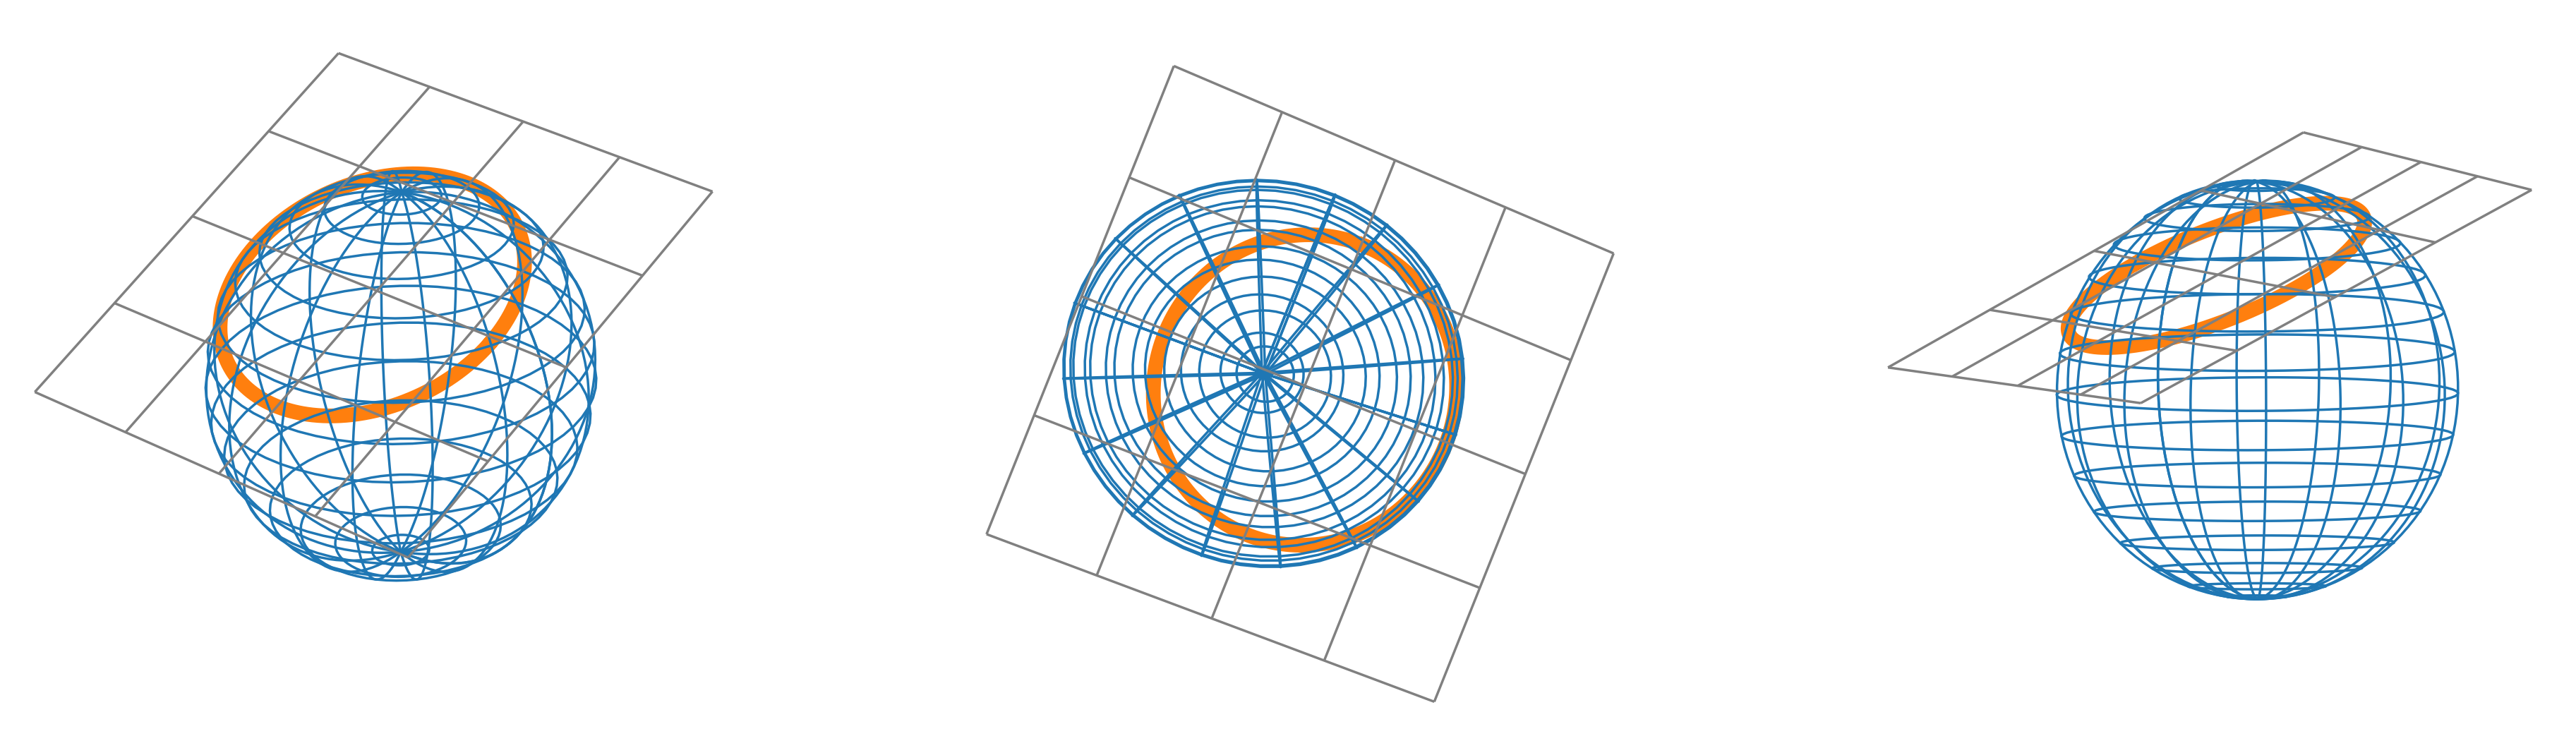
\includegraphics[width=\textwidth]{../python/surfacePlaneIntersection1_cropped.png}
		\caption{The intersection of a surface and a plane generally does not yield a curve. For our purposes, however, this type of intersection is the only case of interest.}
		\label{fig:planeintersectionexample}
	\end{figure}

	\begin{definition}\label{def:distanceplane}
		The distance between a plane $P_{S,N}$ and a point $Q \in \mathbb{R}^3$ is defined as
			$$ D(P_{S,N}, Q) := \underset{V \in P_{S,N}}{\min} \; D(V, Q). $$
	\end{definition}

	\begin{theorem}\label{thm:planeprojection}
		The projection of a point $Q \in \mathbb{R}^3$ onto the plane $P_{S,N}$ is given by
			$$Q_\textrm{proj} := Q - \langle Q - S, N \rangle N,$$
		where $\langle \cdot,\cdot \rangle$ is the standard scalar product. This projection yields the unique solution
			$$ Q_\textrm{proj} = \underset{V \in P_{S,N}}{\arg\min} \; D(V, Q) $$
		to the minimization problem in \ref{def:distanceplane}.
	\end{theorem}

	\begin{figure}[H]
		\centering
		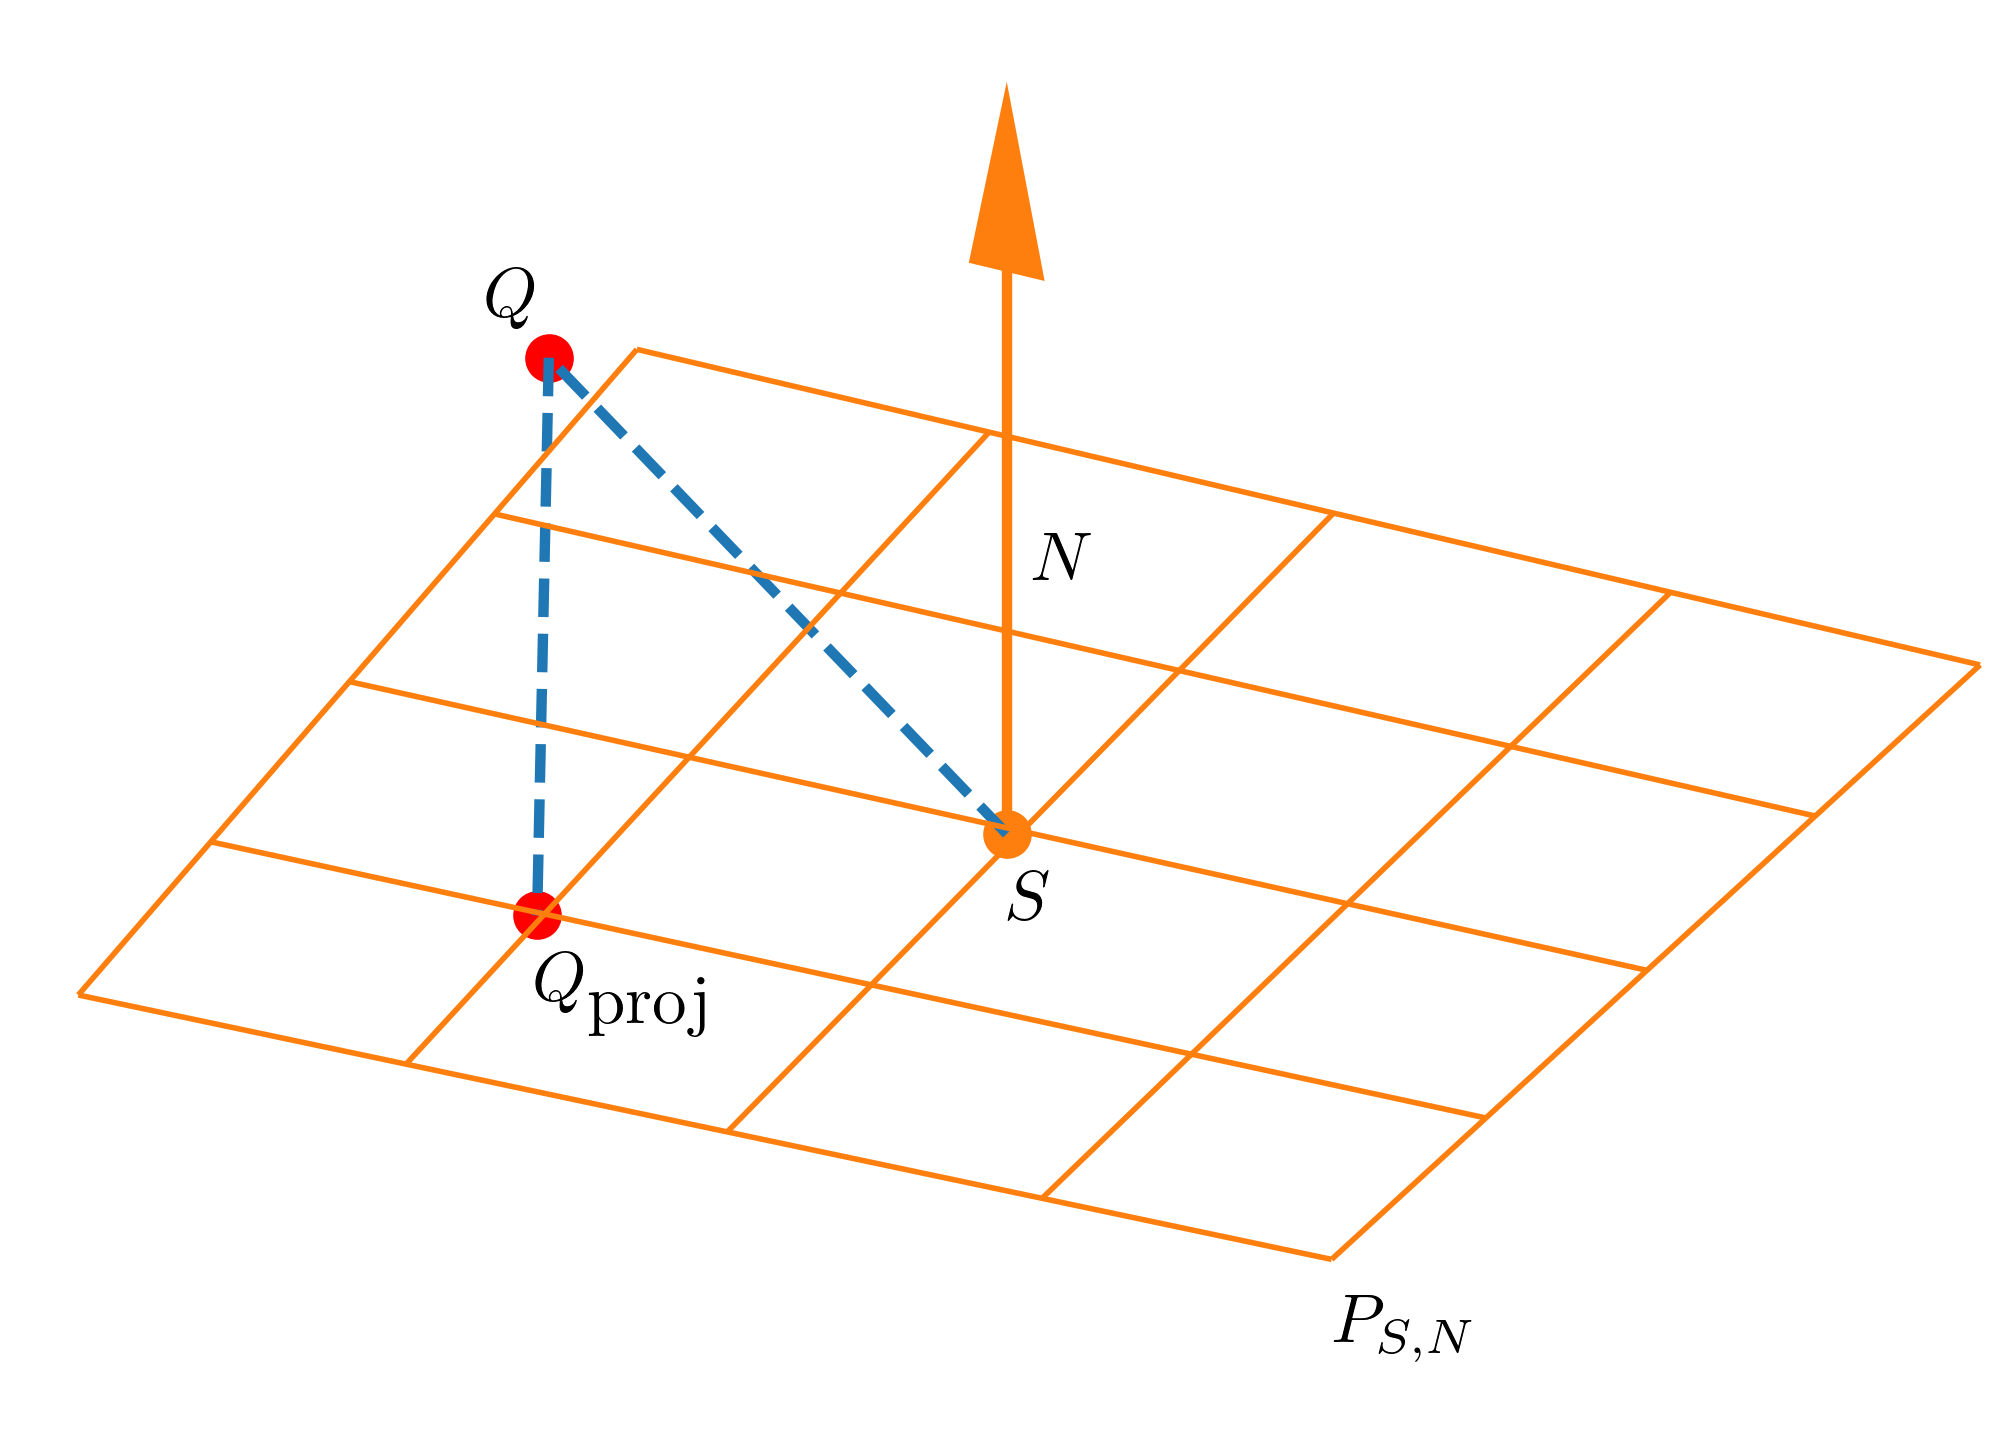
\includegraphics[width=0.4\textwidth]{../python/surfacePlaneIntersection3_cropped.png}
		\caption{Projection of a point onto a plane as described by Theorem \ref{thm:planeprojection}.}
	\end{figure}

	In linear algebra, it is often the case that a plane is defined by a support vector and two direction vectors. In CAD it is instead commonplace to use the pair $(S,N)$ of support vector and normal vector. The normal vector is perpendicular to the two direction vectors of the plane. It should be noted that planes, which are two-dimensional affine subspace of $\mathbb{R}^d$, can only be described that way in the case $d = 3$. In our algorithm, the normal vector notation will prove helpful in combination with the cross product.

	\begin{definition}
		The cross product of two vectors $A, B \in \mathbb{R}^3$ is given by
			$$ A \times B := ||A|| \, ||B|| \, \sin(\theta) \, N,$$
		where $\theta$ is the angle between $A$ and $B$ and $A, B \perp N$ with $||N|| = 1$. Here, $||\cdot||$ is the Euclidean norm of a vector. If $A$ and $B$ are parallel, then $A \times B = 0$
	\end{definition}

	The cross product maps two vectors $A, B$ onto another vector $C$. If $A$ and $B$ are not parallel to each other, the set $\{A,B,C\}$ is a basis of $\mathbb{R}^3$. In other words, the cross product maps to a vector that is perpendicular to the two input vectors.

	\begin{theorem}\label{thm:planeequivalence}
		Let $S \in \mathbb{R}^3$ a support vector and $A, B \in \mathbb{R}^3$ two non-parallel direction vectors. Then the plane $\tilde P = \{S + tA + sB : t, s \in \mathbb{R}\}$ can be written as $P_{S,N}$ with 
			$$ N := \frac{A \times B}{||A \times B||}. $$
	\end{theorem}
	\begin{proof}
		Let $X \in \tilde P$. Then
			$$X - S \; \in \; \tilde P - S = \{tA+sB : t,s \in \mathbb{R}\}.$$
		But then because $A, B \perp N$ we have $X-S \in P_{0,N}$, where $0$ is the null vector. Now, 
			$$ X-S+S = X \in P_{0,N} + S = P_{S,N}.$$
	\end{proof}

	As Theorem \ref{thm:planeequivalence} shows, the notation using the pair $(S,N)$ is valid. Given a parametric surface $\beta(u,v)$ with $(u,v) \in [0,1]^2$, we can construct a plane that is tangent to $\beta(u, v)$ for all $(u,v) \in [0,1]^2$ by using the $u$ and $v$ gradients of $\beta$ and taking their cross product. This yields the normal vector of the tangent plane. The support vector of the plane is just equal to the point $\beta(u,v)$. We make the following definition.

	\begin{definition}\label{def:tangentplanenormal}
		Let $\beta(u,v)$ with $(u,v) \in [0,1]^2$ be a parametric surface that is differentiable in $u$ and $v$. Then the tangent plane of $\beta$ at $(u, v \in [0,1]^2$ is given by the plane
			$$T_{\beta}(u, v) := P_{\beta(u,v), N_{\beta}(u,v)},$$
		where 
			$$N_{\beta}(u,v) := \frac{\nabla_u \beta(u,v) \times \nabla_v \beta(u,v)}{||\nabla_u \beta(u,v) \times \nabla_v \beta(u,v)||}$$
		is the normal vector of the surface $\beta$ at $(u, v)$.
	\end{definition}

	In this section (and in CoolingGen), the surface $\beta(u,v)$ is always differentiable in $u$ and $v$. Suppose we want to intersect the plane $P_{S,N}$ with the parametric surface $\beta(u,v)$ for $(u,v) \in [0,1]^2$. If the surface and the plane do intersect in some point, there exists $(u^{(0)}, v^{(0)}) \in [0,1]^2$ such that $S = \beta(u^{(0)}, v^{(0)})$ is a valid representation for the support vector. If we know such a $(u^{(0)}, v^{(0)})$ a priori, we can find points in the neighborhood of $(u^{(0)}, v^{(0)})$ that also lie in the plane.

	To find a neighboring point, we find the line of intersection $L^{(0)}$ of the tangent plane $T_{\beta}(u^{(0)}, v^{(0)})$ and the target plane $P_{S,N} = P_{\beta(u^{(0)}, v^{(0)}), N}$. Using the normal notation of the planes and the intersection parameter pair $(u^{(0)}, v^{(0)})$, we can easily do this using the following theorem.

	\begin{theorem}
		Let $P_{S, N_1}$ and $P_{S, N_2}$ be two planes with $N_1$ and $N_2$ not parallel. Then
			$$ P_{S, N_1} \cap P_{S, N_2} = L_{S, S+N}(-\infty, \infty), $$
		where $N = \frac{N_1 \times N_2}{|| N_1 \times N_2 ||}$ and $L_{S,S+N}(-\infty, \infty)$ is the line through $S$ and $S+N$. 
	\end{theorem}
	\begin{proof}
		Let $t \in \mathbb{R}$. Notice that $tN \perp N_1$ and $tN \perp N_2$. Therefore, $tN \in P_{0, N_1} \cap P_{0, N_2}$, which is equivalent to $S+tN \in P_{S, N_1} \cap P_{S, N_2}$. But $S+tN = (1-t)S + t(S+N) = L_{S,S+N}(t)$ according to Definition \ref{def:linesegdef}.
	\end{proof}

	The tangent intersection line for the intersection parameters $(u^{(0)}, v^{(0)})$ is equal to
		$$ L^{(0)}(t) = \beta(u^{(0)}, v^{(0)}) + t \cdot \left(\frac{N_{\beta}(u^{(0)}, v^{(0)}) \times N}{||N_{\beta}(u^{(0)}, v^{(0)}) \times N||}\right)$$
	for $t \in \mathbb{R}$. Using an appropriate step size $\alpha \in \mathbb{R}$, we can project the point $L^{(0)}(\alpha) \in T_{\beta}(u^{(0)}, v^{(0)}) \cap P_{\beta(u^{(0)}, v^{(0)}), N}$ onto the surface $\beta$ using the methods from Section \ref{subsec:pointproj} to acquire a candidate for the point $\beta(u^{(1)}, v^{(1)})$. If this point lies outside of the plane $P_{S,N}$, we discard the point, choose a step size less than $\alpha$ and repeat the process. Numerically, we accept a candidate if it is within $\epsilon$-distance of the plane $P_{\beta(u^{(0)}, v^{(0)}), N}$ for a small value of $\epsilon > 0$. If $\beta(u^{(1)}, v^{(1)})$ has been found, we repeat this process to find $\beta(u^{(2)}, v^{(2)})$. To do this, we construct $L^{(1)}$ by intersecting $P_{S,N}$ and $T_{\beta}(u^{(1)}, v^{(1)})$ and project $L^{(1)}(\alpha)$ onto $\beta$. We can repeat this iteration step until $|\alpha| < \alpha_0$ for some $\alpha_0 > 0$. If this condition is satisfied, we return the list of the $n$ parameters of intersection, which we can write as $L = \{(u^{(i)}, v^{(i)}): i \in \{1,2,...,n\}\}$.

	\begin{algorithm}[H]
	\begin{algorithmic}[1]
		\Input
			\Desc{$\alpha > \alpha_0$}{\phantom{aa} step size and minimum step size}
			\Desc{$\xi < 1$}{\phantom{aa} step size scaling factor}
			\Desc{$\epsilon$}{\phantom{aa} absolute tolerance}
		\EndInput
		\Output
			\Desc{$\{(u^{(i)}, v^{(i)}) : i \in \{1, 2, ..., n\}\}$ }{\phantom{aa} set of points on the intersection}
		\EndOutput

		\caption{Surface Plane Intersection}\label{alg:surfplaneintersection}
		\Procedure{intersectSurfacePlane}{$\beta, S, N, (u^{(0)}, v^{(0)})$}
			\State $L \gets$ list containing only $(u^{(0)}, v^{(0)})$
			\While {$|\alpha| > |\alpha_0|$}
				\State $(u,v) \gets$ last entry in $L$
				\State $M \gets \left(\frac{N_{\beta}(u, v) \times N}{||N_{\beta}(u, v) \times N||}\right)$
				\State $P \gets \beta(u,v) + \alpha M$
				\State $u_\textrm{proj}, v_\textrm{proj} = \textrm{pointProjection}(\beta, P)$
				\If {$D(\beta(u_\textrm{proj}, v_\textrm{proj}), P_{S,N}) > \epsilon$}
					$\alpha \gets \xi\alpha$
				\Else {} append $(u_\textrm{proj}, v_\textrm{proj})$ to $L$
				\EndIf
			\EndWhile
			\State \Return $L$
		\EndProcedure
	\end{algorithmic}
	\end{algorithm}

	After successfully running Algorithm \ref{alg:surfplaneintersection}, we are left with $n$ points which lie on the intersection curve. We interpolate between these points using NURBS (see \cite{Piegl1997}). If necessary, the control points of the NURBS curve can then be projected onto the plane $P_{S,N}$ to ensure that the curve is planar. This scheme proves useful for CoolingGen, because a start parameter pair $(u^{(0)}, v^{(0)})$ is practically always known in this context. Otherwise, a start point can be found using the ray marching technique, which was discussed in Section \ref{subsec:raymarching}.

	\begin{figure}[H]
		\centering
		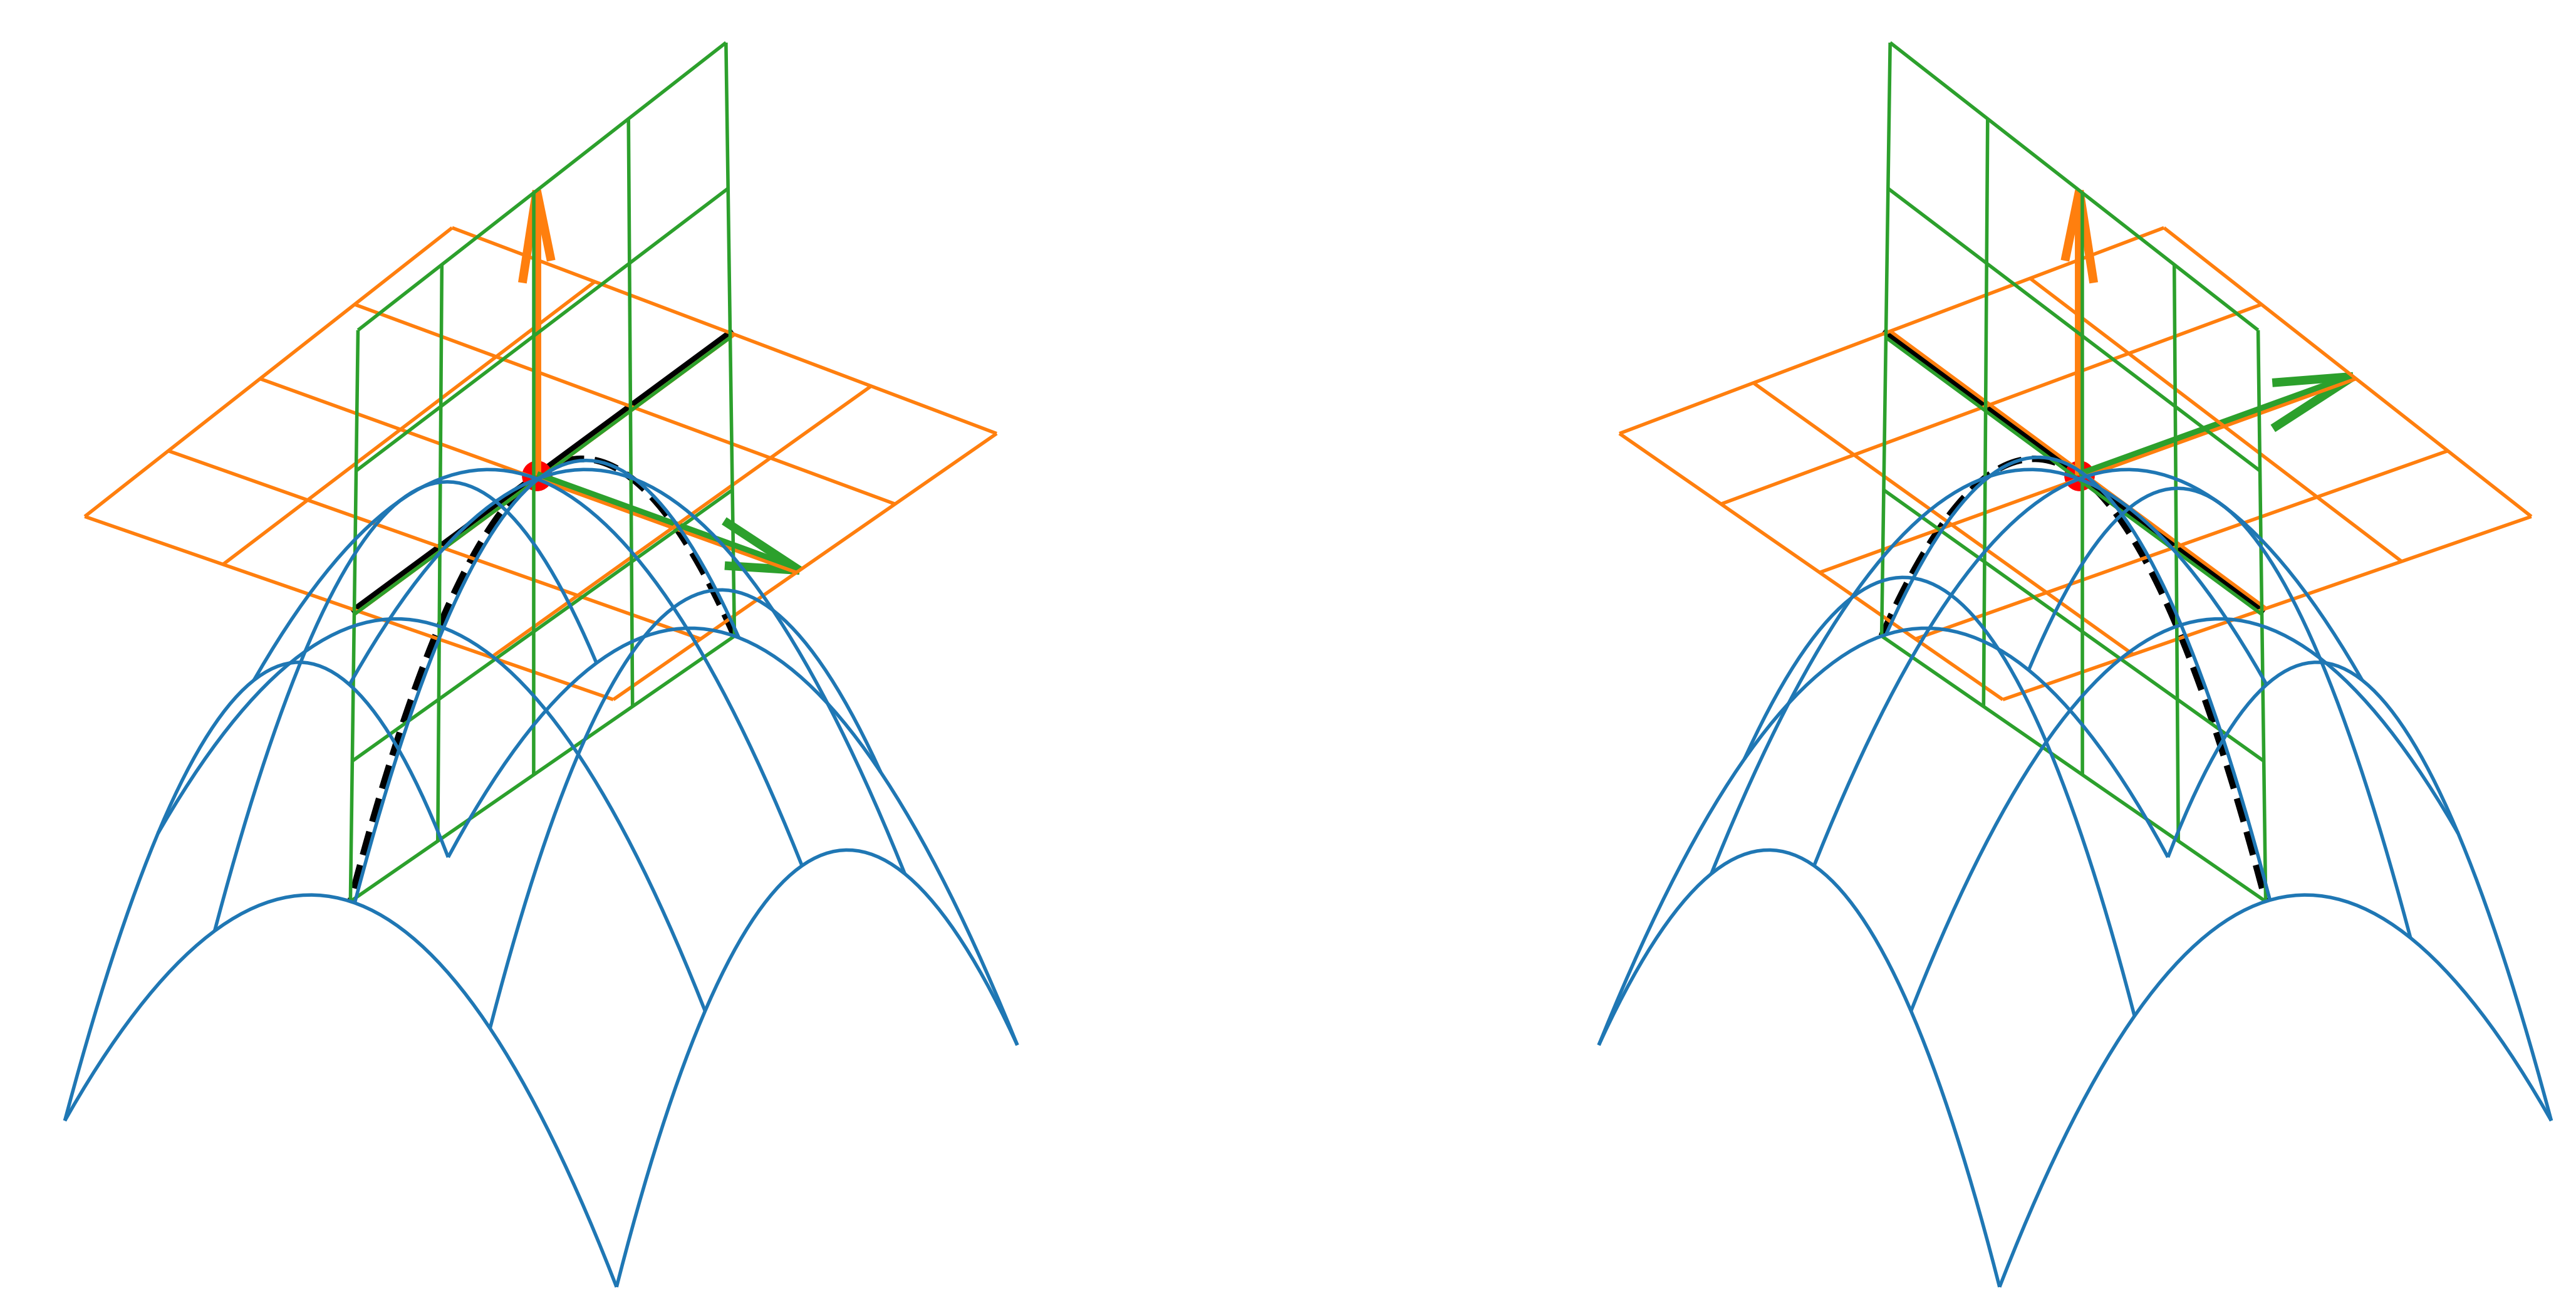
\includegraphics[width=.8\textwidth]{../python/surfacePlaneIntersection2_cropped.png}
		\caption{Intersection of a surface $\beta$ (blue) with the plane $P_{S,N}$ (green). The intersection point $\beta(u^{(0)}, v^{(0)})$ is represented by the red dot. We intersect the tangent plane (orange) of $\beta$ at $(u^{(0)}, v^{(0)})$ with $P_{S,N}$, yielding the line $L^{(0)}$ (black). Near the intersection point, $L^{(0)}$ and the true solution (black dashed curve) are close. The arrows represent the normal vectors.}
		\label{fig:planeintersectionline}
	\end{figure}

\subsection{Coons Patch}
	Given four parametric boundary curves $c_0(t)$, $c_1(t)$, $d_0(t)$ and $d_1(t)$ for $t \in [0,1]$ with $c_0(0) = d_0(0)$, $c_0(1) = d_1(0)$, $c_1(0) = d_0(1)$ and $c_1(1) = d_1(1)$ we can construct an intermediate parametric surface $\mathfrak{C}$ by using linear interpolation on pairs $c_0, c_1$ and $d_0, d_1$ and bilinear interpolation the corner points $c_0(0), c_0(1), c_1(0), c_1(1)$ using bilinear blending, in other words
	\begin{align*}
		\mathfrak{C}(u,v) 	&= (1-v)\,c_0(u) + v\,c_1(u) \\
				&+ (1-u)\,d_0(v) + u\,d_1(v) \\
				&- (1-u)(1-v)\,c_0(0) - u(1-v)\,c_0(1)(1) - (1-u)v\,c_1(0) - uv\,c_1(1),
	\end{align*}
	where $(u,v) \in [0,1]^2$. Such a surface is called a Coons patch \cite{Coons1967}. 

	\begin{figure}[H]
		\centering
		\includesvg[width=0.7\textwidth]{../python/coonsPatch}
		\caption{Example of a Coons patch $\mathfrak{C}$.}
	\end{figure}

\chapter{Jet Engine Specific Methods}\label{chap:jetenginespecifics}
	CoolingGen creates geometries which lie inside a blade or vane surface $B(u,v)$, which is an output of BladeGen, a tool developed by the DLR specifically for the design of blade and vane surfaces. $B(u,v)$ is closed in $u$-direction. For a given $u$, increasing $v$ yields a further distance from the turbines hub. Because of rotational symmetry of the turbine, it is convenient to describe these geometries in cylindrical coordinates. The transformation from Cartesian coordinates to cylindrical coordinates in this case is given by the map
		$$ Z: (x,y,z) \mapsto (x, r, \theta), $$
	where $\theta = \arctantwo(y, z)$ is the circumferential angle and $\sqrt{y^2+z^2}$ is the distance from the turbine hub. This transformation is invertible.

	\begin{figure}[H]
		\centering
		\begin{subfigure}{.49\textwidth}
			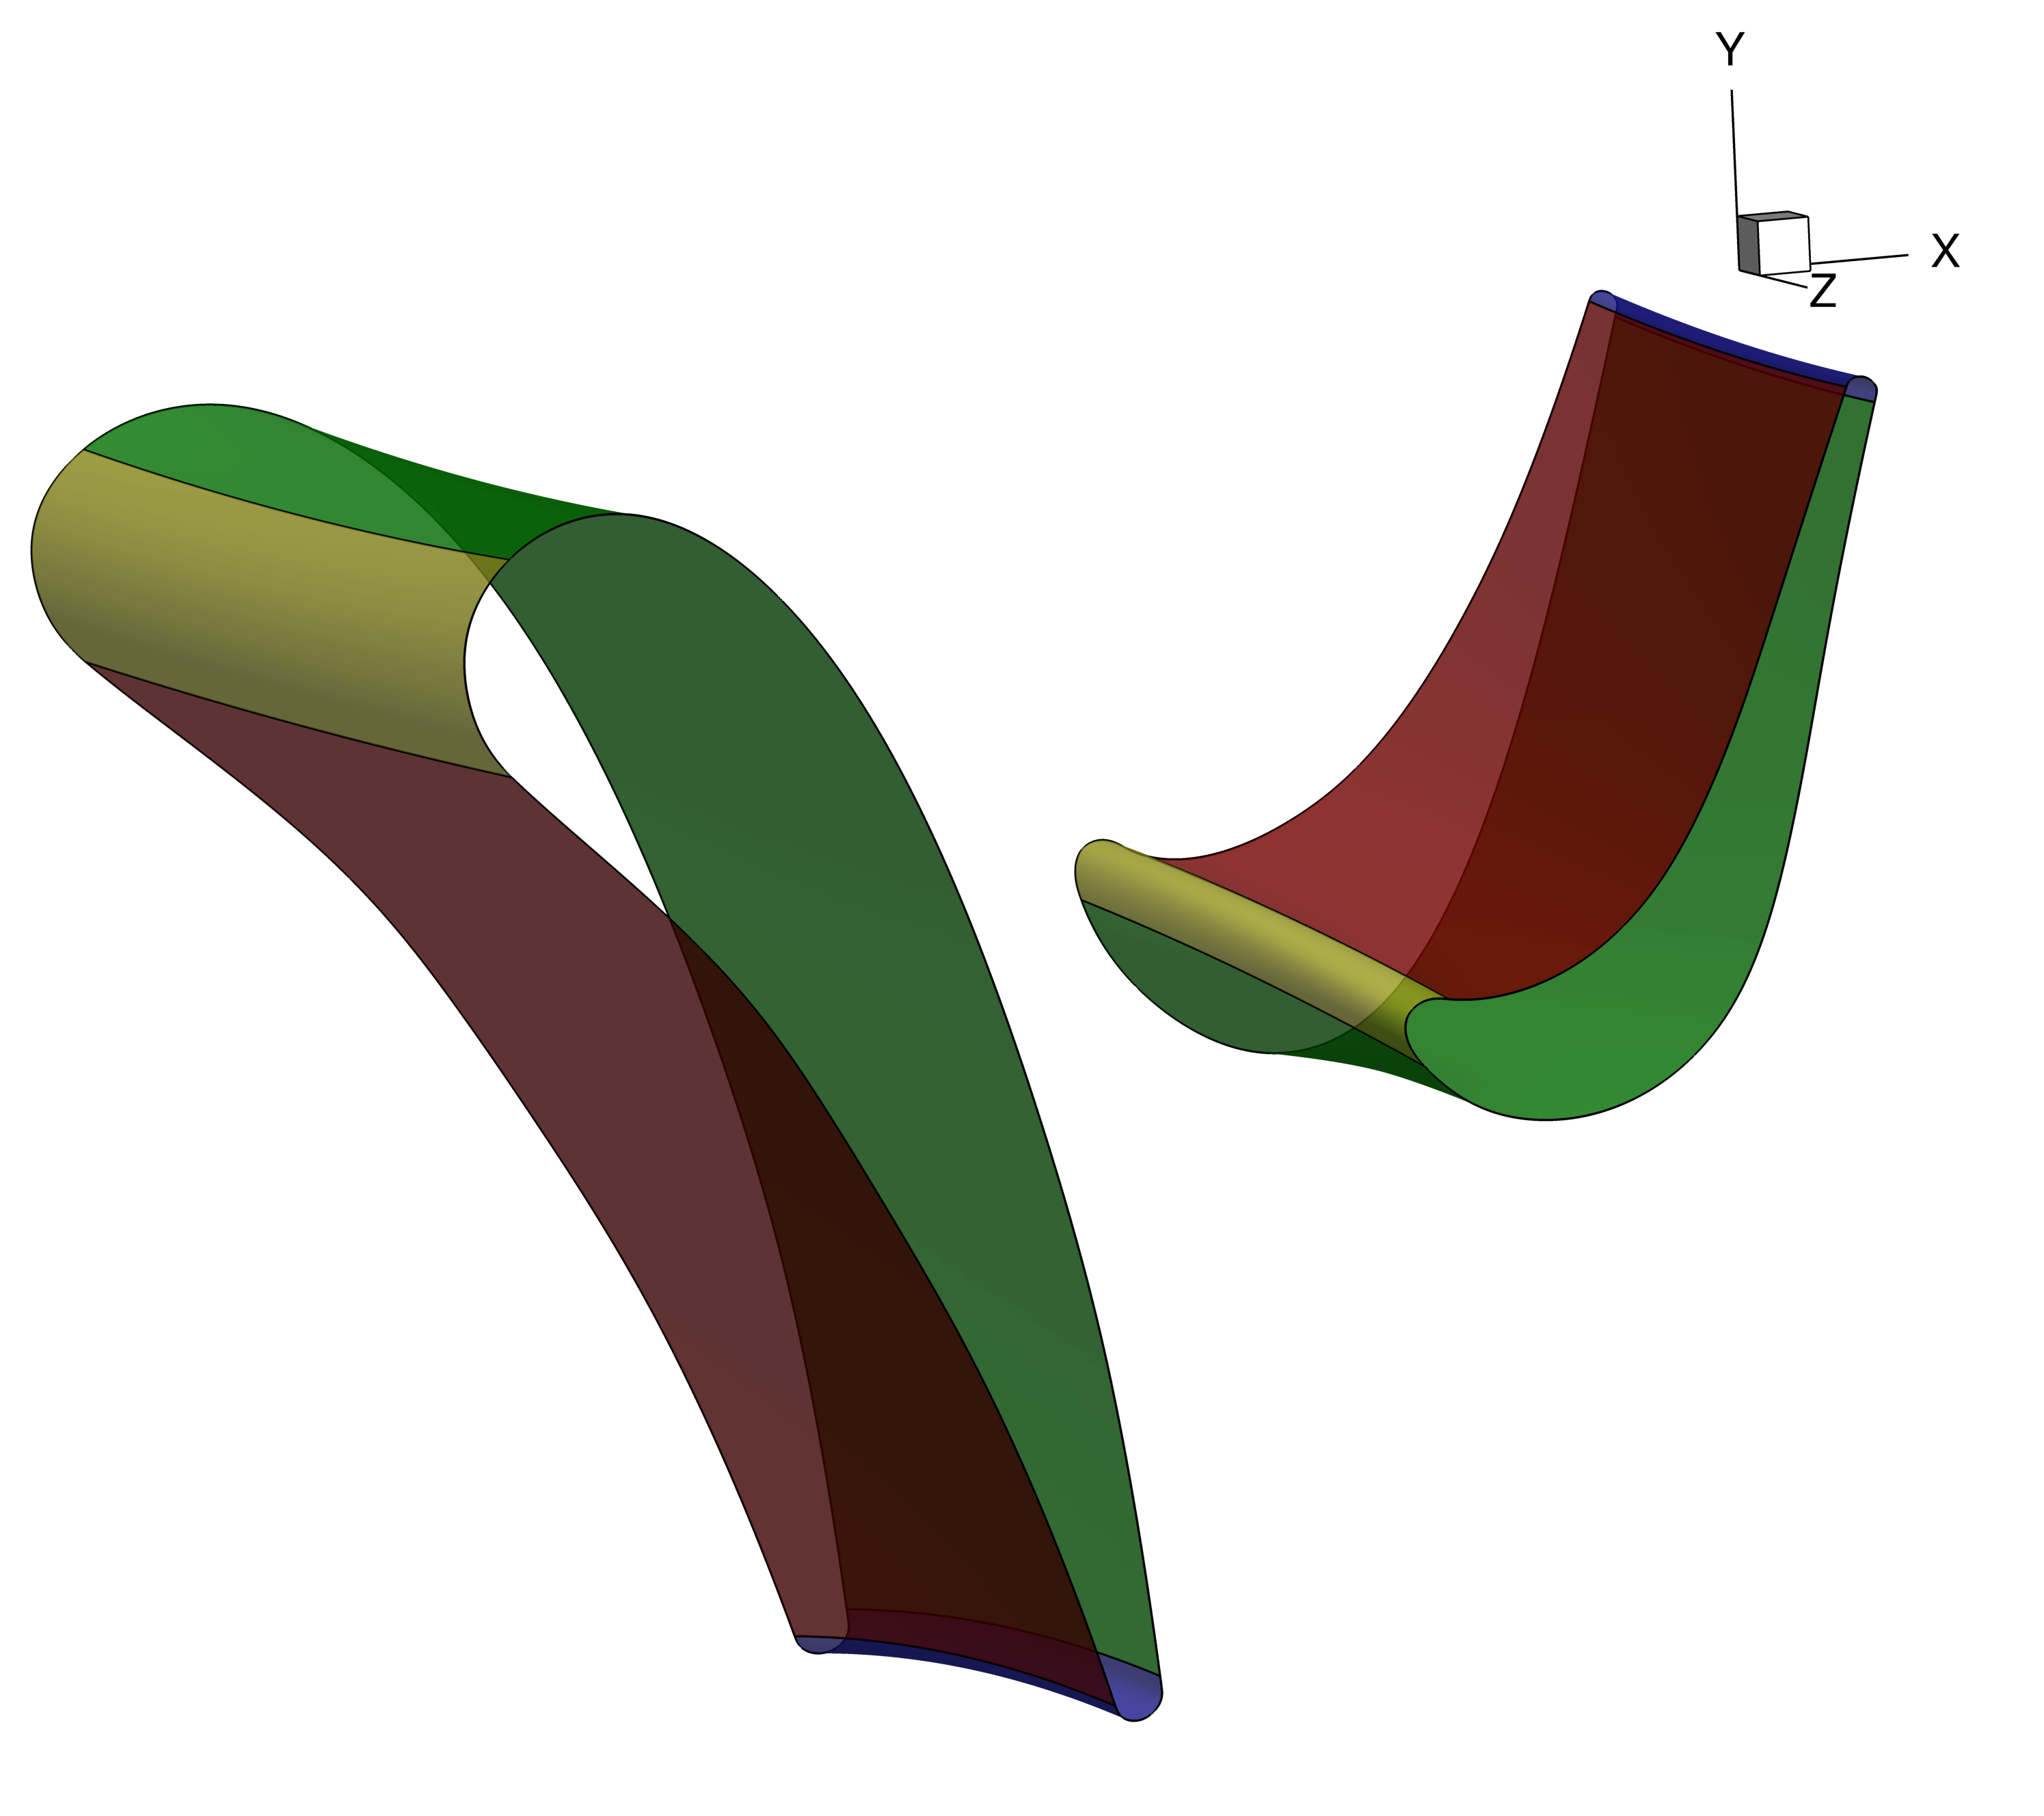
\includegraphics[width=\textwidth]{../tec/rotor_stator/11.png}
			\caption{View on pressure side.}
		\end{subfigure}
		\begin{subfigure}{.49\textwidth}
			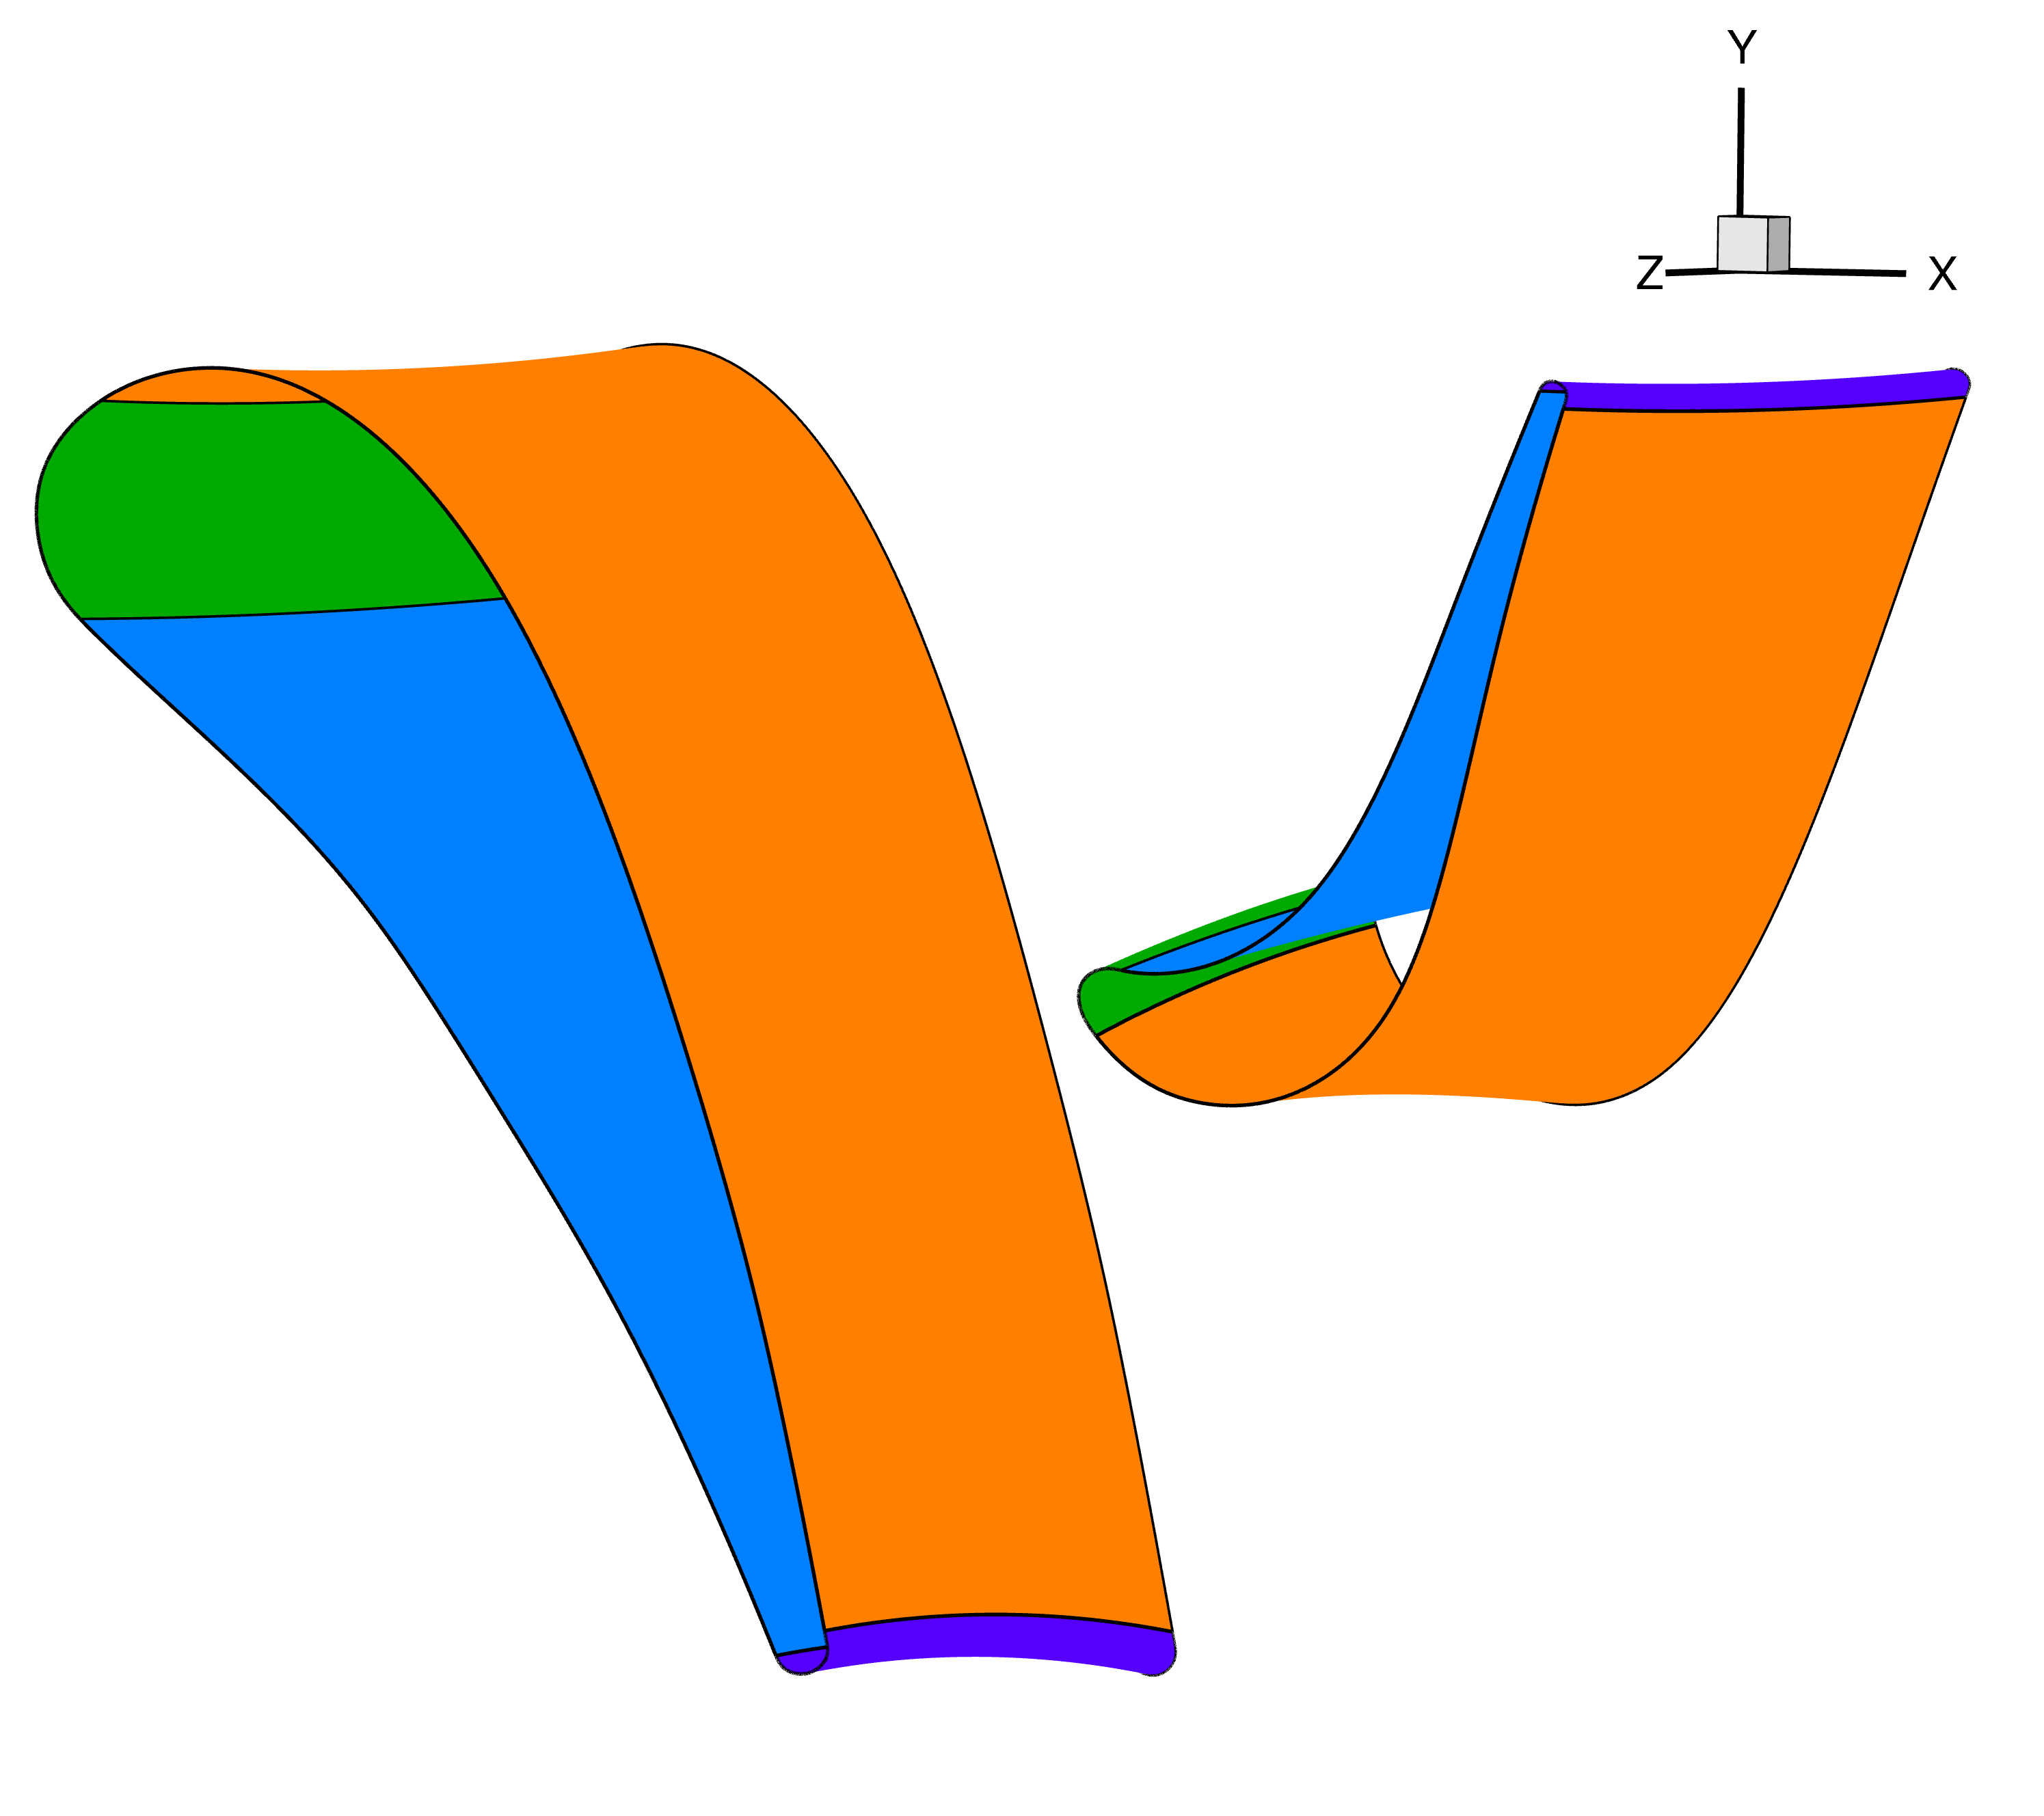
\includegraphics[width=\textwidth]{../tec/rotor_stator/12.png}
			\caption{View on suction side.	}
		\end{subfigure}
		\caption{In (a) and (b), the left is surface represents a stator vane and the right surface represents a rotor blade. The blade has a named partitioning into the leading edge (green), the pressure side (blue), the suction side (orange) and the trailing edge (purple).}
		\label{fig:rotor_stator}
	\end{figure}

	A distinction is made between two kinds of surfaces: rotor blades and stator vanes. While the rotor blades rotate around the hub, the stator vanes have fixed positions. Furthermore, the blade or vane surface $B(u,v)$ has a named partitioning in $u$-direction into four distinct parts. The leading edge, the suction side, the trailing edge and the pressure side.

\section{The S2 Stream Surface \& Stream Surface Coordinates}\label{sec:mrtheta}
	A stream line is a line that at every point is tangential to the velocity vector field of the flow of the fluid. Its generalization, the stream surface, describes a surface with the same property. The flow in a turbine can be described by a generalization of the stream surface. When designing turbine blades or vanes, it is common practice to describe the flow in two families of stream surfaces. These surfaces are called $S_1$ and $S_2$. The $S_1$ surfaces, also known as \emph{blade-to-blade} surfaces, describe the flow behavior between individual blade (or vane) sections, whereas their counterpart, the $S_2$ surfaces, which are also known as \emph{meridional} surfaces, describe the flow in the axial direction \cite{Wu1952}.

	\begin{figure}[H]
		\centering
		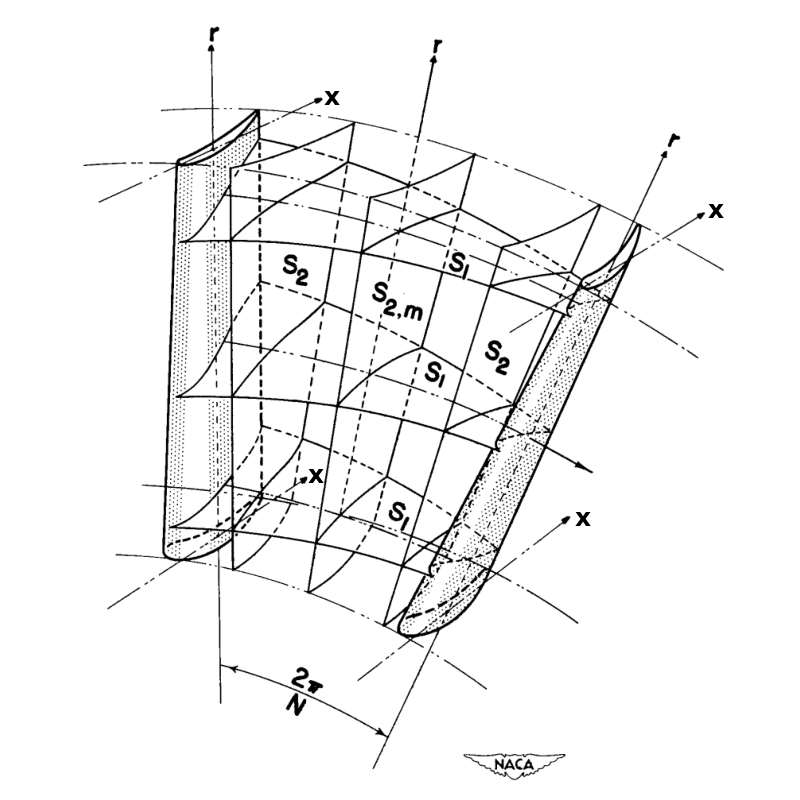
\includegraphics[width=.5\textwidth]{../assets/renamed_wu_naca_s2.png}
		\caption{Example $S_1$ and $S_2$ surfaces of a turbomachine from \cite{Wu1952}.}
	\end{figure}
	
	Each $S_2$ surface is a parametric surface and therefore a map
		$$s(u,v) : [0,1]^2 \rightarrow \mathbb{R}^3, \quad (u,v) \mapsto (x, r, m),$$
	where $x$ is the axial coordinate, $r = \sqrt{y^2+z^2}$ the distance from the turbine hub and 
		$$m(u,v) = \int_0^u \sqrt{x(t,v)^2 + r(t,v)^2} \; \textrm{dt}$$
	is the $v$-isoparametric arc length of the stream surface. To design the blades (and vanes) for turbomachinery, BladeGen and CoolingGen make use of a certain $S_2$ surface, the so called $S_{2,m}$ surface. This surface lies midway between two blades \cite{Wu1952}. Each stream line described by $S_{2,m}$ can then be written as $v$-isoparametric curve $S_{2,m}(\cdot, v)$.

	By intersecting the transformed $u$-isoparametric curves $Z(B(u,\cdot))$ of the blade (or vane) with each such stream line $S_{2,m}(\cdot, v)$ in their first two arguments $(x,r)$, we can construct a curve
		$$ B^{(v)}_\textrm{stream}(u) = (m, r\theta),$$
	where $m$ is the intersection arc length of $S_{2,m}(\cdot, v)$, $r$ is the intersection distance from the hub and $\theta$ is the intersection circumferential angle. This coordinate system with respect to arc length $m$ and radius-angle product $r\theta$ is a so called \emph{stream surface coordinate system}. Given $v$ and the stream surface, each point $(m, r\theta)$ can bijectively be mapped back onto the respective Cartesian coordinates $(x, y, z)$.

	Since this coordinate transformation produces a set of planar curves for $v_i \in [0,1]$, where $i \in \{1, 2, ..., N\}$, we can use two-dimensional operations on such a set of stream surface curves instead of using three-dimensional operations directly on the Cartesian represented $B(u,v)$. This yields a significant performance boost. The resulting stream surface curves can then be transformed back to the Cartesian coordinate system. Using surface skinning we can interpolate between families of stream surface curves to find a surface (see \cite{Piegl1997}). This approach will be used in the construction of the internal geometries.

\chapter{Results}\label{chap:results}
	In this chapter, we present the construction of different blade and vane cooling geometries using CoolingGen. For this purpose, we require the methods presented in Chapter \ref{chap:methods} and Chapter \ref{chap:jetenginespecifics}. As mentioned before, CoolingGen is capable of producing four distinct types of geometries: channels, film cooling holes, impingement inserts and trailing edge slots. These four types are supported on rotor blades as well as on stator vanes.
 	
	\begin{figure}[H]
		\centering
		\begin{subfigure}{.49\textwidth}
			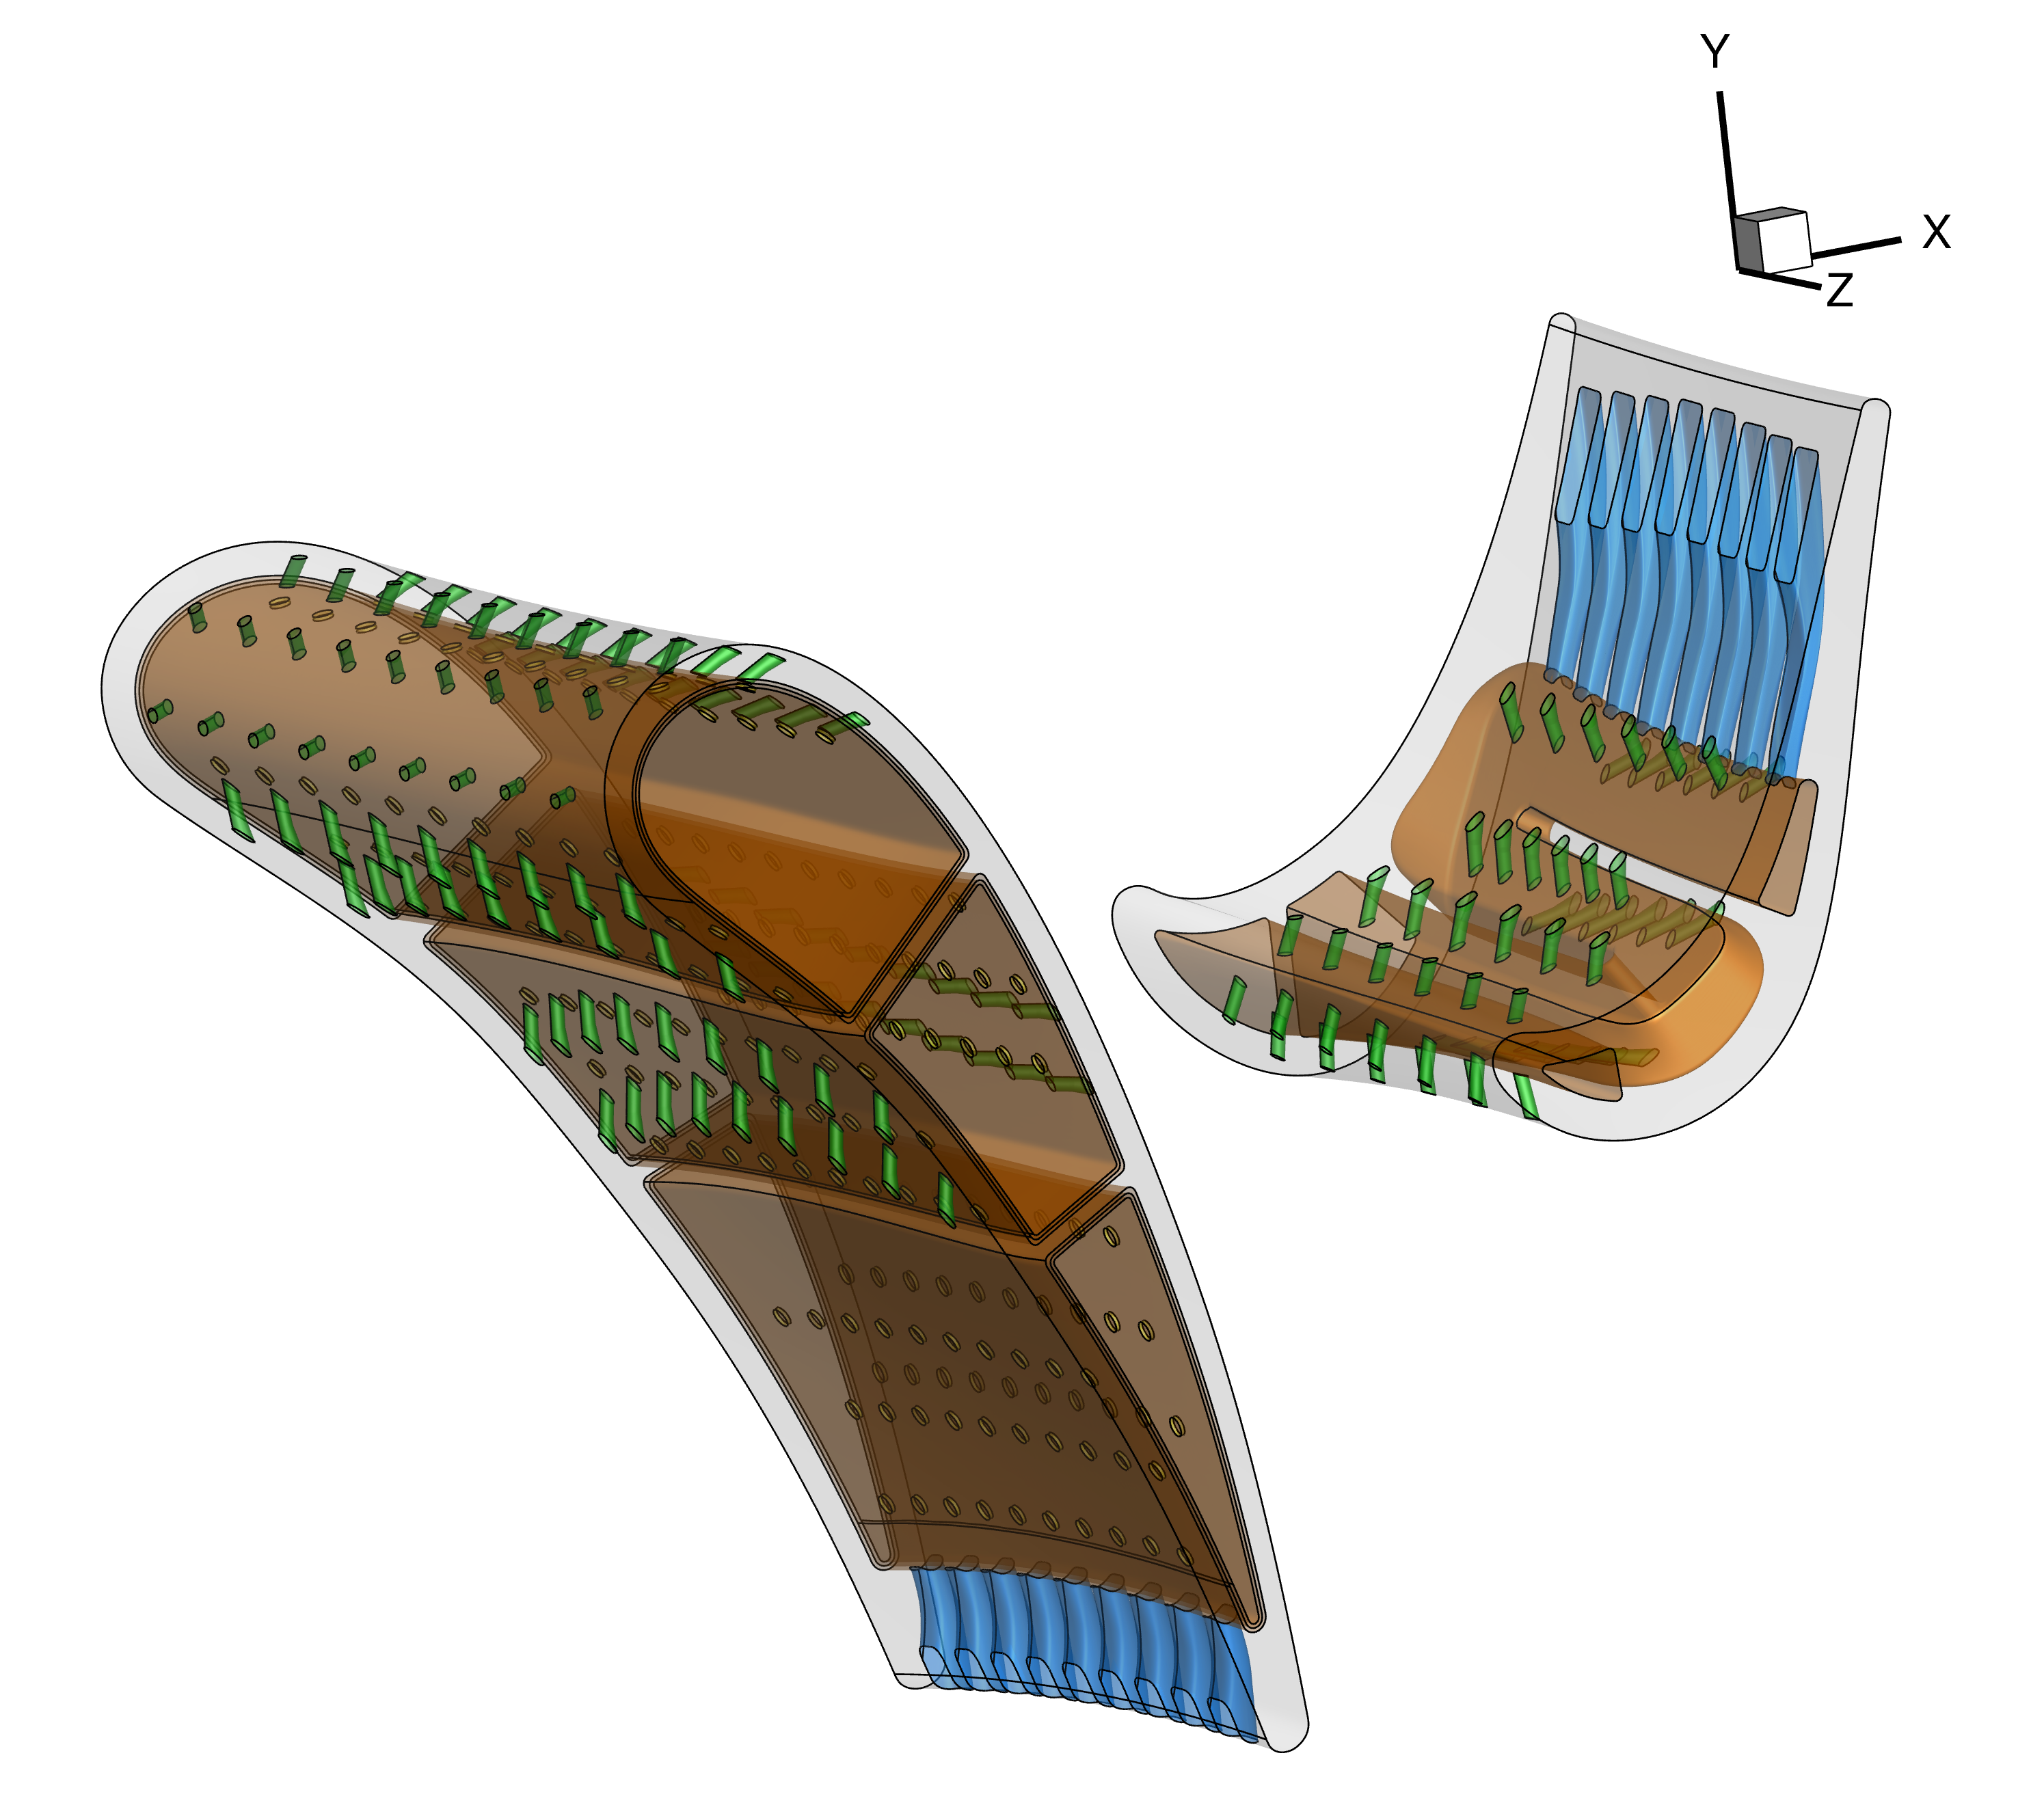
\includegraphics[width=\textwidth]{../tec/complete/60.png}
			\caption{View on pressure side.}
		\end{subfigure}
		\begin{subfigure}{.49\textwidth}
			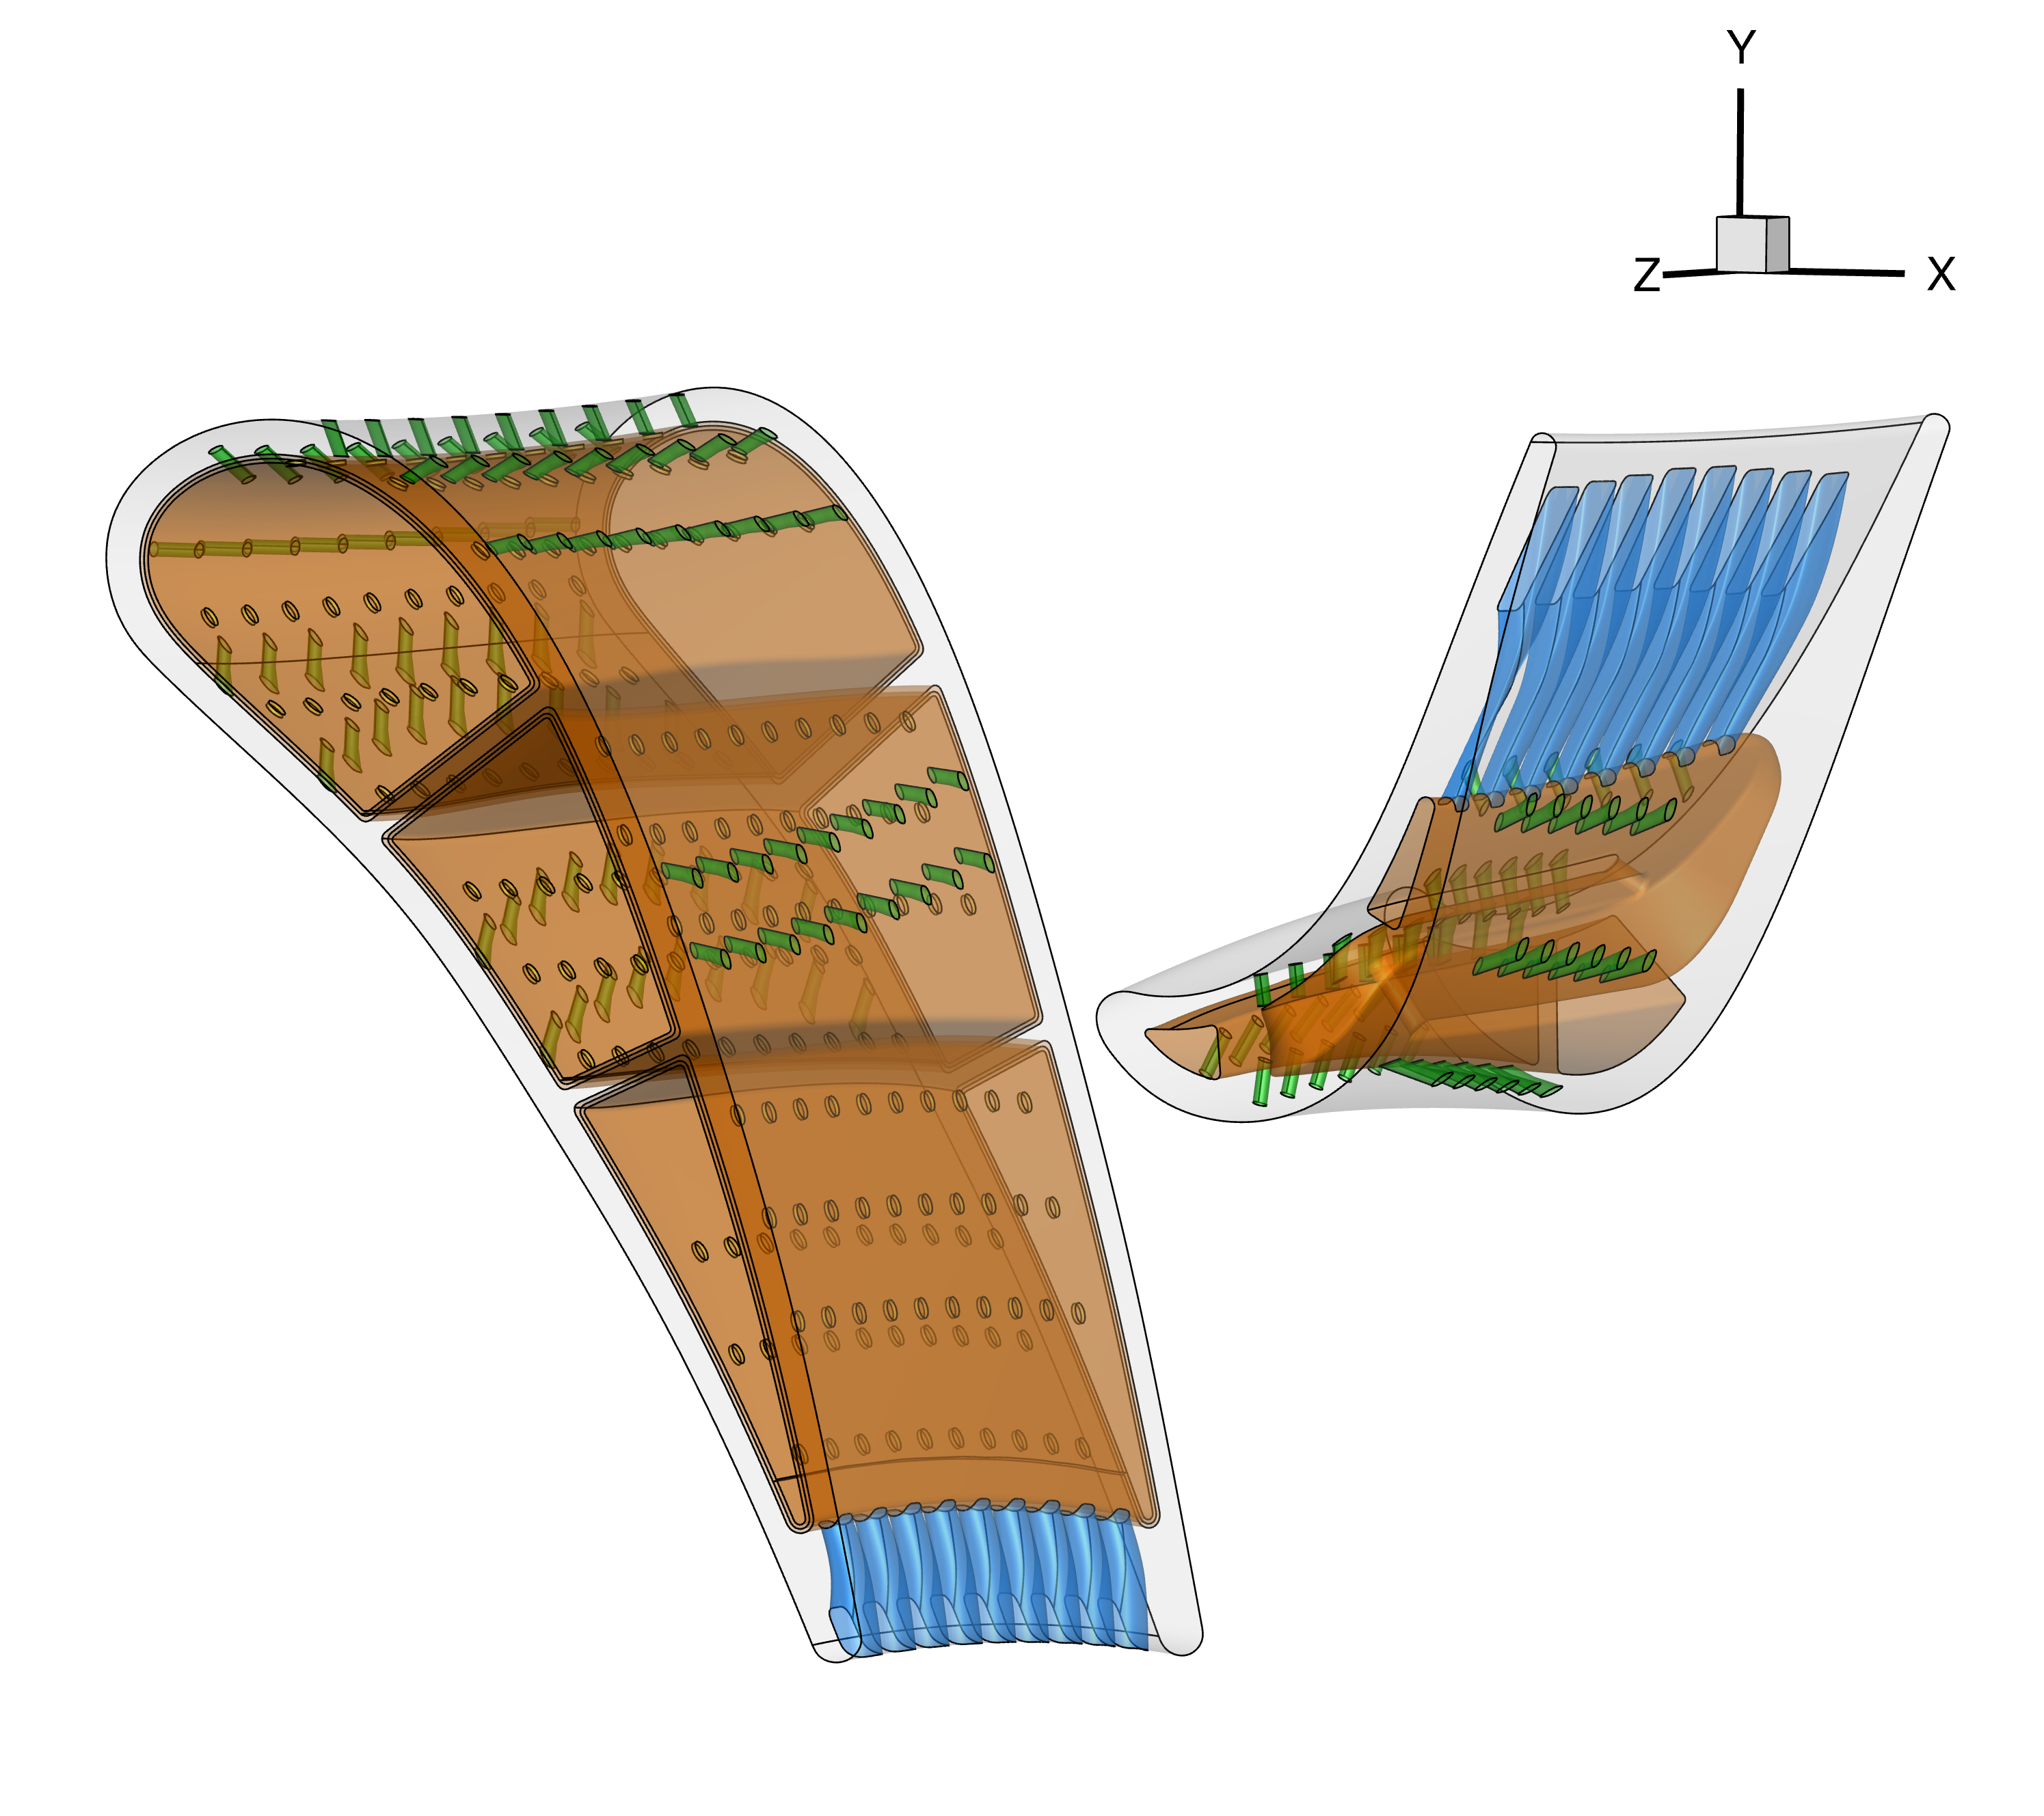
\includegraphics[width=\textwidth]{../tec/complete/61.png}
			\caption{View on suction side.}
		\end{subfigure}
		\begin{subfigure}{.49\textwidth}
			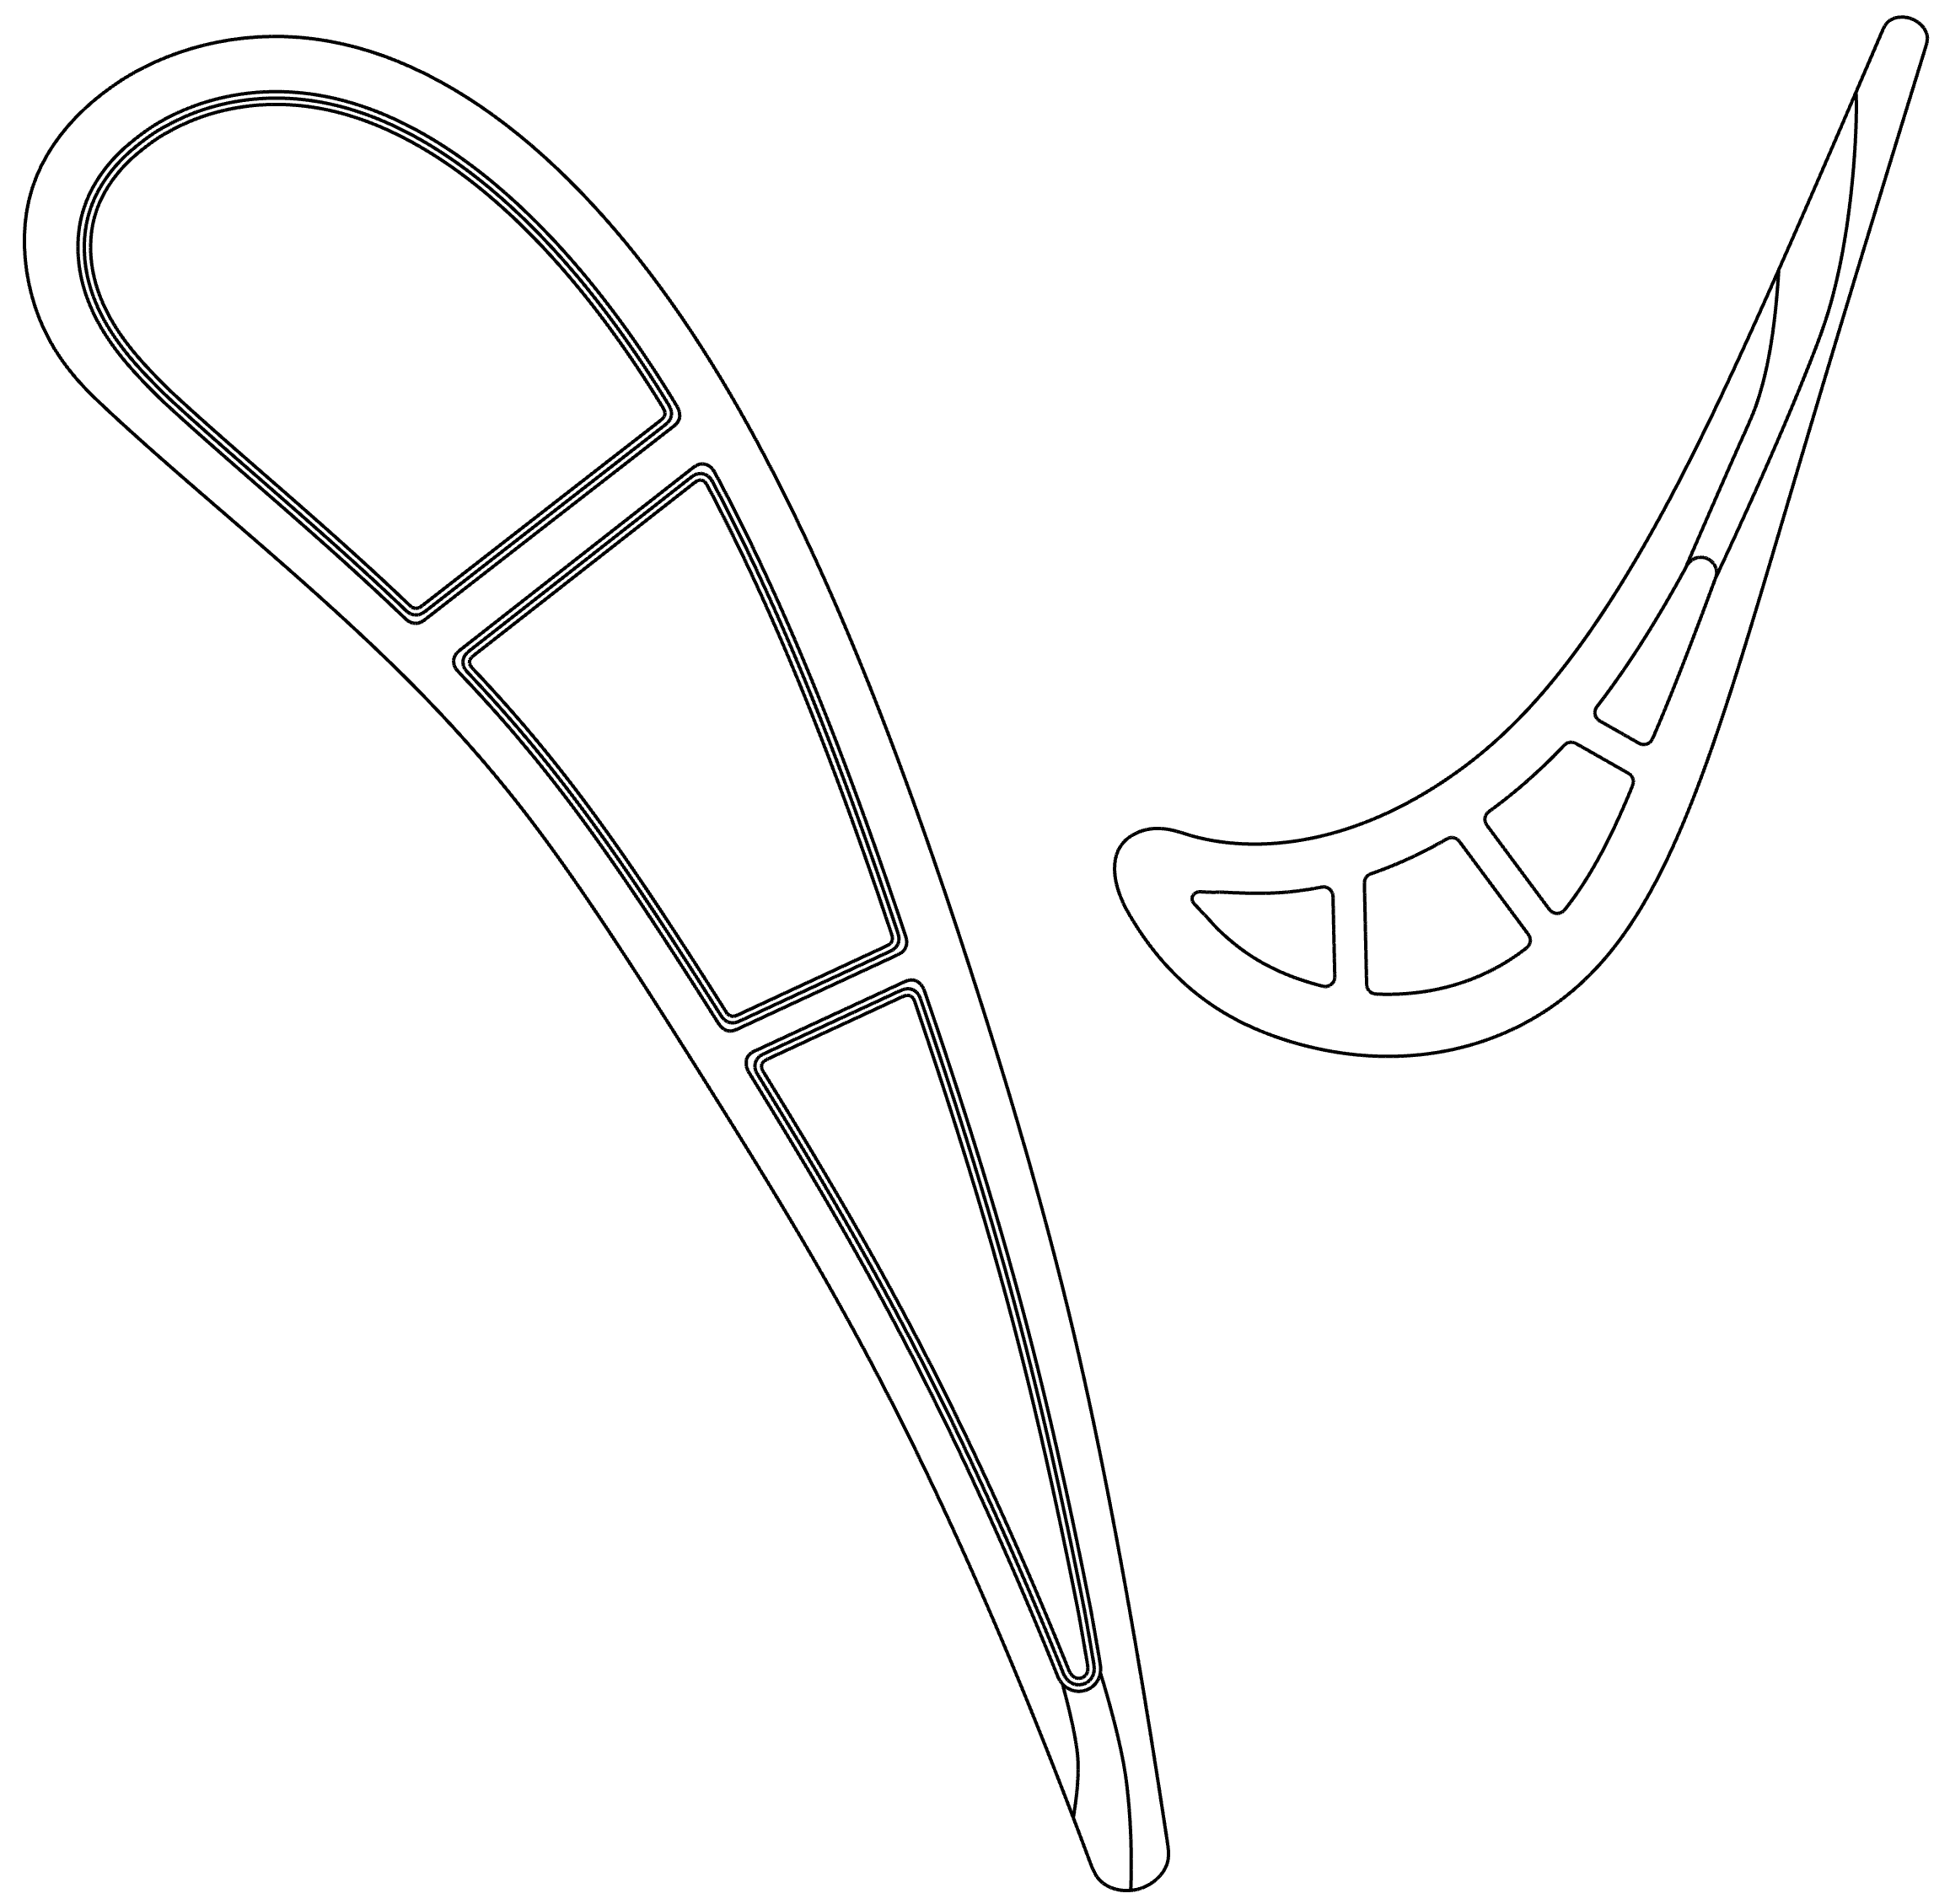
\includegraphics[width=\textwidth]{../tec/complete/003.png}
			\caption{Profile view.}
		\end{subfigure}
		\begin{subfigure}{.49\textwidth}
			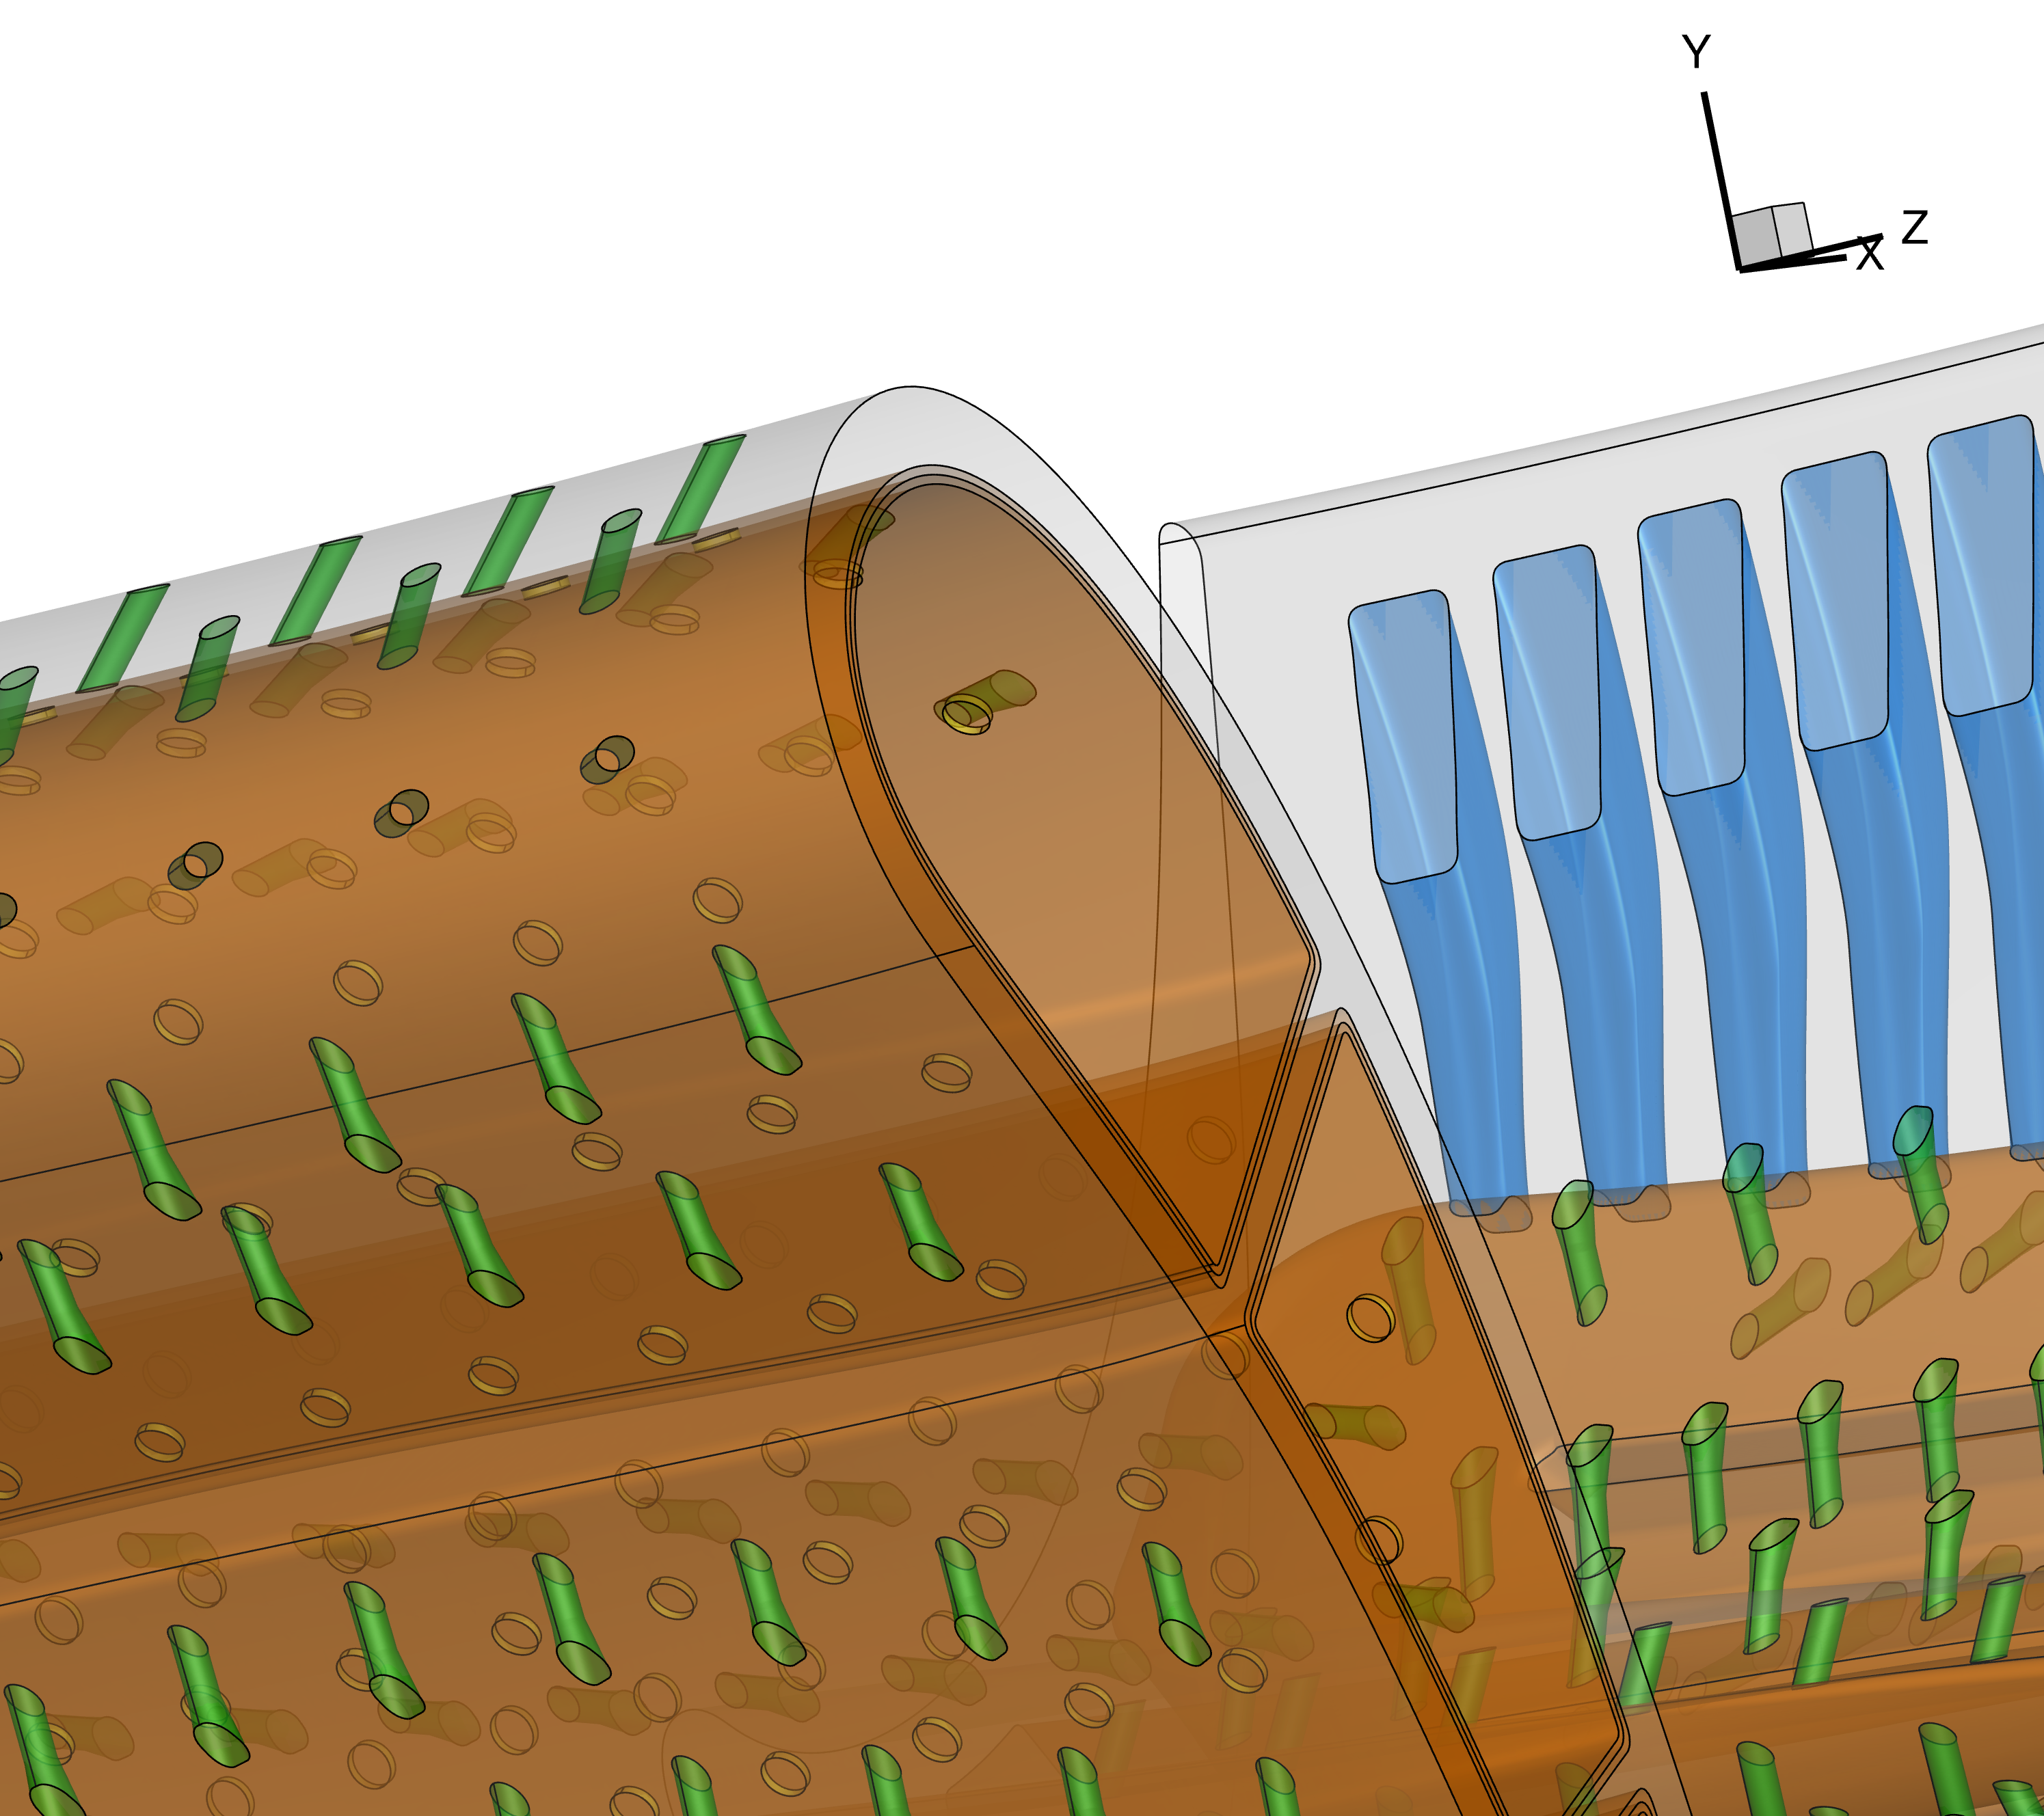
\includegraphics[width=\textwidth]{../tec/complete/80.png}
			\caption{Detailed view.}
		\end{subfigure}		
		\caption{Like Figure \ref{fig:rotor_stator}, but equipped with cooling geometries. The outer orange surfaces are channels. The green surfaces are film cooling holes. The inner orange surfaces are impingement inserts. The short yellow cylindrical surfaces represent the holes inside the impingement inserts. In the detailed view, we can see the impingement insert of the leading edge channel of the stator and the slots on the pressure side of the rotor.}
		\label{fig:results_complete}
	\end{figure}

\section{Channels}
	 For the construction of channels, we distinguish between straight and curved sections of the channel. The straight sections represent hollow bodies that let the coolant pass in $v$-direction of the turbine blade. These sections are called chambers. The curved sections let the coolant pass in $u$-direction of the turbine blade. We call the latter sections turns. Inside turns, the coolant flows between chambers.

	\begin{figure}[H]
		\centering
		\begin{subfigure}{.49\textwidth}
			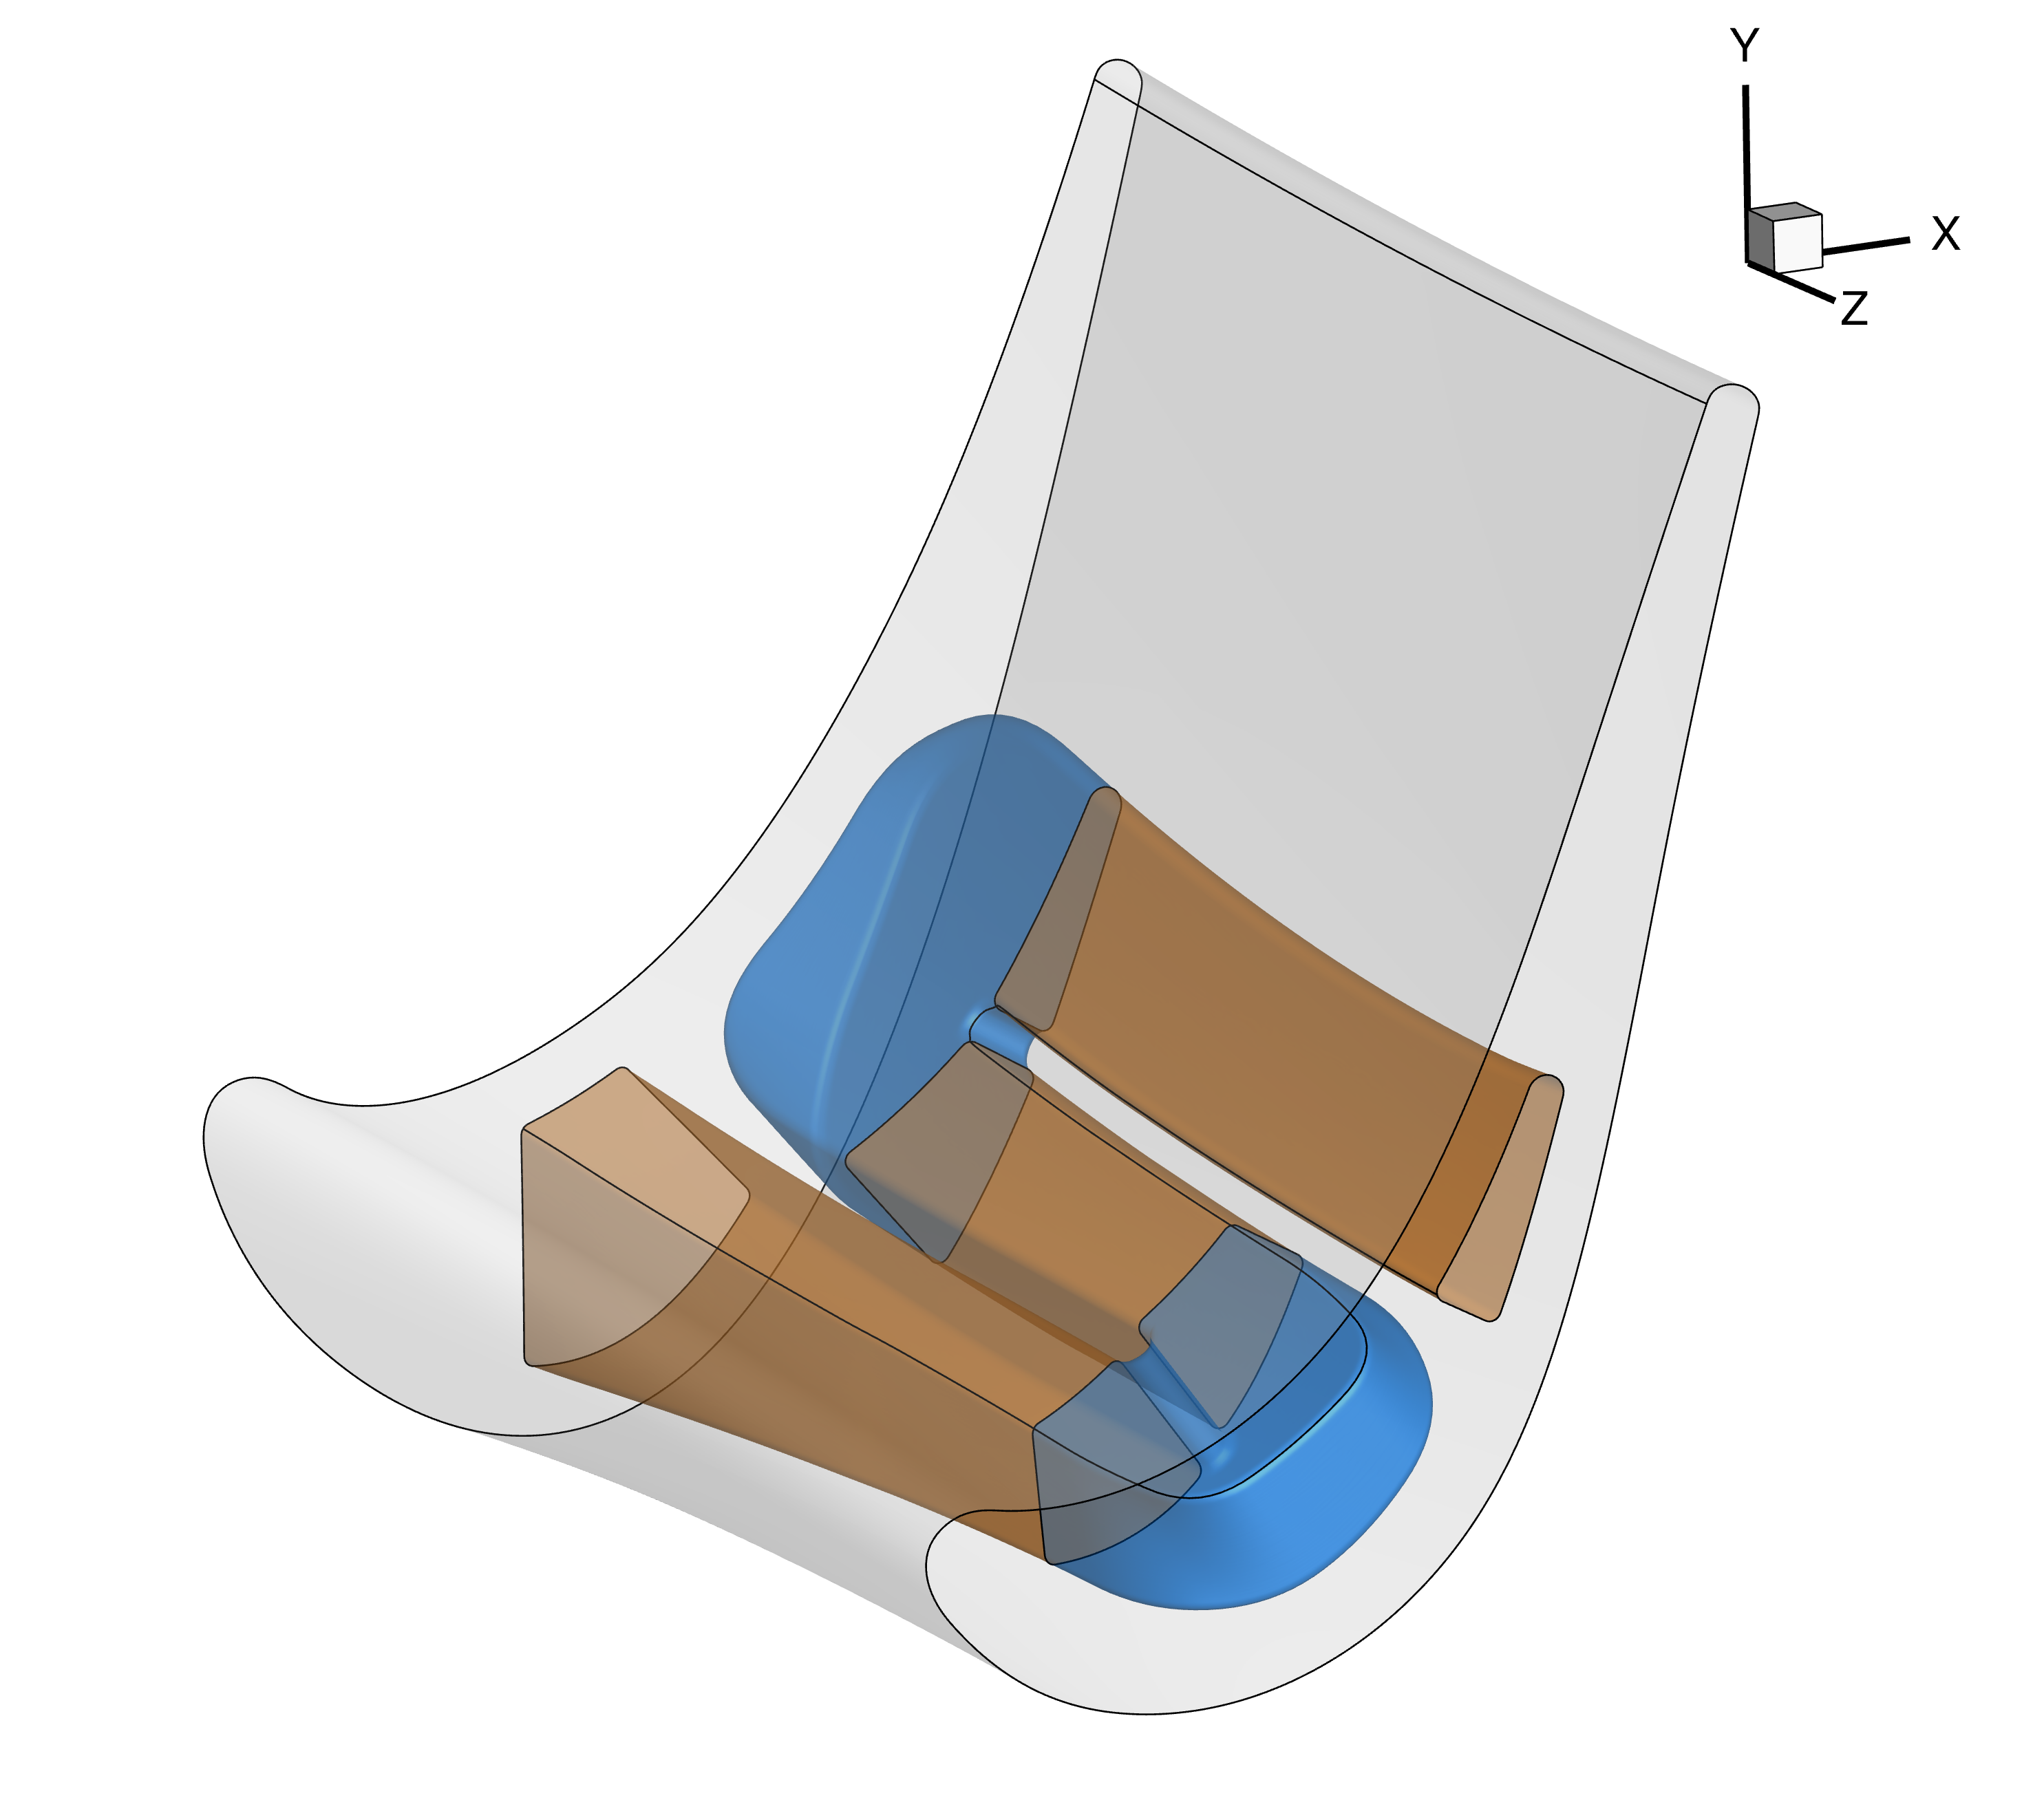
\includegraphics[width=\textwidth]{../tec/complete/020.png}
		\end{subfigure}
		\begin{subfigure}{.49\textwidth}
			\centering
			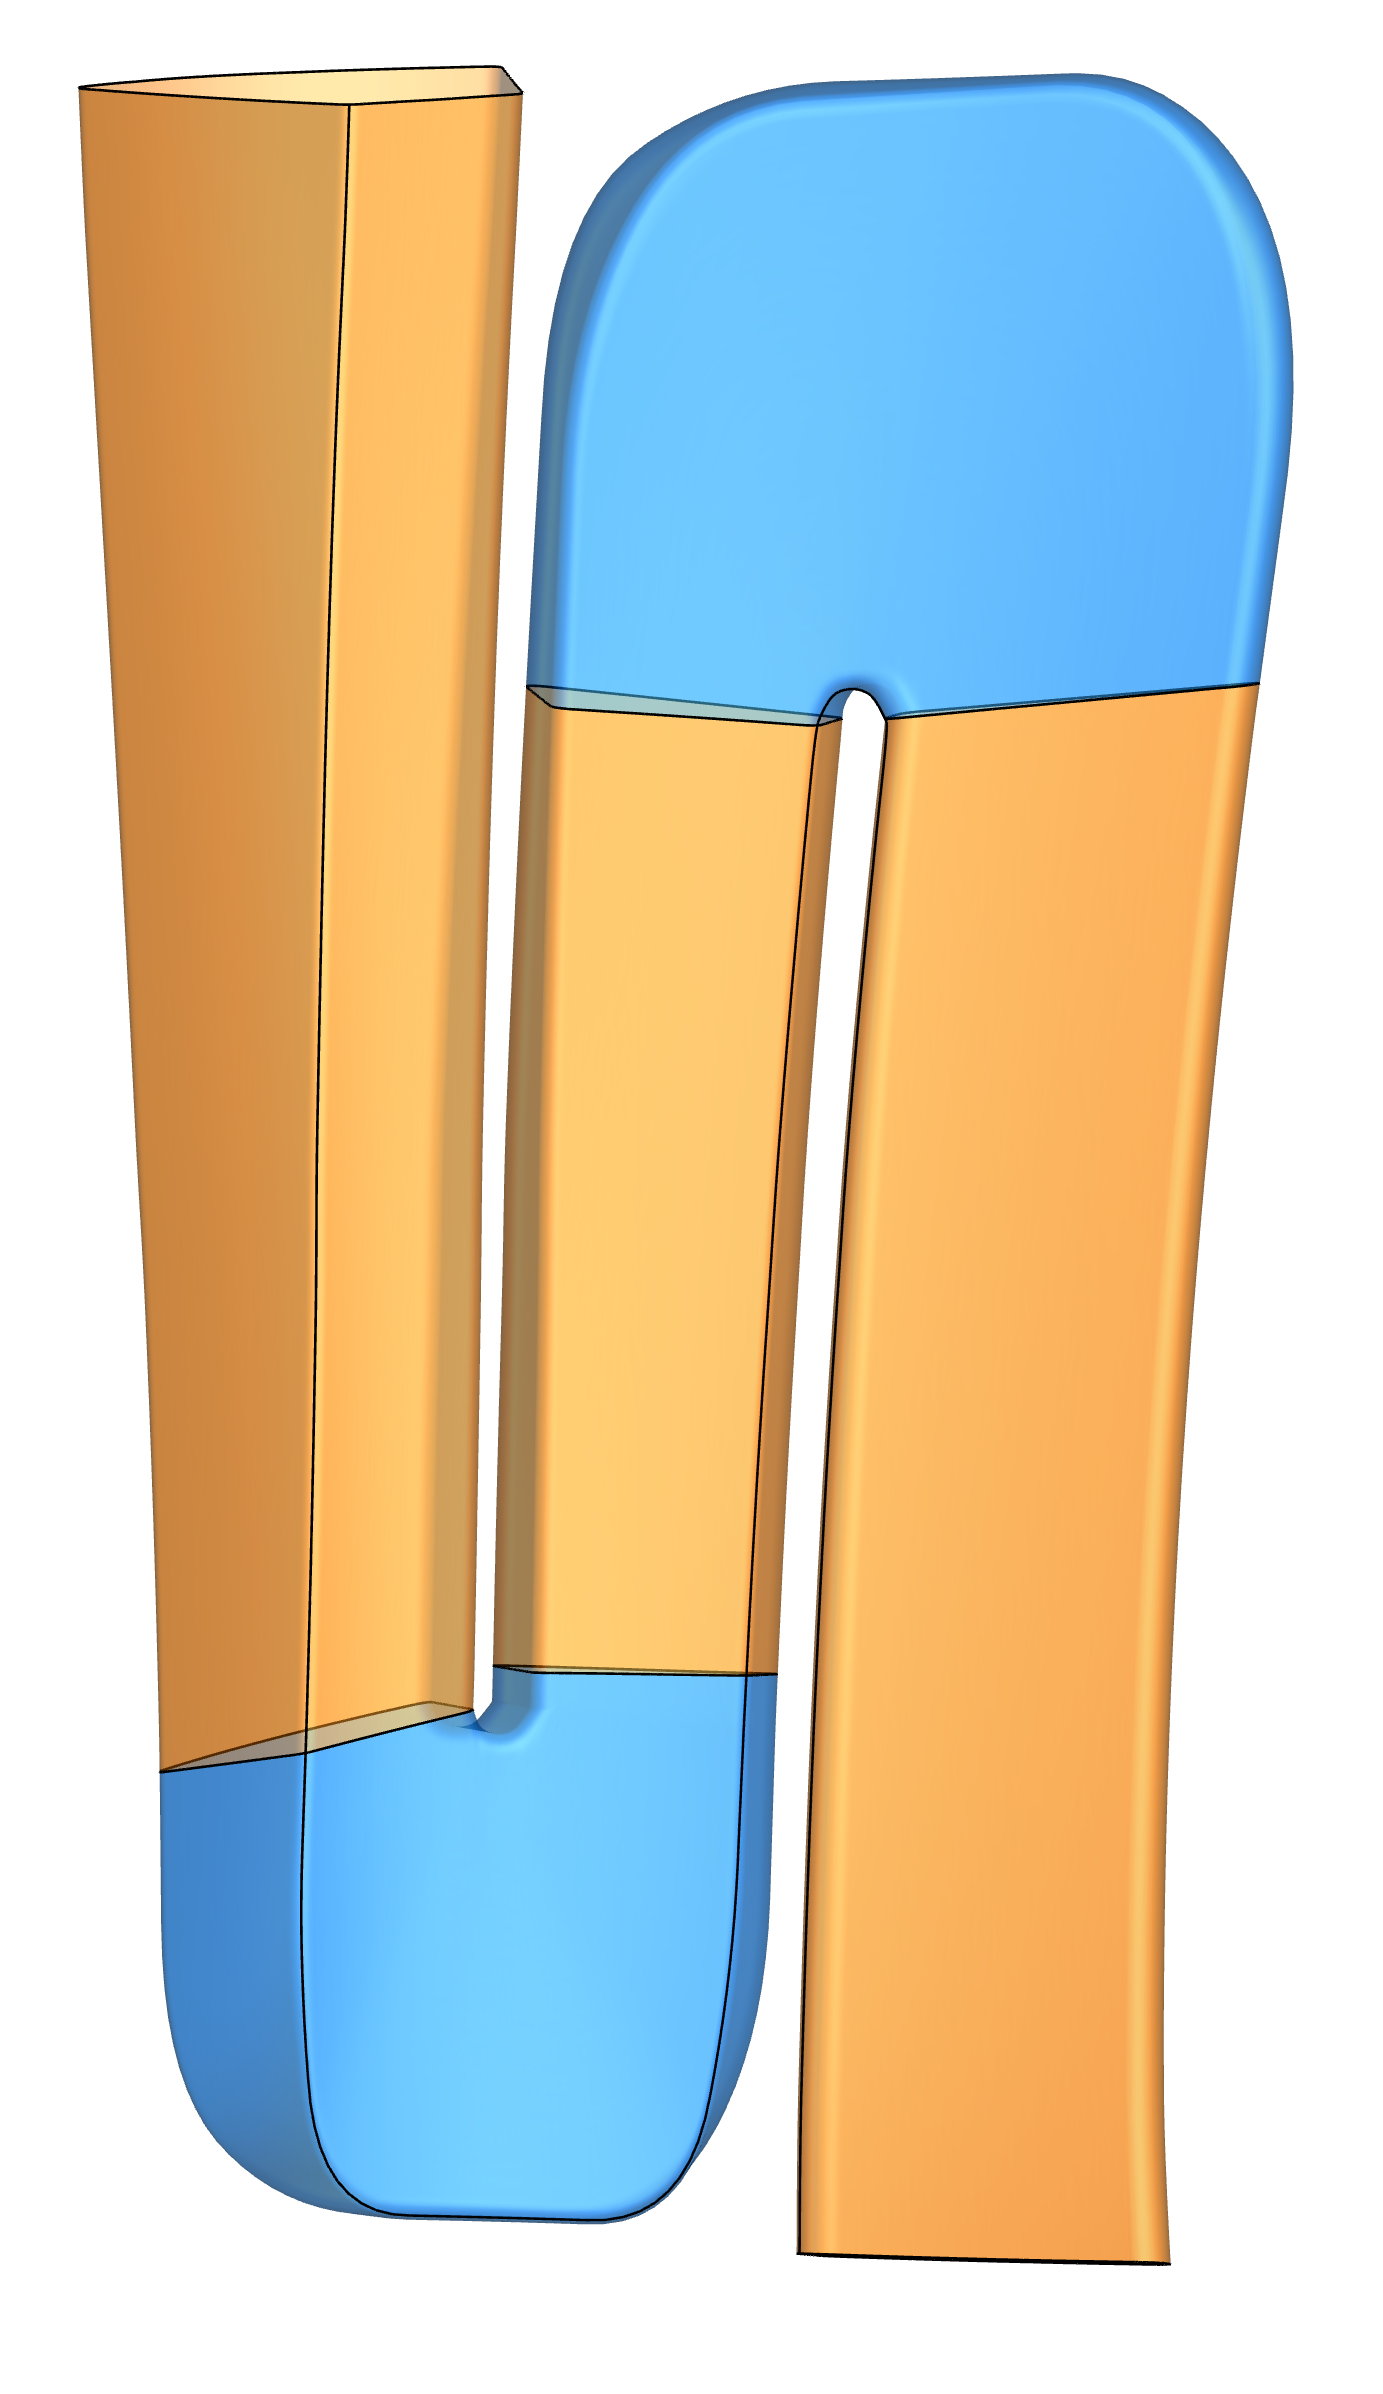
\includegraphics[width=.5\textwidth]{../tec/complete/021.png}
		\end{subfigure}
		\caption{Distinguishing chambers (orange) and turns (blue) in a channel.}
		\label{fig:chambers_vs_turns}
	\end{figure}

\subsection{Chambers}\label{sec:chambers}
	The construction of chambers of a cooling channel is presented in this section.

	\begin{figure}[H]
		\centering
		\begin{subfigure}{.32\textwidth}
			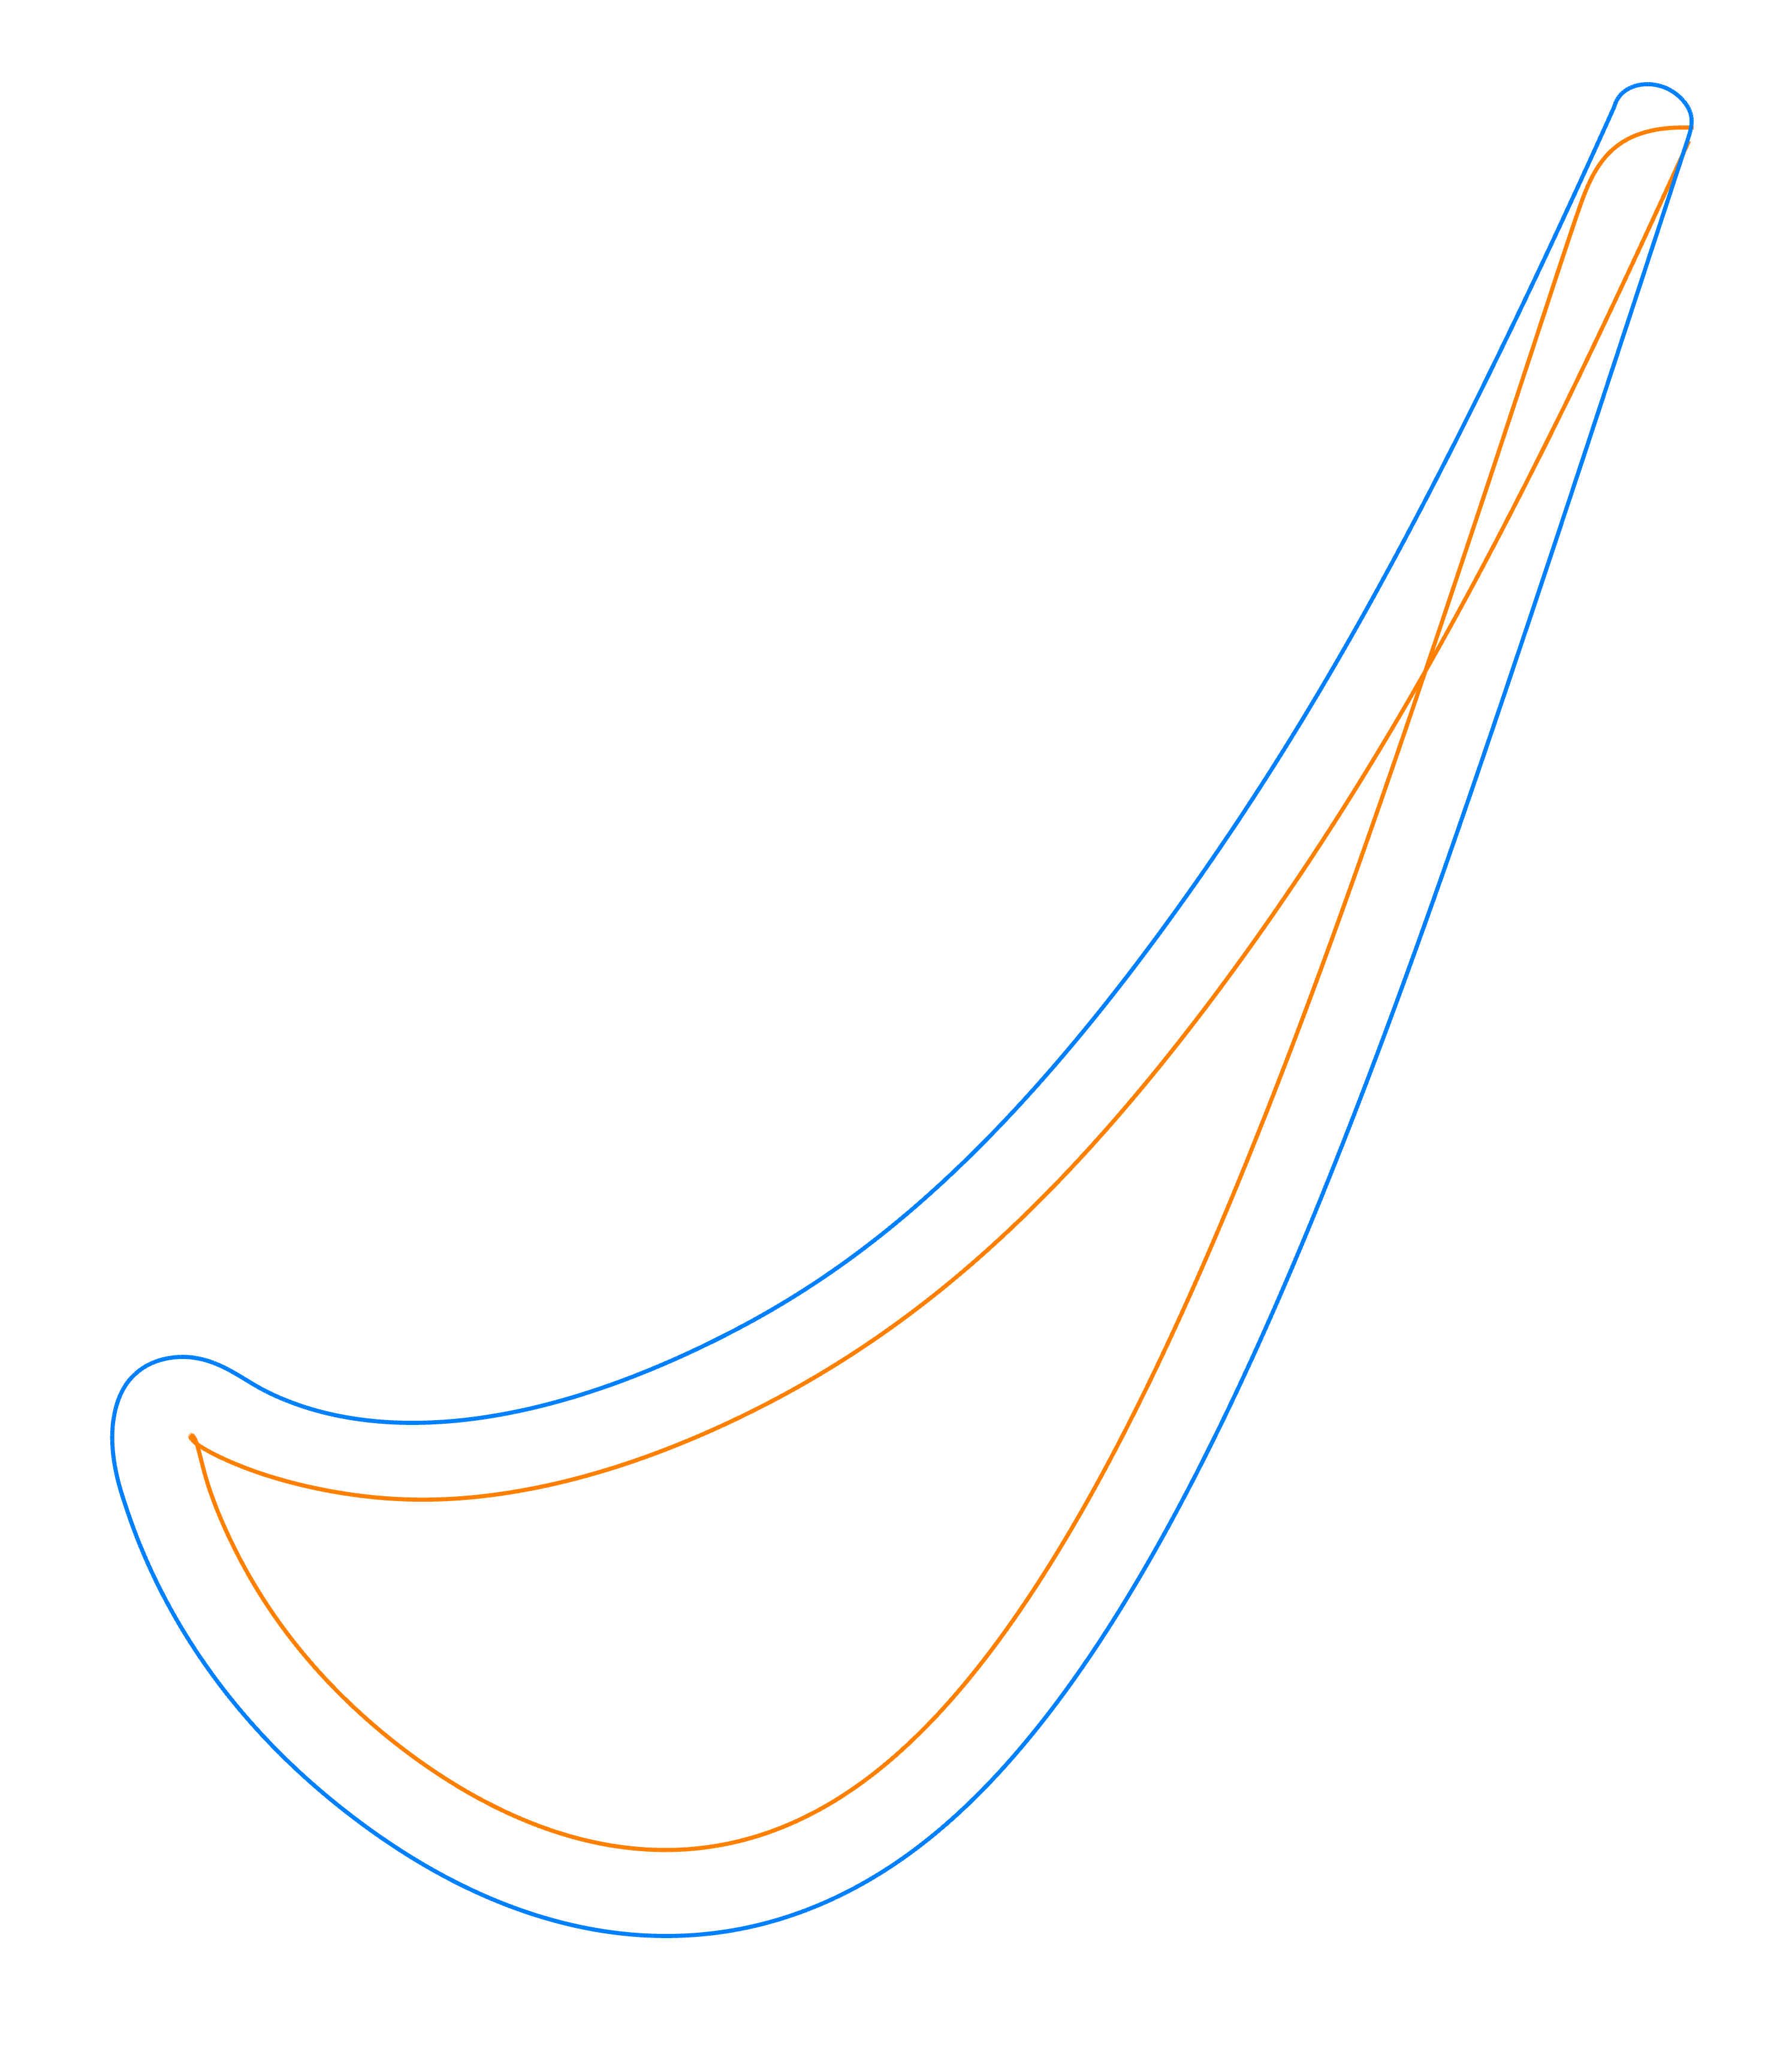
\includegraphics[width=\textwidth]{../tec/shrinking/61.png}
			\caption{Offsetting.}
		\end{subfigure}
		\begin{subfigure}{.32\textwidth}
			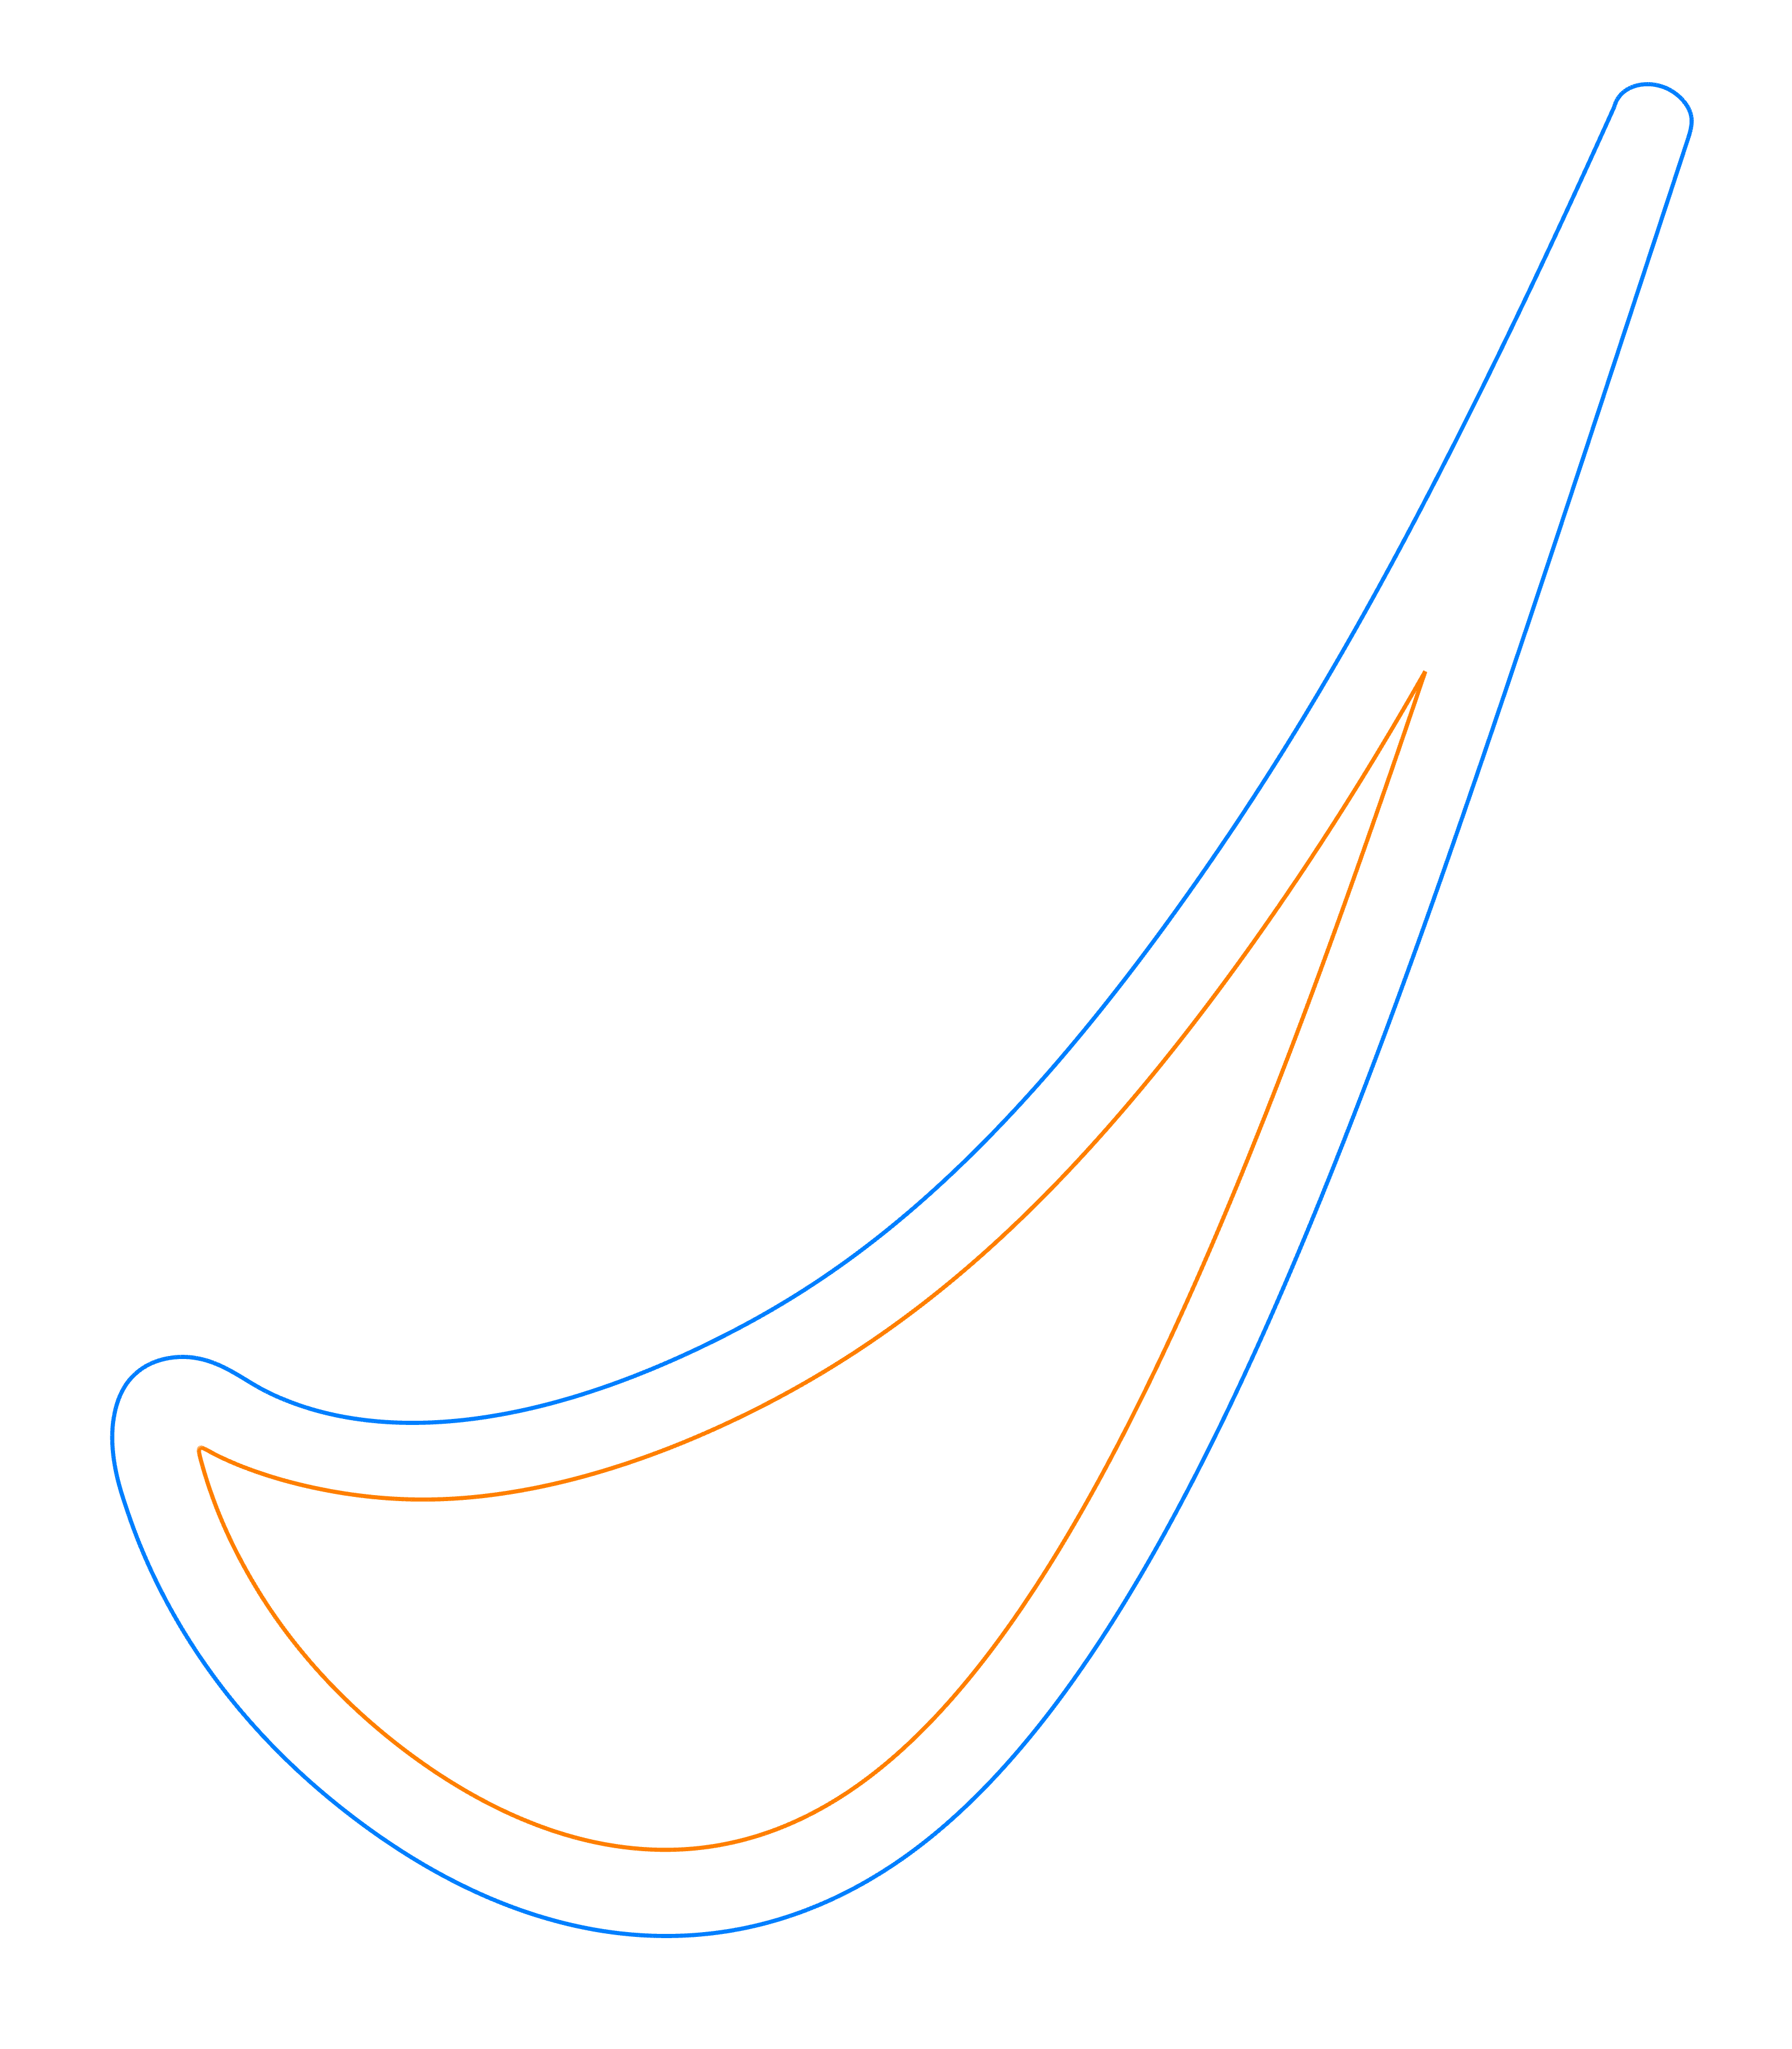
\includegraphics[width=\textwidth]{../tec/shrinking/62.png}
			\caption{Trimming.}
		\end{subfigure}
		\begin{subfigure}{.32\textwidth}
			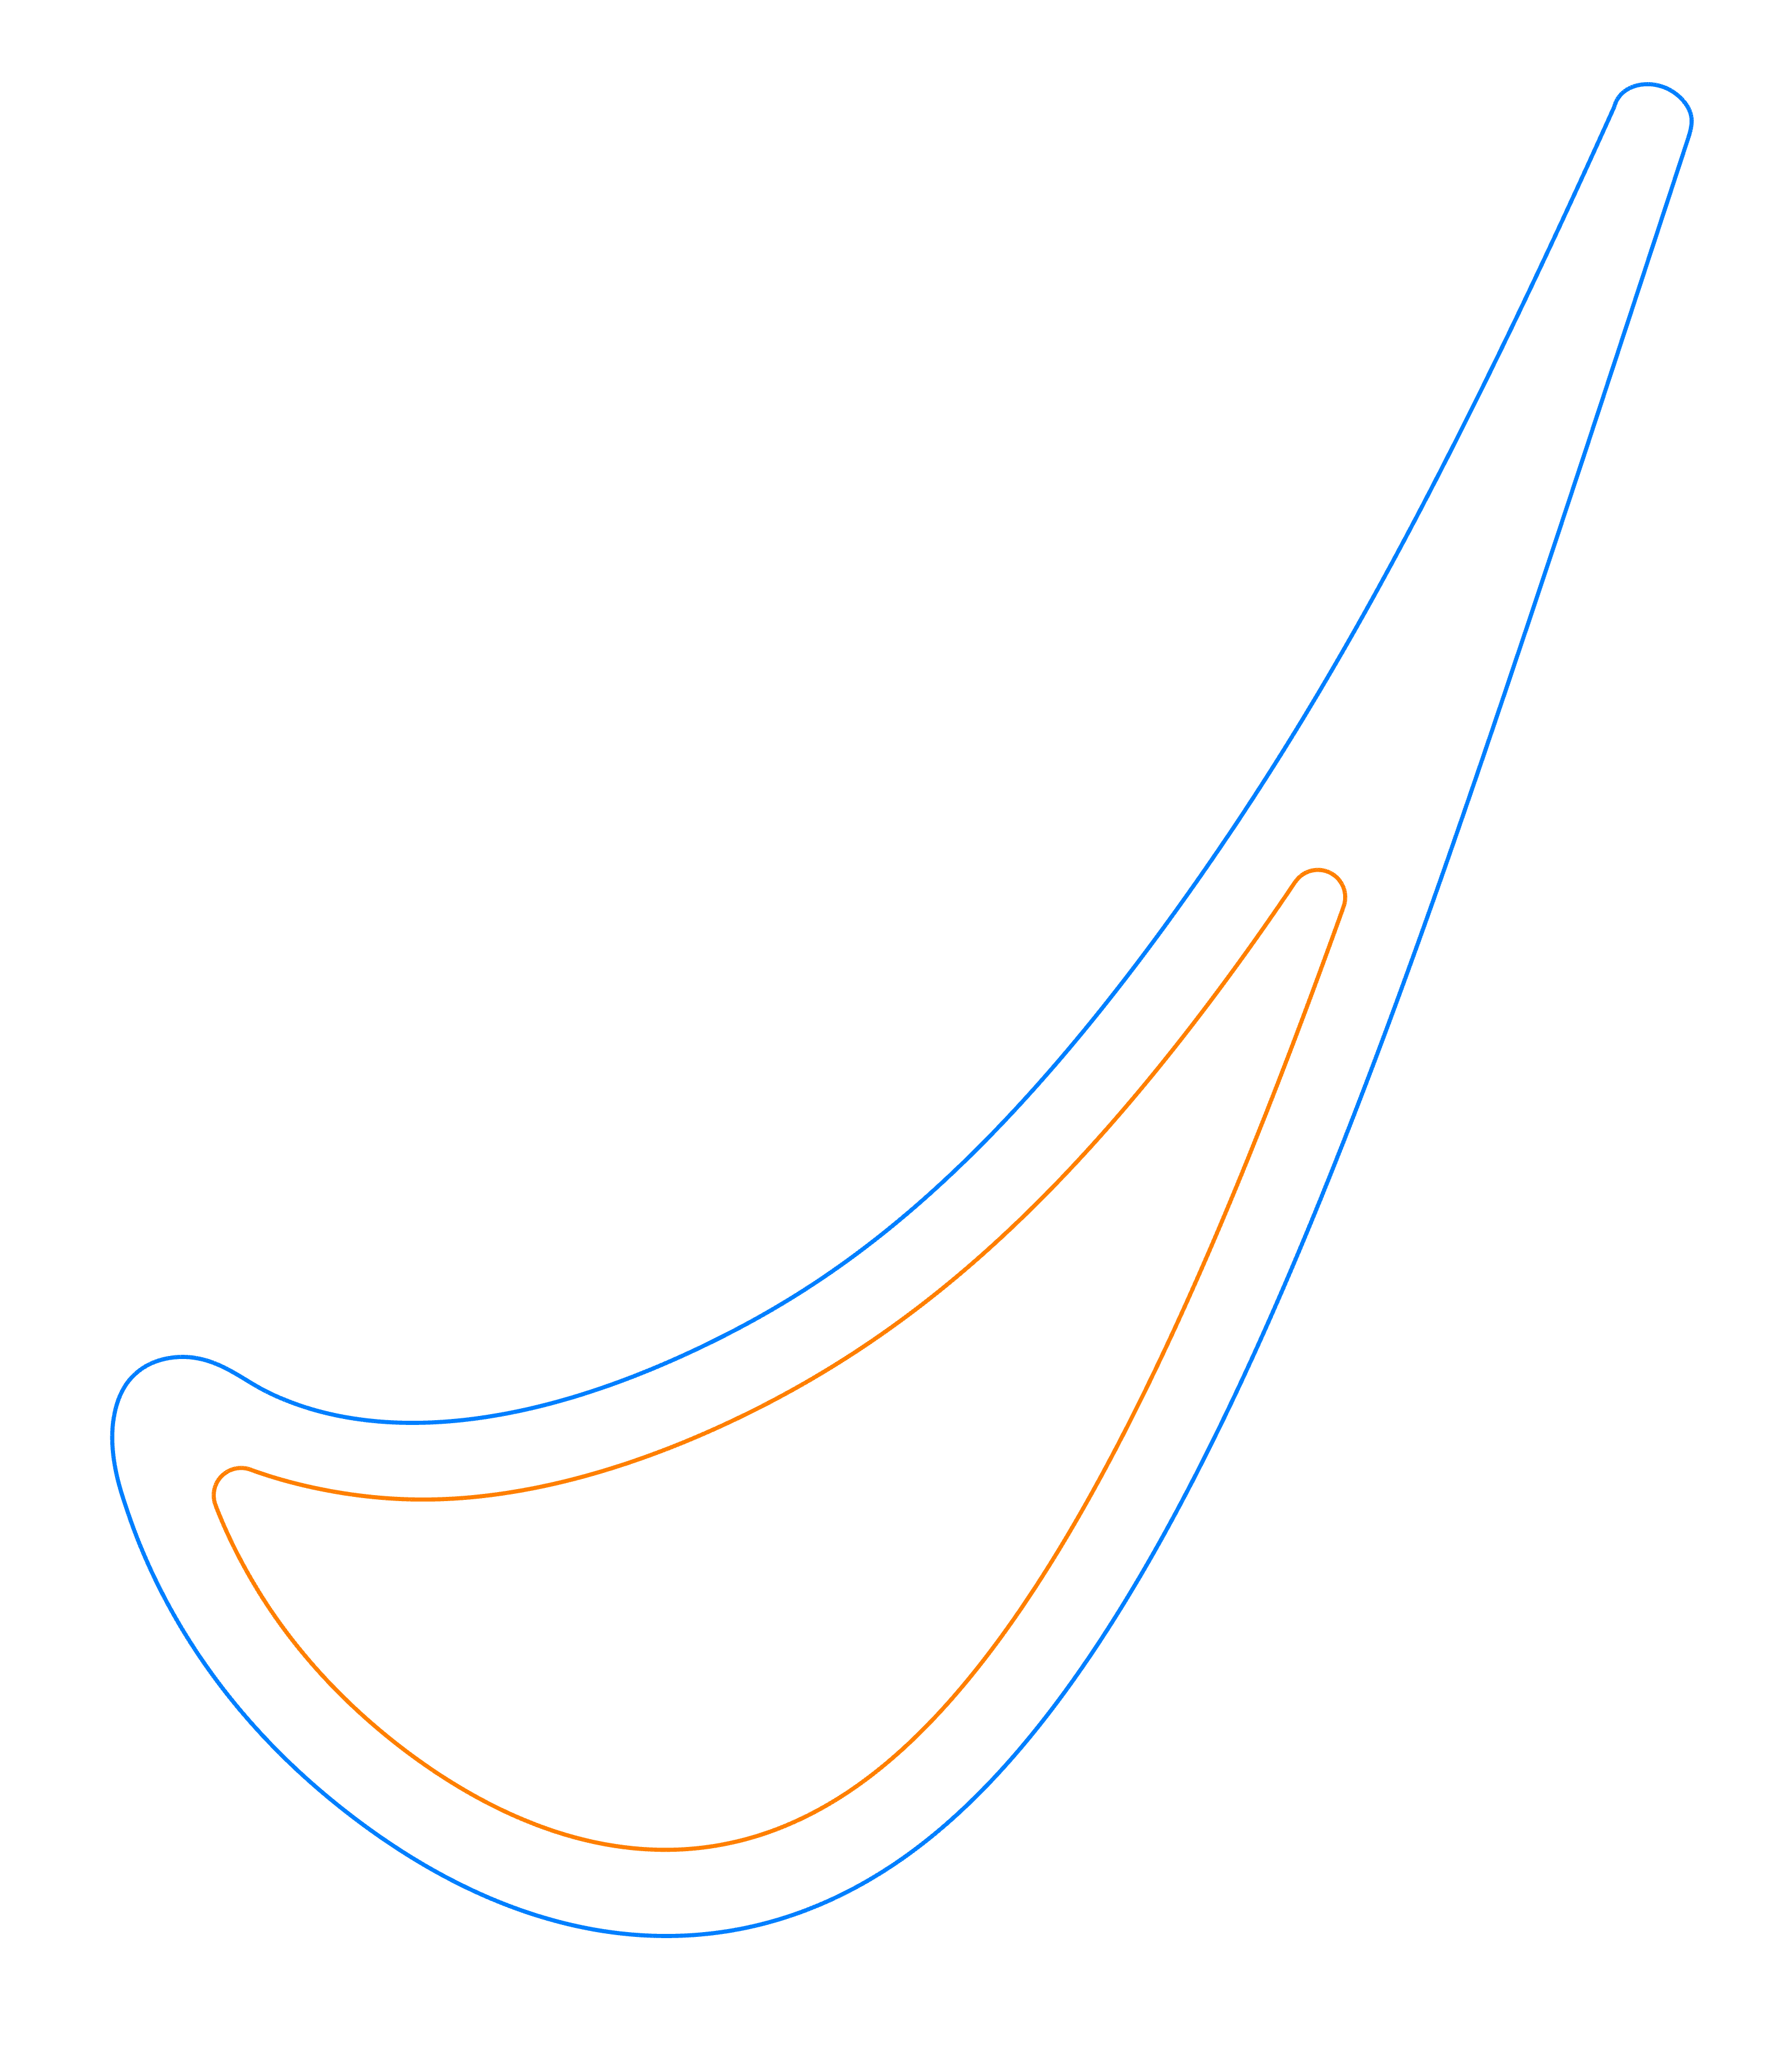
\includegraphics[width=\textwidth]{../tec/shrinking/63.png}
			\caption{Adding fillets.}
		\end{subfigure}
		\caption{Shrinking a profile in $(m, r\theta)$. The black curve represents $B^{(v_i)}_\textrm{stream}(u)$, whereas the red curve in (c) represents $S^{(v_i)}_\textrm{stream}(u)$.}
		\label{fig:profileshrinking}
	\end{figure}

	First, we apply the stream surface coordinate transformation presented in Section \ref{sec:mrtheta} to a fixed number $N$ of $v$-isoparametric curves of the blade (or vane) to calculate the profiles $B^{(v_i)}_\textrm{stream}(u)$ for $v_i \in [0,1]$, $i \in \{1,...,N\}$. These profiles are then offset by an input parameter. The profile is automatically trimmed adequately (as described in Section \ref{sec:offsetcurves}) and fillets are added to round off the emerging corners. The fillet radius is also declared as an input. We refer to the resulting profile as shrunk profile $S^{(v_i)}_\textrm{stream}(u)$. This process is depicted in Figure \ref{fig:profileshrinking}. The subdivision into leading edge, pressure side, suction side and trailing edge is kept by using the fillet boundaries as transition points.

	Next, we calculate the camber curve $c^{(v_i)}$ of each shrunk profile $S^{(v_i)}_\textrm{stream}$. The camber curve is a design aid which is defined by the following property. A point $x$ lies on the camber curve $c^{(v_i)}$ of $S^{(v_i)}_\textrm{stream}$ if and only if for some $d$ the offset curve $O^{S^{(v_i)}_\textrm{stream}}_d$ has a self intersection at $x$. Along the camber curve, we define the wall input, which is given by a set of parameters $w_j \in [0,1]$ representing the positions of each wall as parameter of the camber curve, $j \in \{1,...,N_C-1\}$, where $N_C$ is the number of chambers that shall be created. For each position, we also define an angle $\omega_j \in (0, \pi)$.

	\begin{figure}[H]
		\centering
		\begin{subfigure}{.65\textwidth}
			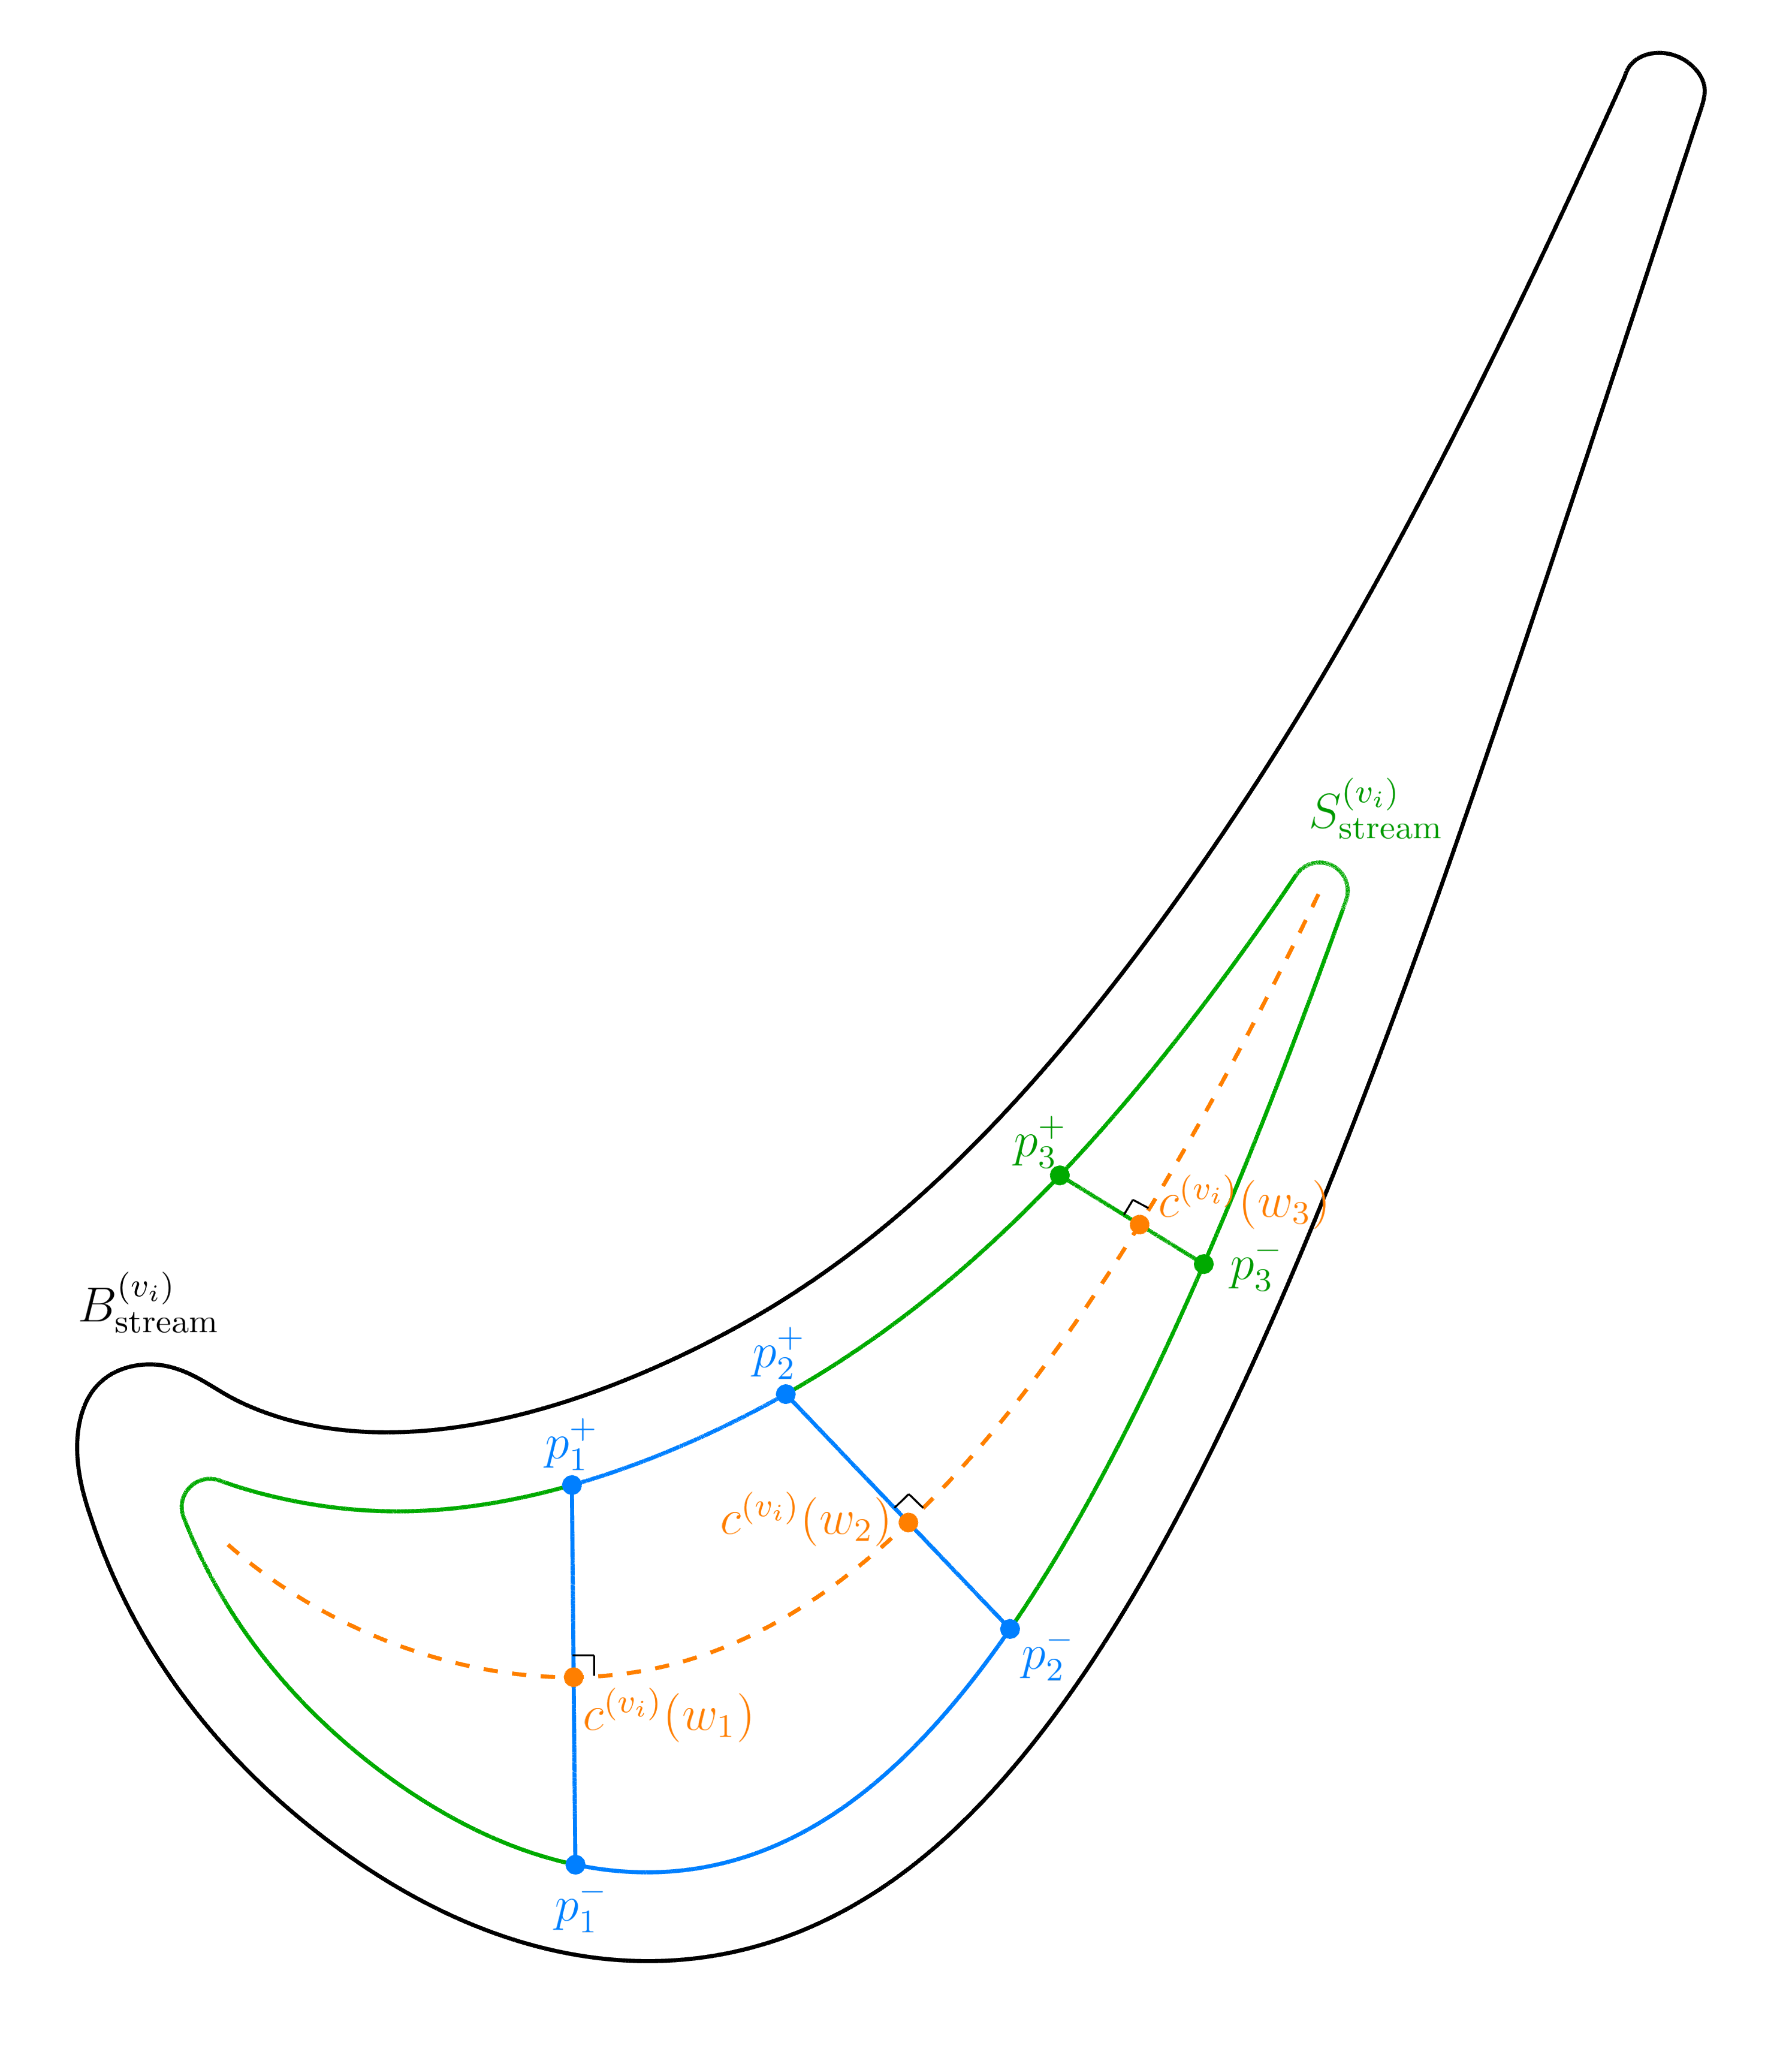
\includegraphics[width=\textwidth]{../tec/chambers/61.png}
			\caption{Partitioning the profile.}
		\end{subfigure}
		\begin{subfigure}{.33\textwidth}
			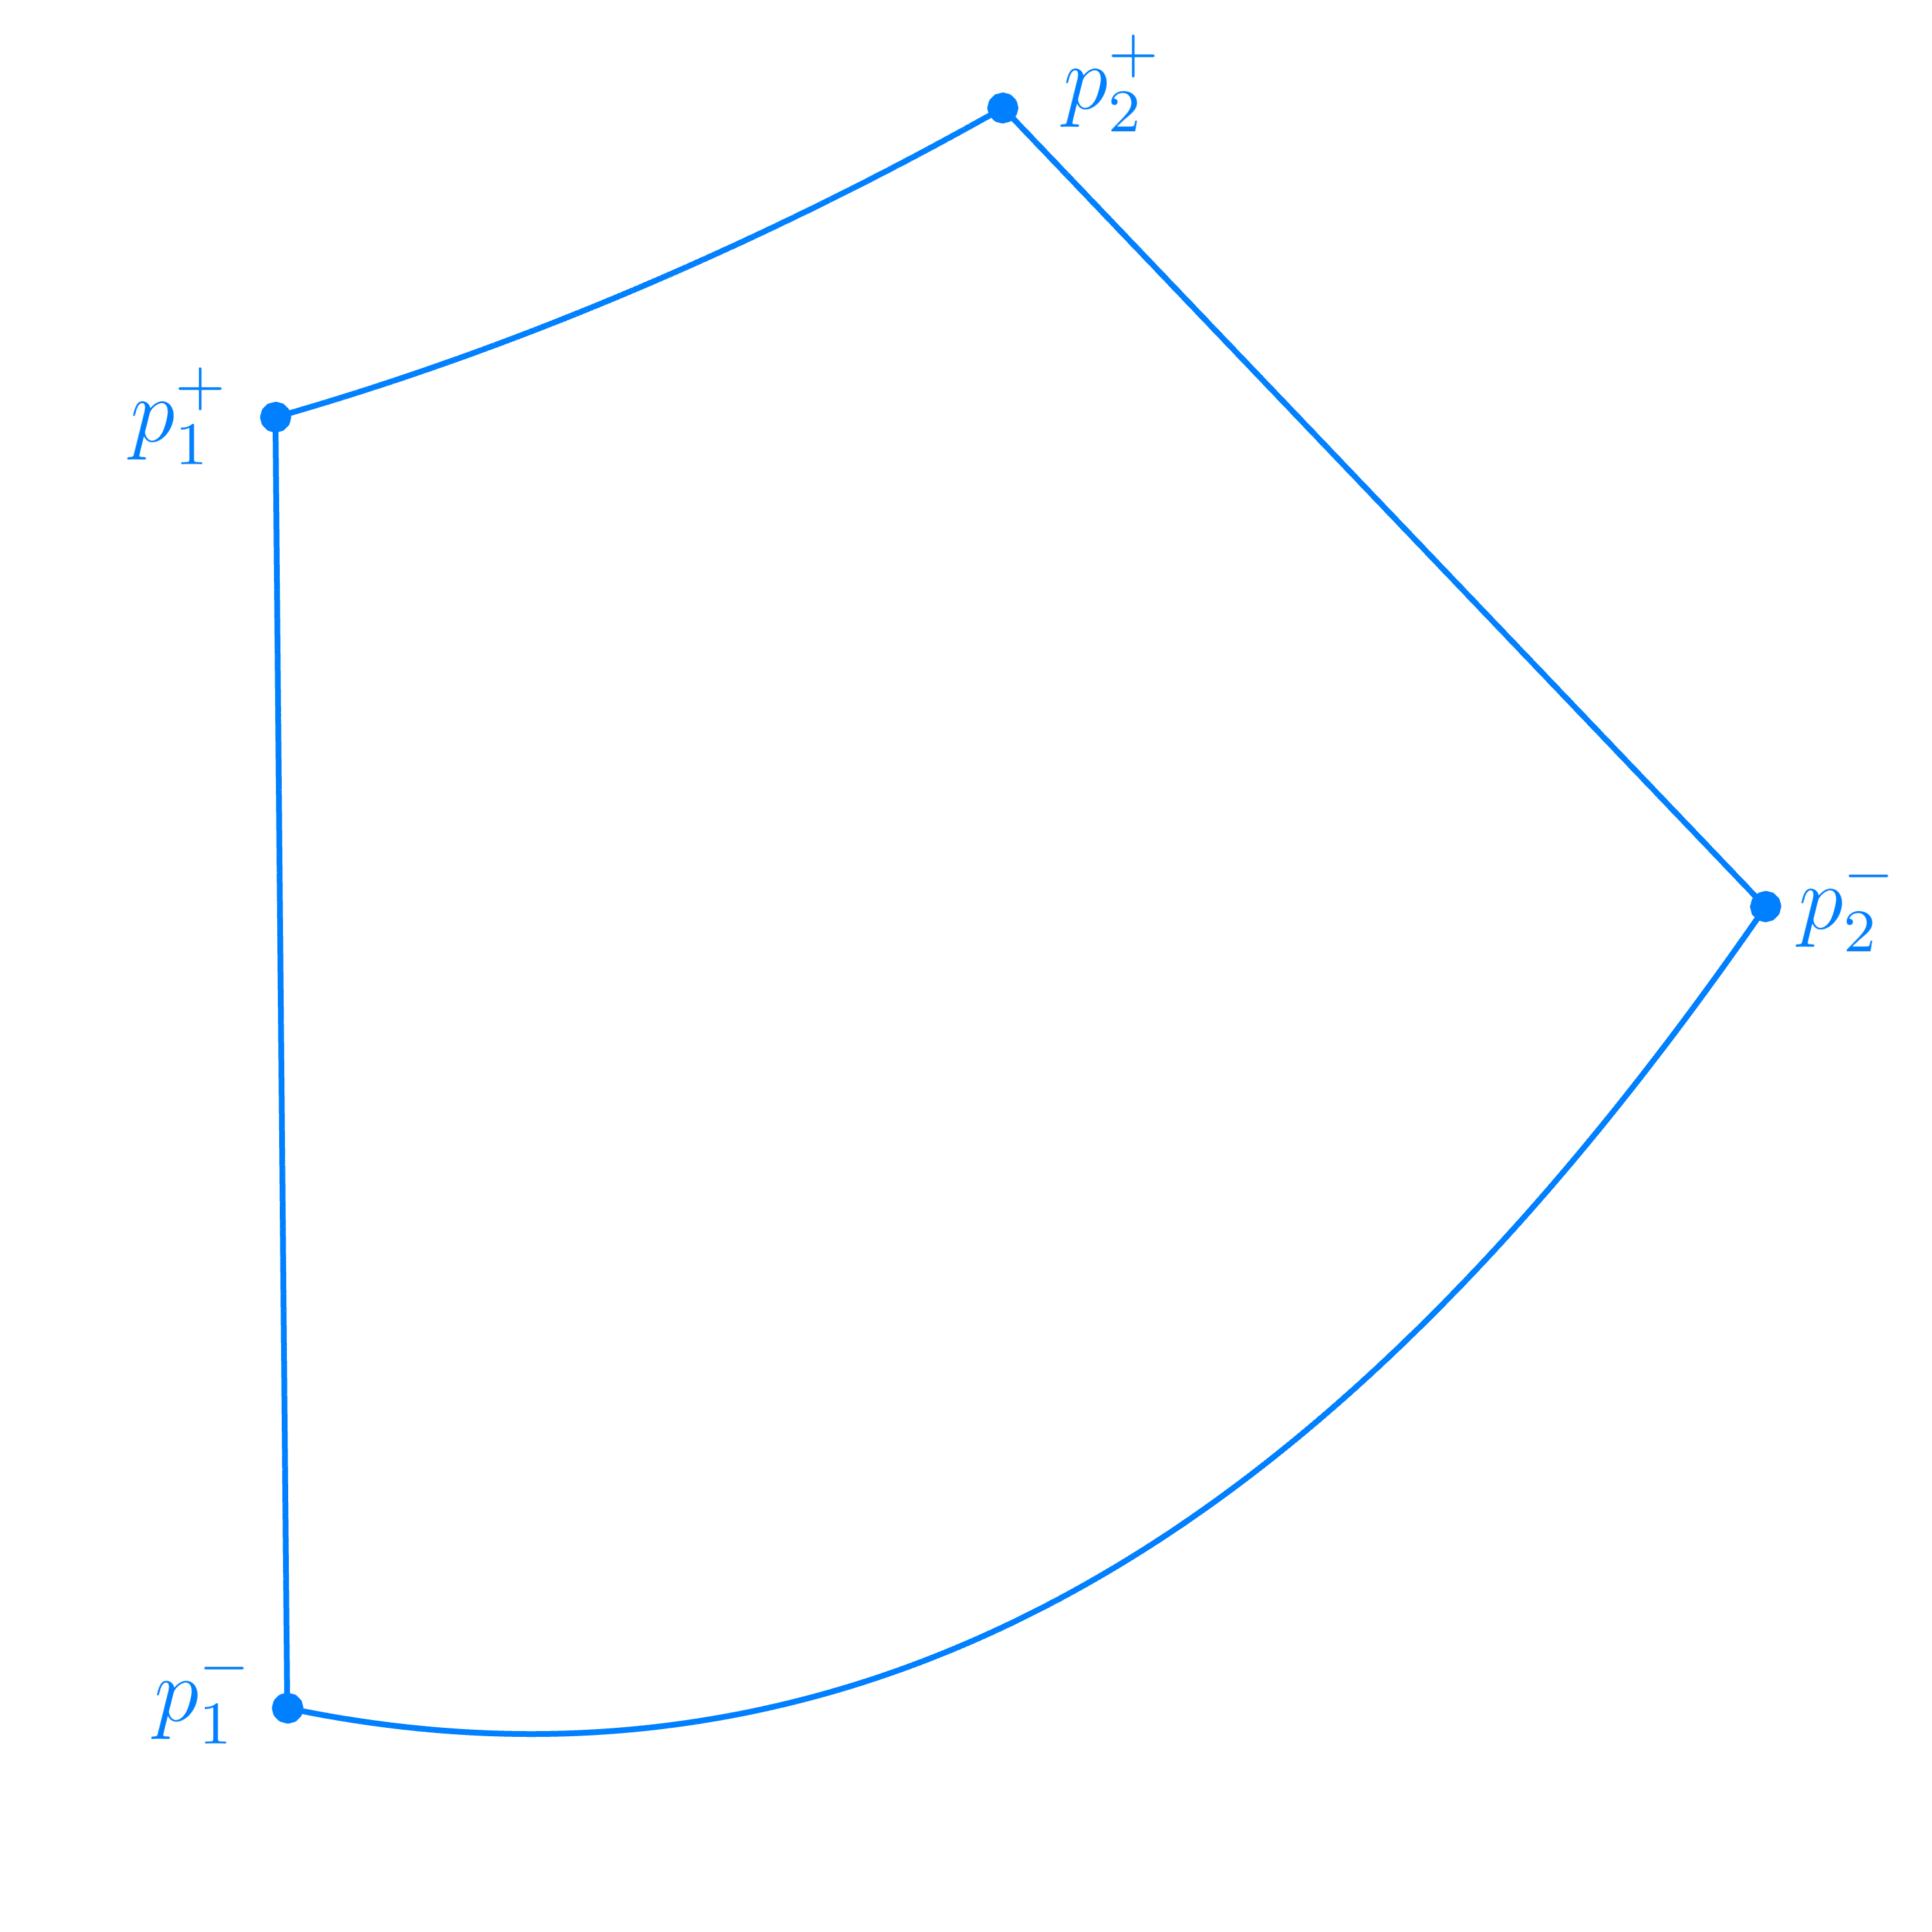
\includegraphics[width=\textwidth]{../tec/chambers/62.png}
			\vspace{2cm}
			\caption{Resulting partition.}
		\end{subfigure}
		\caption{Profile partitioning along rays that emerge from the camber curve. The camber curve is represented by the dashed line. In this example, we create three chambers. The walls are represented by the line segments $\overline{p_1^+p_1^-}$ and $\overline{p_2^+p_2^-}$.}
		\label{fig:subdivision_chamber}
	\end{figure}

	Each position-angle pair represents two rays
		$$ c(w_j) + sR_{\omega_j} \nabla c(w_j) \quad\text{and}\quad c(w_j) - sR_{\omega_j} \nabla c(w_j) $$
	for $s \in [0, \infty)$, where $R_{\omega_j}$ is a rotation matrix like presented in Equation (\ref{eq:rotationmat}). Using Algorithm \ref{alg:raymarching}, we can find the respective intersection points $p_j^+$ and $p_j^-$ of the rays and the shrunk profile $S^{(v_i)}_\textrm{stream}$. The line segment $\overline{p_j^+p_j^-}$ now represents the $j$-th wall. This process is repeated for all $j \in \{1,...,N_C-1\}$.

	Next, the blade (or vane) is partitioned at the intersection points $p_j^+$ and $p_j^-$ for all $j \in \{1,...,N_C-1\}$. For each such partitioning, we are left with four chamber-delimiting curves per chamber profile. This procedure is exemplified in Figure \ref{fig:subdivision_chamber}. If there is only one chamber, the a priori partitioning scheme (leading edge, suction side, pressure side and trailing edge) is kept. In case of multiple chambers, the leading and trailing chambers have to be treated differently, because in this case each of them are delimited by only one wall. In this case, we use the leading edge partition or trailing edge partition in place of a wall.

	\begin{figure}[H]
		\begin{subfigure}{.32\textwidth}
			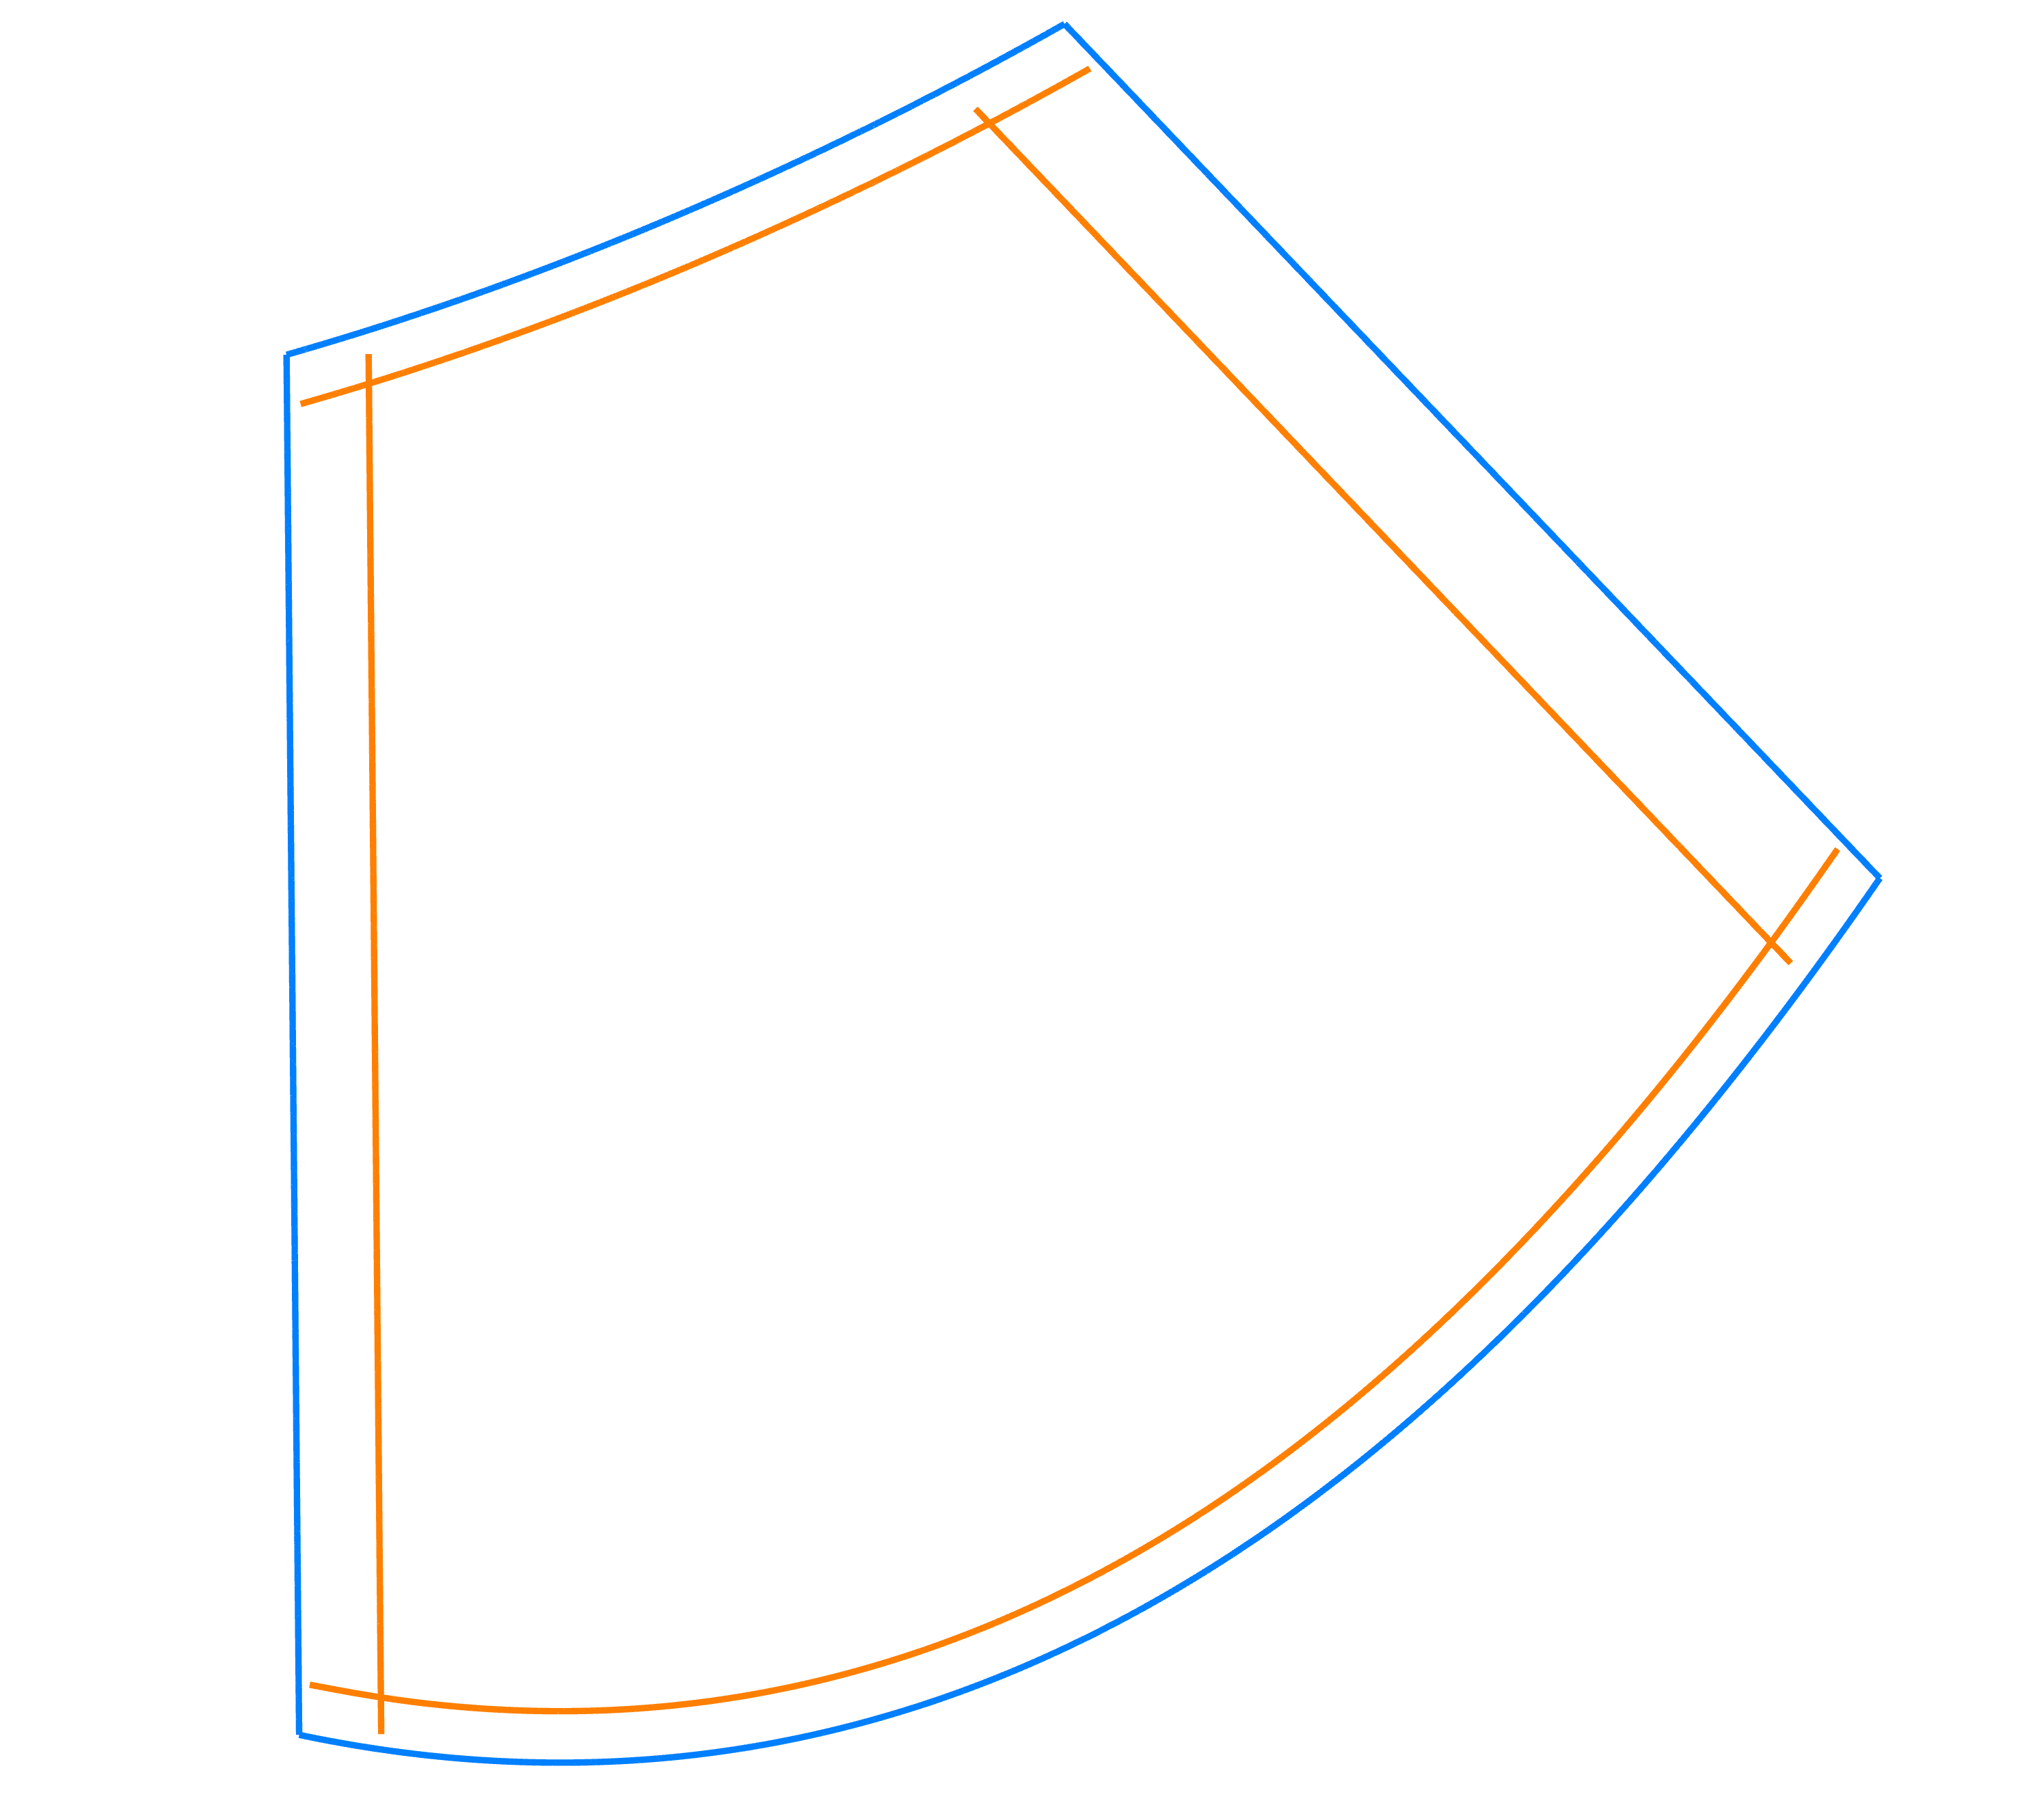
\includegraphics[width=\textwidth]{../tec/chambers/81.png}
			\caption{Offsetting.}
		\end{subfigure}
		\begin{subfigure}{.32\textwidth}
			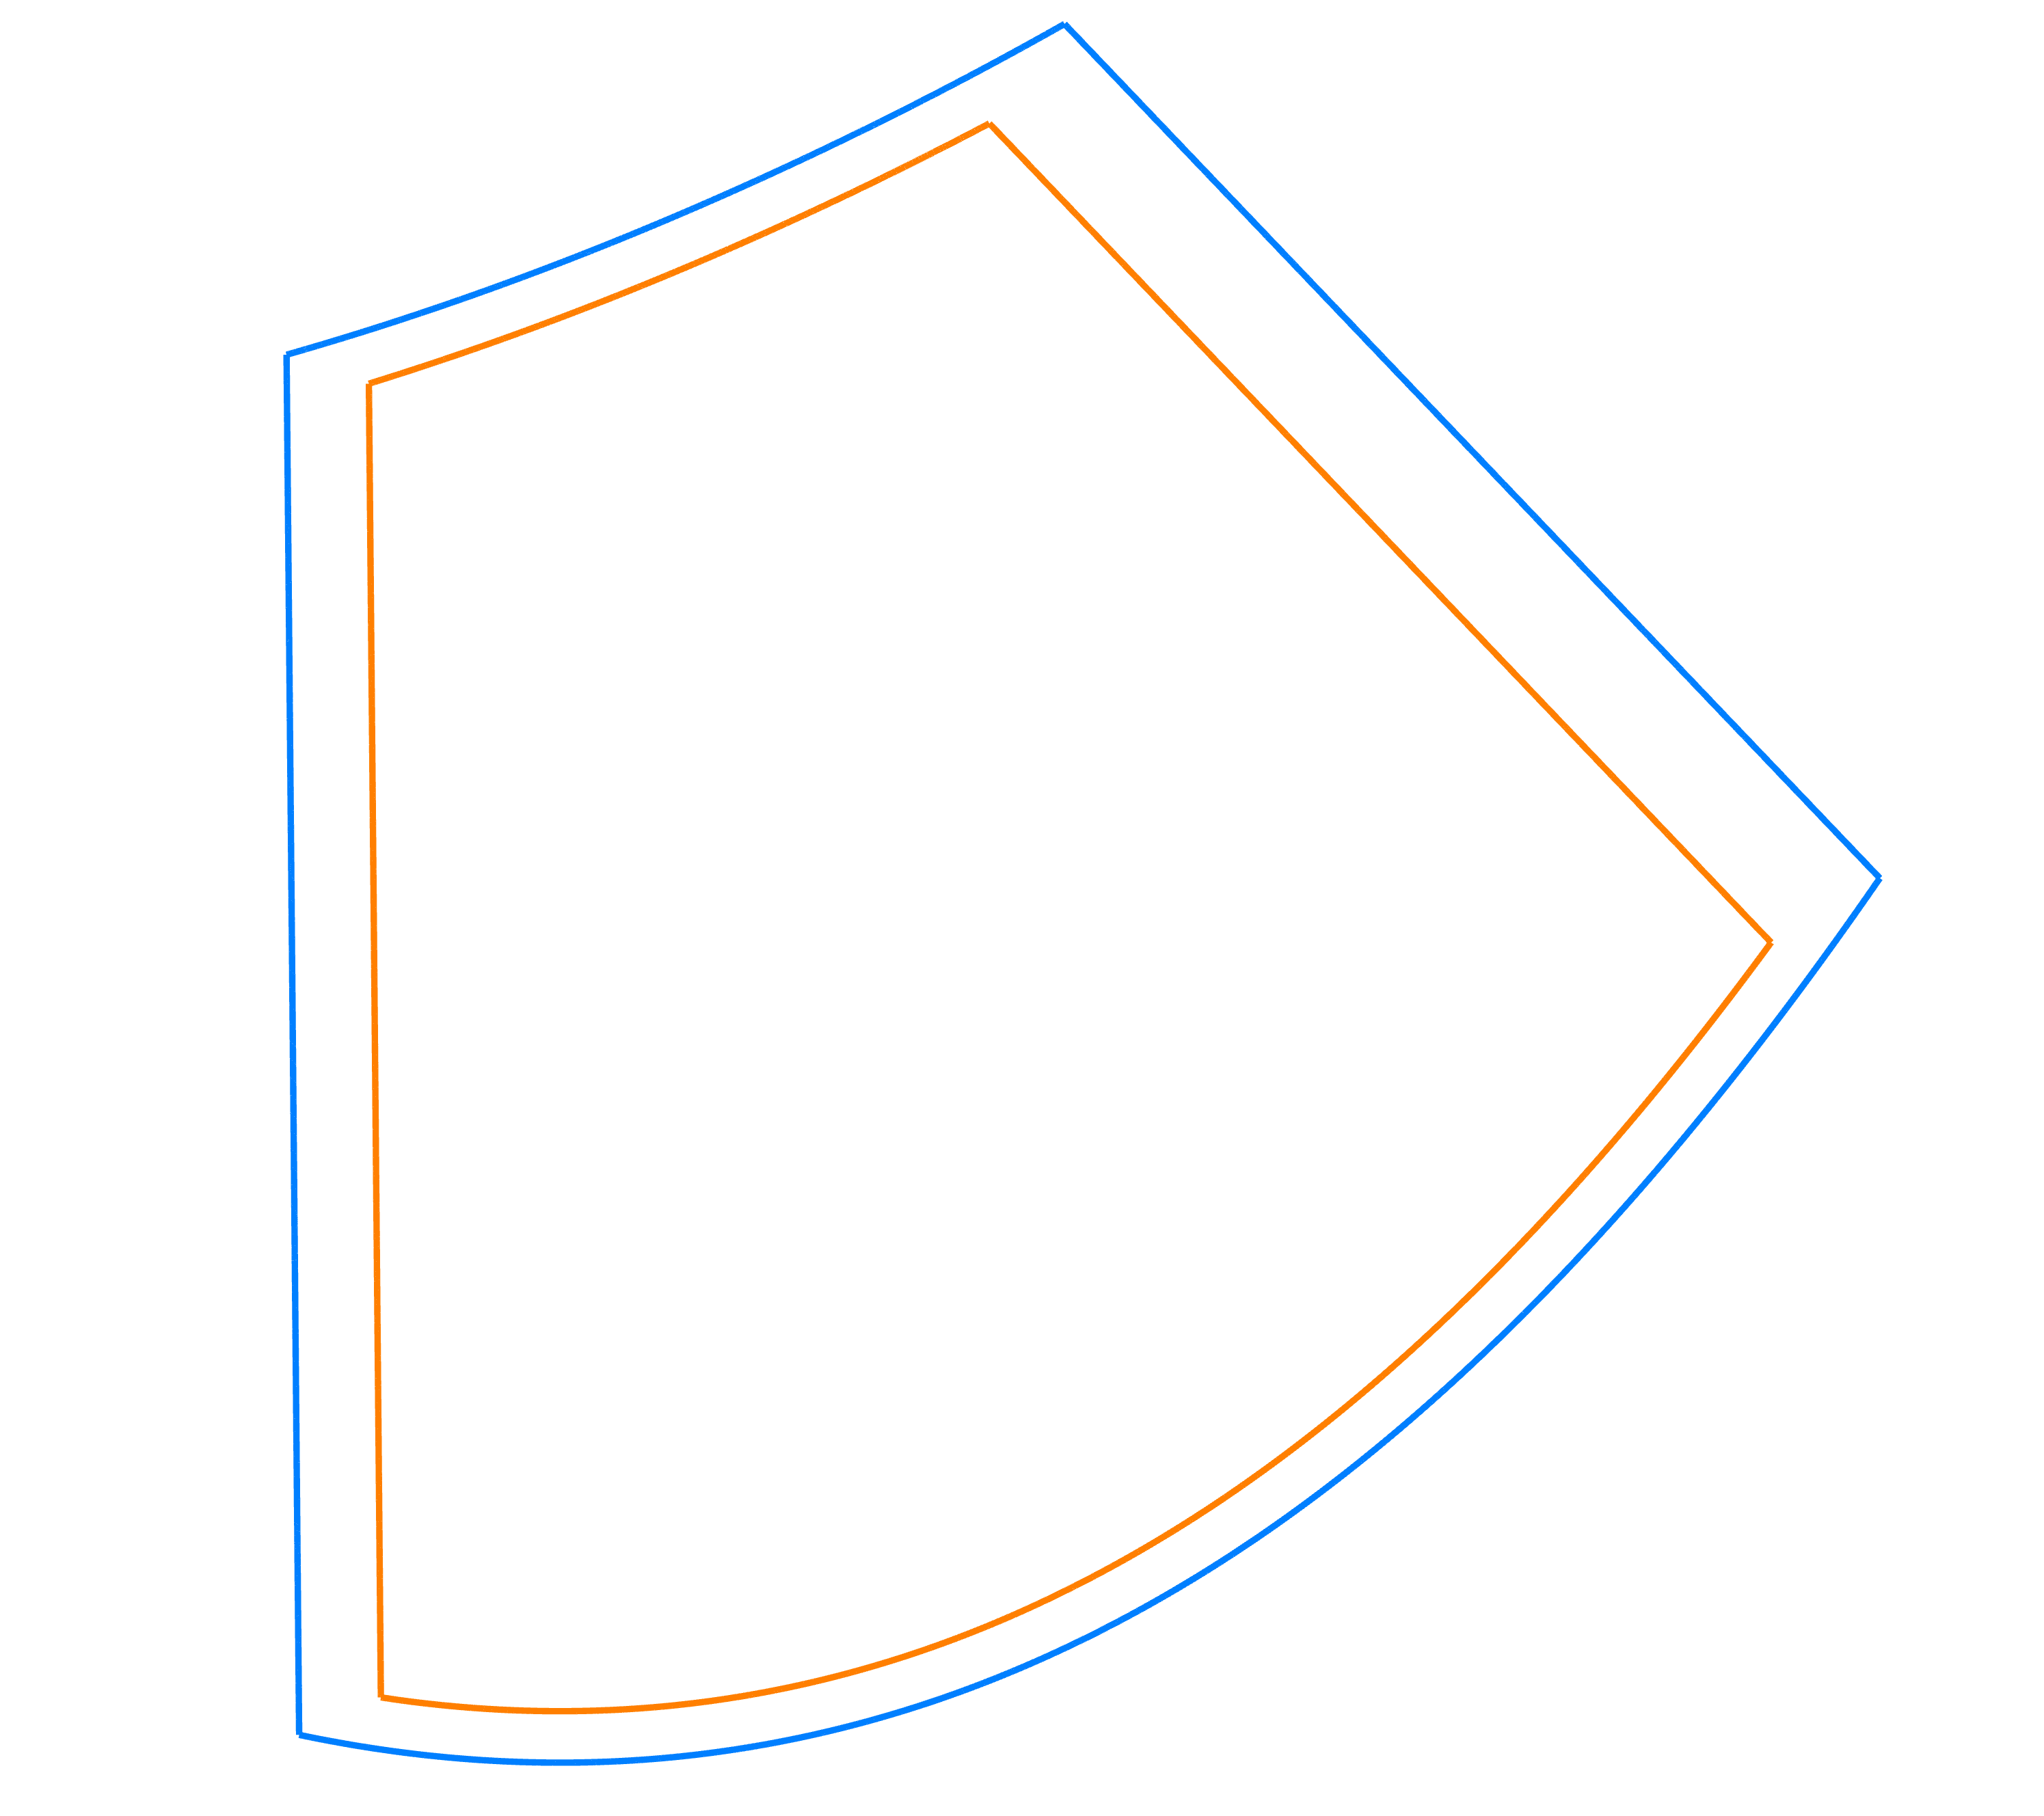
\includegraphics[width=\textwidth]{../tec/chambers/82.png}
			\caption{Trimming.}
		\end{subfigure}
		\begin{subfigure}{.32\textwidth}
			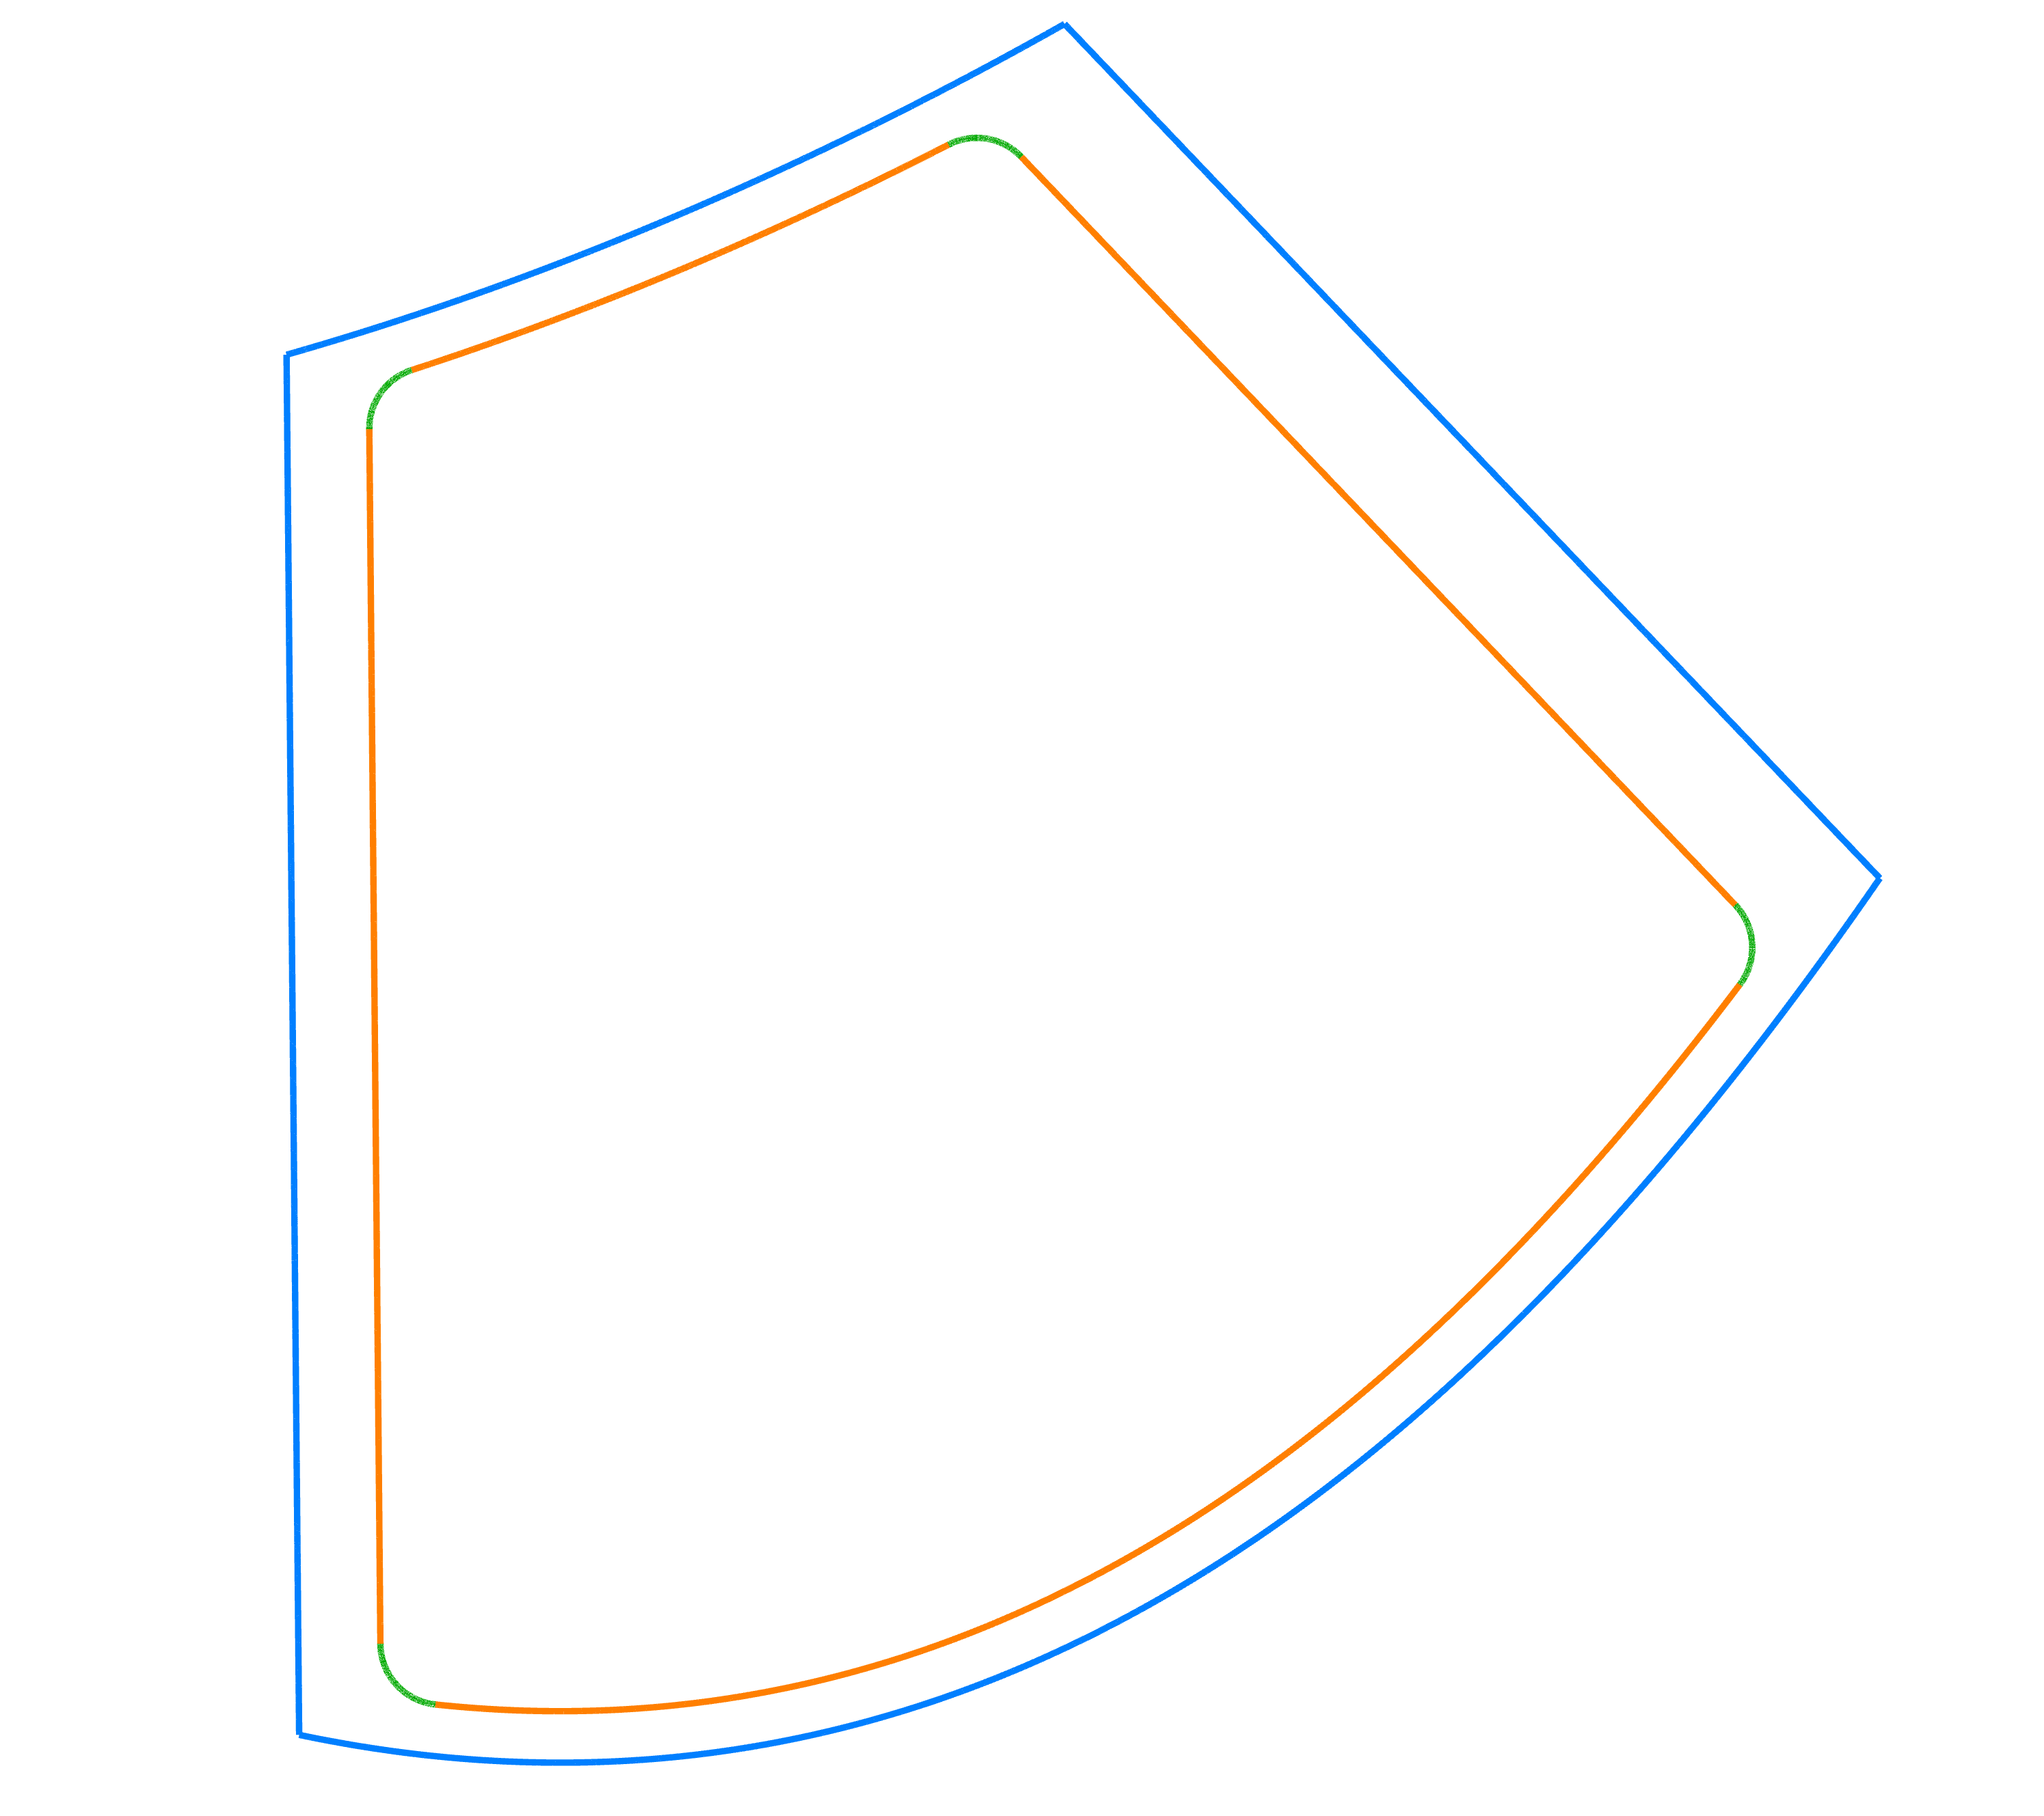
\includegraphics[width=\textwidth]{../tec/chambers/83.png}
			\caption{Adding fillets.}
		\end{subfigure}
		\caption{Construction of a chamber profile.}
		\label{fig:chamber_shrinking}
	\end{figure}

	After partitioning, we offset the chamber-delimiting curves. Each chamber-delimiting curve is offset differently. In the wall input, the thickness of the wall in each direction is specified as an input. In fact, this input specification is done using two B-spline curves. For each wall, the user of CoolingGen specifies two sets control points $\{(v^1_k, d^1_k) : k \in \{1, ..., K\}\}$ and $\{(v^2_j, d^2_j) : j \in \{1, ..., J\}\}$, where $v^1_k, v^2_j \in [0,1]$ are surface parameters and $d^1_k$ are the respective thicknesses of the leading and trailing walls, respectively. Similarly, the suction and pressure side thicknesses for each chamber are defined by two B-spline curves.

	\begin{figure}[H]
		\centering
		\begin{subfigure}{0.28\textwidth}
			\centering
			\includesvg[width=\textwidth]{../python/linearContinuationCurve}
			\caption{Linear continuation.}
		\end{subfigure}
		\begin{subfigure}{0.28\textwidth}
			\centering
			\includesvg[width=\textwidth]{../python/linearContinuationCurve2}
			\caption{Intersection of (a).}
		\end{subfigure}
		\begin{subfigure}{0.42\textwidth}
			\centering
			\includesvg[width=\textwidth]{../python/linearInterpolationOffset}
			\caption{Linear interpolation offset curve.}
		\end{subfigure}
		\caption{Ensuring curve connections. Figures (a) and (b) show the intersection of the linear continuation of two curves. Figure (c) shows a typical trailing edge arrangement of a pressure side profile $\gamma_1$ (blue) offset by $d_1$ and a suction side profile $\gamma_2$ (green) offset by $d_2$. The trailing edge curve is offset at every point by a different value. We can write the linear interpolation offset curve of the trailing edge $\gamma_T$ as $O_{d_1, d_2}^{\gamma_T}(t) = (1-t)\,O_{d_1}^{\gamma_1} + t\,O_{d_2}^{\gamma_2} = O^{\gamma_T}_{(1-t)d_1 + td_2}(t)$ for all $t \in [0,1]$.}
		\label{fig:linear_continuation_curve}
	\end{figure}

	The leading and trailing partition offsets are linearly interpolated between suction and pressure side offsets to guarantee continuity and differentiability of the chamber profile at the leading and trailing edge transitions. After offsetting, the chamber-delimiting curve end points do not necessarily intersect. Therefore, we connect the curve ends either by curve-curve intersection, ray-curve intersection or ray-ray intersection, depending on which one is applicable. The rays are in this case defined by $R_{A,B}$, where $A$ represent the curve end points and $B$ represent the (positive at the end point of the curve or negative at the start point of the curve) gradient at the curve boundary points. These rays can be understood as the linear continuation of the chamber-delimiting curves (see Figure \ref{fig:linear_continuation_curve}).

	\begin{figure}[H]
		\centering
		\begin{subfigure}{.54\textwidth}
			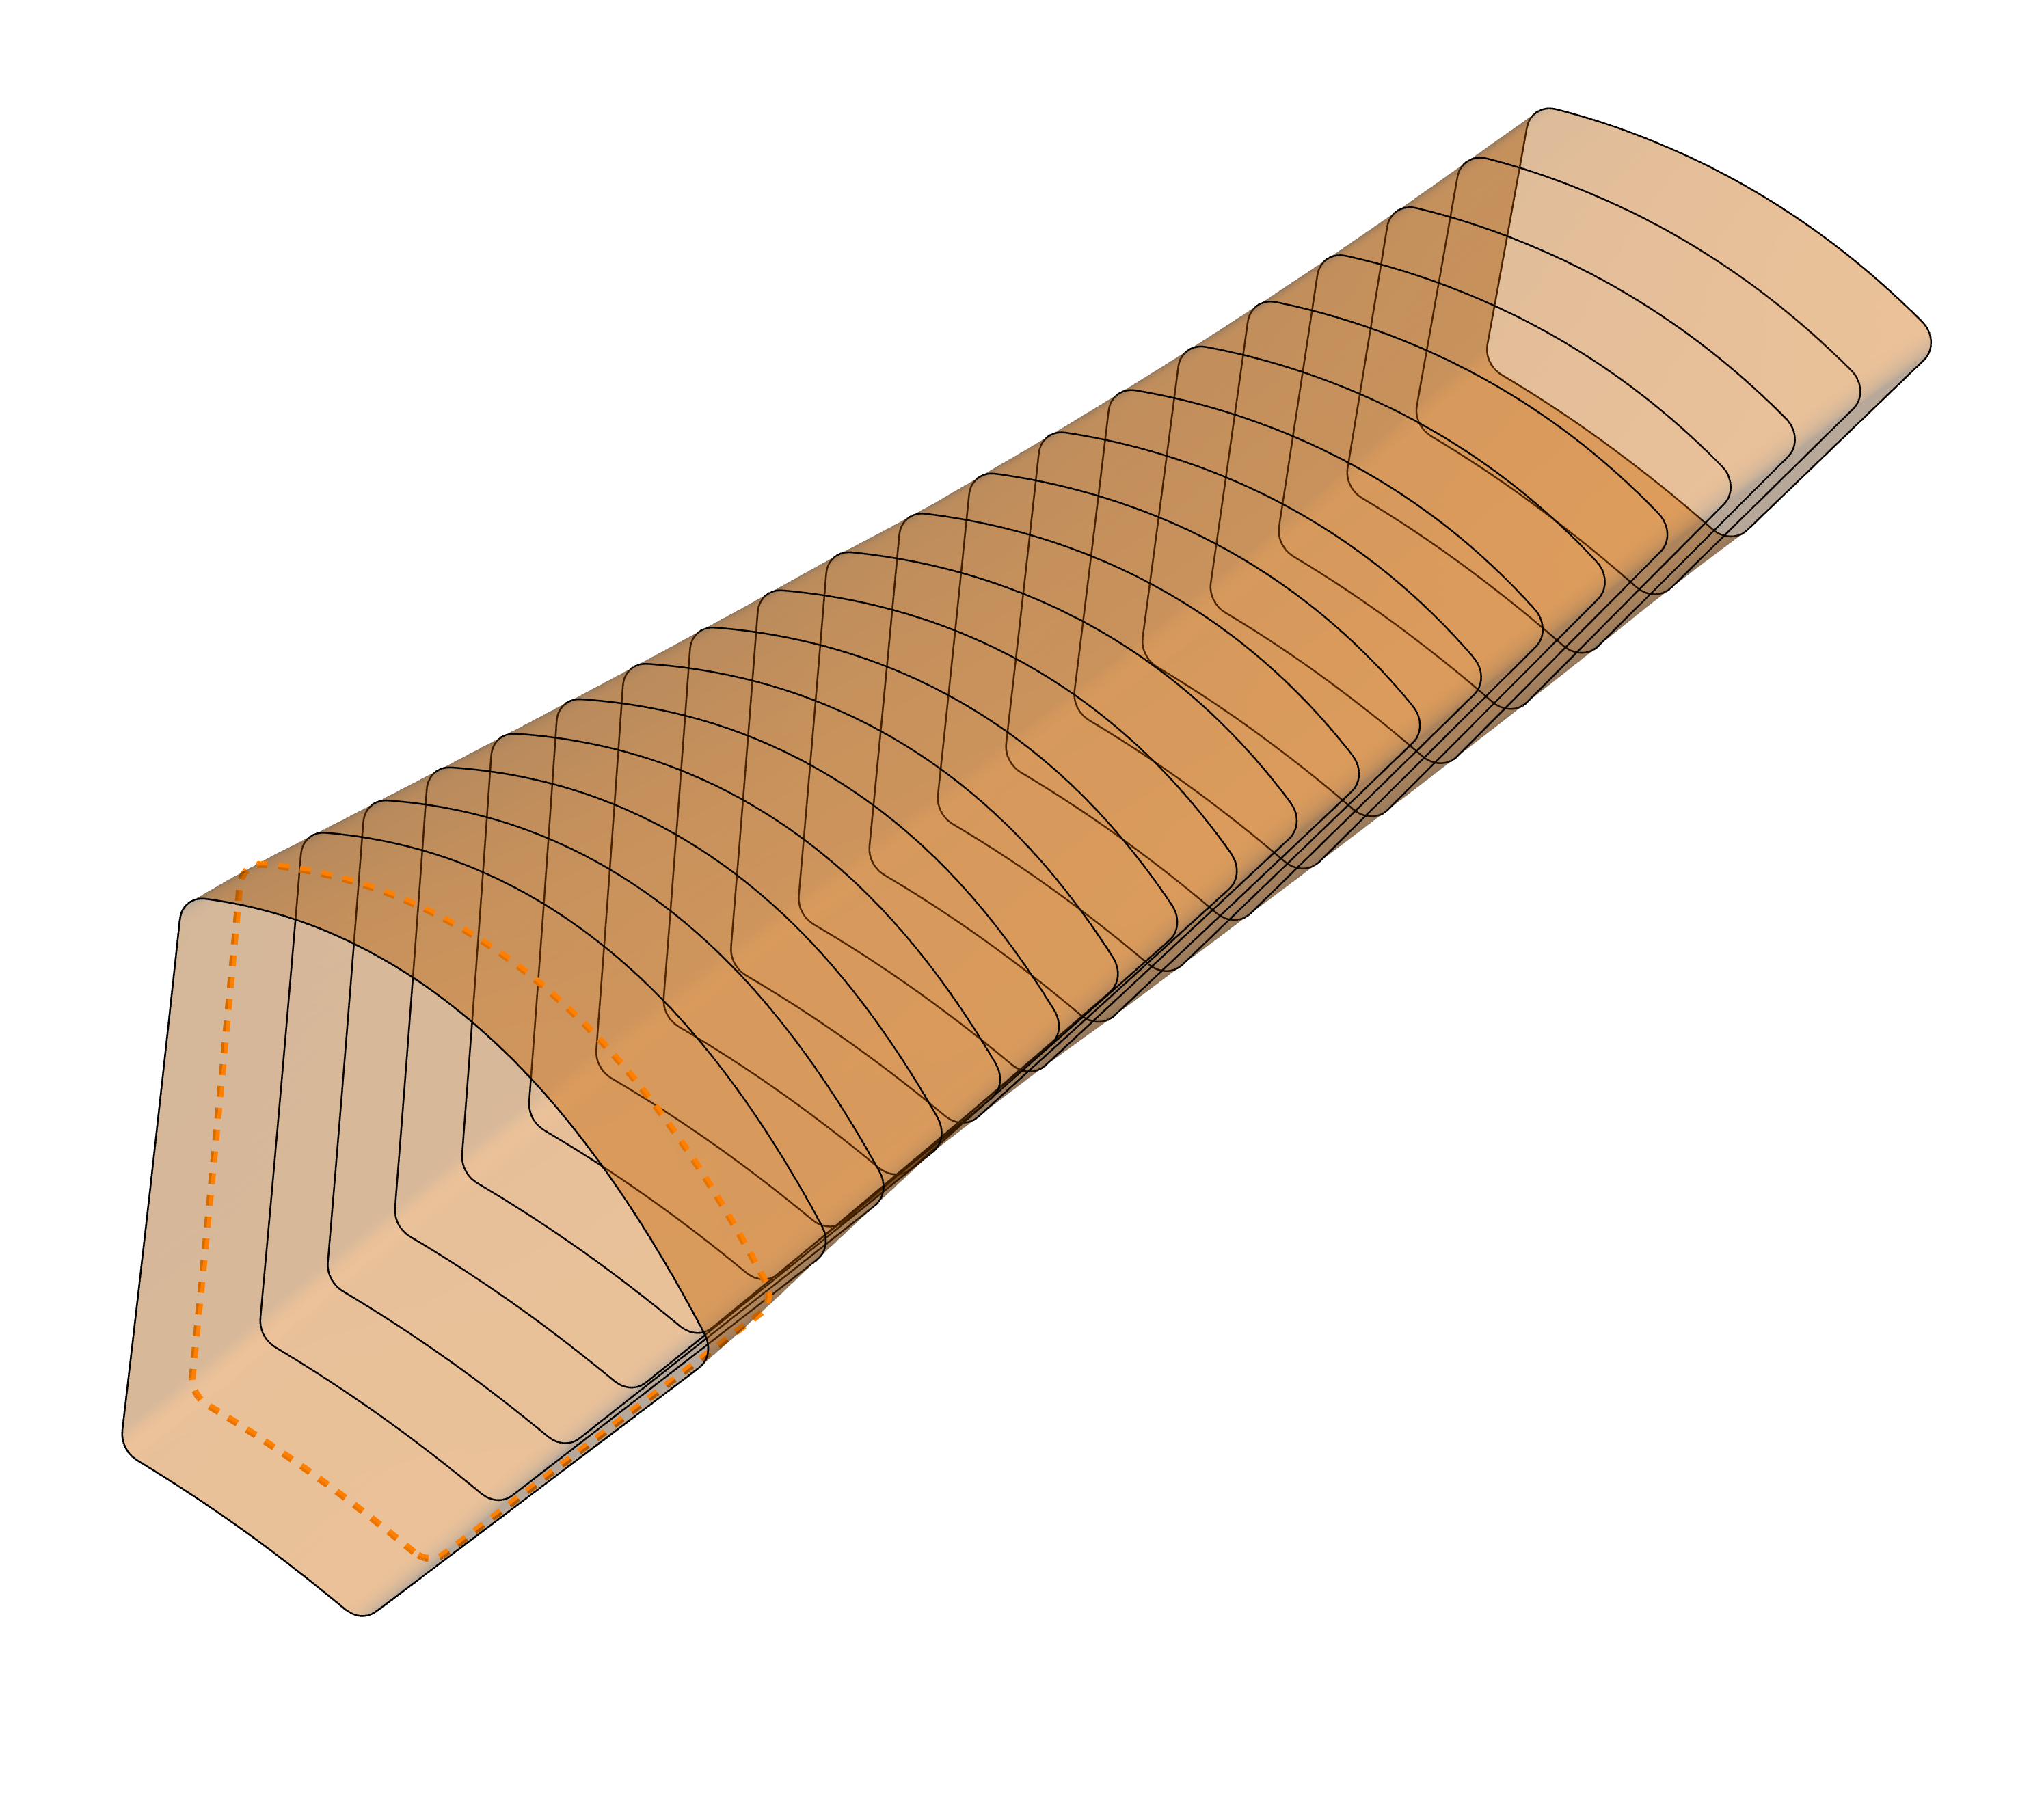
\includegraphics[width=\textwidth]{../tec/chambers/114.png}
			\caption{A single chamber.}
		\end{subfigure}
		\begin{subfigure}{.44\textwidth}
			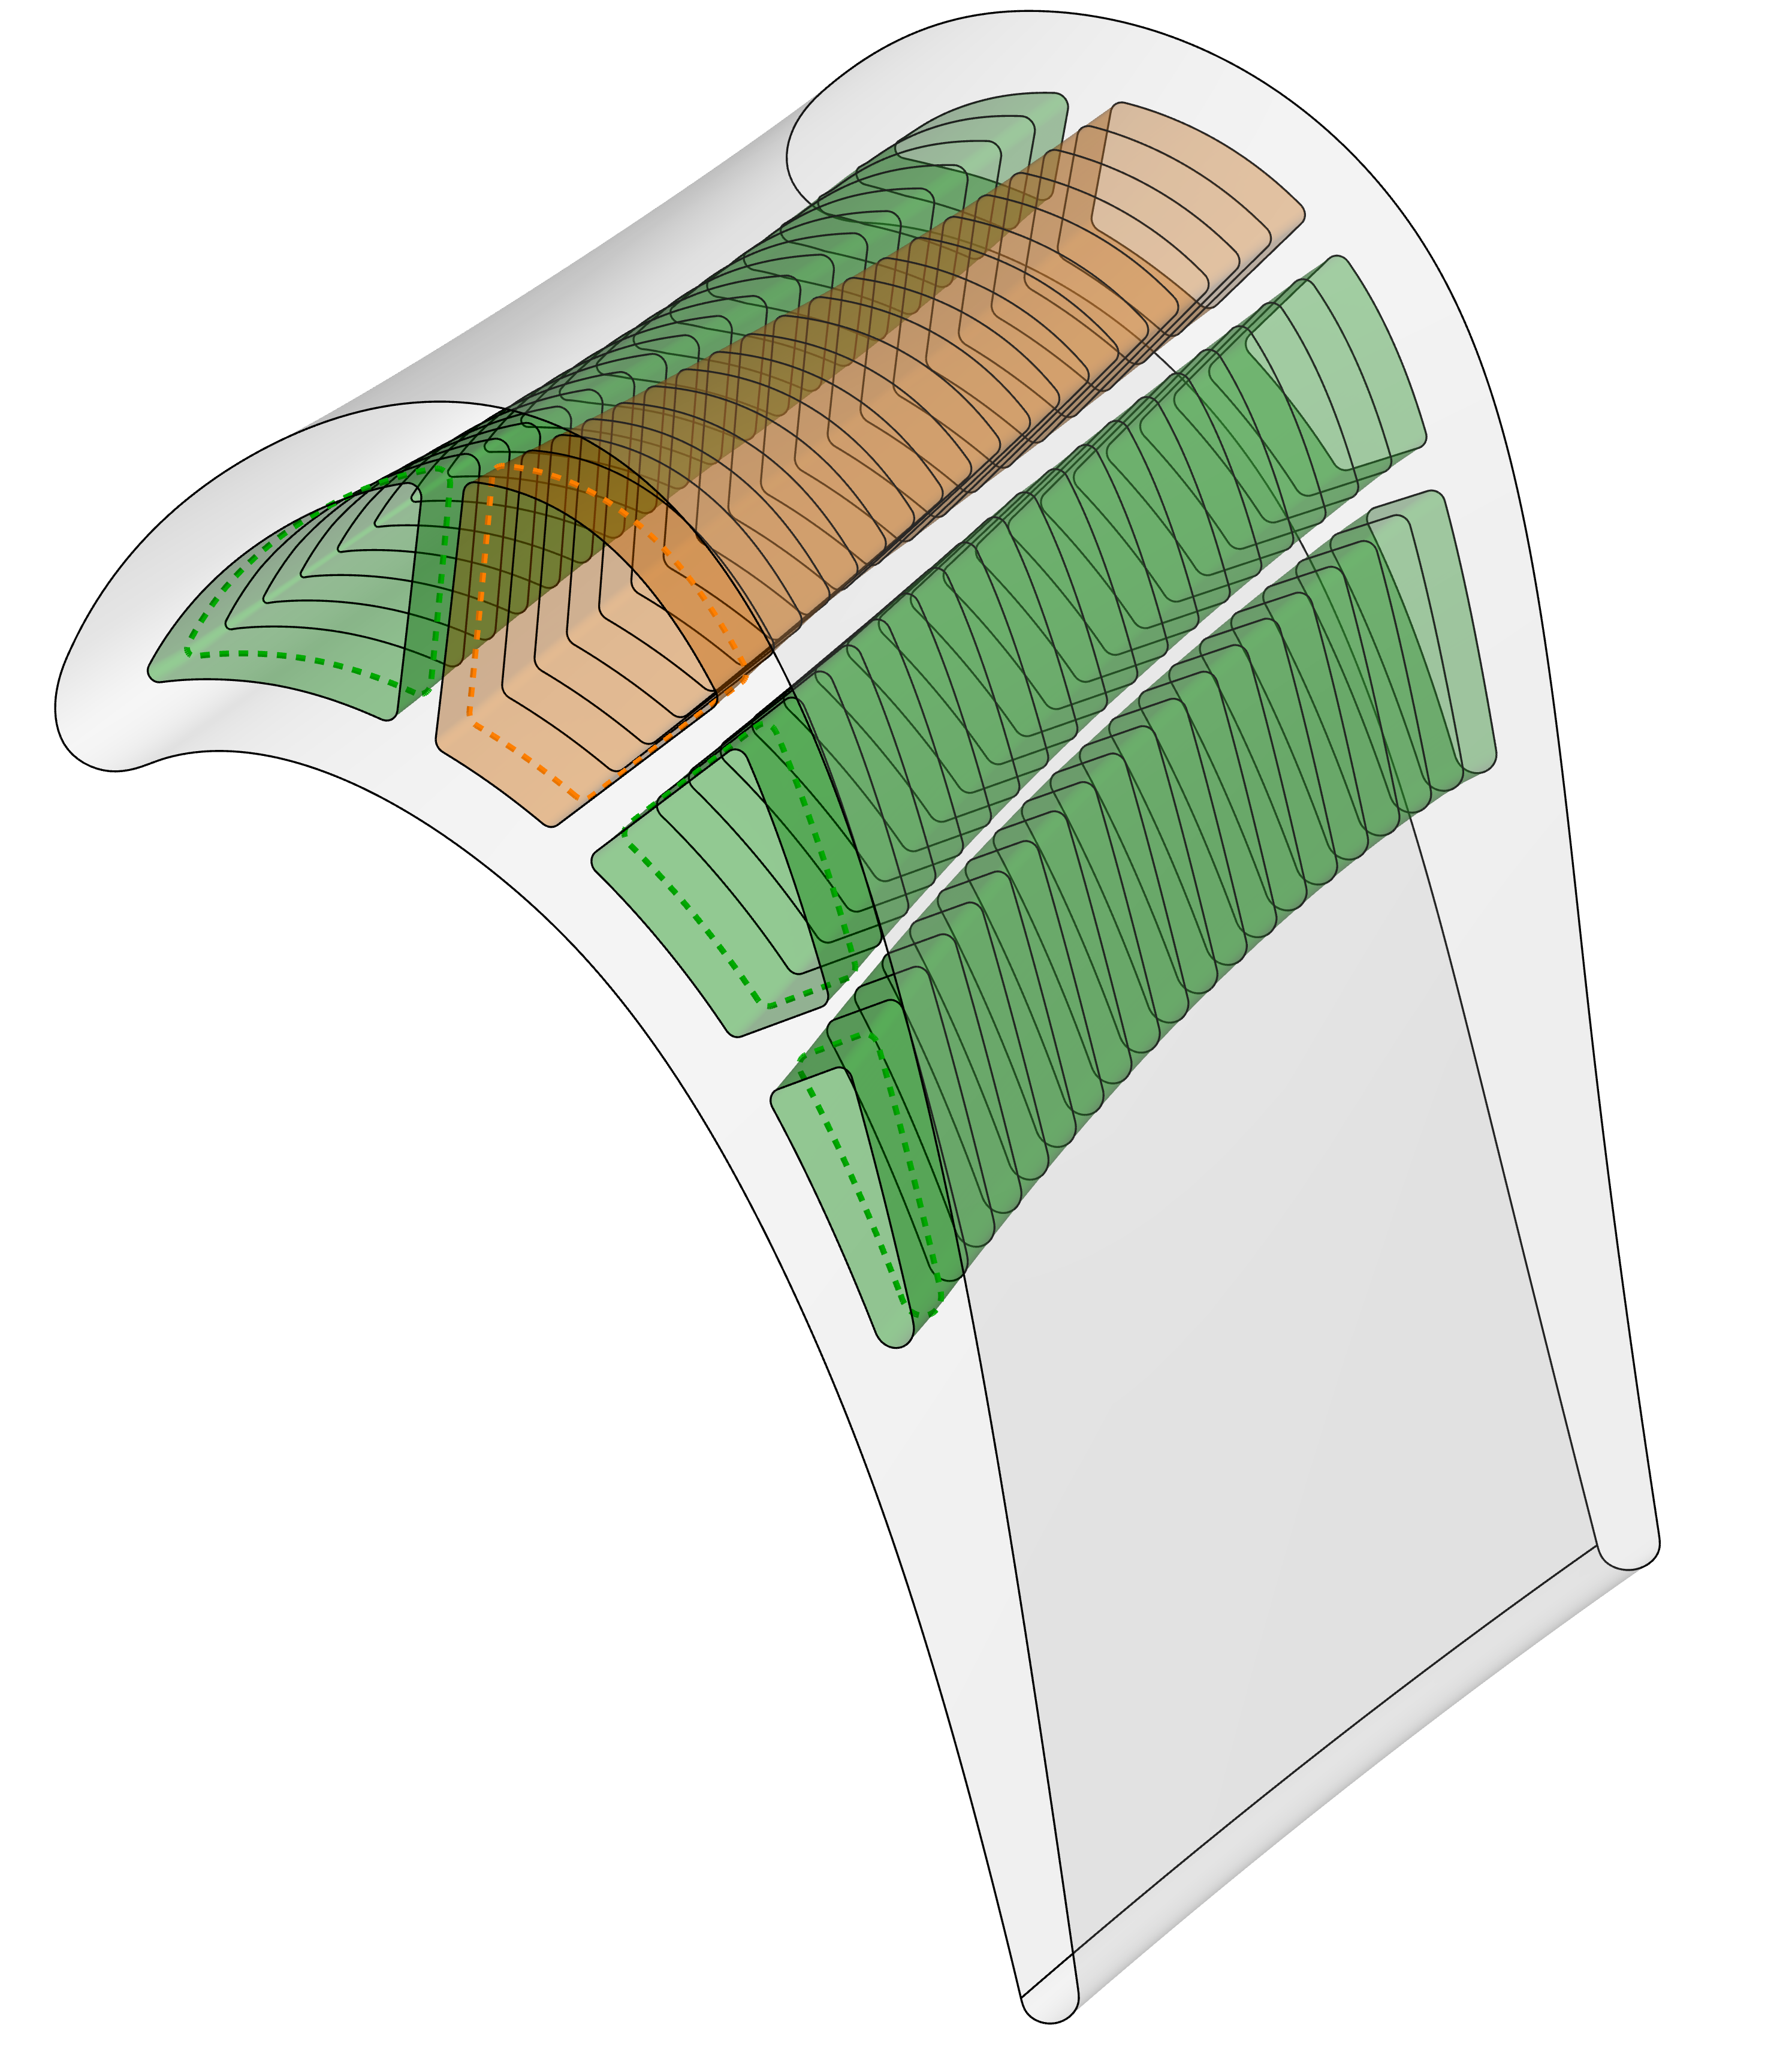
\includegraphics[width=\textwidth]{../tec/chambers/111.png}
			\caption{Four chambers.}
		\end{subfigure}
		\caption{Skinned chamber surfaces.}
		\label{fig:skinned_chambers}
	\end{figure}
	
	After connecting and trimming the offset curves using the methods in Section \ref{sec:offsetcurves}, we are left with four trimmed offset curves that intersect at their end points. We apply the fillet curve method presented in Section \ref{sec:filletcurves} between neighboring chamber-delimiting curves. The offsetting, trimming and fillet creation steps can be seen in Figure \ref{fig:chamber_shrinking}.

	As described in Section \ref{sec:mrtheta}, we can use the inverse coordinate transformation from the $(m, r\theta)$ stream surface coordinate system to the Cartesian coordinate system and use surface skinning to create chamber surfaces. Figure \ref{fig:skinned_chambers} shows an exemplary result of this procedure.

\subsection{Turns}
	As mentioned before, a turn lets coolant flow between two chambers. Notice that the presented method, unlike the construction of chambers, takes place in Cartesian coordinates.

	\begin{figure}[H]
		\centering
		\begin{subfigure}{.62\textwidth}
			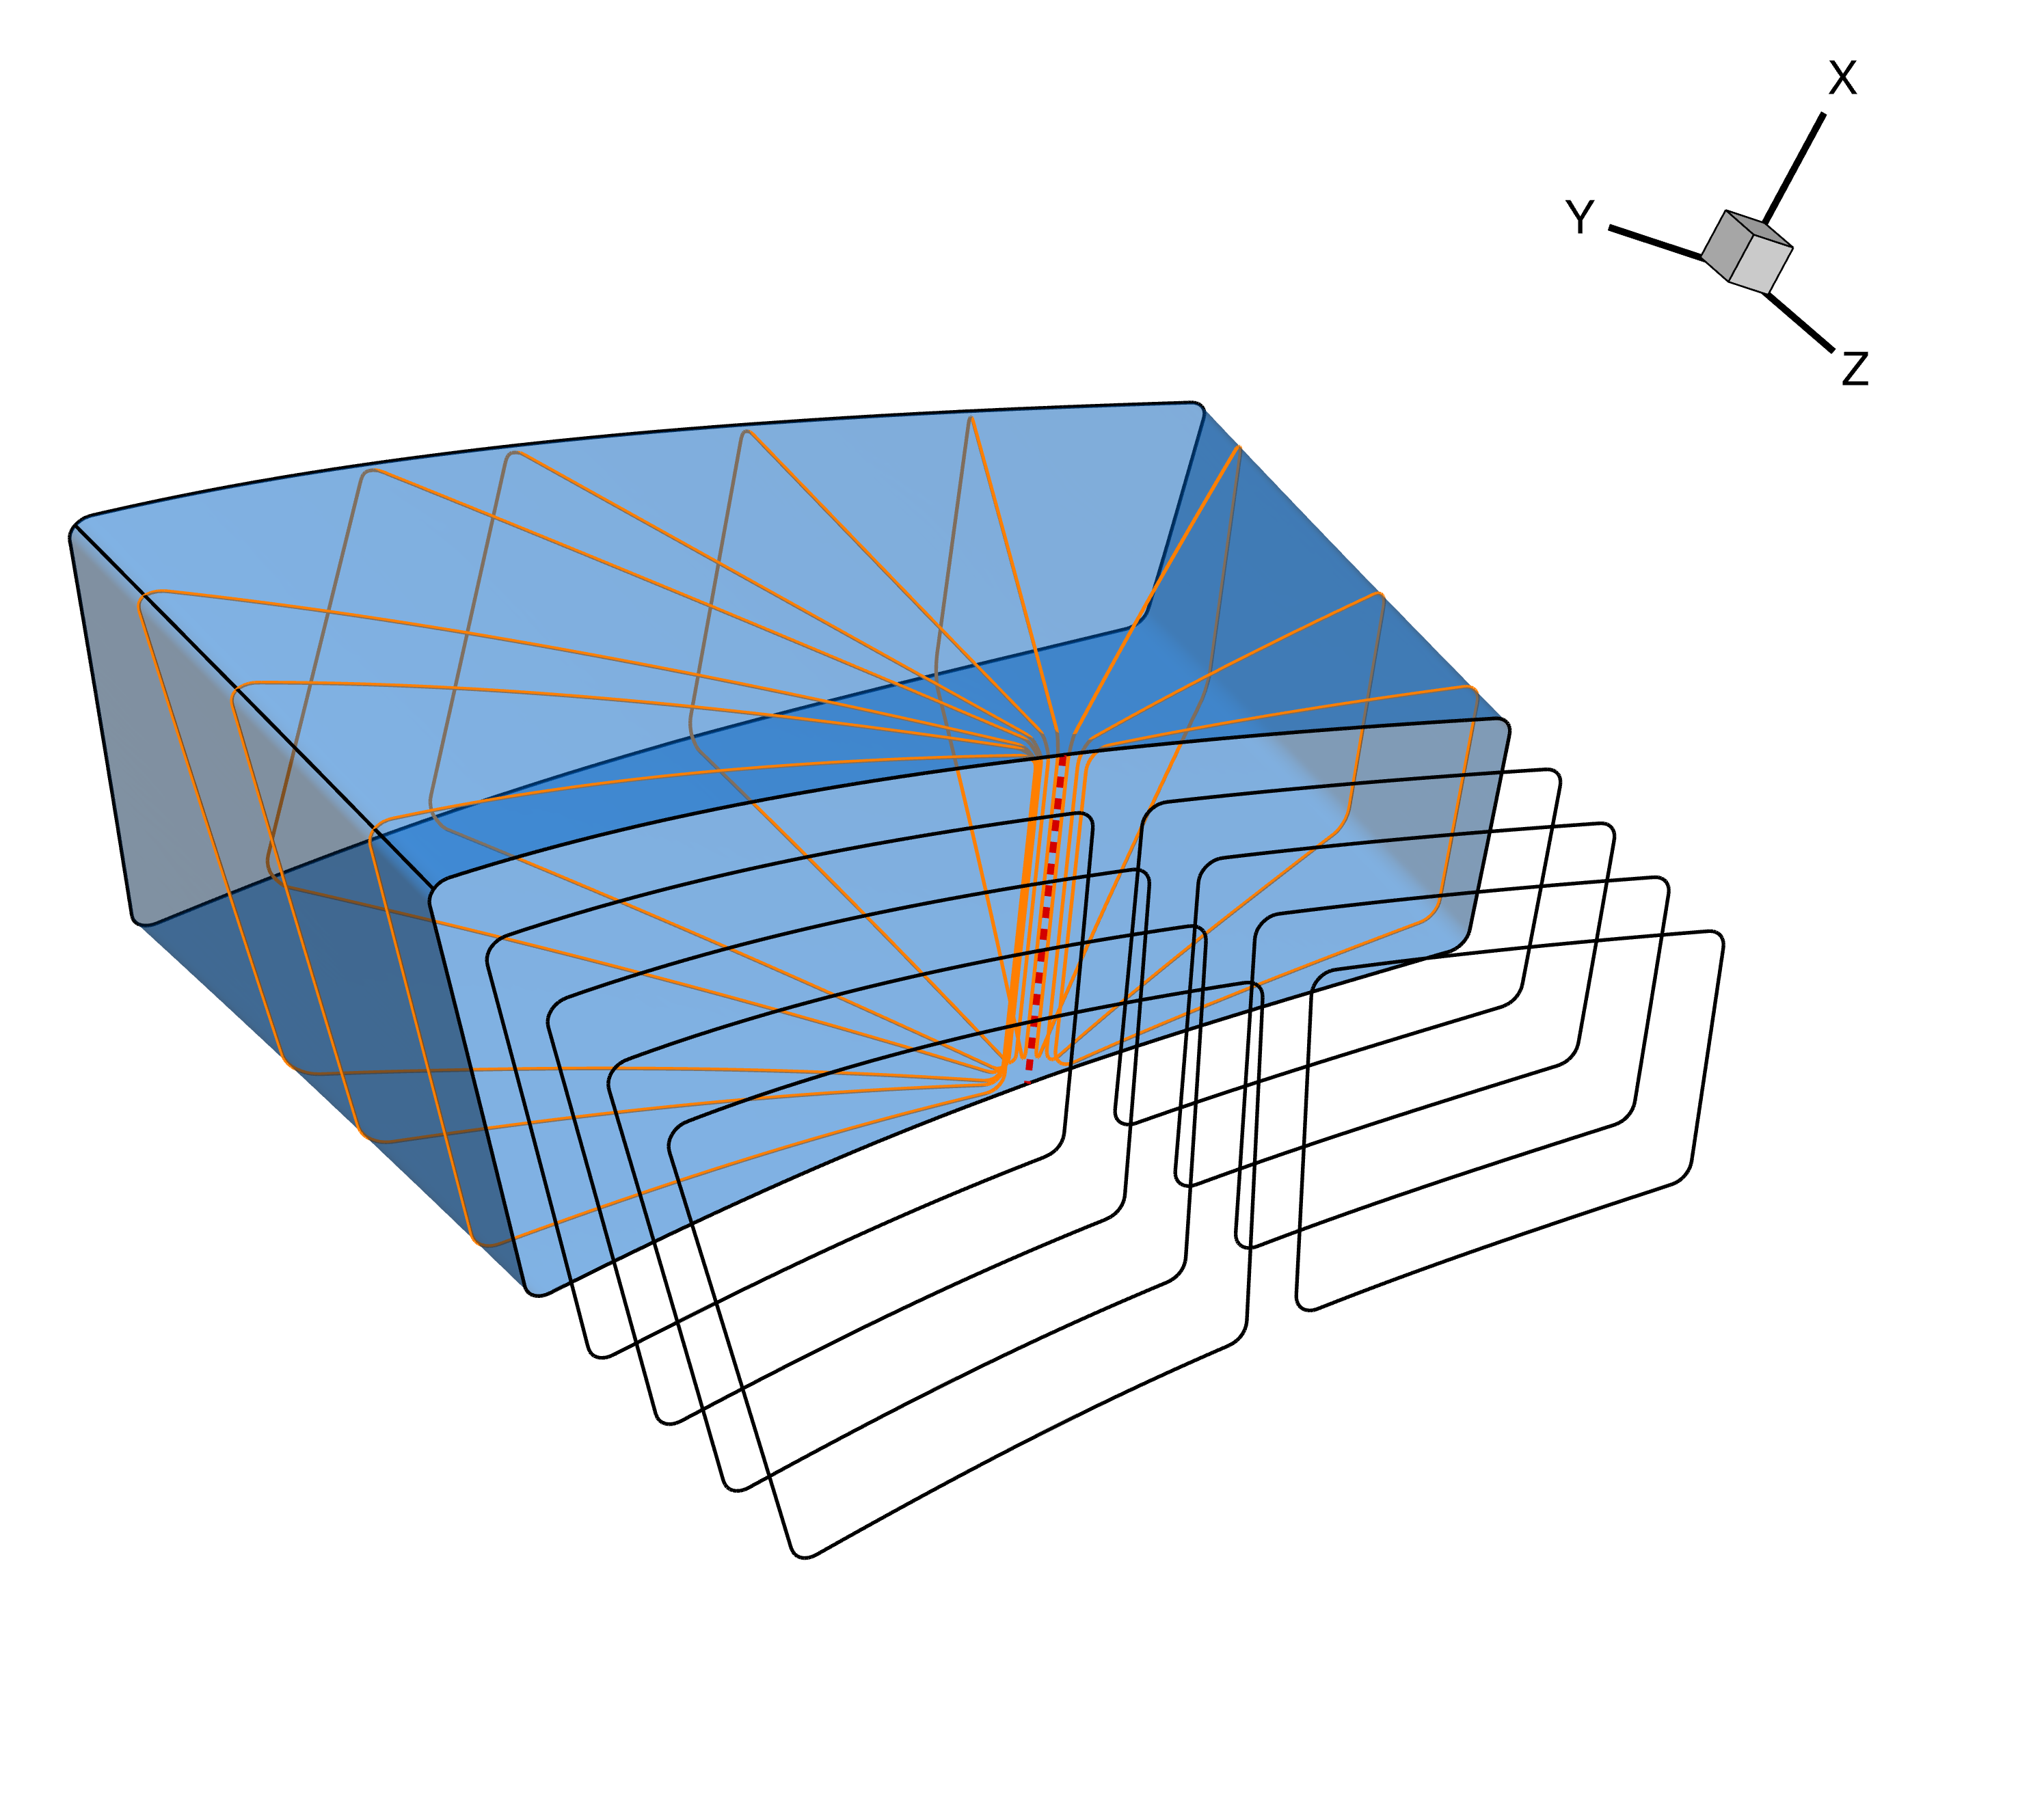
\includegraphics[width=\textwidth]{../tec/channel/11.png}
		\end{subfigure}
		\begin{subfigure}{.37\textwidth}
			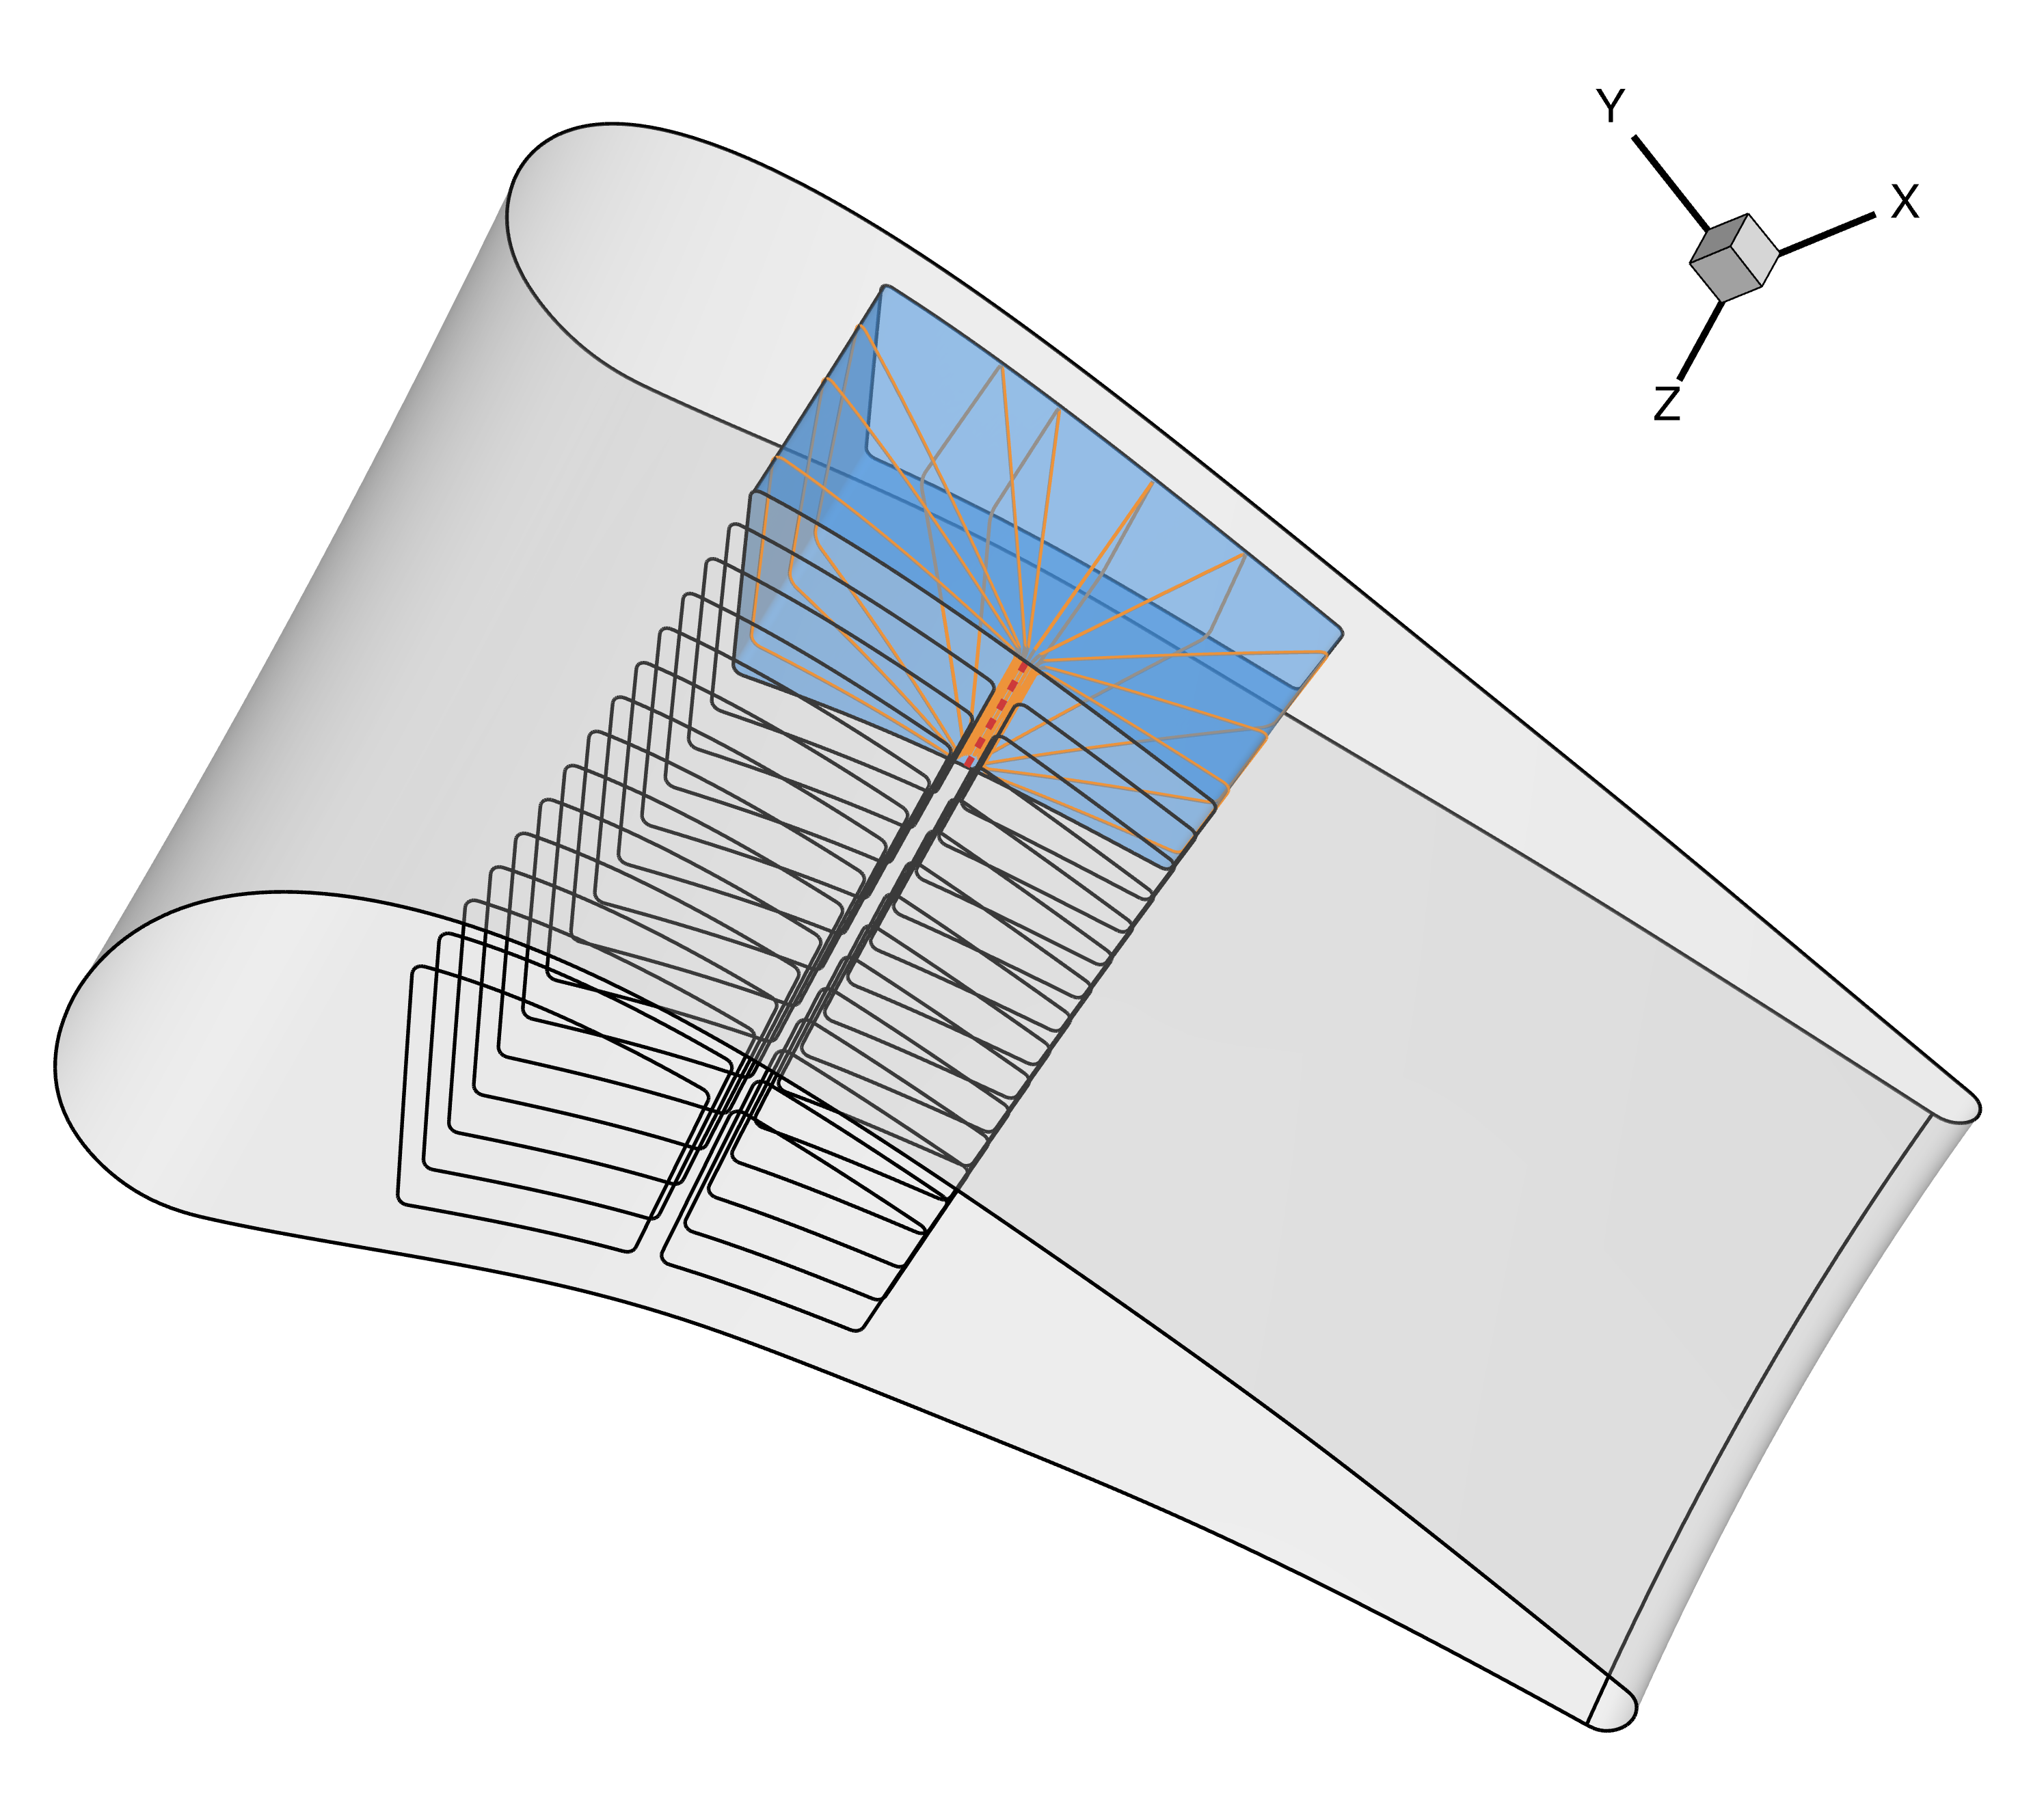
\includegraphics[width=\textwidth]{../tec/channel/12.png}
			\vspace{1.2cm}
		\end{subfigure}
		\caption{Construction of a turn. The red dashed line represents the axis around which the turn is constructed. The black curves are the chamber profiles which were calculated in Section \ref{sec:chambers}. The blue surface is the combination of two neighboring chambers. The orange curves are intersections of planes that contain the turn axis and the combined chamber.}
	\end{figure}

	First, we construct the combined chamber, for which the two chambers that shall be connected by the turn are specified. The intermediate surface partitions are removed, and the suction and pressure sides of the two chambers are connected differentiably by inserting control points. For this purpose, the user specifies a lower bound $v_L$ and an upper bound $v_U$, between which the combined chamber (and therefore the turn) is constructed.

	Next, the turn axis is constructed. The wall input of the intermediate wall (see Section \ref{sec:chambers}) has a Cartesian representation as a surface. The $v_L$-isoparametric curve end points of this wall surface are connected with a straight line. This yields the turn axis. Using the turn axis, we can construct a set of planes which intersect the turn axis. A set of angles (relative to the intermediate wall) are specified as an input. The combined chamber is partitioned into a suction and a pressure side.

	We use Algorithm \ref{alg:surfplaneintersection} to find the intersection of these planes and the suction and pressure side of the combined chamber, yielding two curves for each plane. The intersection curves start at the turn axis and end at the suction or pressure side boundary, respectively. The start points of these curves do not intersect, but both start points lie on the turn axis. We connect these points using a straight line, which lies inside the turn axis. If the end points do not intersect, we also connect them using a straight line.

	Since all of these curves (including the straight lines, which are represented as curves within CoolingGen) are planar by construction, we can use two-dimensional operations to offset, trim and add fillets. Since CoolingGen performs two-dimensional operations on the $(x,y)$ plane, the curves have to be rotated.

	To ensure a differentiable connection between the chambers, the axis-aligned curve is offset. The size of the offset is given by the linear interpolation in terms of the angle between the wall thickness on the leading and on the trailing side. Similar to the procedure in \ref{sec:chambers}, the pressure- and suction-sided curves are then trimmed accordingly and fillets are added between them.

	\begin{figure}[H]
		\centering
		\begin{subfigure}{.49\textwidth}
			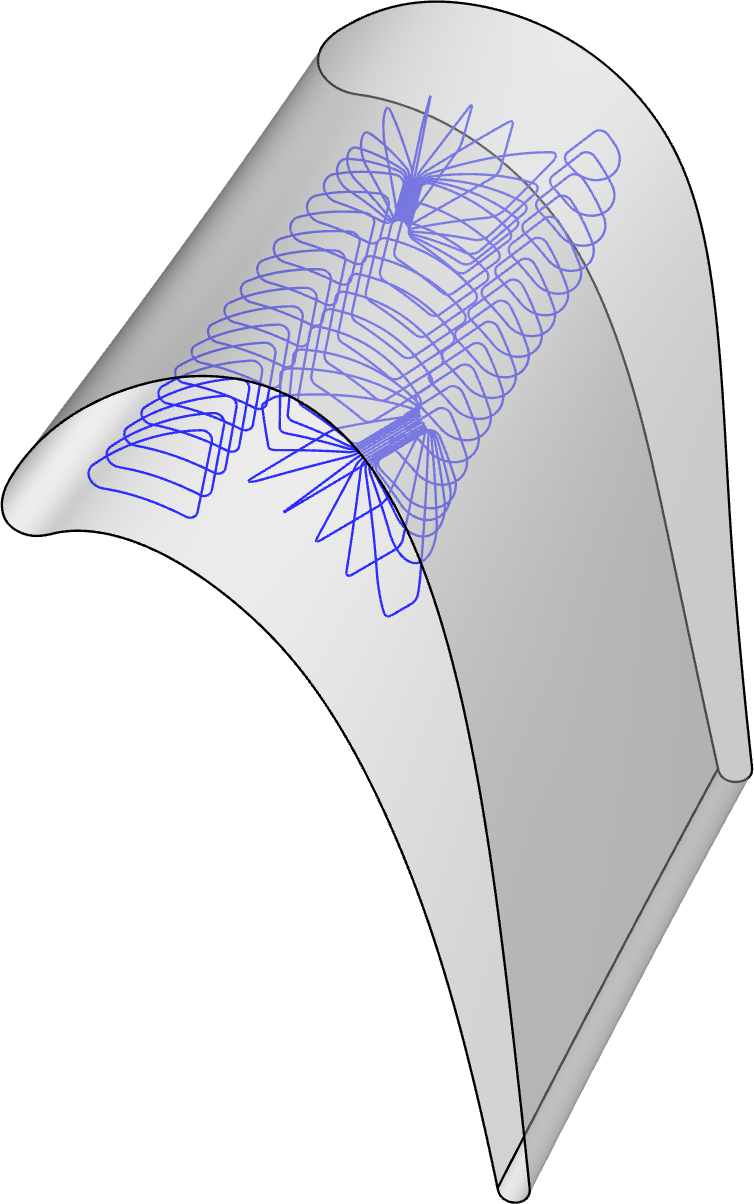
\includegraphics[width=\textwidth]{../tec/channel/13.png}
			\caption{Profile curves.}
		\end{subfigure}
		\begin{subfigure}{.49\textwidth}
			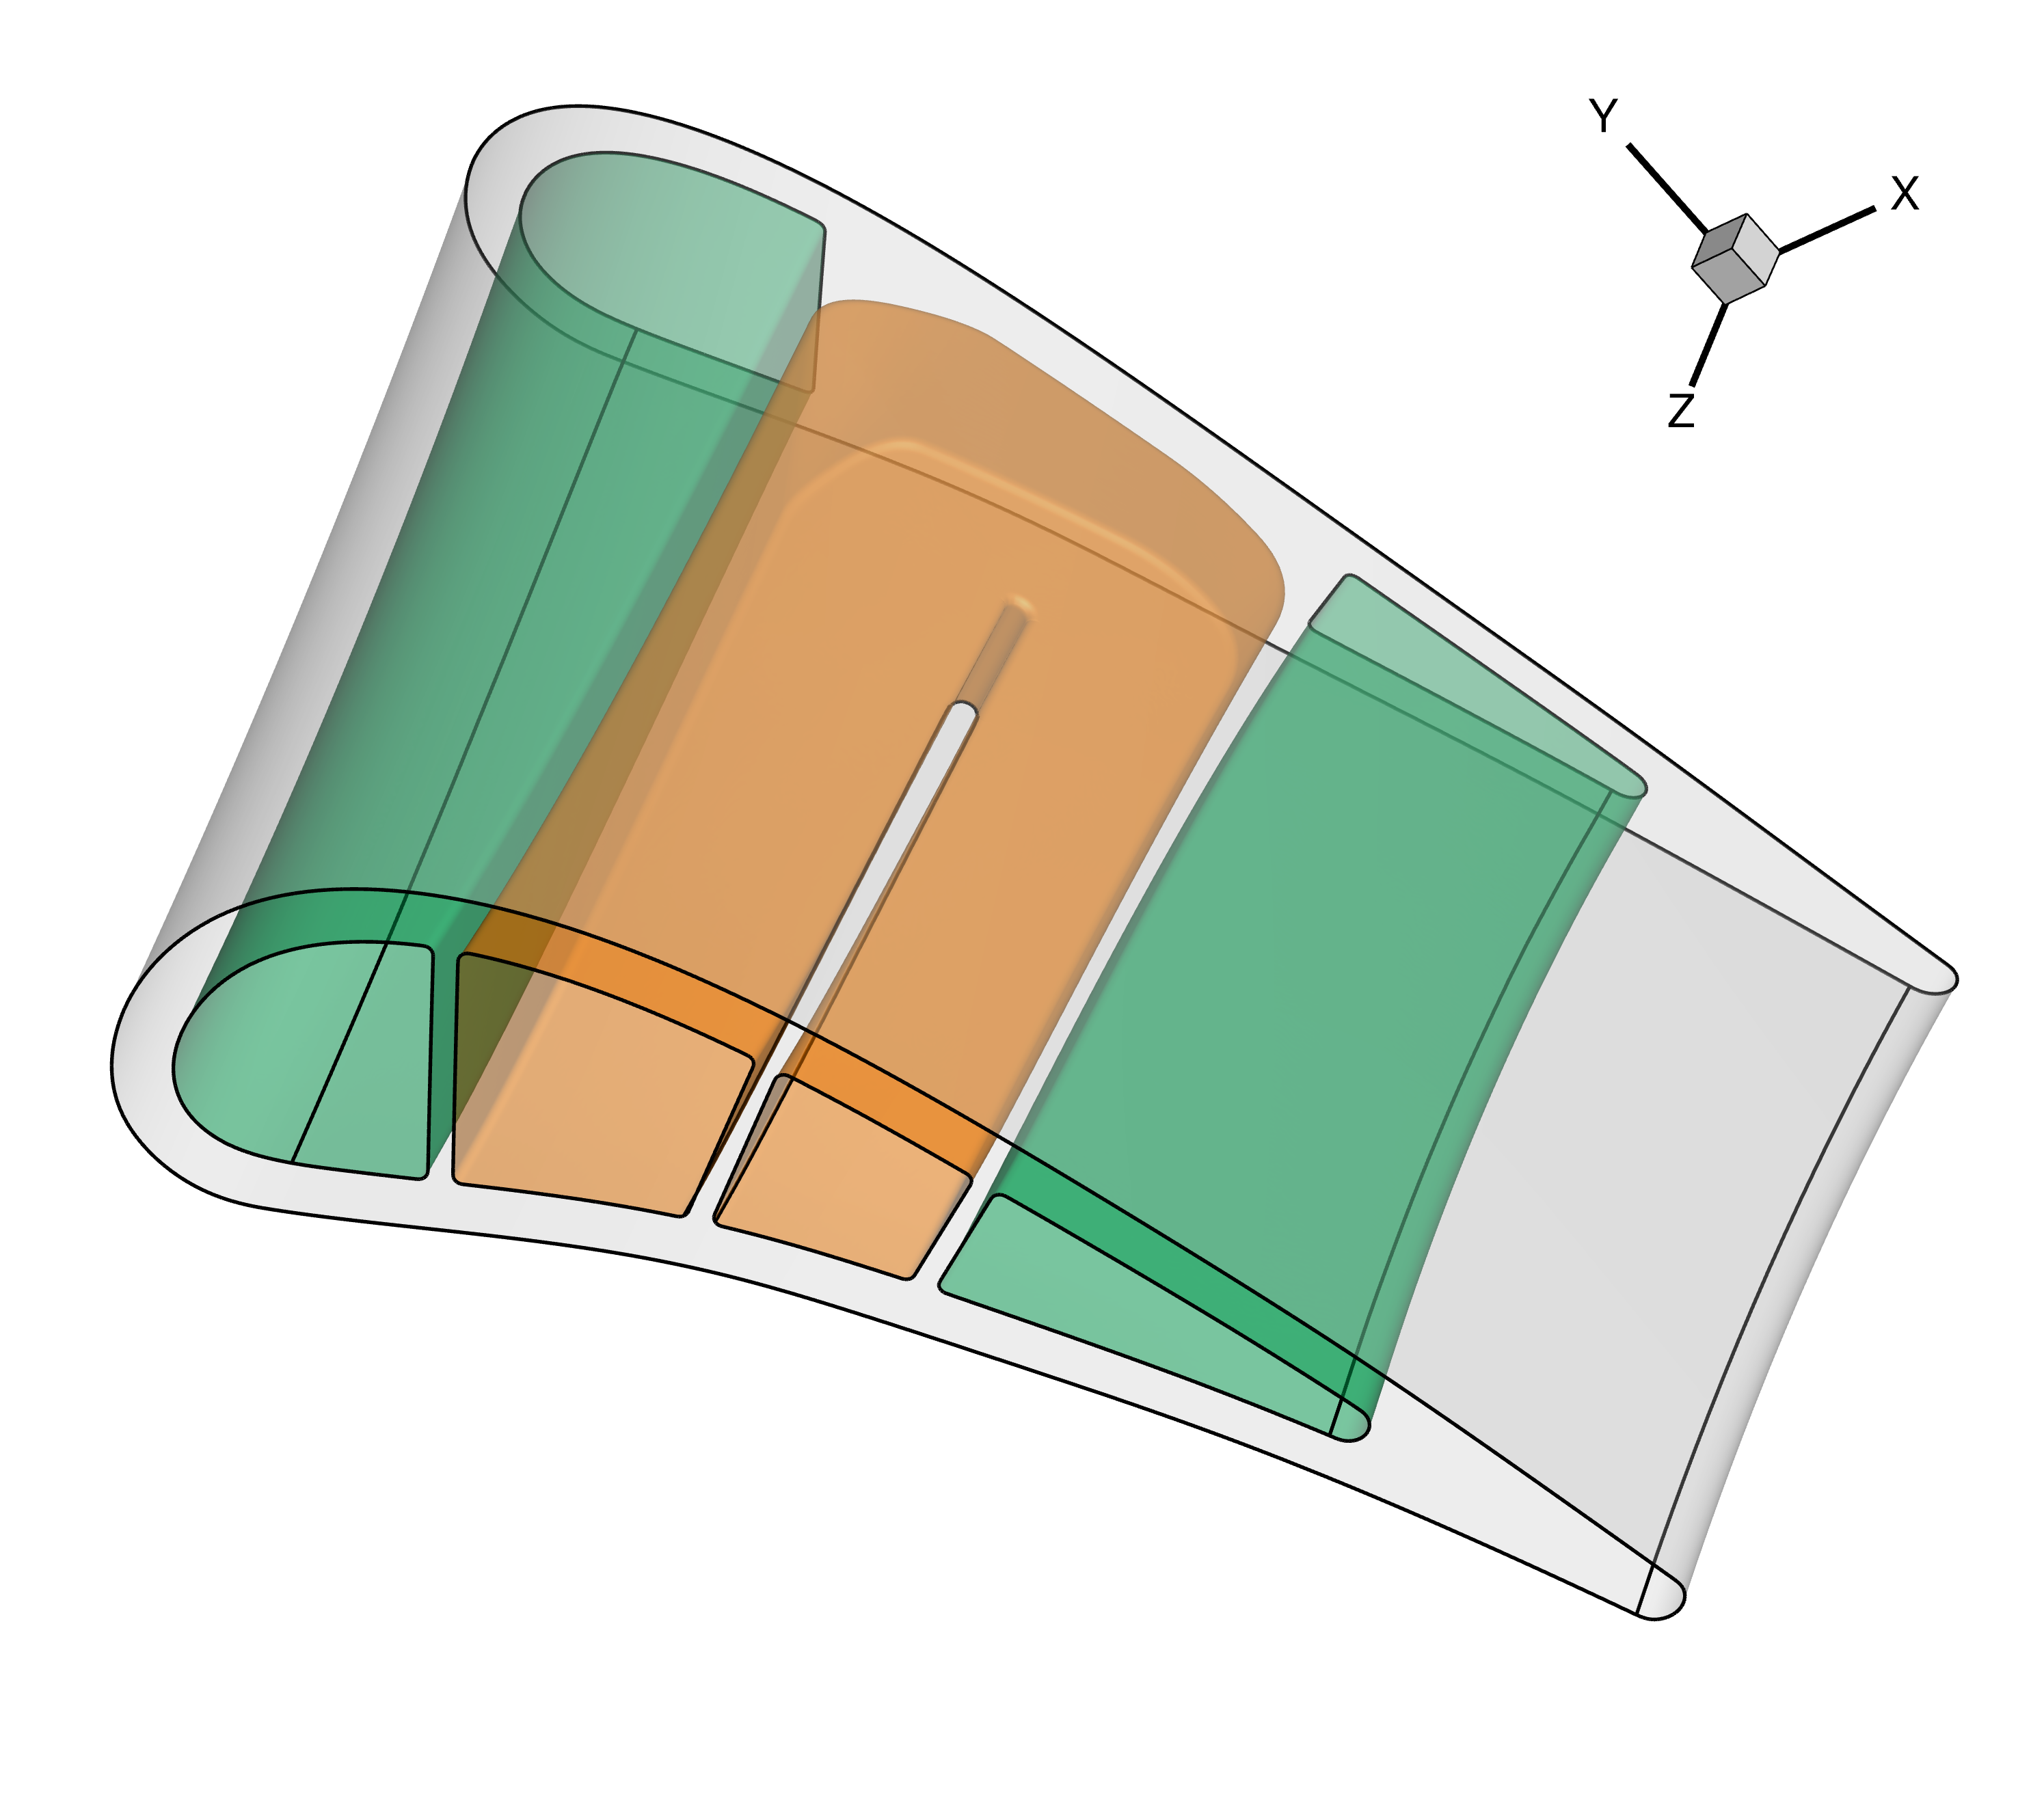
\includegraphics[width=\textwidth]{../tec/channel/14.png}
			\caption{Surfaces.}
		\end{subfigure}
		\caption{Three cooling channels.}
	\end{figure}

	After rotating the planar curves back from the $(x,y)$-plane onto their original plane, we once again use skinning to combine the planar curves to turn surfaces. However, these turn surfaces do not contain the chambers. As mentioned at the beginning of this chapter, the coherent combination of turns and chambers is called channel. To construct a channel from turns and chambers, we find the profiles and planar curves that belong to the channel. We align their start points and direction by shifting the parameter space in the following way.

	Given a parametric curve $\gamma(t)$ with $t \in [0,1]$, we can align the curve by applying the map
		$$ \Phi(s, \sigma, t): [0,1] \rightarrow [0,1] \quad t \mapsto (s+\sigma t+1) \textrm{ mod } 1, $$
	to the input parameter $t$, where $s \in [0,1]$ is the parametric shift, $\sigma \in \{1, -1\}$ is the curve direction, and $\textrm{mod}$ is the modulus operator. Using this map and Algorithm \ref{alg:pointinversion}, we can align two curves at a point.

	The reason why this is necessary may become apparent through Figure \ref{fig:chambers_vs_turns}. The black curve on the channel represents the $u=0$ isoparametric curve of the channel surface. As can be seen, this curve switches position throughout the turn. In the first chamber, the curve lies on the leading edge side, then on the trailing edge side and then once again on the leading edge side. The turns show the same behavior. In the turn on the leading edge side, the curve lies on the far side of the turn, whereas in the turn on the trailing edge side, the curve lies on the near side of the turn.

\section{Film Cooling Holes}\label{sec:filmcooling}
	In this section, the construction of film cooling holes is presented.

	\begin{figure}[H]
		\centering
		\begin{subfigure}{.15\textwidth}
			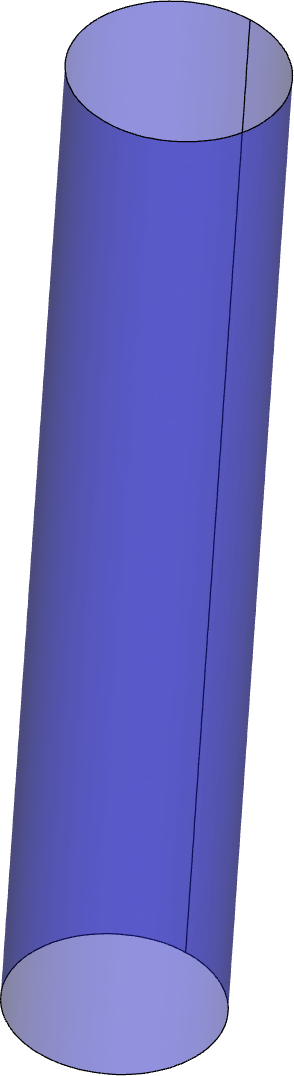
\includegraphics[height=6cm]{../tec/holes/16.png}
			\vspace{1.5cm}
			\caption{Cylindrical.}
		\end{subfigure}
		\phantom{aa}
		\begin{subfigure}{.19\textwidth}
			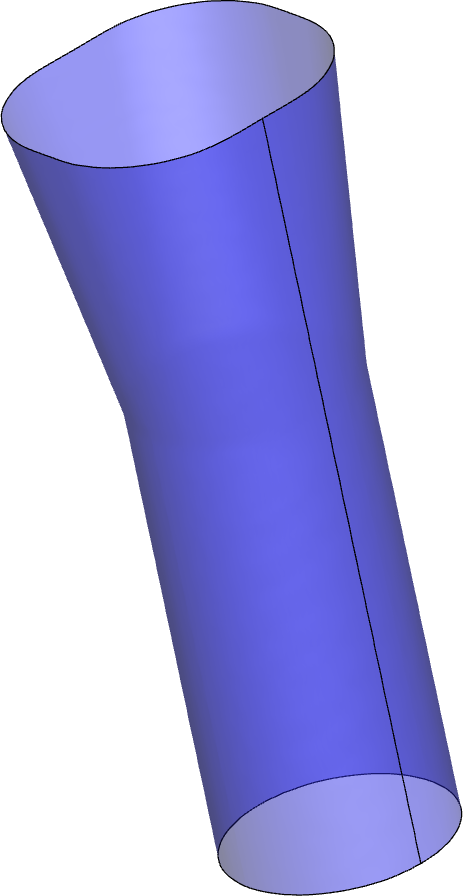
\includegraphics[height=6cm]{../tec/holes/15.png}
			\vspace{1.1cm}
			\caption{Fan shaped.}
		\end{subfigure}
		\begin{subfigure}{.55\textwidth}
			\includesvg[width=\textwidth]{../python/fanshapedCurveDefinition}
			\caption{$f_\textrm{circular}$ (orange) and $f_\textrm{fan shaped}$ (blue).}
		\end{subfigure}
		\caption{Film cooling holes and their delimiting curves.}
		\label{fig:filmholes}
	\end{figure}

	The general shape of a film cooling hole is described using two delimiting curves which are closed and a transitional $v$-parameter, which we will call $v_\textrm{transition} \in [0,1]$. CoolingGen currently supports two types of delimiting parametric curves, but can be extended to provide a multitude of such curves. The currently supported curves are the circular curve
		$$ f_\textrm{circular}(t) =
			\begin{pmatrix}
				r \cos 2\pi t \\
				r \sin 2\pi t
			\end{pmatrix},
		$$
	for a given radius $r$, and the fan shaped curve
		$$ f_\textrm{fan shaped}(t) = 
			\begin{cases} 
				\begin{pmatrix}
					r\\
					0 
				\end{pmatrix}
				& \textrm{ if } t \in \{0, 1\},\\[1.1em]
				
				\begin{pmatrix}
					0 \\
					b
				\end{pmatrix}
				& \textrm{ if } t = \frac{1}{4},\\[1.1em]

				\begin{pmatrix}
					r - 2d \\
					0
				\end{pmatrix}
				& \textrm{ if } t = \frac{1}{2},\\[1.1em]

				\begin{pmatrix}
					0 \\
					-b
				\end{pmatrix}
				& \textrm{ if } t = \frac{3}{4},\\[1.1em]				
			\end{cases}
			\quad\textrm{or}\quad
			\begin{cases} 
				\begin{pmatrix}
					r \cos 2\pi t \\
					r \sin 2\pi t + (b-r)
				\end{pmatrix}
				& \textrm{ if } t \in (0, \frac{1}{4}),\\[1.1em]

				\begin{pmatrix}
					r \cos 2\pi t - 2(d-r) \\
					r \sin 2\pi t + (b-r)
				\end{pmatrix}
				& \textrm{ if } t \in (\frac{1}{4}, \frac{1}{2}),\\[1.1em]

				\begin{pmatrix}
					r \cos 2\pi t - 2(d-r)\\
					r \sin 2\pi t - (b-r)
				\end{pmatrix}
				& \textrm{ if } t \in (\frac{1}{2}, \frac{3}{4}),\\[1.1em]

				\begin{pmatrix}
					r \cos 2\pi t \\
					r \sin 2\pi t - (b-r)
				\end{pmatrix}
				& \textrm{ if } t \in (\frac{3}{4}, 1),\\[1.1em]
			\end{cases}
		$$
	where $r > 0$ is the corner radius, $b > 0$ is the height, $d > 0$ the width and $t \in [0,1]$. Both of these curves can be seen in Figure \ref{fig:filmholes}.

	\begin{figure}[H]
		\centering
		\begin{subfigure}{.35\textwidth}
			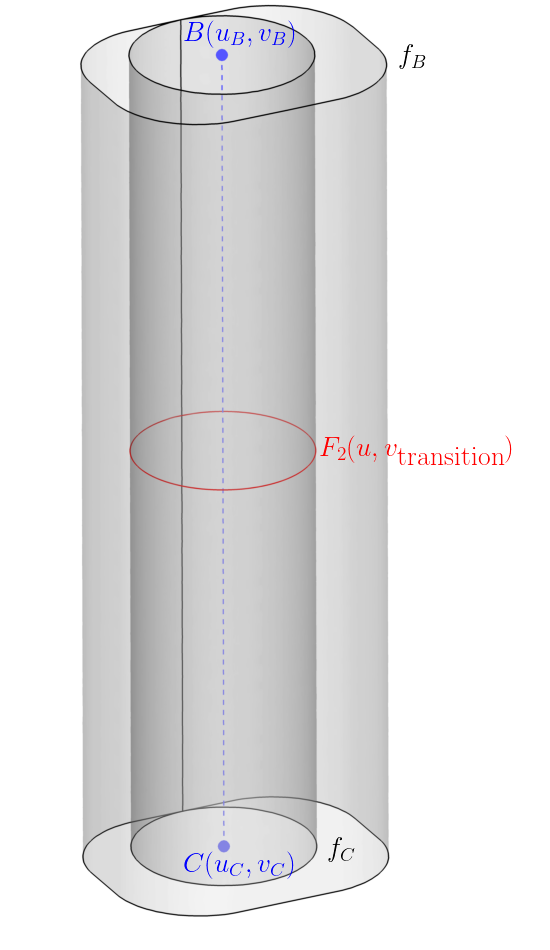
\includegraphics[width=\textwidth]{../tec/holes/00edit.png}
			\caption{Extrusion surfaces $F_1$ and $F_2$.}
		\end{subfigure}
		\begin{subfigure}{.35\textwidth}
			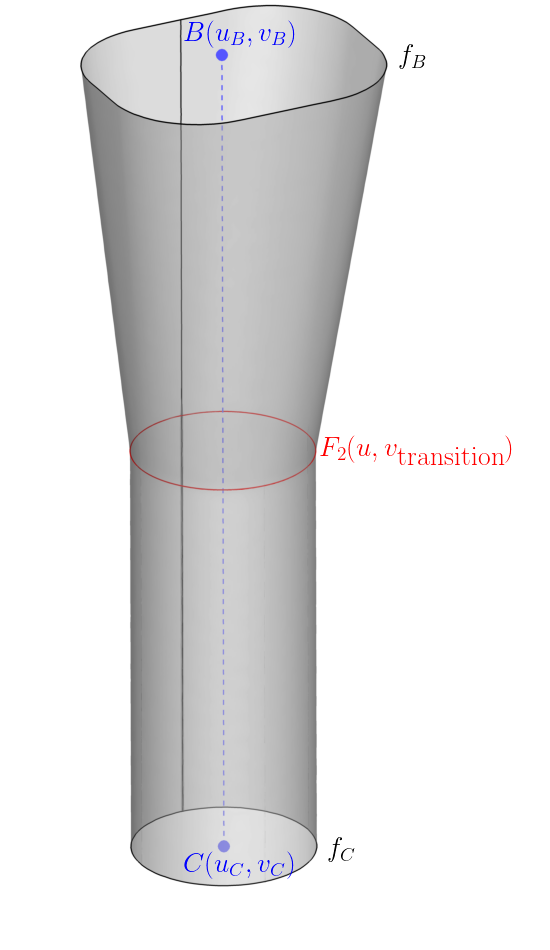
\includegraphics[width=\textwidth]{../tec/holes/01edit.png}
			\caption{Film cooling hole $F^{(v_\textrm{transition})}$.}
		\end{subfigure}
		\caption{Construction of a film cooling hole.}
		\label{fig:filmcooling_construction}
	\end{figure}

	To construct a surface from a delimiting curve $f$, we canonically embed the two-dimensional curves into three-dimensional space using the map
		$$ E: \mathbb{R}^2 \rightarrow \mathbb{R}^3, \quad (x, y) \mapsto (x, y, 0). $$
	We also require a line segment $L_{P_B,P_C}$ between two points $P_B, P_C \in \mathbb{R}^3$.
	The curve $E(f)$ lies in the $(x,y)$-plane that has the normal vector $N_{(x,y)} = (0, 0, 1)$. We construct the rotation matrix $R \in \mathbb{R}^{3 \times 3}$ that rotates $N_{(x,y)}$ onto the direction $(P_C-P_B)$ of the line segment $L_{P_B,P_C}$ by finding the angle between $(P_C-P_B)$ and $N_{(x,y)}$. The rotation axis is given by the cross product $(P_C-P_B) \times N_{(x,y)}$. Using the rotation matrix $R$, we can rotate $E(f)$ to calculate $RE(f)$. We can translate $RE(f)$ to the start and end points of $L_{P_B,P_C}$ to calculate two curves
		$$ f_B(t) := P_B+RE(f(t)) \quad\textrm{and}\quad f_C(t) = P_C+RE(f(t)), $$
	for $t \in [0,1]$.
	For all $v \in [0,1]$, we can linearly interpolate between $f_B(u)$ and $f_C(u)$ for each $u \in [0,1]$ to find the surface 
		$$F(u,v) = (1-v)\,f_B(u) + v\,f_C(u).$$
	We call the surface $F(u,v)$ the extrusion of $f$ along $L_{P_B,P_C}$. Two extrusion surfaces can be seen in Figure \ref{fig:filmcooling_construction}.

	Setting a value $v_\textrm{transition} \in [0,1]$, we can combine two extrusion surfaces of different curves $f_1$ and $f_2$ along the same line segment. This will yield the characteristic shape of the film cooling holes. For this purpose, let $F_1(u,v)$ be the extrusion of $f_1$ along $L_{P_B,P_C}$ and let $F_2(u,v)$ be the extrusion of $f_2$ along $L_{P_B,P_C}$. Such a combined surface can be seen in Figure \ref{fig:filmcooling_construction}. We can now write the combined surface of $F_1$ and $F_2$ along $L_{P_B,P_C}$ as the linear interpolation
		$$
			F^{(v_\textrm{transition})}(u,v) = 
				\begin{cases}
					\frac{v_\textrm{transition}-v}{v_\textrm{transition}} F_1(u,0) + 
					\frac{v}{v_\textrm{transition}} F_2(u,v_\textrm{transition}) + 
					& \textrm{ if } v \leq v_\textrm{transition}, \\

					\\[-0.5em]
					
					F_2(u,v)
					& \textrm{ else.} 
				\end{cases}
		$$

	The surface $F^{(v_\textrm{transition})}(u,v)$ is a basic representation of a film cooling hole. There are currently two supported types of hole surfaces in CoolingGen. The first type is the cylindrical hole, where $f_1 = f_2 = f_\textrm{circular}$. The second type of film cooling hole is called fan shaped hole, where $f_1 = f_\textrm{fan shaped}$ and $f_2 = f_\textrm{circular}$. The input radii $r$ are the same for each pair of curves. Both of these types can be seen in Figure \ref{fig:filmholes}.

	As mentioned before, film cooling holes transport the fluid from the inside of a channel to the outside of the blade or vane. Therefore it is necessary to connect $F^{(v_\textrm{transition})}(u,v)$ with the blade or vane surface and the corresponding channel surface. Our aim is to align the $f_1$ side of $F^{(v_\textrm{transition})}$ to the blade or vane surface and the $f_2$ side of $F^{(v_\textrm{transition})}$ to one of the channel surfaces.

	In CoolingGen, we define the starting point $P_B := B(u_B, v_B)$ of the line segment $L_{P_B,P_C}$ in terms of the blade or vane surface $B(u,v)$ by using the input parameters $(u_B, v_B) \in [0,1]^2$. The input also specifies a direction $D$ in which the film cooling hole should be pointed (via the specification of two angles relative to the blade or vane surface). The end point $P_C$ of the line segment is then found by using the surface ray marching method presented in Section \ref{subsec:raymarching} for the ray $R_{P_B,D}$ for each channel. If multiple channels intersect $R_{P_B,D}$, then the channel surface $C(u,v)$, which has the minimum distance from $B(u_B, v_B)$, is chosen. We set the end point $P_C$ of the line segment $L_{P_B,P_C}$ to be equal to the chosen intersection point $C(u_C, v_C)$ for $(u_B, v_B) \in [0,1]^2$. We can then calculate the surface $F^{(v_\textrm{transition})}(u,v)$ along $L_{P_B,P_C}$ as already explained.

	\begin{figure}[H]
		\centering
		\begin{subfigure}{.4\textwidth}
			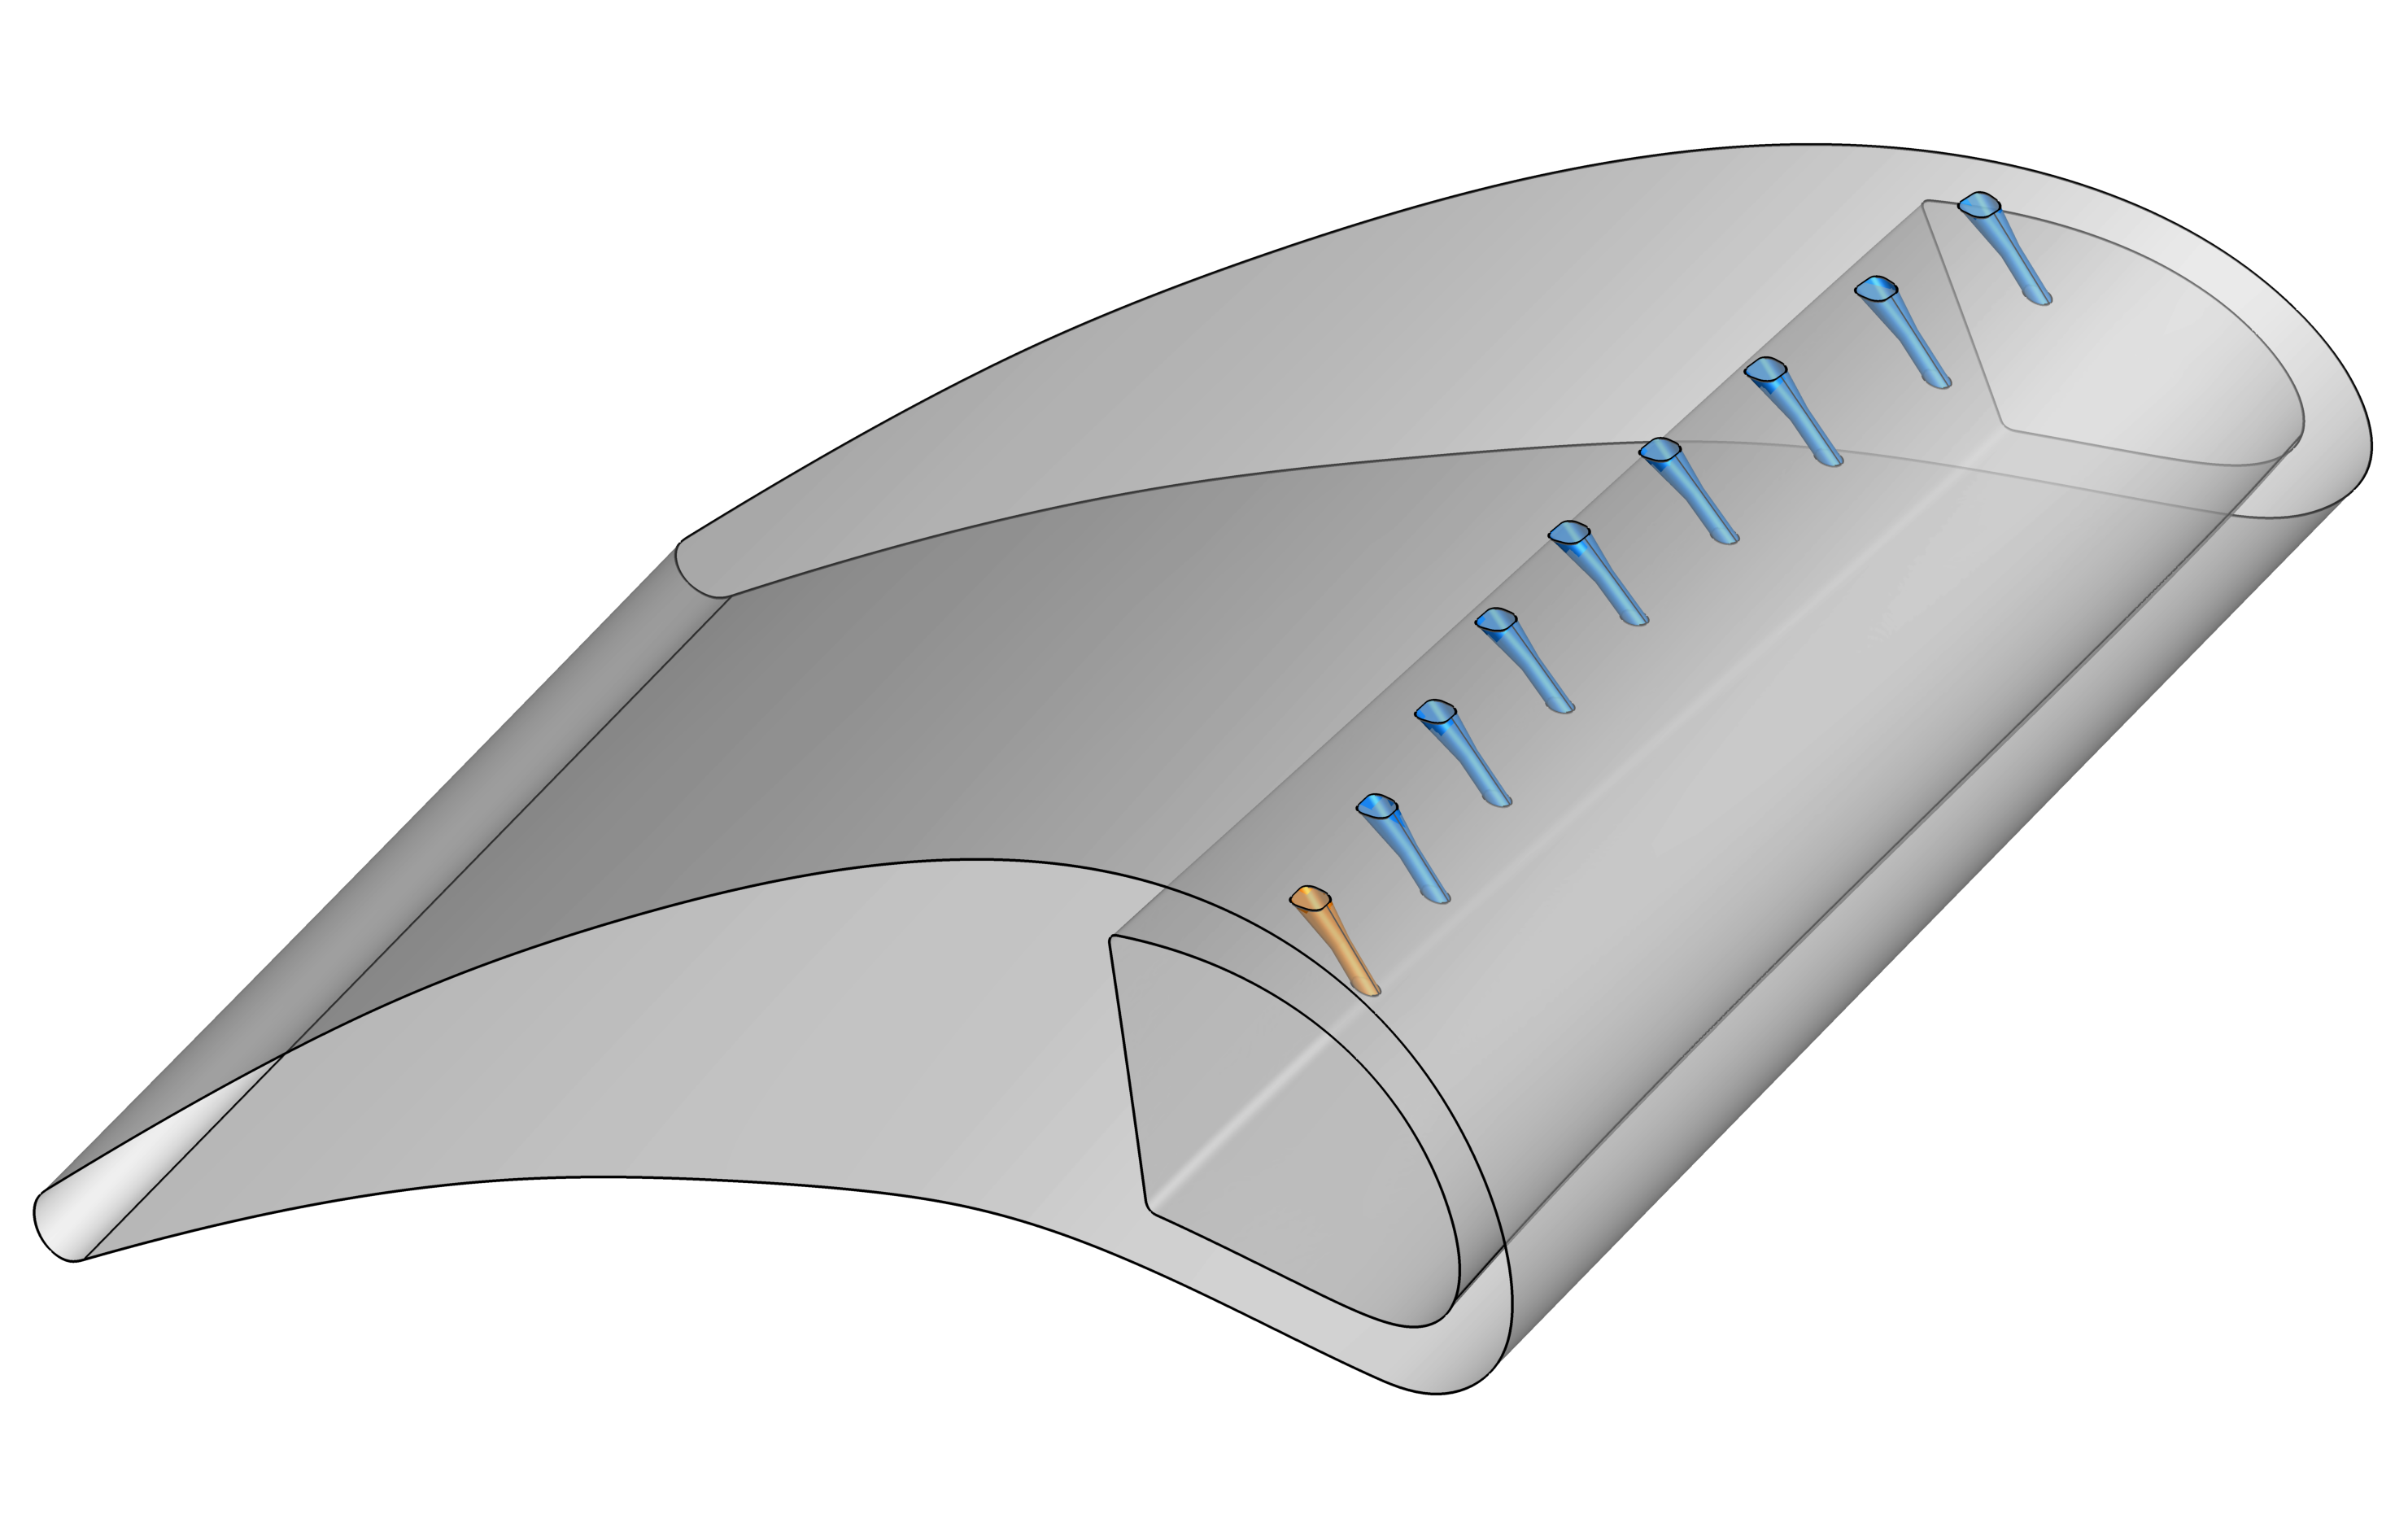
\includegraphics[width=\textwidth]{../tec/holes/22edit.png}
			\caption{Channel with film cooling holes.}
		\end{subfigure}
		\phantom{aaaaaaaaaa}
		\begin{subfigure}{.4\textwidth}
			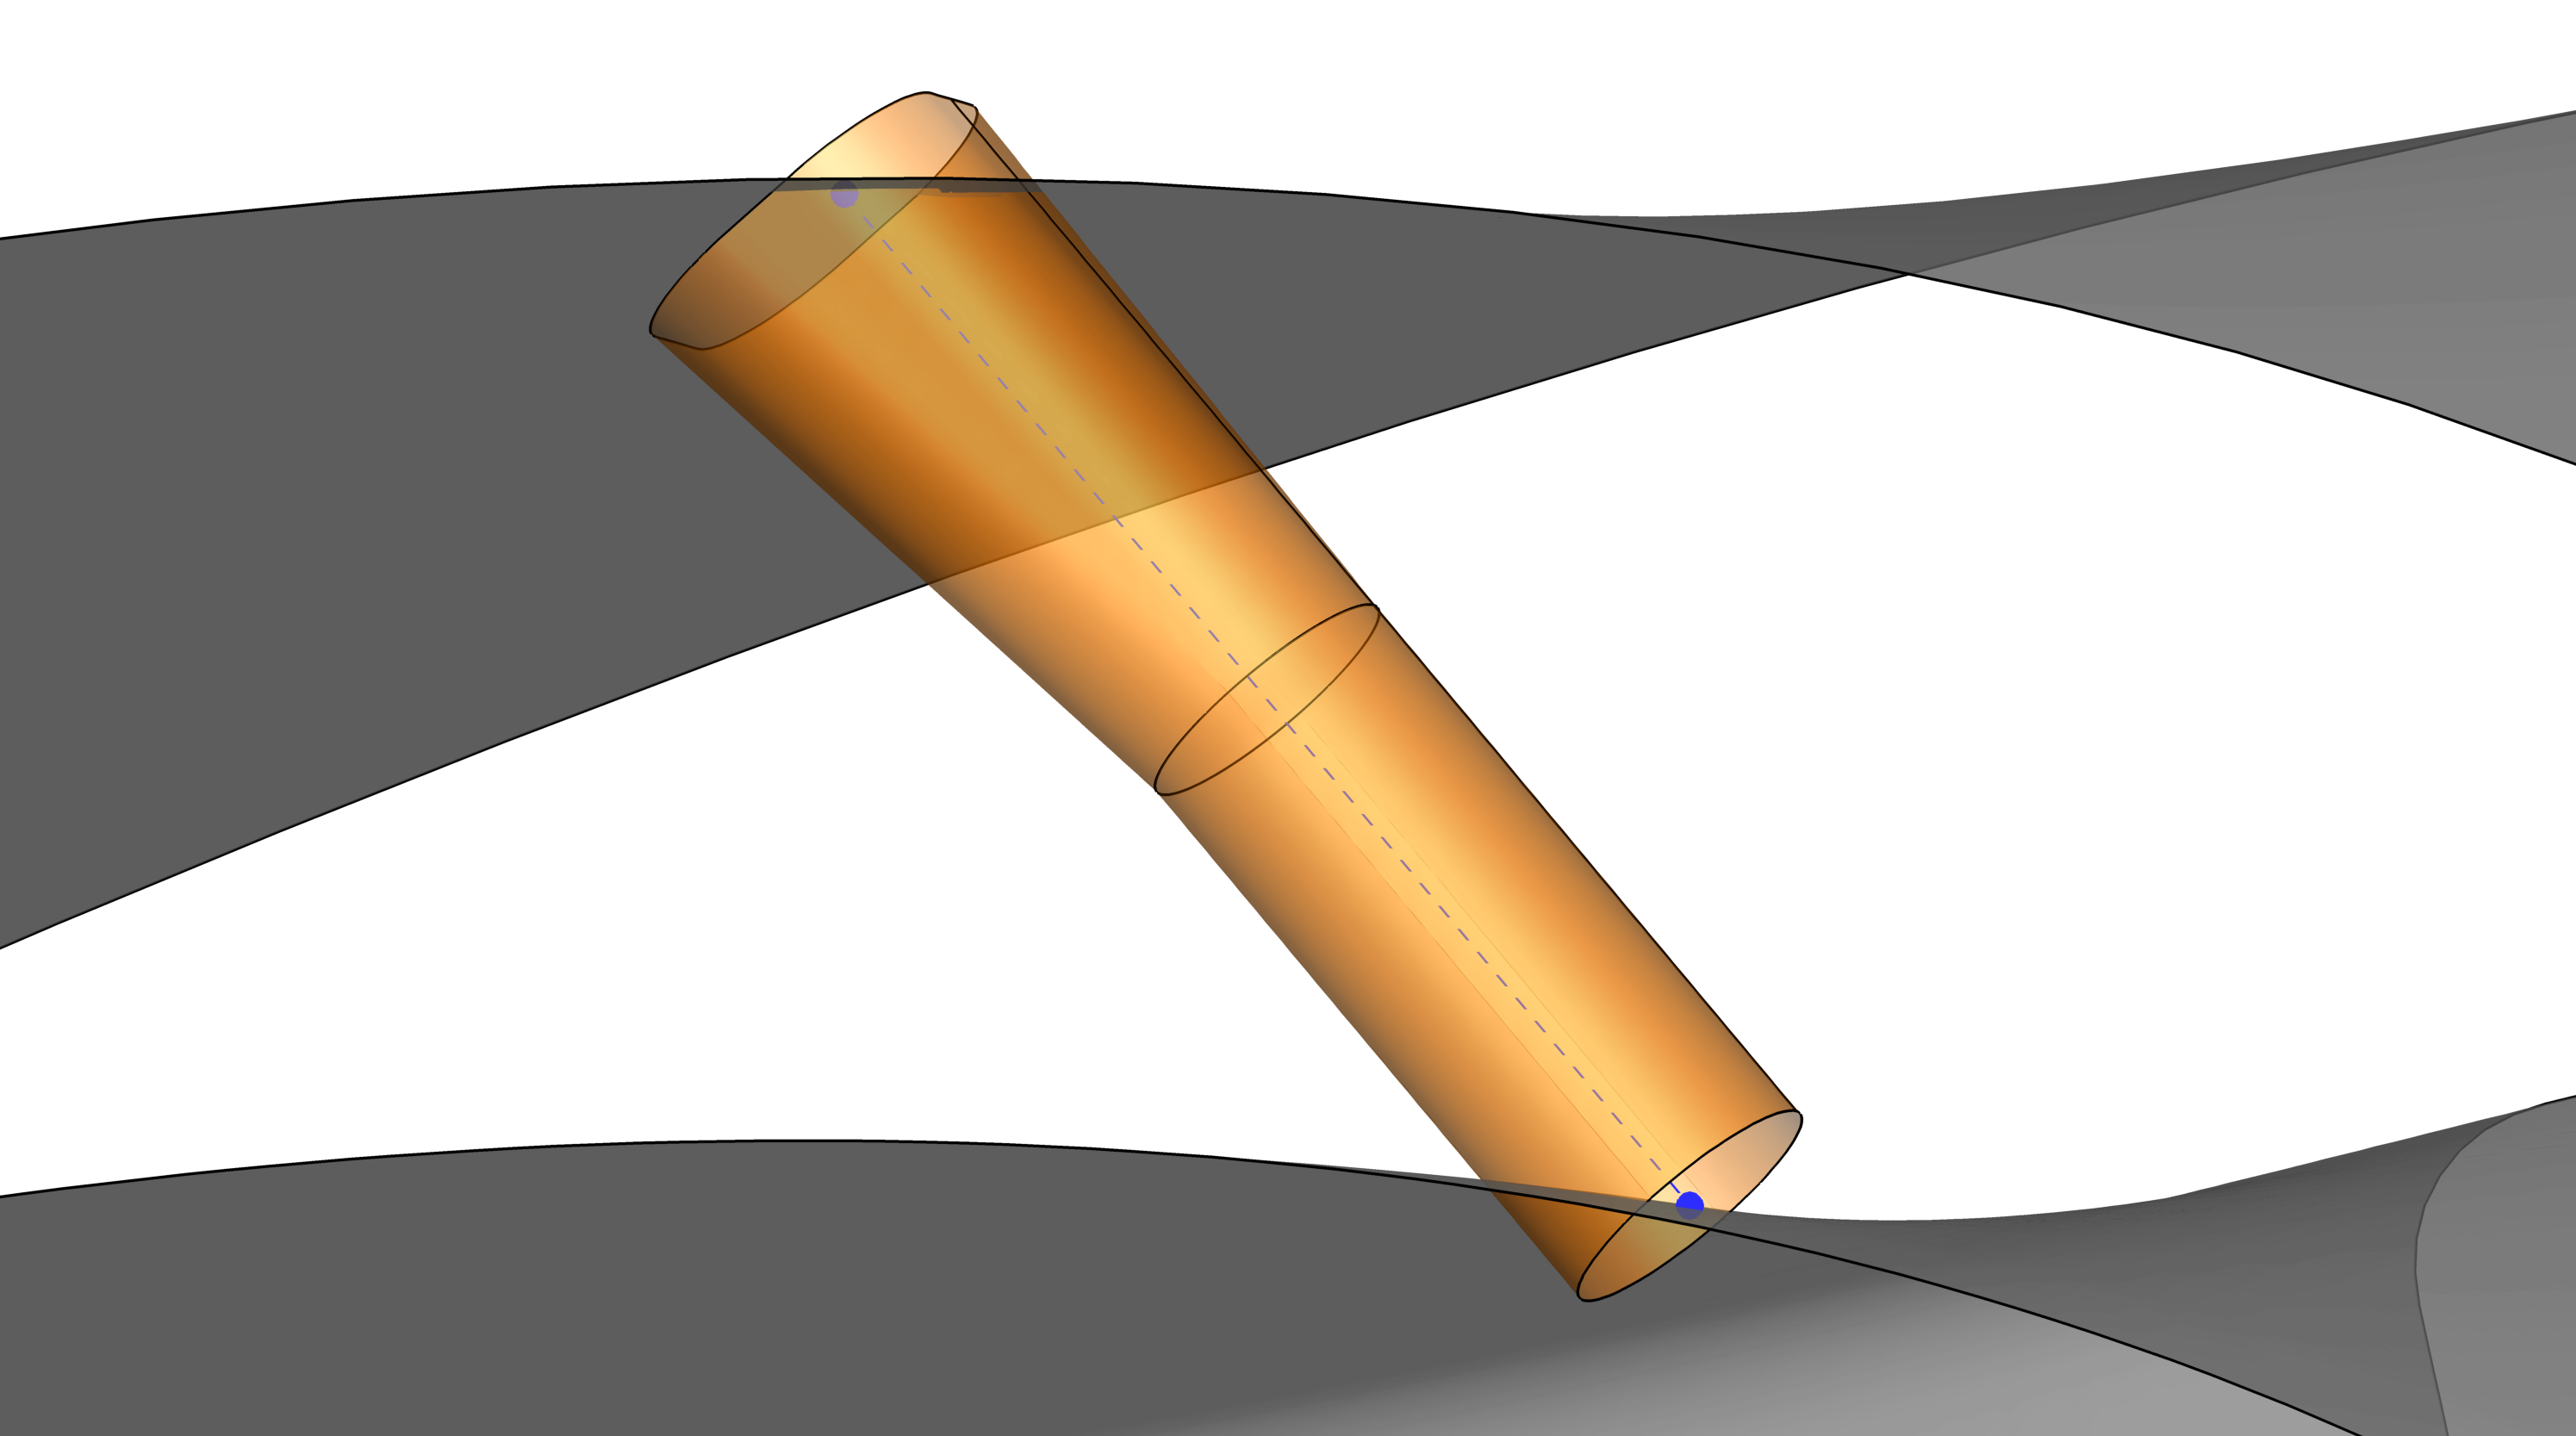
\includegraphics[width=\textwidth]{../tec/holes/20edit.png}
			\caption{Film cooling hole surface $F^{(v_\textrm{transition})}$.}
		\end{subfigure}\\
		\begin{subfigure}{.5\textwidth}
			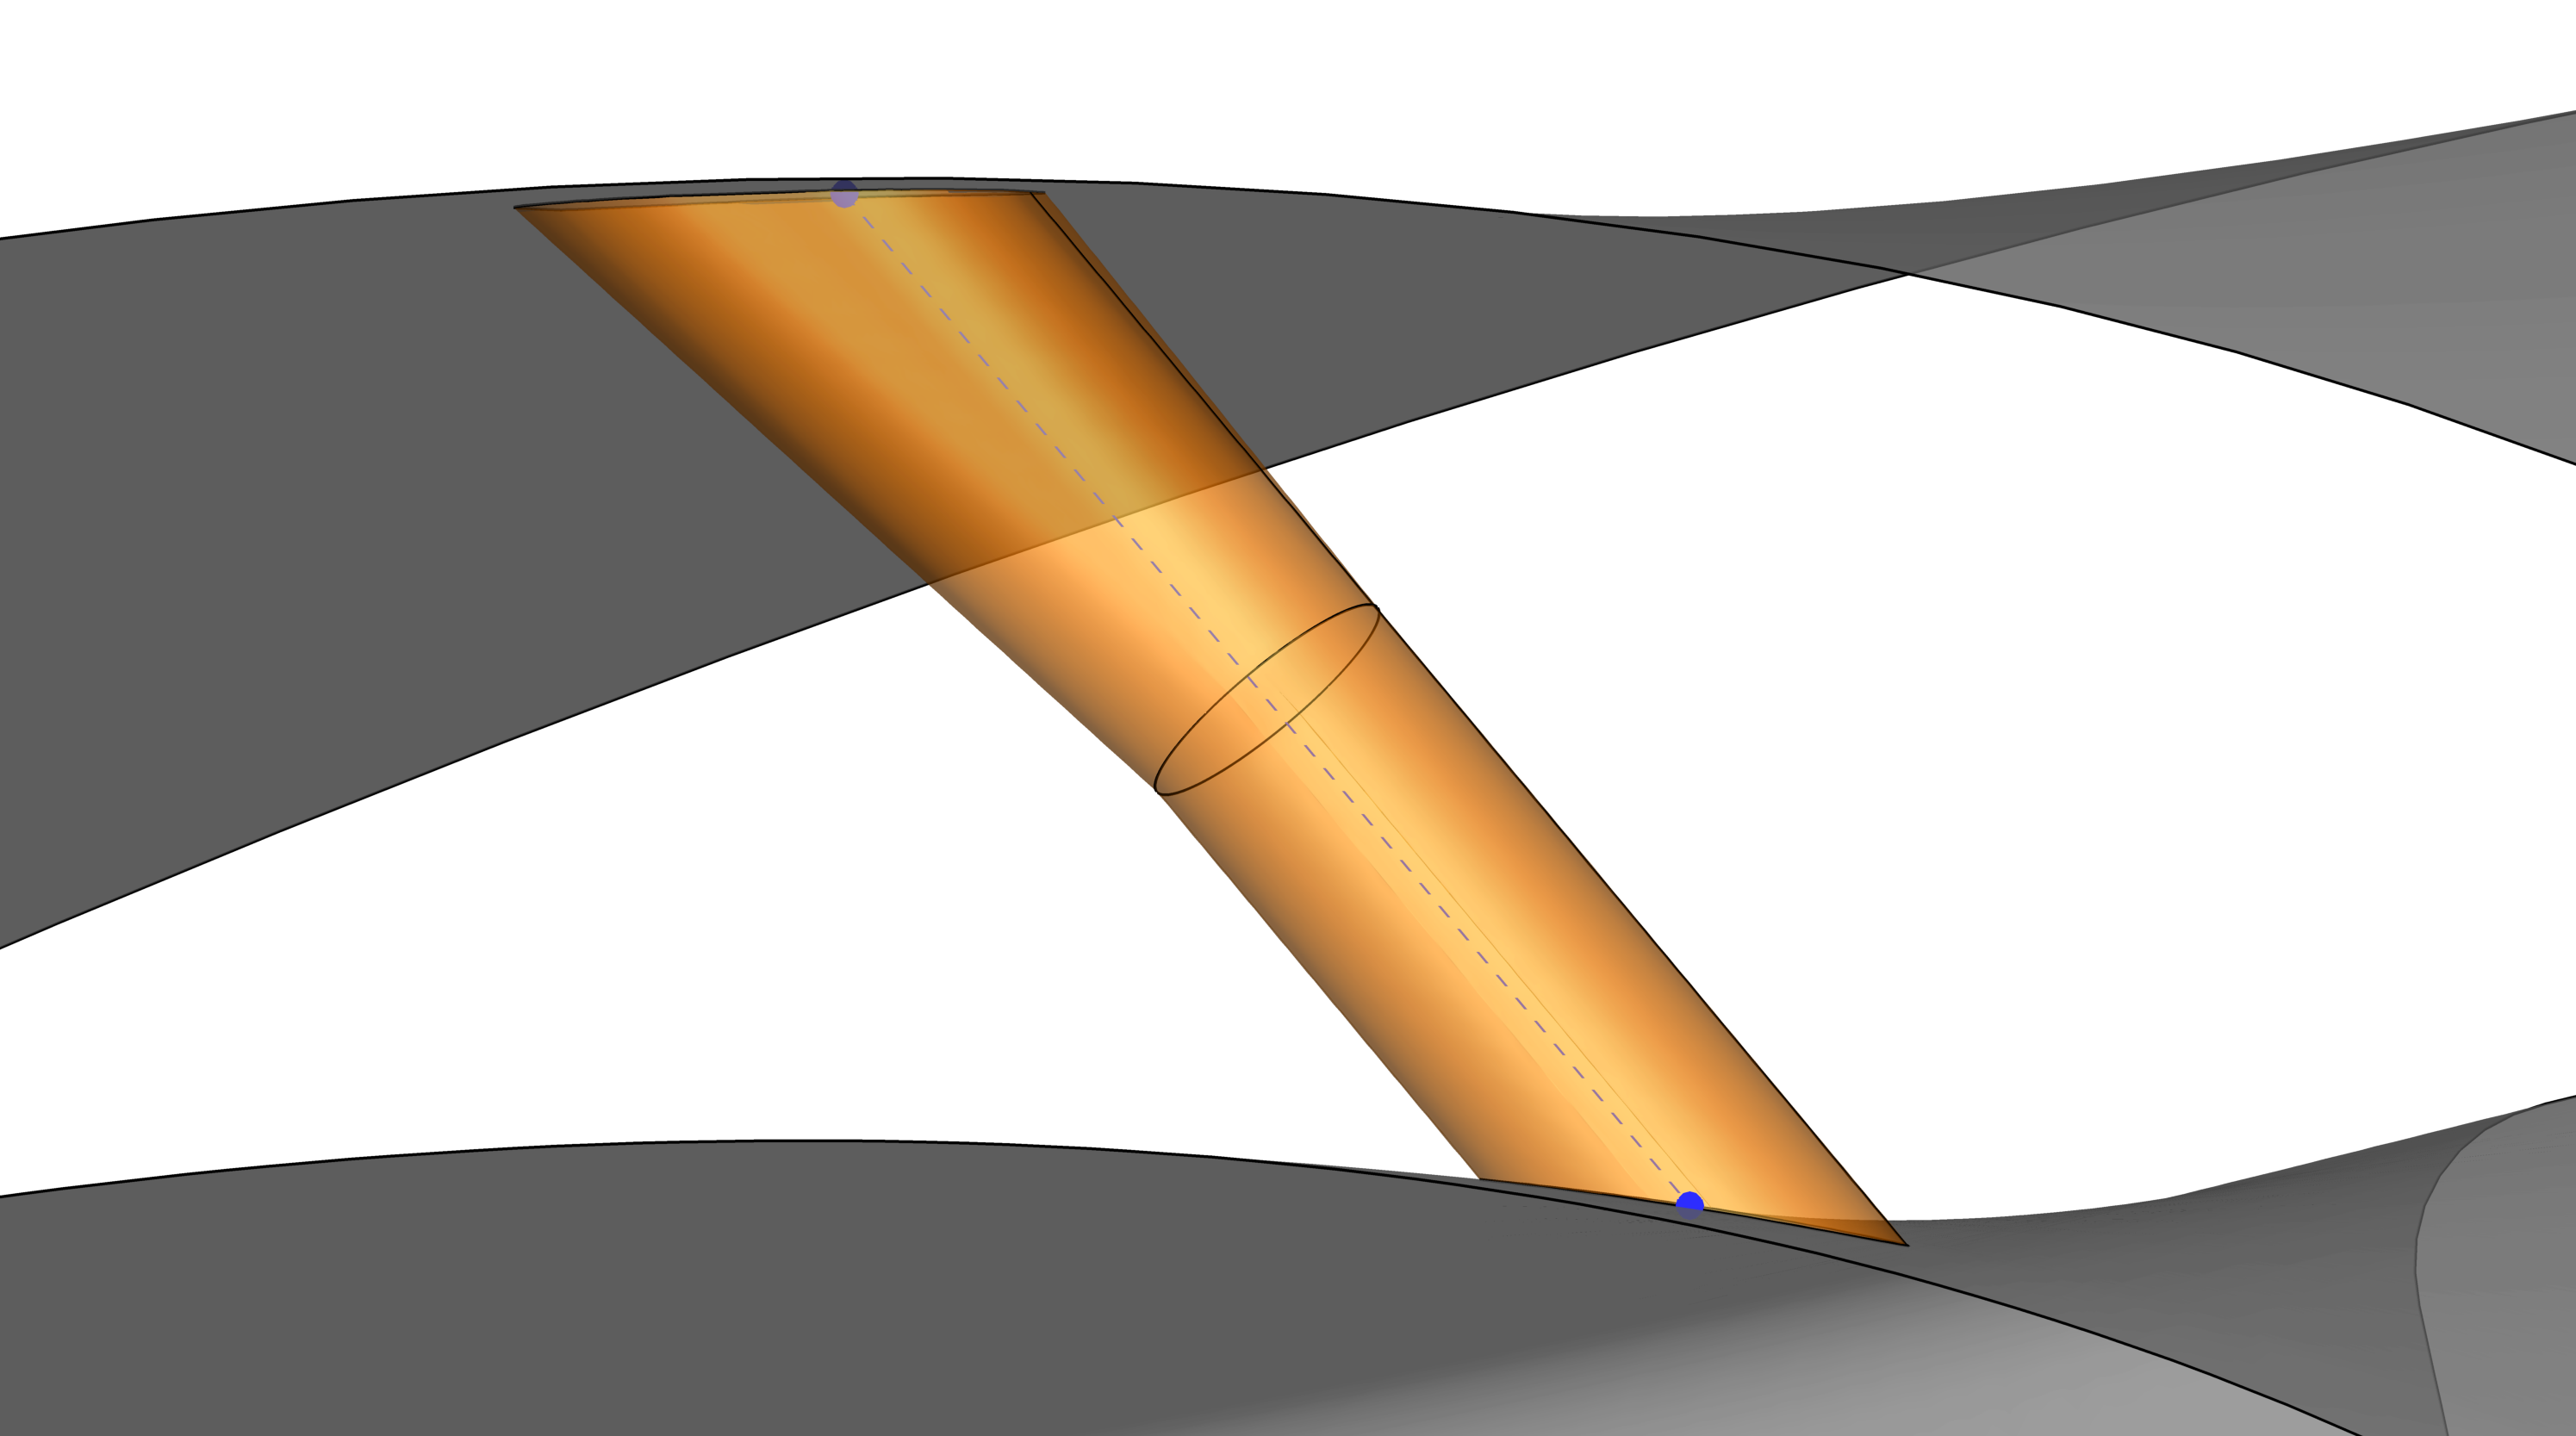
\includegraphics[width=\textwidth]{../tec/holes/21edit.png}
			\caption{Ray intersected film cooling hole surface $\Phi$.}
		\end{subfigure}
		\caption{Intersecting a film cooling hole using ray intersection.}
		\label{fig:filmholeintersection}
	\end{figure}

	Notice that using this process, the start and end points of $P_B$ and $P_C$ are now aligned to the corresponding surfaces $B(u,v)$ and $C(u,v)$, but the two surface boundaries $F^{(v_\textrm{transition})}(u,0)$ and $F^{(v_\textrm{transition})}(u,1)$ do not align with the surfaces $B(u,v)$ and $C(u,v)$, respectively. Notice also that the basic shape of the surface $F^{(v_\textrm{transition})}(u,v)$ has the following property regarding rays:
		$$ F^{(v_\textrm{transition})}([0,1]^2) \subset \bigcup_{v_F \in \{0,1\}}\bigcup_{u_F\in[0,1]} R_{P,Q-P}([0, \infty)), $$
	where $P := F^{(v_\textrm{transition})}(u_F,v_\textrm{transition})$ and $Q := F^{(v_\textrm{transition})}(u_F,v_F)$.
	In other words, the film cooling hole is made up out of line segments or, equivalently, subsets of rays, the support and direction vectors of which we already know.

	This observation gives rise to a solution to our boundary problem. We can use the ray marching algorithm from Section \ref{subsec:raymarching} to find ray intersections of all such $R_{P,Q-P}$ and $B(u,v)$ by setting $v_F = 0$. This yields a delimiting curve $B_d(u)$, which marks one boundary of the film cooling hole and lies completely within $B(u,v)$. By setting $v_F = 1$, we find the ray intersections of all such $R_{P, Q-P}$ and $C(u,v)$, yielding a delimiting curve $C_d(u)$ which marks the other boundary of the film cooling hole and lies completely within $C(u,v)$.

	We are left with three important curves. The blade or vane delimiting curve $B_d(u)$, the transition isocurve $F^{(v_\textrm{transition})}(u,v_\textrm{transition})$ and the channel delimiting curve $C_d(u)$. We can linearly interpolate between these three curves. The intersected film cooling hole surface is then equal to
		$$ \Phi(u,v) = 
				\begin{cases}
					\frac{v_\textrm{transition} - v}{v_\textrm{transition}} \, B_d(u) +
					\frac{v}{v_\textrm{transition}} \, F^{(v_\textrm{transition})}(u,v_\textrm{transition})
					& \textrm{ if } v \leq v_\textrm{transition}, \\

					\\[-0.5em]
					
					\frac{1 - v}{1 - v_\textrm{transition}} \, F^{(v_\textrm{transition})}(u,v_\textrm{transition}) + 
					\frac{v - v_\textrm{transition}}{1 - v_\textrm{transition}} \, C_d(u)		
					& \textrm{ else.}

				\end{cases}
		 $$

	Using this procedure, we can efficiently create multiple film cooling holes. In CoolingGen, a distribution function is used to create a row of multiple film cooling holes at once that share the same direction $D$, radius $r$ and shape parameters $b, d$, but differ in position. This distribution function takes the number of holes $H \in \mathbb{N}$, a parameter $u_B \in [0,1]$ and an interval $[v_L, v_U] \subset [0,1]$ as an input and distributes $H$ film cooling holes on $B(u_B, [v_L, v_U])$. Multiple of these rows are usually specified.

\section{Impingement Inserts}
	To construct an impingement insert, we use two surfaces to model the outer and the inner surface of the sheet that reside within the channel, respectively. The holes in this sheet are represented by cylindrical surfaces. Notice that the creation of impingement inserts is not compatible with the creation of channels with turns.

	\begin{figure}[H]
		\centering
		\begin{subfigure}{.37\textwidth}
			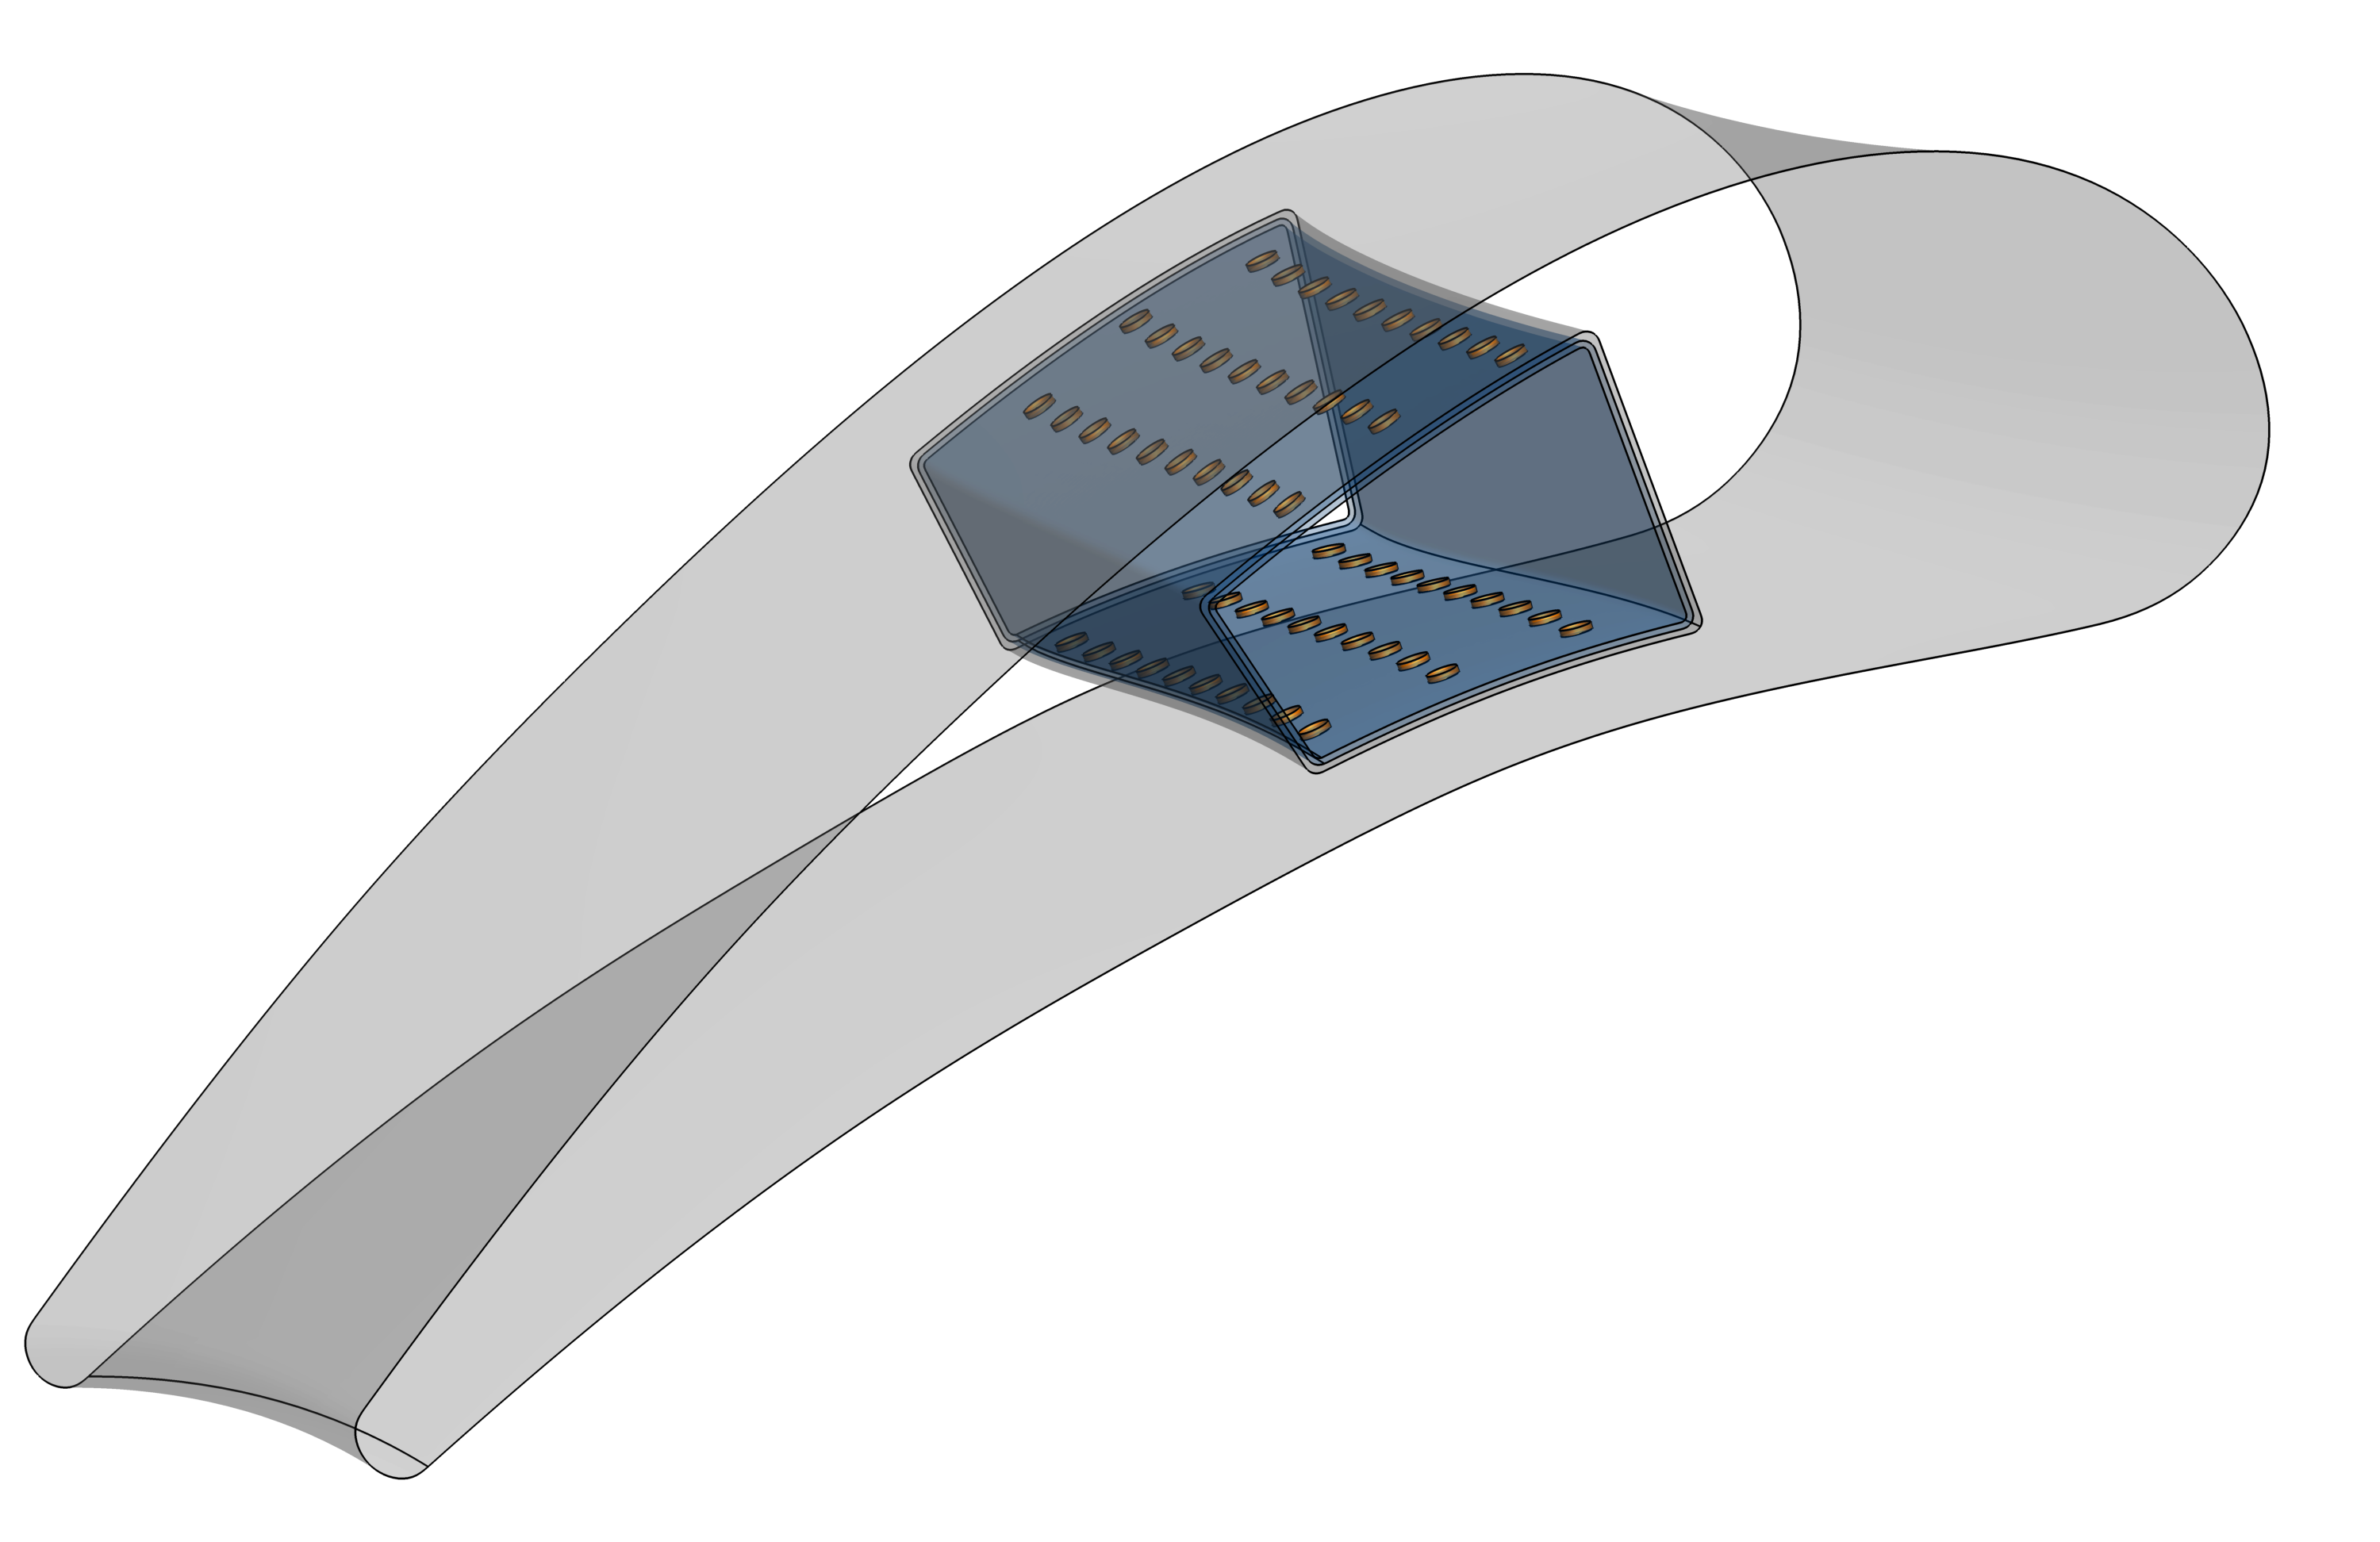
\includegraphics[width=\textwidth]{../tec/impingement/00.png}
			\caption{Radial view with channel and blade.}
		\end{subfigure}
		\begin{subfigure}{.37\textwidth}
			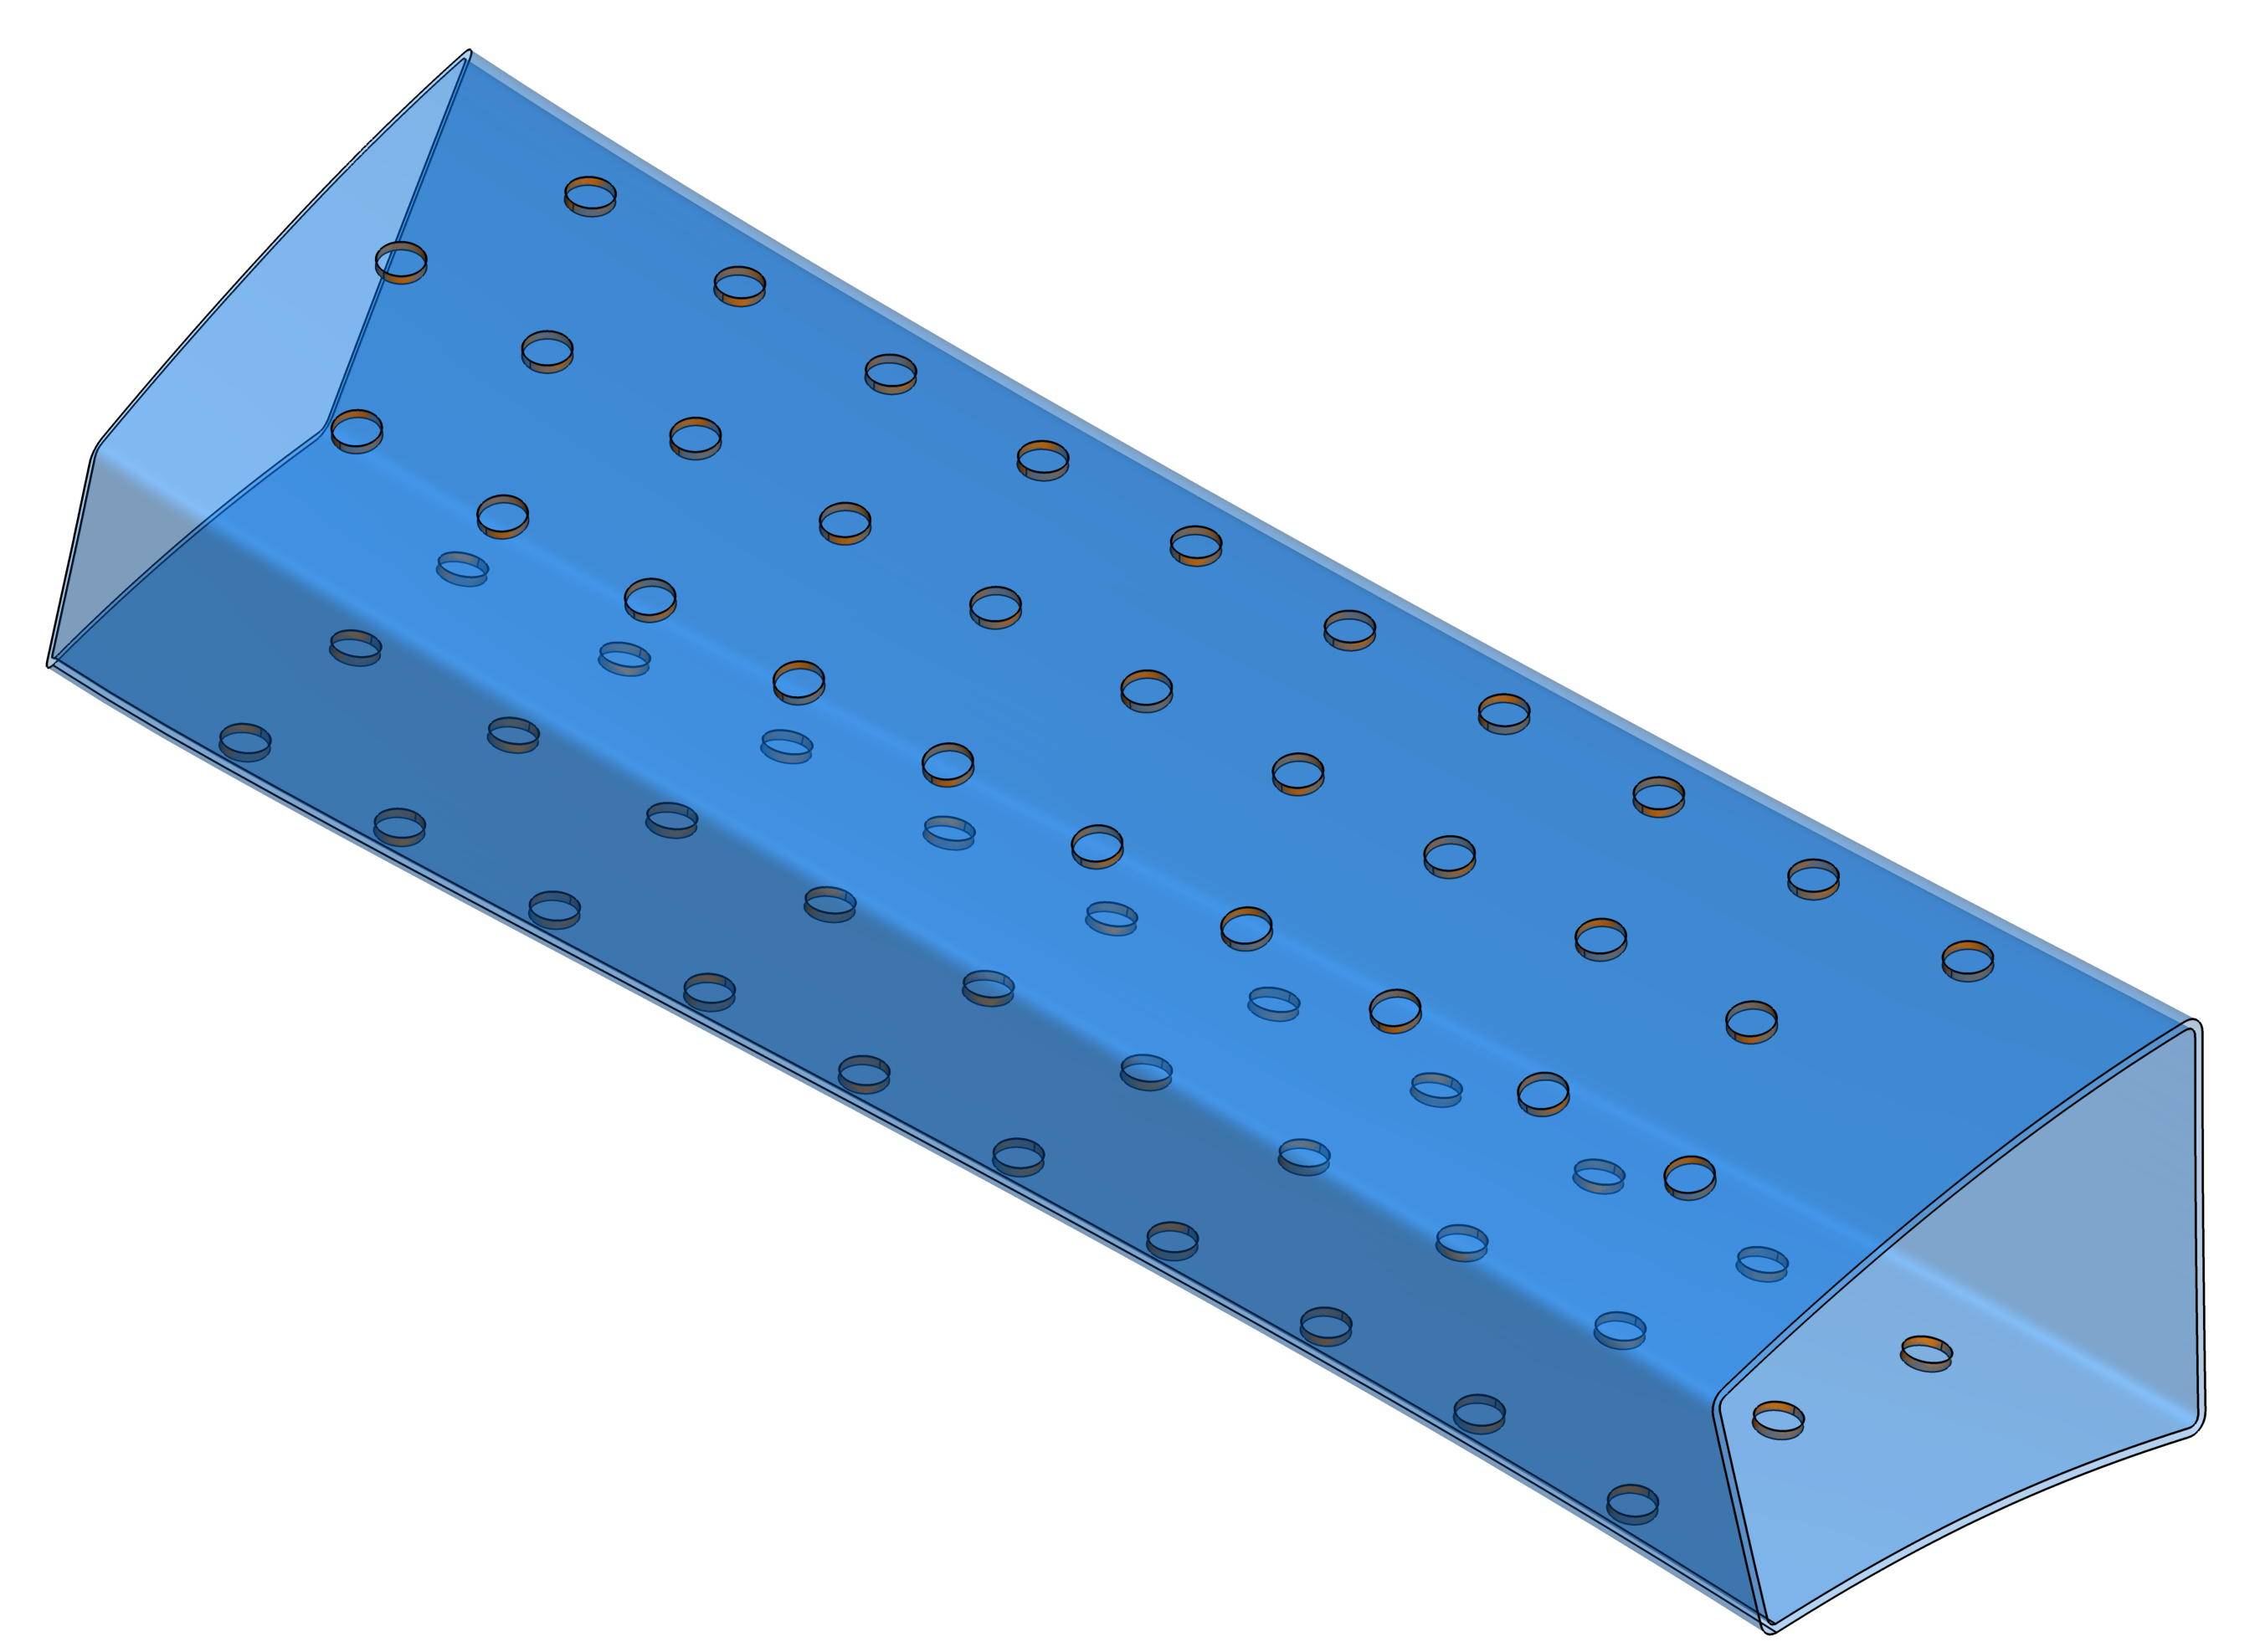
\includegraphics[width=\textwidth]{../tec/impingement/02.png}
			\caption{Suction-sided view.}
		\end{subfigure}\\
		\begin{subfigure}{.5\textwidth}
			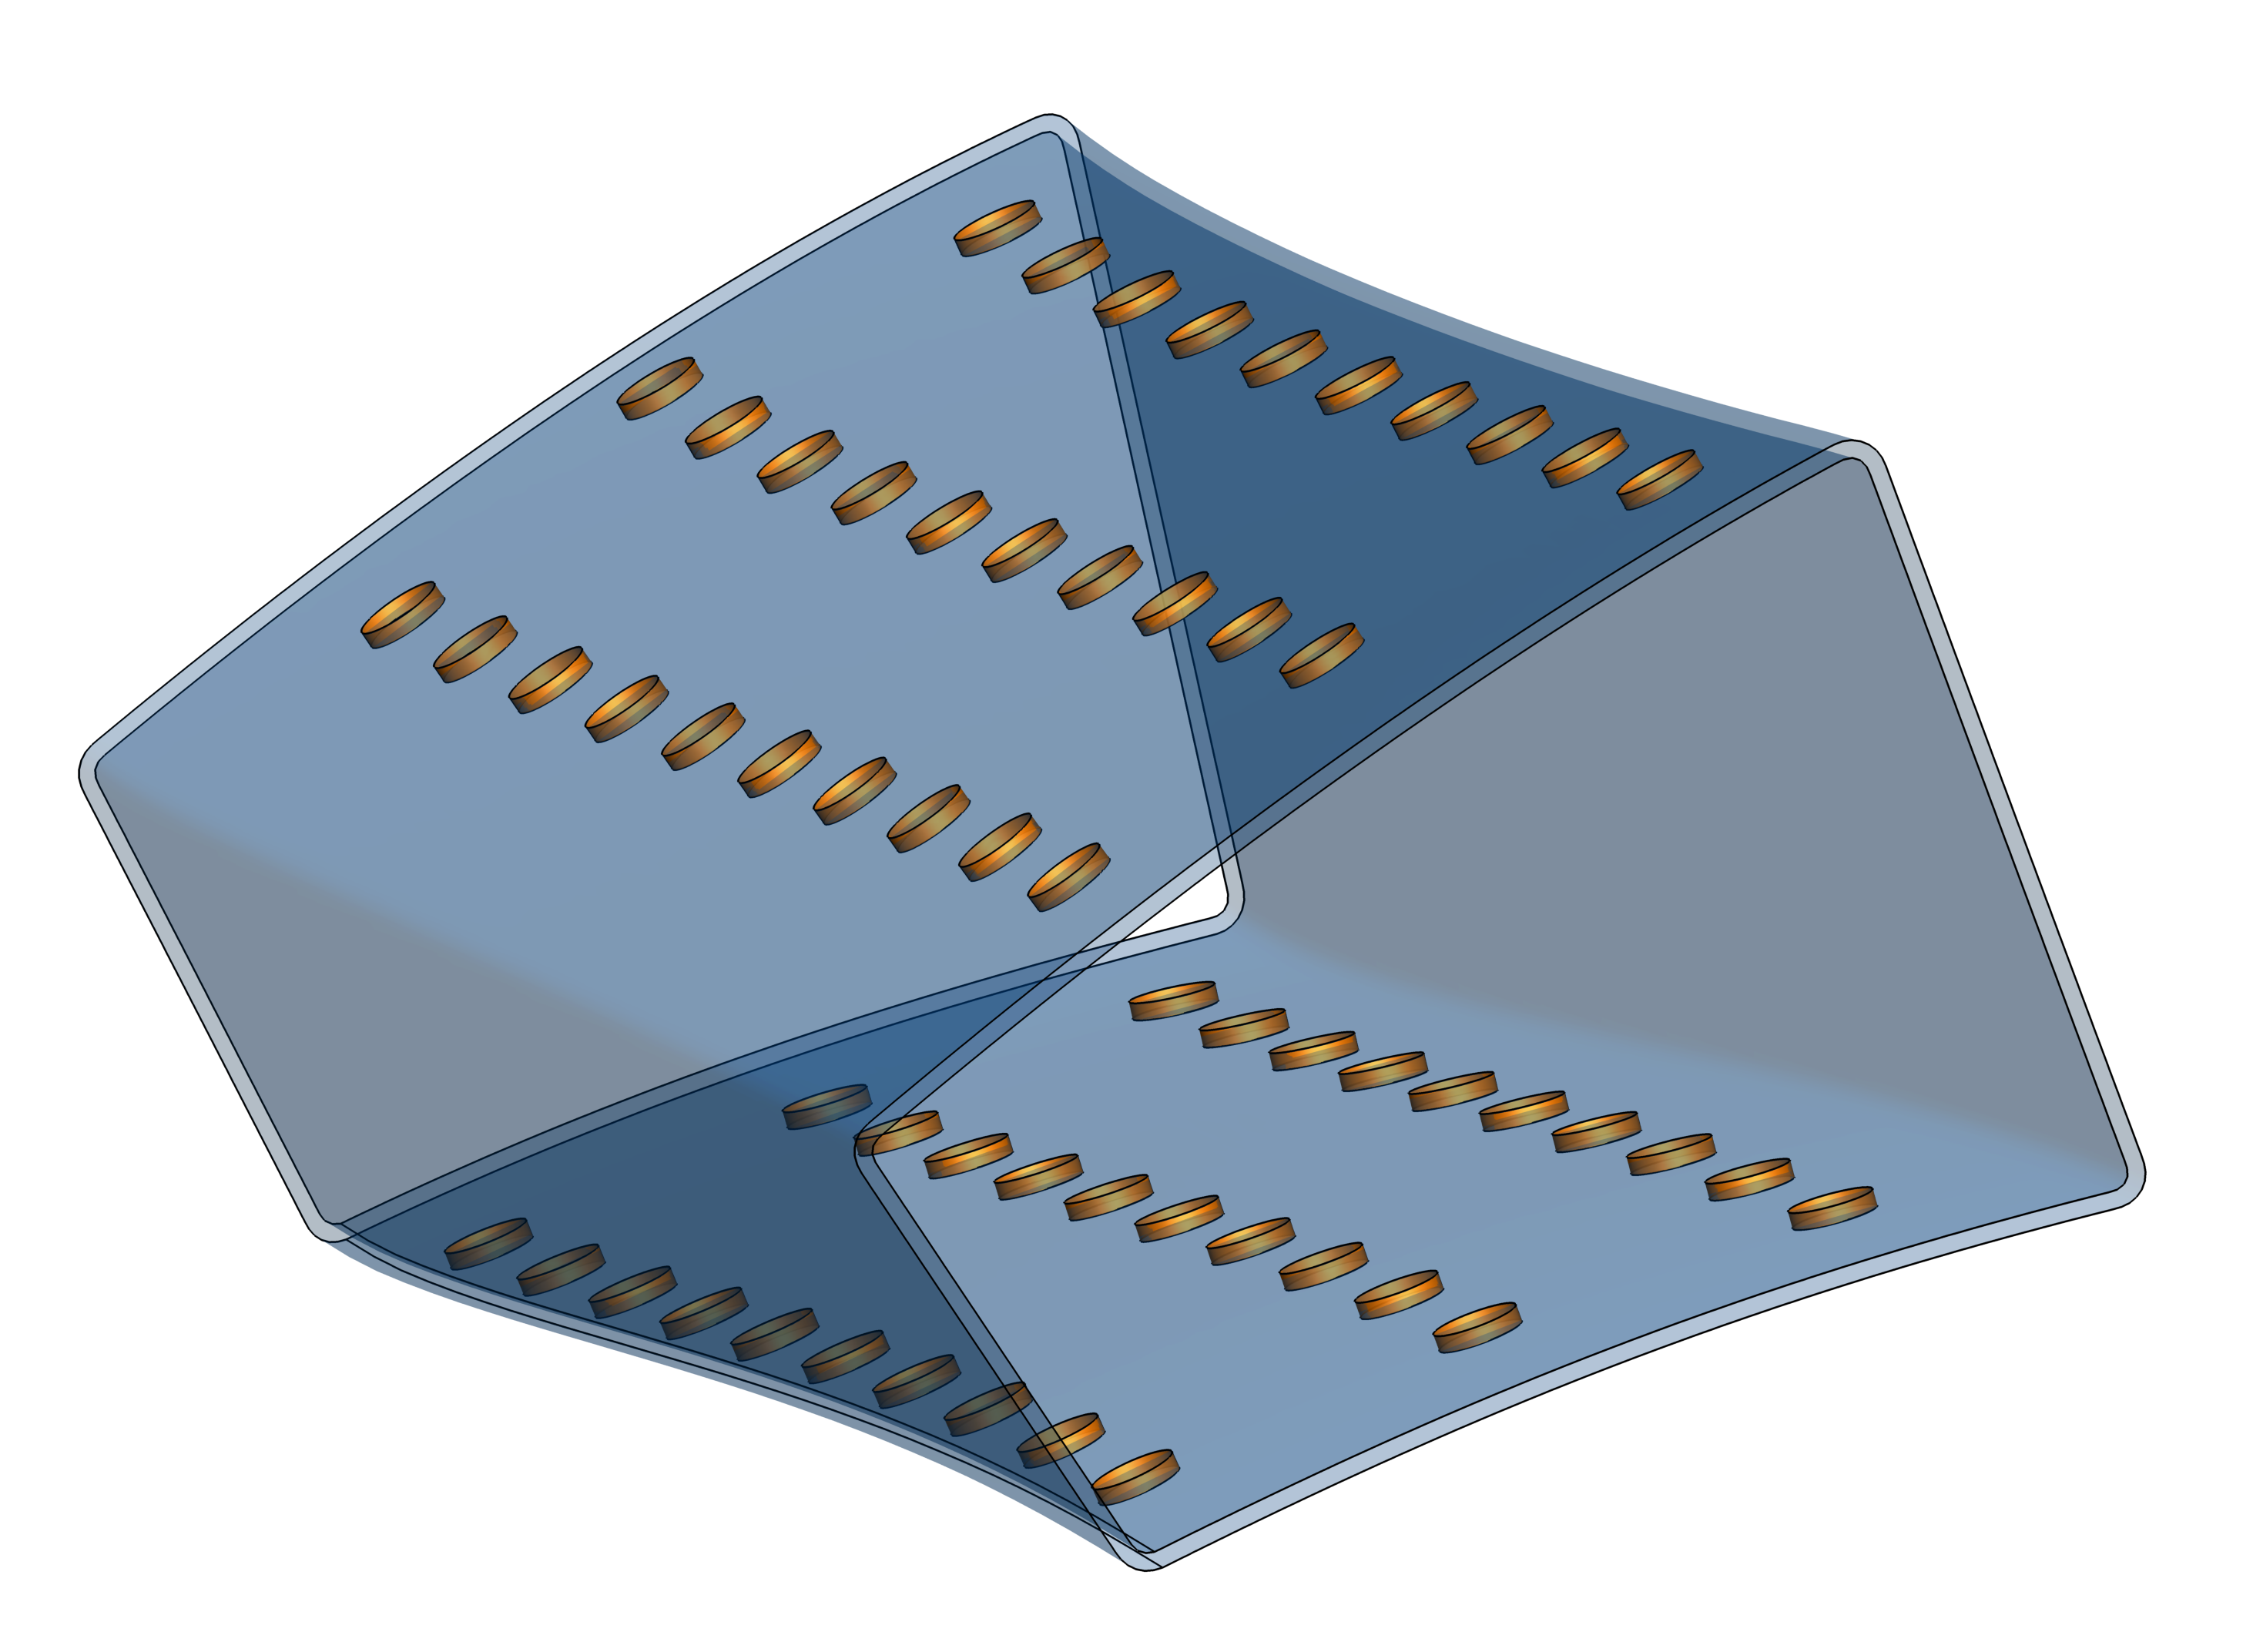
\includegraphics[width=\textwidth]{../tec/impingement/01.png}
			\caption{Radial view.}
		\end{subfigure}
		\caption{An impingement insert with staggered holes on the suction side and aligned holes on the pressure side.}
		\label{fig:impingementinsert}
	\end{figure}

	The creation of the inner and outer surfaces relies on the same principles as the creation of chambers, which was discussed in Section \ref{sec:chambers}. Since we already calculated the $(m, r\theta)$ profiles of the chambers, we only need to offset, trim, add fillets and use skinning to make these surfaces. For each impingement insert, an inner distance $i > 0$, outer distance $o > 0$ and a thickness $d > 0$ is specified.

	The profile partitions that run parallel to the blade or vane are offset by $o$, whereas the profile partitions that lie between chambers are offset by $i$. The new profile partitions are trimmed and fillets are added. This yields the outer impingement insert profile. The outer impingement insert profiles are then offset by $d$ to calculate the inner impingement insert profiles. After using surface skinning, we are left with two surfaces that represent the impingement insert, an example of which can be seen in Figure \ref{fig:impingementinsert}.
	
	\begin{figure}[H]
		\centering
		\begin{subfigure}{.25\textwidth}
			\includesvg[width=\textwidth]{../python/alignedstaggered_aligned}
			\caption{Aligned pattern.}
		\end{subfigure}
		\phantom{aaaaaaaaaaa}
		\begin{subfigure}{.25\textwidth}
			\includesvg[width=\textwidth]{../python/alignedstaggered_staggered}
			\caption{Staggered pattern.}
		\end{subfigure}
		\caption{Aligned and staggered pattern of impingement insert holes.}
		\label{fig:alignedstaggered}
	\end{figure}

	Using the methods from \ref{sec:filmcooling}, we can construct cylindrical holes between the outer and inner surface of the impingement insert. Instead of using a distribution function for positioning, we instead specify two intervals $[u_L, u_U]$ and $[v_L, v_U]$ on the outer impingement insert surface and the number of rows $N$ and columns $M$ of film cooling holes per array, to place (up to) $NM$ holes between the outer and inner impingement insert surface, inside the specified intervals. We also specify the type of hole distribution, which can be either aligned or staggered. These two types can be seen in Figure \ref{fig:alignedstaggered} and Figure \ref{fig:impingementinsert}.

\section{Ejection Slots}\label{sec:slots}
	Ejection slots transport the coolant from the inside of the trailing edge channel to the pressure side of the blade or vane. A slot is partially defined by two delimiting surfaces, the inlet surface $I(u,v)$ and the outlet surface $O(u,v)$ for $u,v \in [0,1]$. The inlet surface $I(u,v)$ is a subsurface of the channel surface $C(u,v)$ that lies closest to the trailing edge. The outlet surface $O(u,v)$ is a subsurface of the blade or vane surface $B(u,v)$.

	\begin{figure}[H]
		\centering
		\begin{subfigure}{.45\textwidth}
			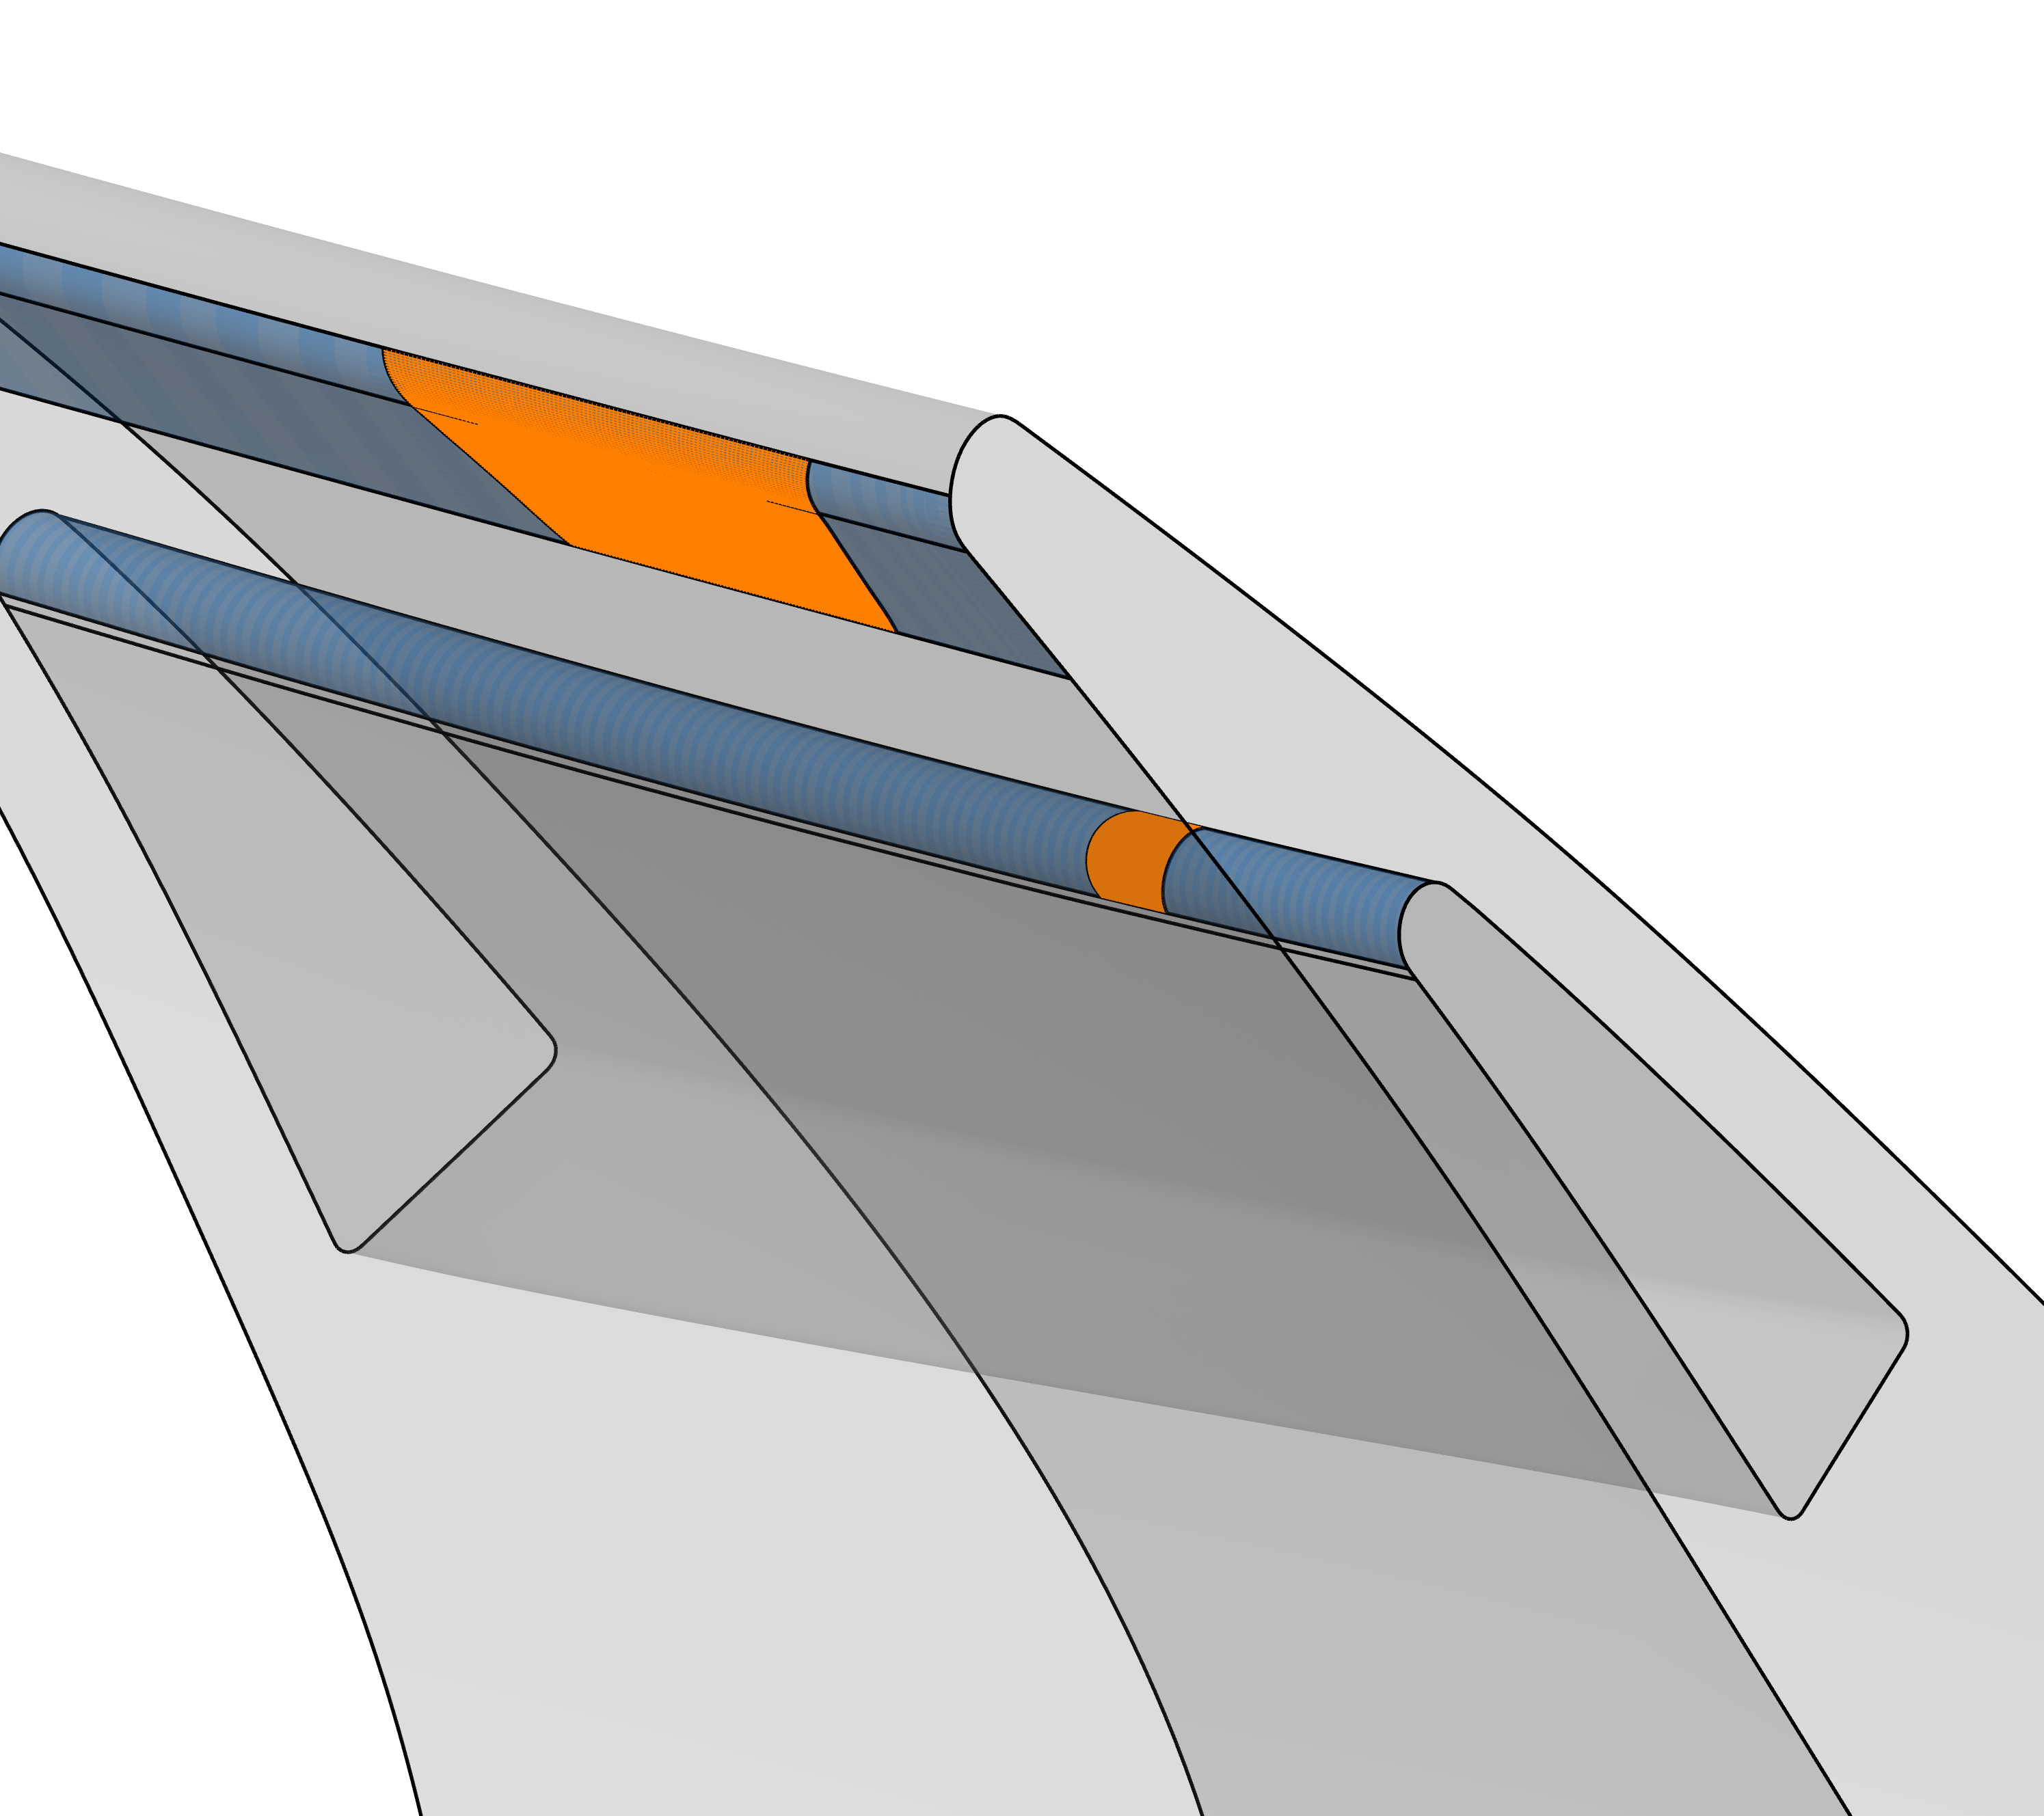
\includegraphics[width=\textwidth]{../tec/slots/14.png}
		\end{subfigure}
		\begin{subfigure}{.45\textwidth}
			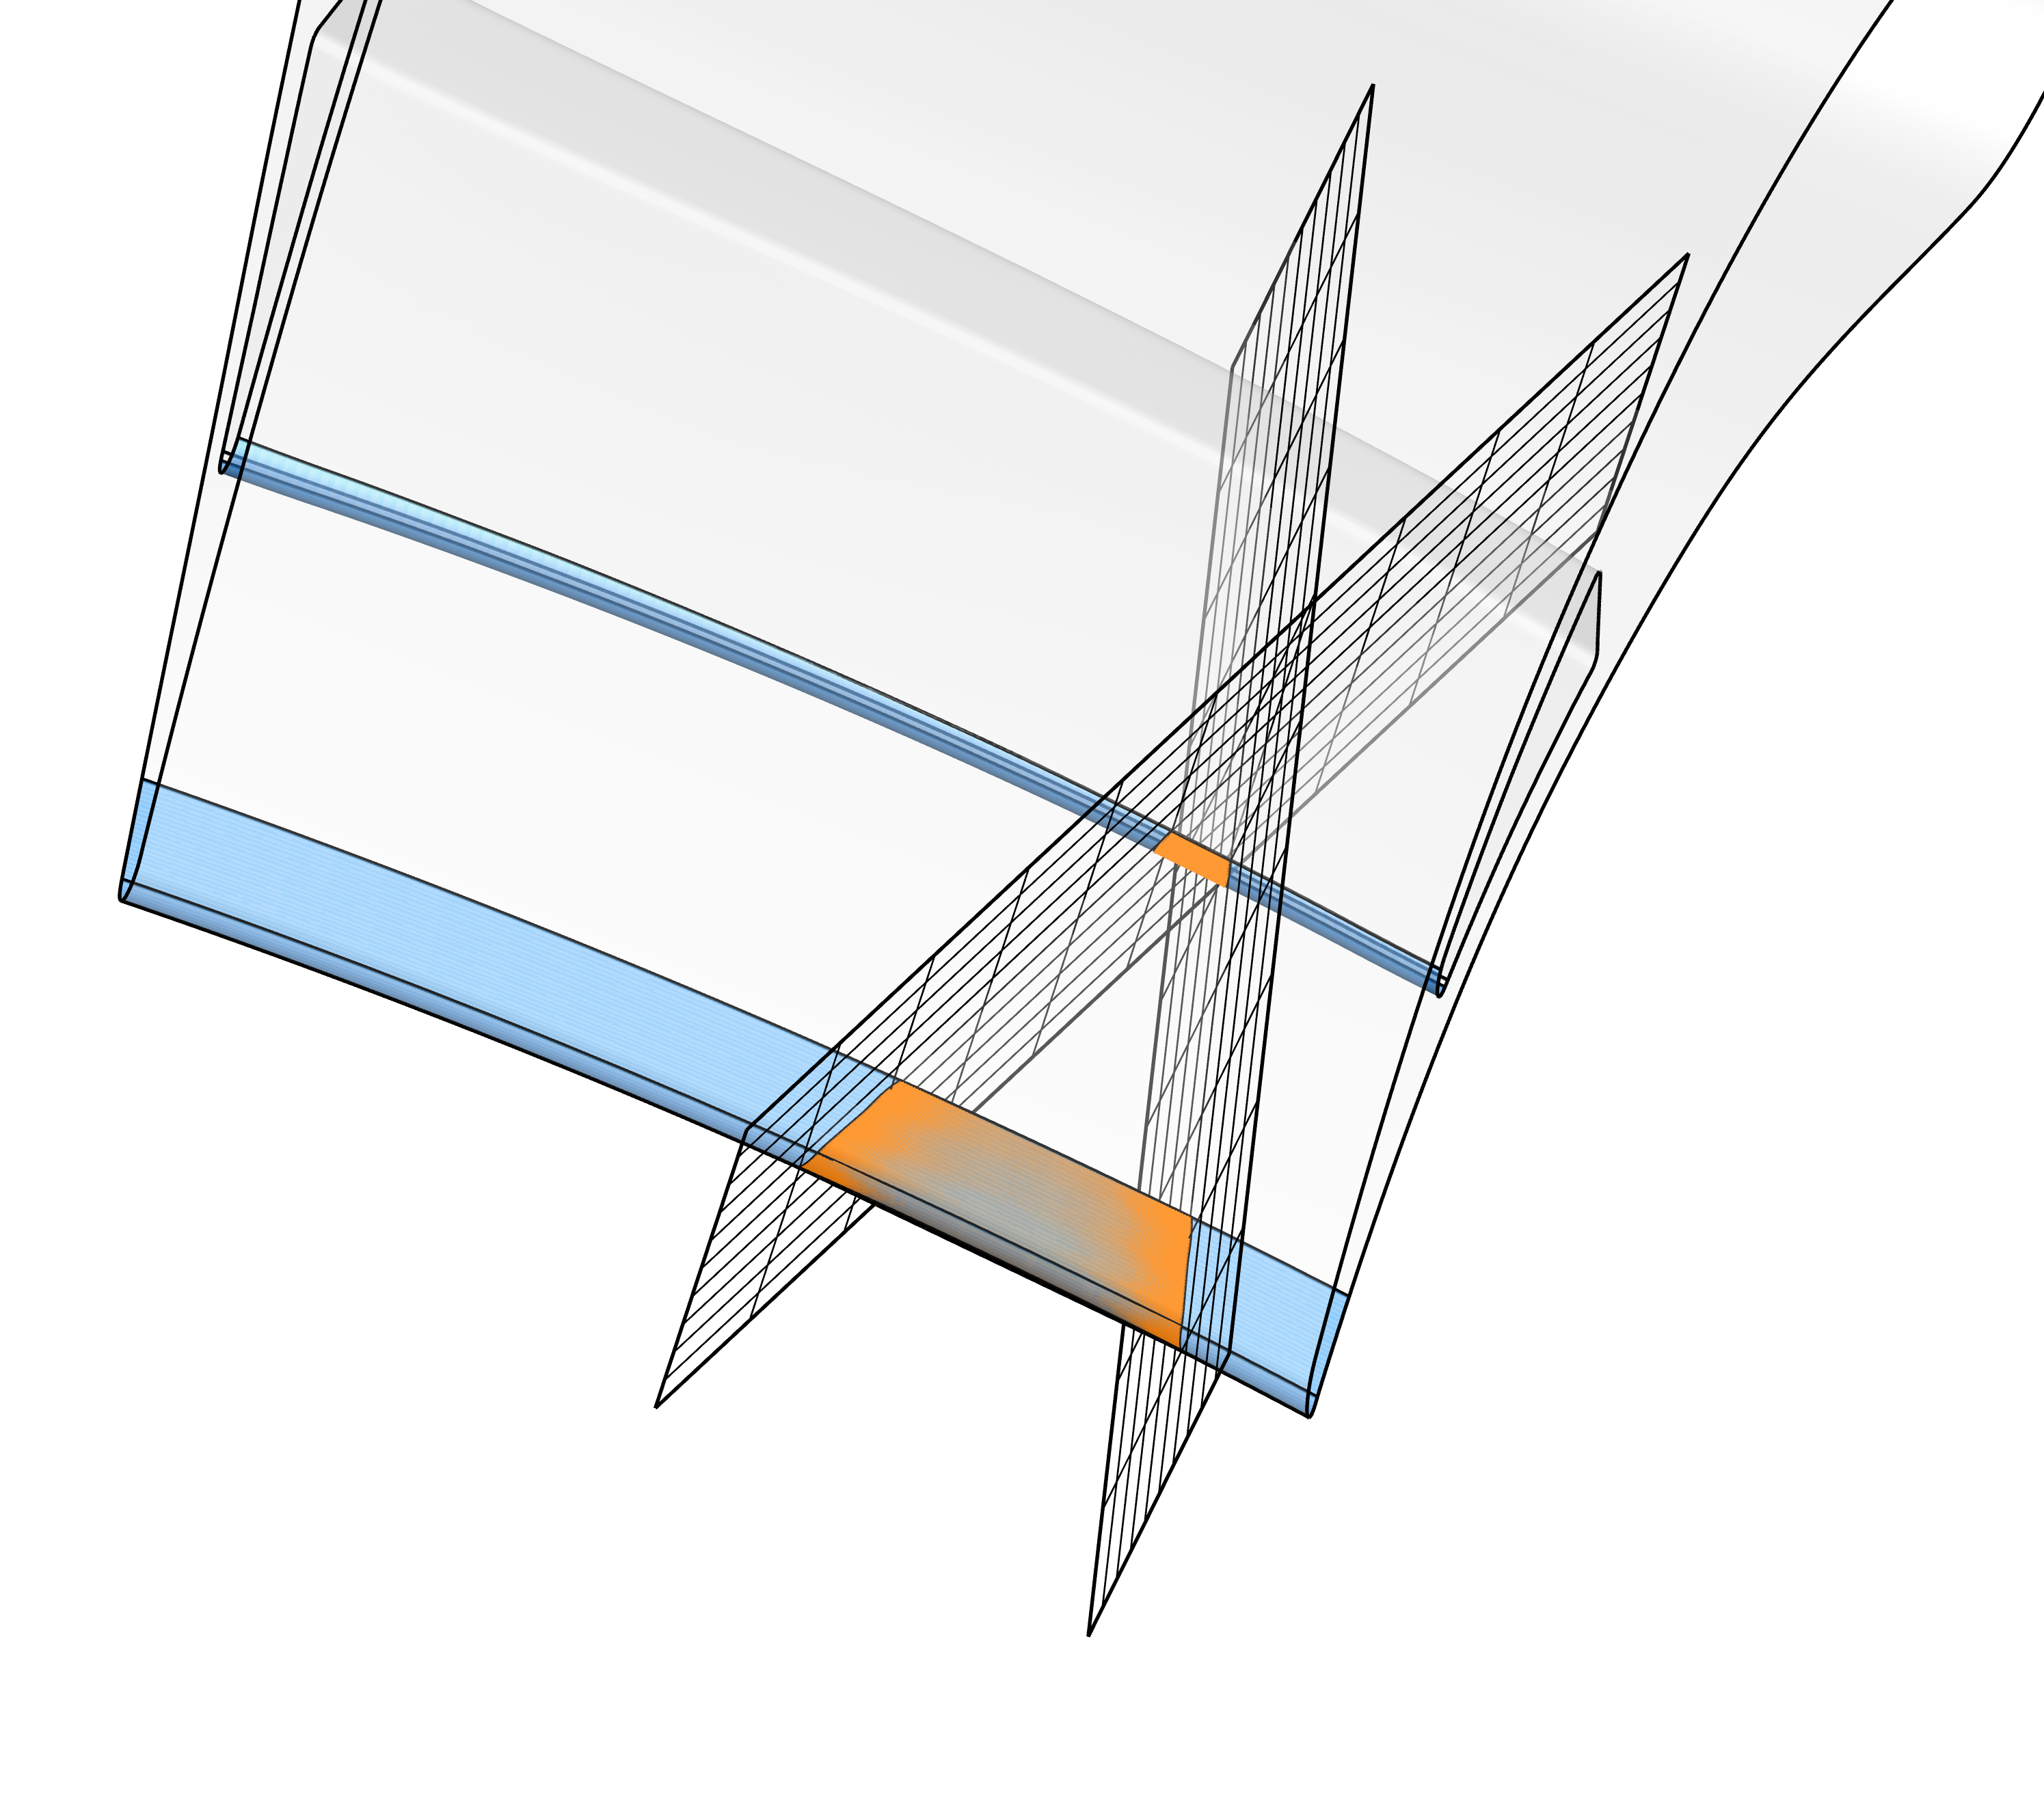
\includegraphics[width=\textwidth]{../tec/slots/15.png}
		\end{subfigure}
		\caption{The inlet surface $I(u,v)$ on the trailing edge channel $C(u,v)$ and the outlet surface $O(u,v)$ on the blade $B(u,v)$ are calculated using plane-surface intersection.}
		\label{fig:slot_plane_intersection}
	\end{figure}

	Given the input lower bounds $u_B^L$ and $u_C^L$ and the input upper bounds $u_B^H$ and $u_C^H$ of $B(u,v)$ and $C(u,v)$, respectively, we can find the subsurfaces
		$$ B\domrestr_{u \in [u_B^L, u_B^H]}(u,v) \quad\text{and}\quad C\domrestr_{u \in [u_C^L, u_C^H]}(u,v),$$
	of $B(u,v)$ and $C(u,v)$, which are represented by the blue surfaces in Figure \ref{fig:slot_plane_intersection}.
	Furthermore, the input for the inlet surface $I(u,v)$ requires a lower bound $v_C^L$ and an upper bound $v_C^H$ of $C(u,v)$. Additionally, two angles $\omega_L$ and $\omega_H$ are specified in relation to the trailing edge of $C(u,v)$. Given this data, we can construct the planes
		$$ P_{C(u_C^L,v_C^L), D_L} \quad\text{and}\quad P_{C(u_C^L, v_C^H), D_H},$$
	where normal vector $D_L$ is given by rotating the vector $C(u_C^L, v_C^H)-C(u_C^L, v_C^L)$ by $\omega_L$ around the vector $C(u_C^H, v_C^L) - C(u_C^L, v_C^L)$. The normal vector $D_H$ is given by rotating the vector $C(u_C^H, v_C^H)-C(u_C^H, v_C^L)$ by $\omega_L$ around the vector $C(u_C^H, v_C^H) - C(u_C^L, v_C^H)$. In this section, the figures show two especially large values for the angles $\omega_L$ and $\omega_H$ to better demonstrate the underlying geometric methods.

	Given the input lower bounds $u_B^L$ and $u_C^L$ and the input upper bounds $u_B^H$ and $u_C^H$ of $B(u,v)$ and $C(u,v)$, respectively, we can find all intersections of the aforementioned planes and subsurfaces using the methods from \ref{sec:surfaceplaneintersection}. This intersection procedure yields two intersection curves per subsurface. We trim the subsurfaces at the intersection curves to find $I(u,v)$ and $O(u,v)$. A representation of $I(u,v)$ and $O(u,v)$ is represented in orange in Figure \ref{fig:slot_plane_intersection}.

	\begin{figure}[H]
		\centering
		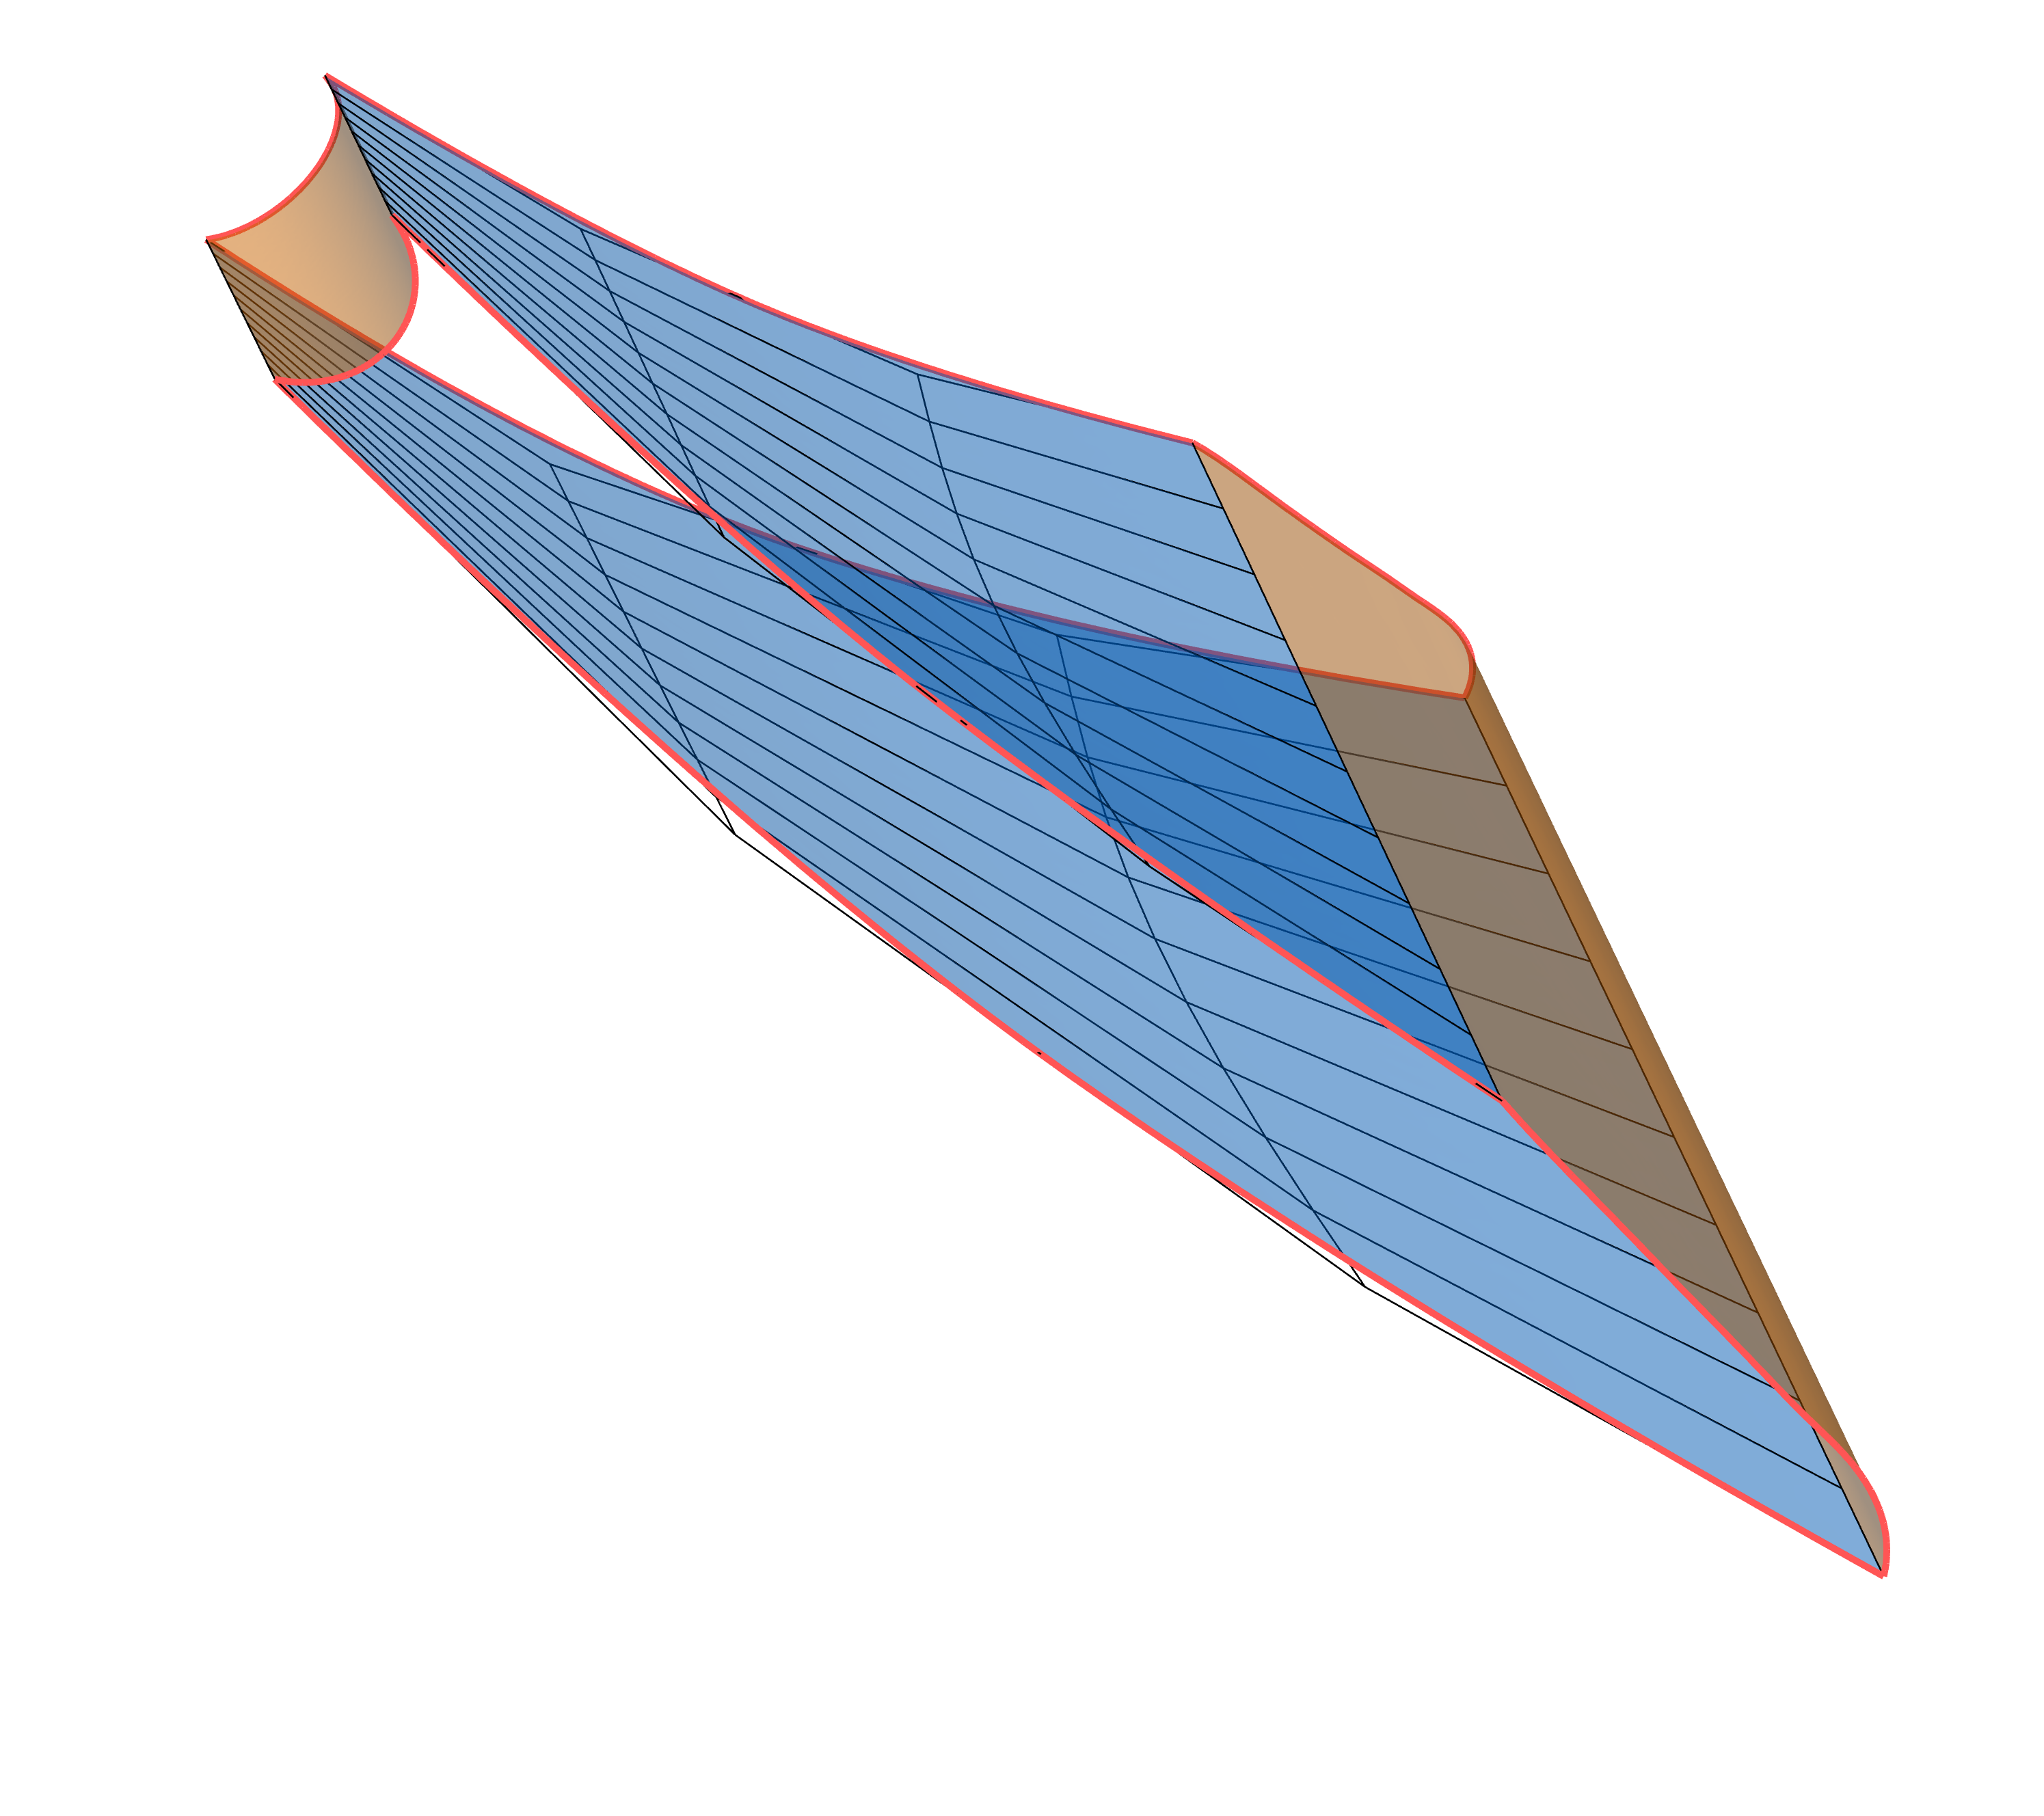
\includegraphics[width=0.4\textwidth]{../tec/slots/16.png}
		\caption{Connecting $I(u,v)$ and $O(u,v)$ yields the blue surfaces.}
		\label{fig:slot_connection}
	\end{figure}

	In the next step, we connect the boundary curves of $I(u,v)$ and $O(u,v)$. The suction-sided boundaries ($u = 0$) and the pressure-sided boundaries ($u = 1$) are connected by two NURBS surfaces. Given a value $v \in [0,1]$, we can construct two more equidistant intermediate control points for each $u \in \{0,1\}$. For this purpose, we define four input angles. The suction-sided inlet angle $\alpha_\textrm{suction}$, the pressure-sided inlet angle $\alpha_\textrm{pressure}$, the suction-sided outlet angle $\beta_\textrm{suction}$ and the pressure-sided outlet angle $\beta_\textrm{pressure}$. Figure \ref{fig:slot_connection} shows an example of this procedure, in which the connecting surfaces are blue.

	\begin{figure}[H]
		\centering
		\begin{subfigure}{.39\textwidth}
			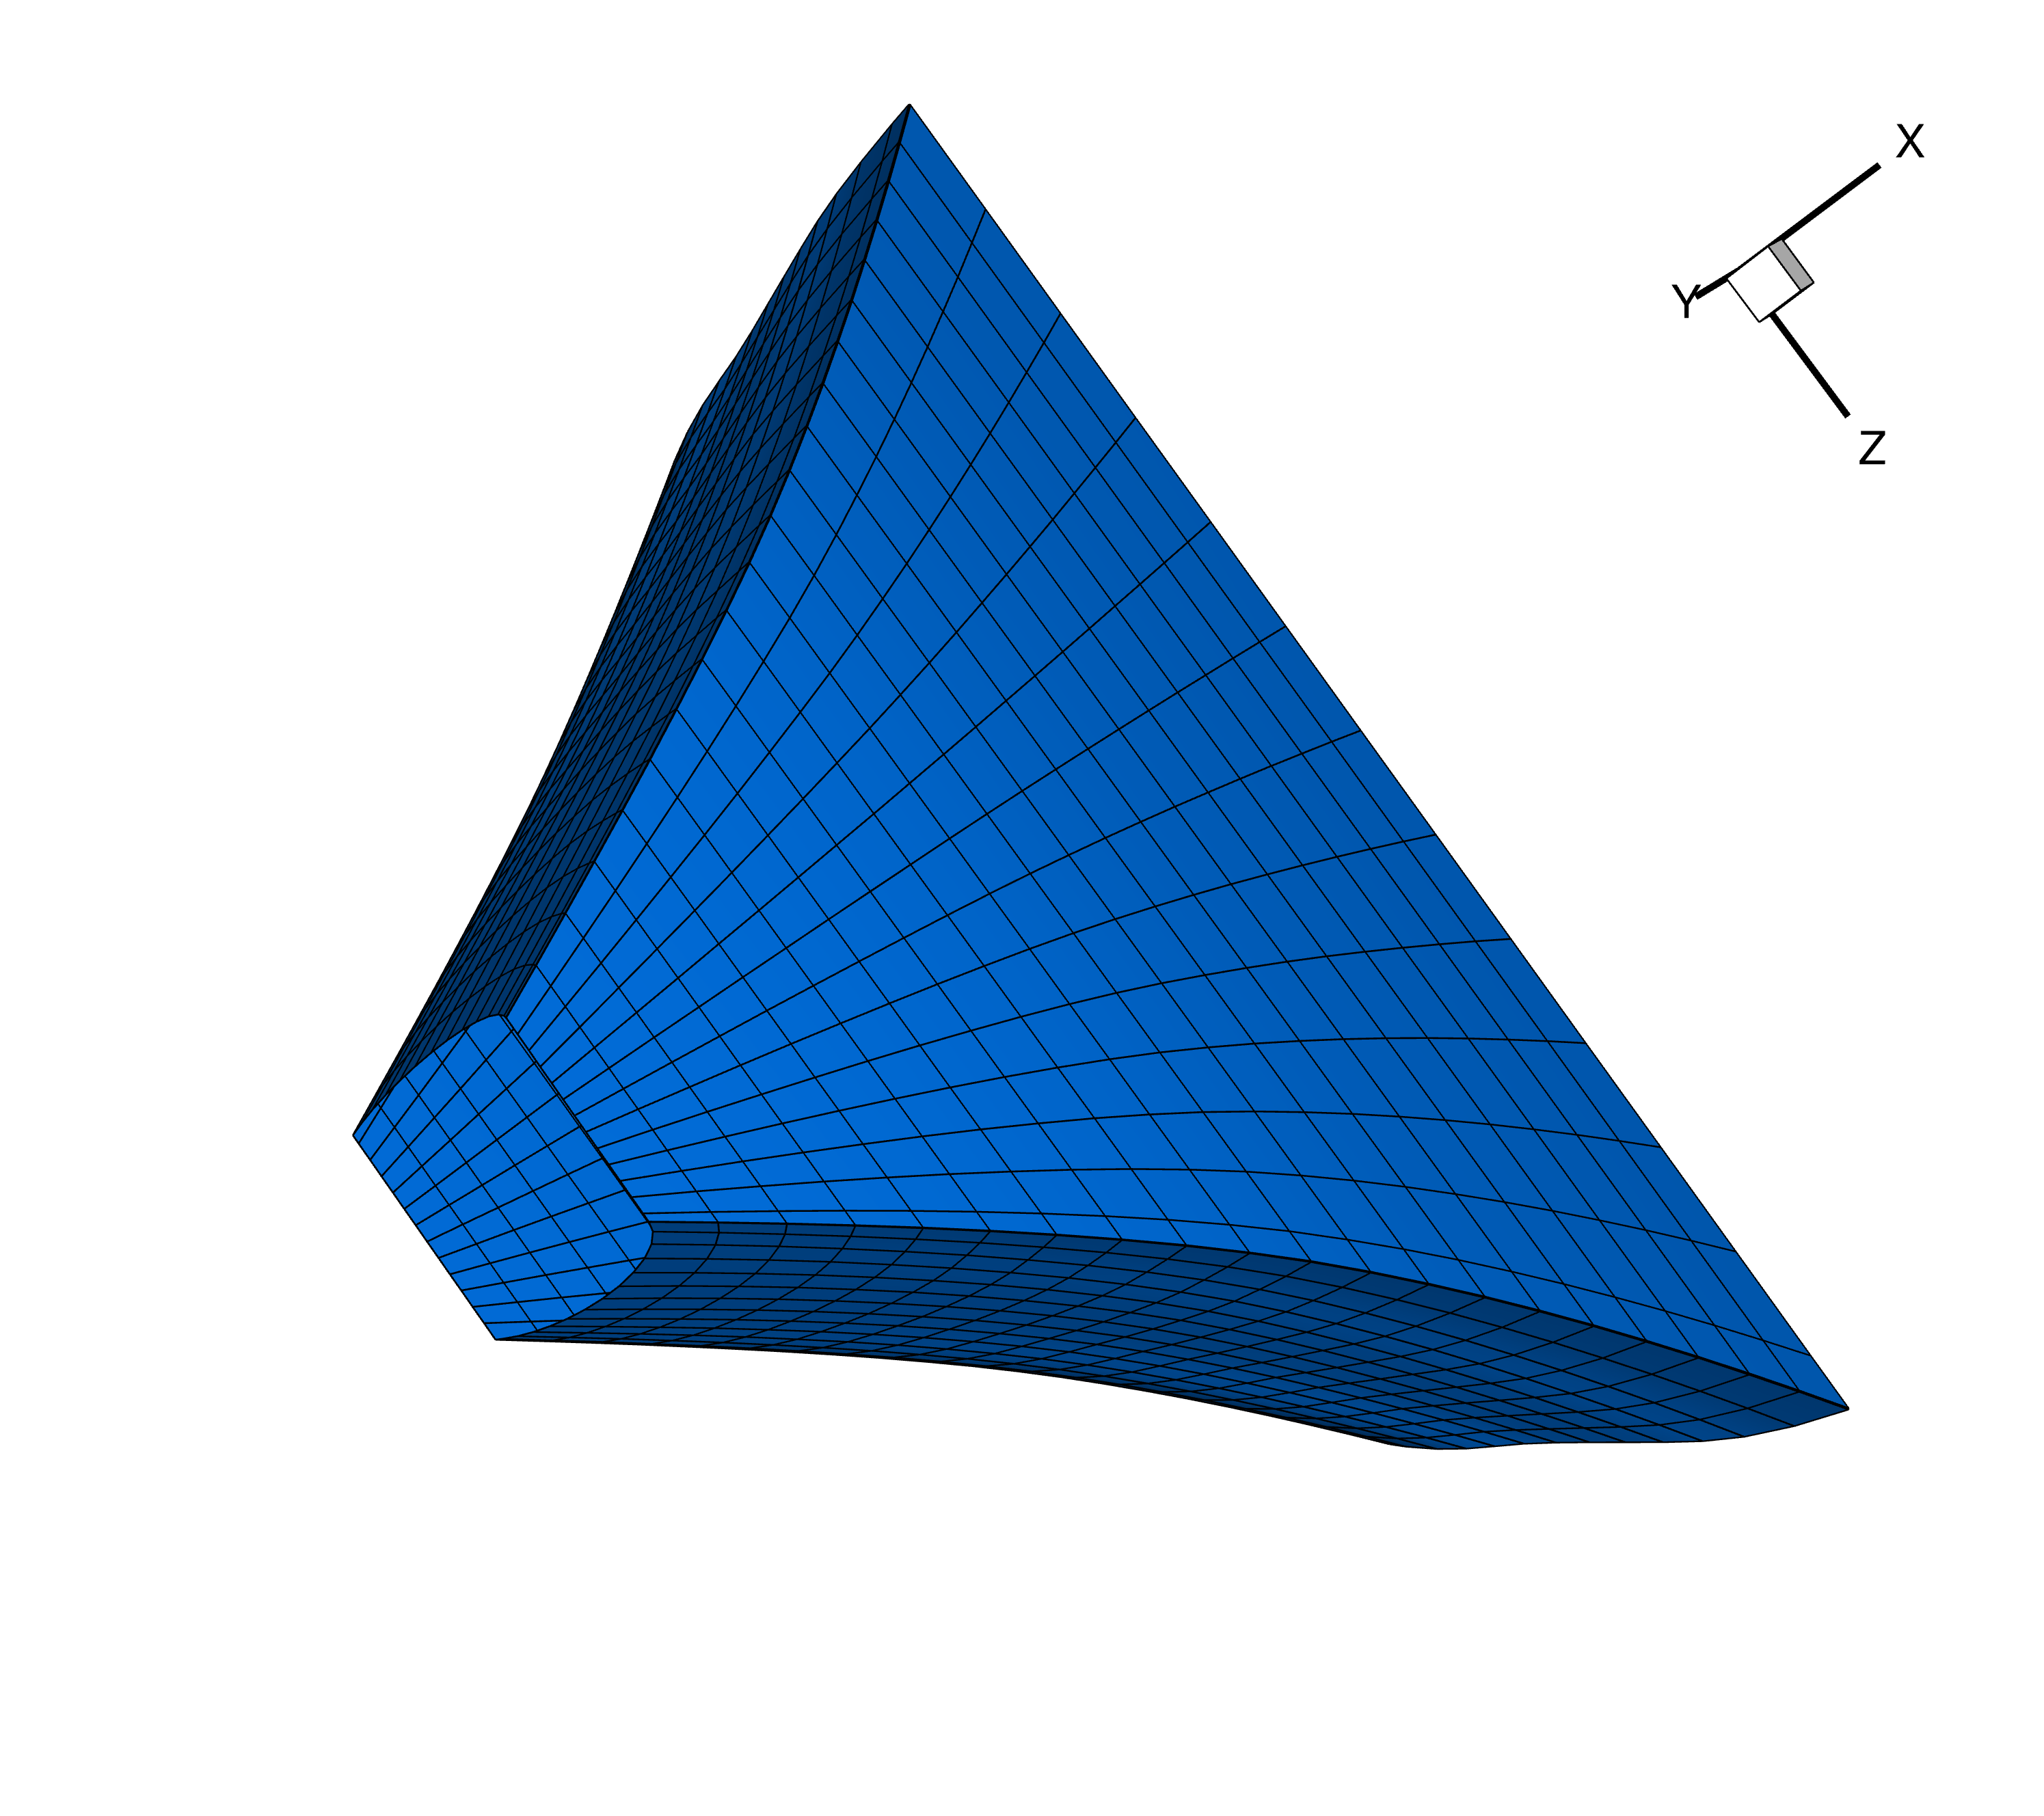
\includegraphics[width=\textwidth]{../tec/slots/17.png}
			\caption{Without fillets.}
		\end{subfigure}
		\begin{subfigure}{.39\textwidth}
			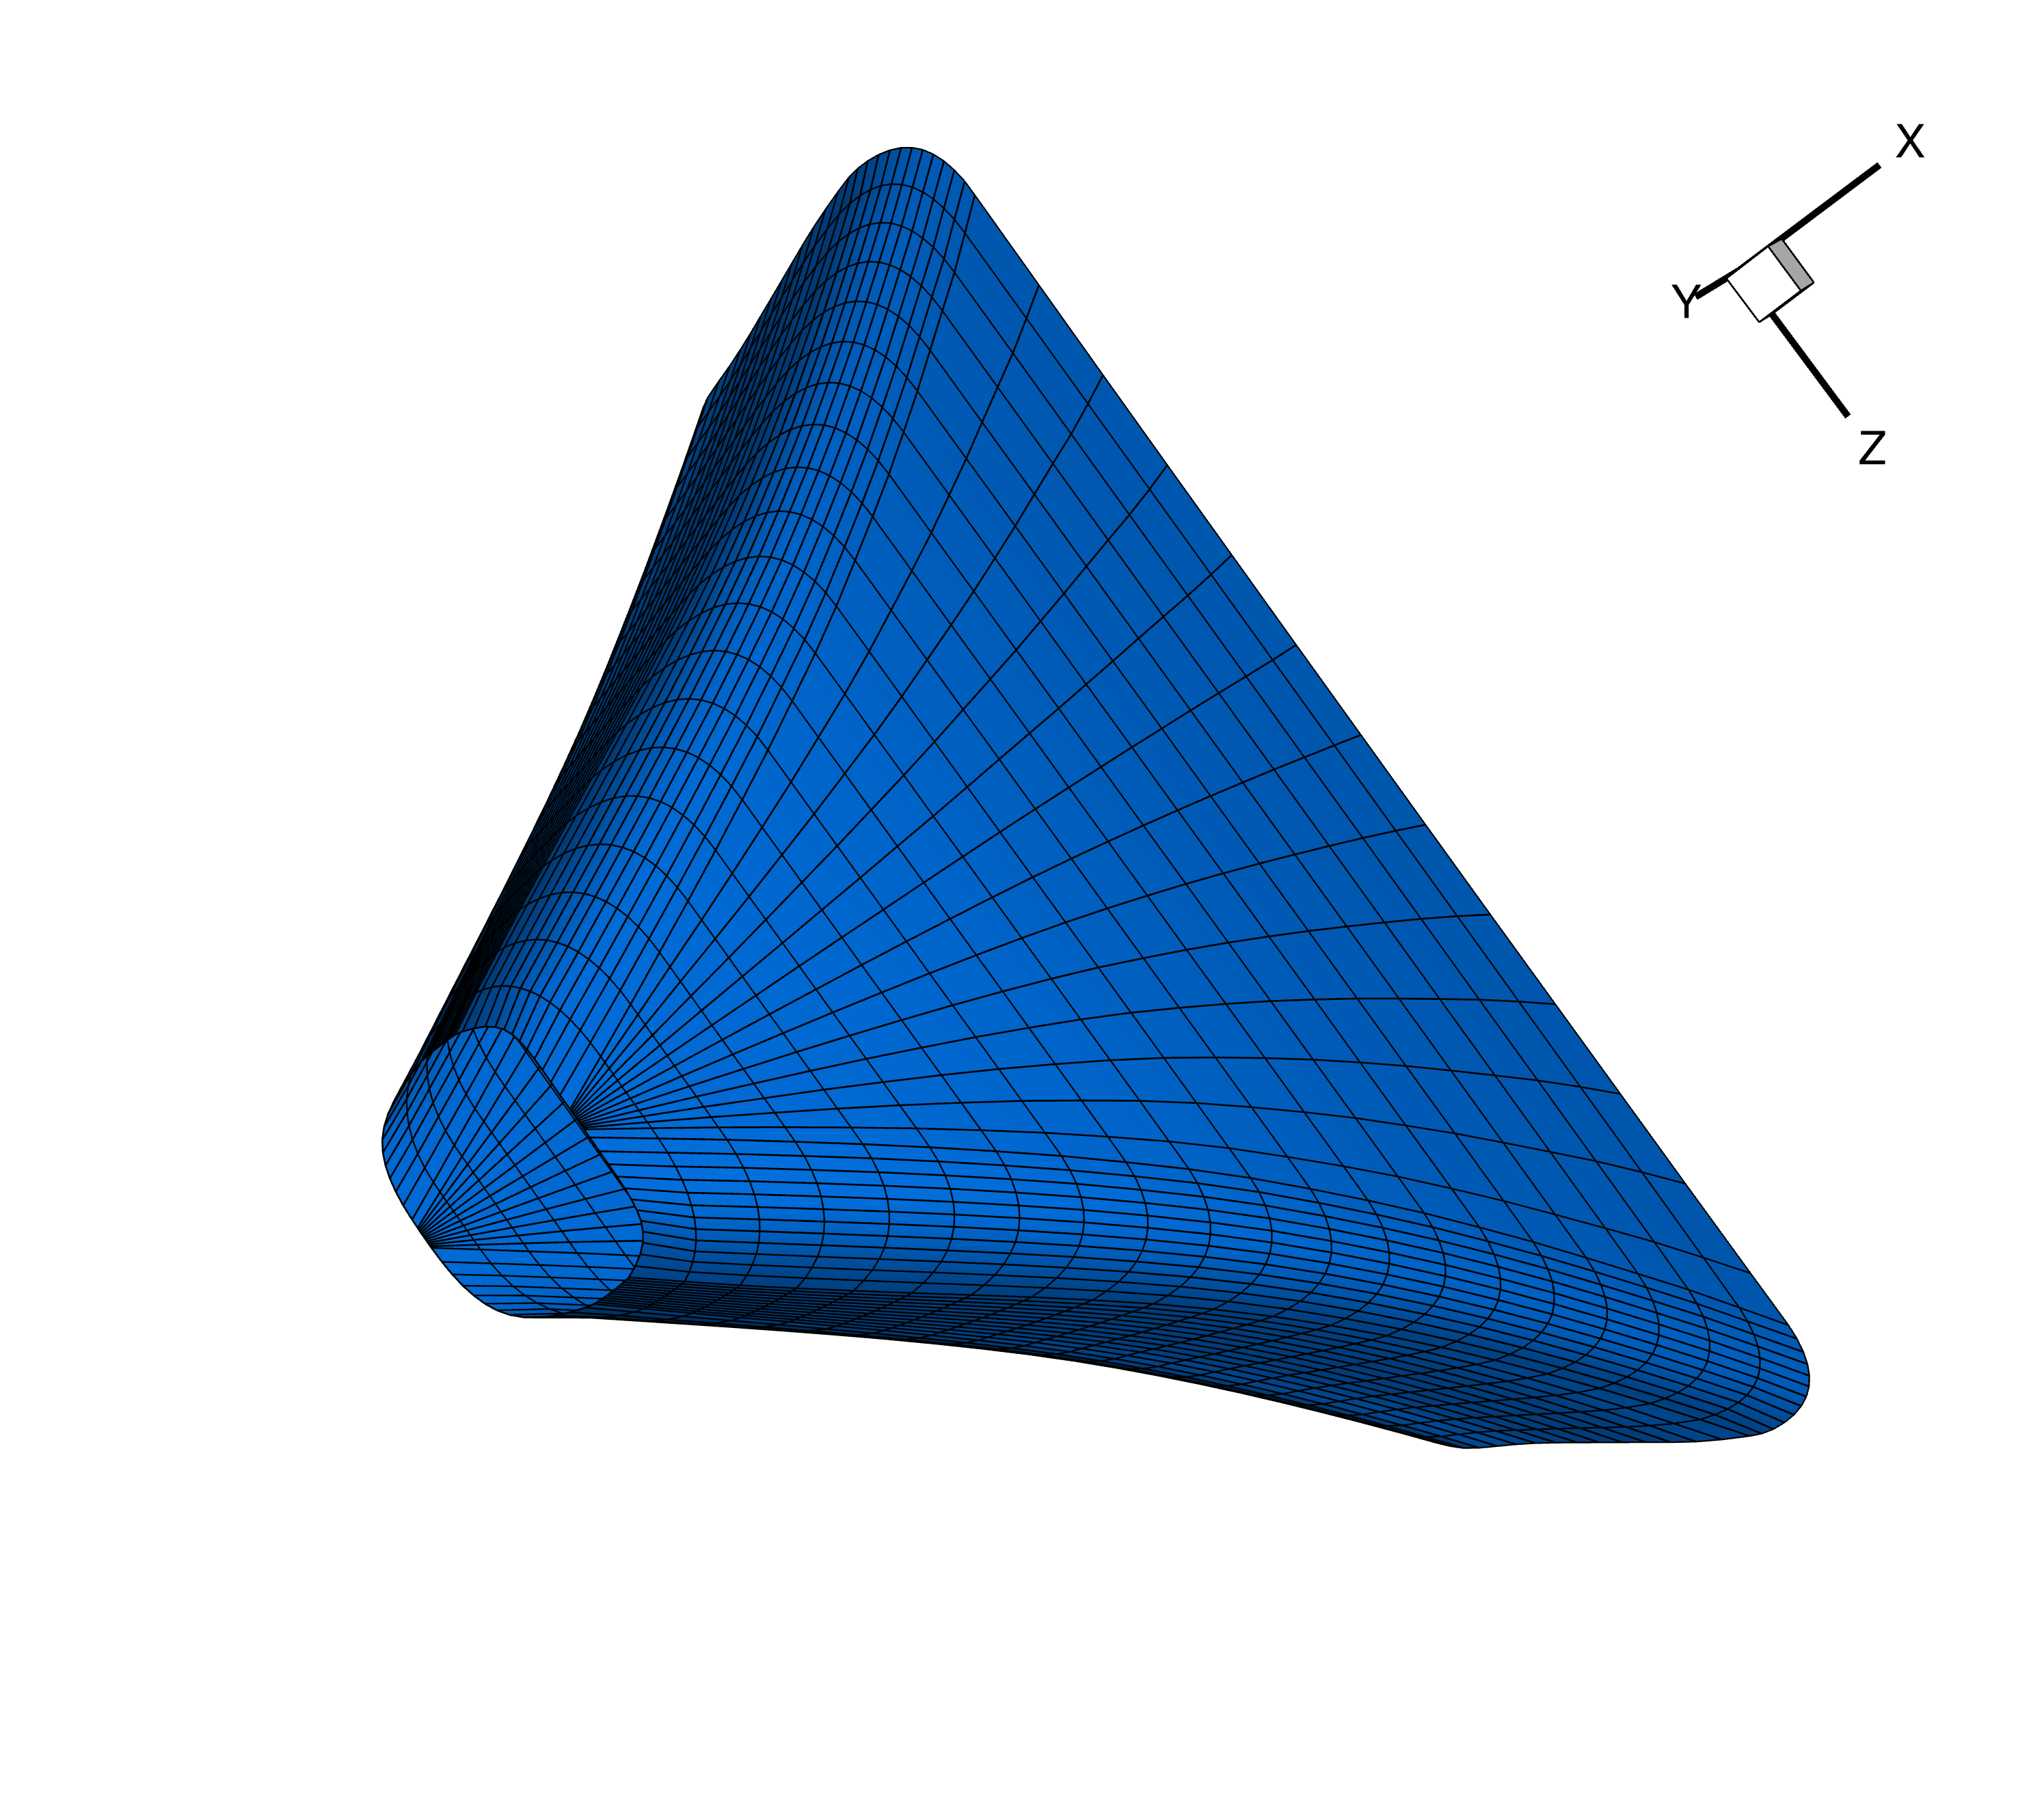
\includegraphics[width=\textwidth]{../tec/slots/18.png}
			\caption{With fillets.}
		\end{subfigure}
		\begin{subfigure}{.2\textwidth}
			\includesvg[width=\textwidth]{../python/rightAngleFillet}
			\vspace{1cm}
			\caption{Fillet creation.}
		\end{subfigure}
		\caption{Adding fillets to the slot surface.}
		\label{fig:slot_coon}
	\end{figure}

	The boundaries of the emerging surface, which are represented in red in Figure \ref{fig:slot_connection} are then connected using Coons patches. Combining the Coons patches of the two boundaries with the suction- and pressure-sided surfaces we created, we can make a slot surface like on the left side of Figure \ref{fig:slot_coon}.

	Next, we add fillets to the isoparameter curves of the slot curves. Since the isoparametric curves are not planar, we cannot use the methods from Section \ref{sec:filletcurves}. Instead, we use a different approach. We assume that the corners of the isoparameter curves are right-angled corners. In this case, we can use the fillet procedure shown in Figure \ref{fig:slot_coon}, where we trim the curves near the corner by the input radius $r$ and connect the trimmed curves using a circular arc, the midpoint of which is a mirror image of the corner.

	\begin{figure}[H]
		\centering
		\begin{subfigure}{.35\textwidth}
			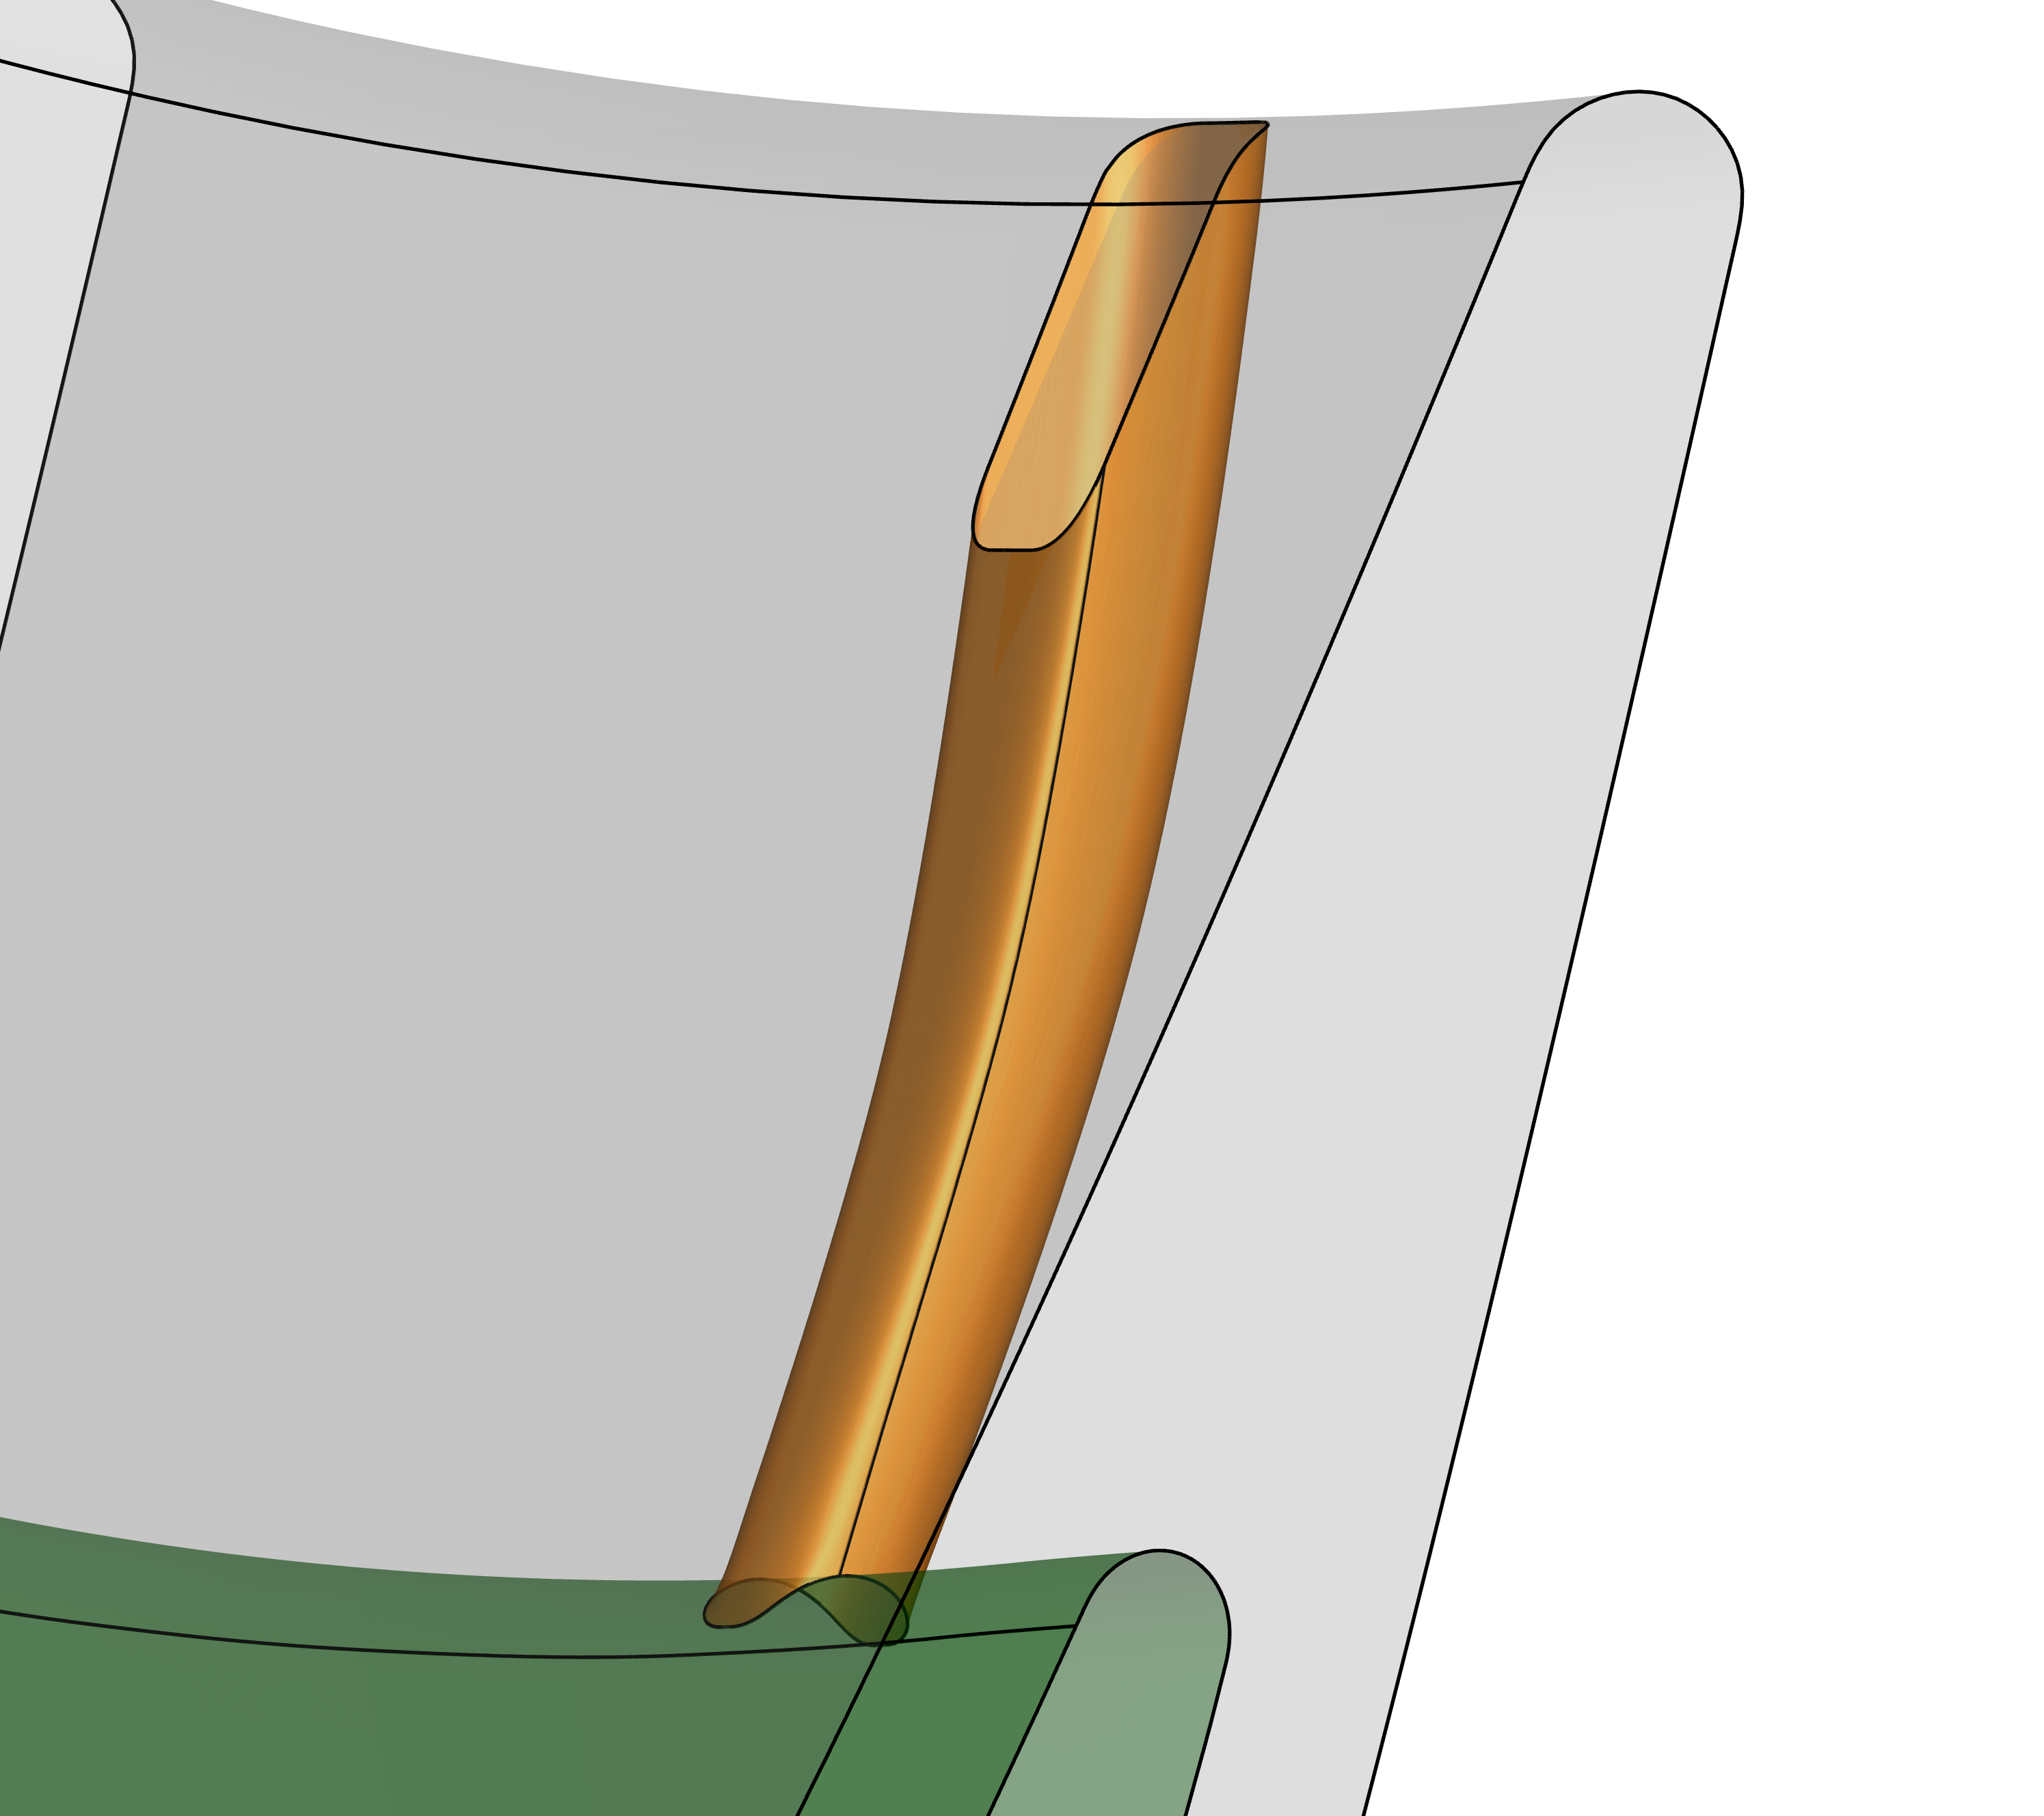
\includegraphics[width=\textwidth]{../tec/slots/12.png}
		\end{subfigure}
		\begin{subfigure}{.35\textwidth}
			\includegraphics[width=\textwidth]{../tec/slots/11.png}
		\end{subfigure}
		\caption{An array of slots constructed with realistic angles $\omega_L$ and $\omega_H$.}
		\label{fig:slots_real}
	\end{figure}

	The figures prior to Figure \ref{fig:slots_real} show relatively big angles $\omega_L$ and $\omega_H$ to better visualize the methods used for the construction. Although the presented angles produce valid slot surfaces, smaller angles are favorable in realistic scenarios. A more realistic setup can be seen in Figure \ref{fig:slots_real}.

\section{Implementation}\label{sec:implementation}
	The two blade setups that can be seen in Figure \ref{fig:results_complete} were generated in 40 seconds on a computer with 8 single-threaded cores, each of which have a clock rate of 4GHz. Alongside the mathematical procedures that were presented in Chapter \ref{chap:methods}, the performance of CoolingGen was achieved through OpenMP, which is a shared memory API that allows for parallel code execution. CoolingGen currently provides two different output formats: the Tecplot ASCII file format and the CENTAUR ASCII file format. Tecplot was used to create many of the blade/vane geometry surfaces and serves as a preview tool. To use CoolingGen's output surfaces in simulations, the CENTAUR output plays a large role.

\chapter{Discussion}
	CoolingGen proves to be a fast and accurate tool to model turbine blades and vanes. Using the CENTAUR file format, it is possible to combine the surfaces, put a FEM (finite element method) mesh onto the resulting surface and run a CFD (computational fluid dynamics) simulation on the FEM mesh.

	\section{Cooling Design Process Chain}
		\begin{figure}[H]
			\centering
			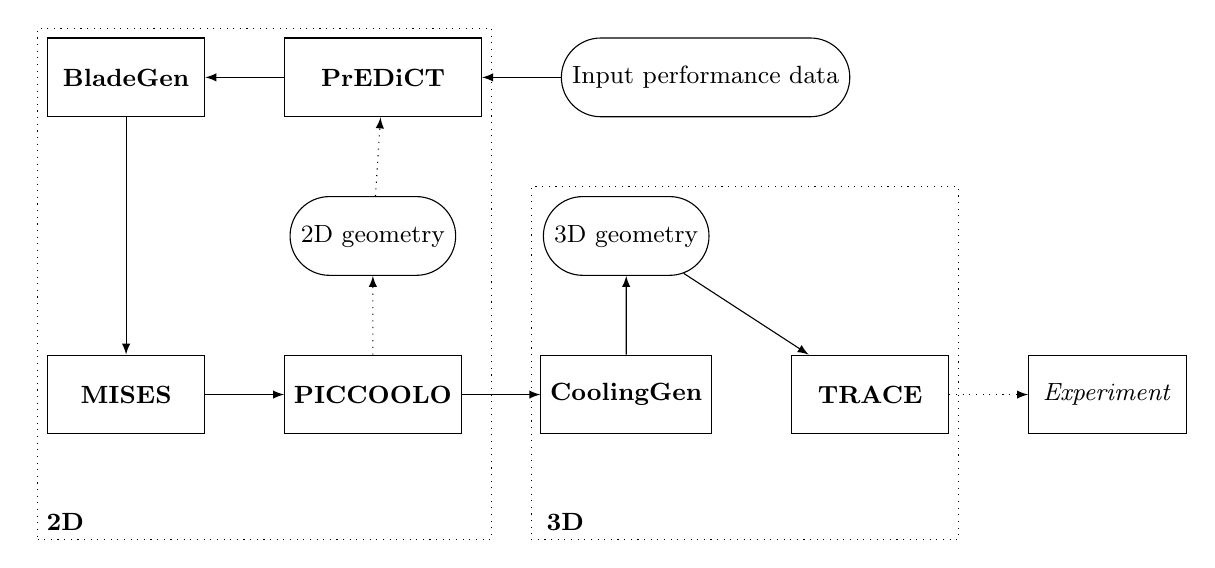
\begin{tikzpicture}[font=\small]
				\node[draw, rounded rectangle, minimum width=2cm, minimum height=1cm] (GTlab) 							{Input performance data};
				\node[draw, rectangle, minimum width=2.5cm, minimum height=1cm, left=of GTlab] (PrEDiCT) 				{\textbf{PrEDiCT}};
				\node[draw, rectangle, minimum width=2cm, minimum height=1cm, left=of PrEDiCT] (BladeGen)				{\textbf{BladeGen}};
				\node[minimum width=2.5cm, minimum height=1cm, below=of BladeGen] (spacer)								{};
				\node[draw, rectangle, minimum width=2cm, minimum height=1cm, below=of spacer] (MISES)					{\textbf{MISES}};
				\node[draw, rectangle, minimum width=2cm, minimum height=1cm, right=of MISES] (PICCOOLO)				{\textbf{PICCOOLO}};
				\node[draw, rounded rectangle, minimum width=2cm, minimum height=1cm, above=of PICCOOLO] (2DGeom)		{2D geometry};
				\node[draw, rectangle, minimum width=2cm, minimum height=1cm, right=of PICCOOLO] (CoolingGen)			{\textbf{CoolingGen}};
				\node[draw, rectangle, minimum width=2cm, minimum height=1cm, right=of CoolingGen] (TRACE)				{\textbf{TRACE}};
				\node[draw, rounded rectangle, minimum width=2cm, minimum height=1cm, above=of CoolingGen] (Geometry)	{3D geometry};
				\node[text width = 2cm, minimum height = 0.1cm, inner sep=0,outer sep=0, below=of MISES] (pad2D) 		{\textbf{2D}};
				\node[text width = 2cm, minimum height = 0.1cm, inner sep=0,outer sep=0, below=of CoolingGen] (pad3D) 	{\textbf{3D}};
				\node[draw, rectangle, minimum width=2cm, minimum height=1cm, right=of TRACE] (Experiment)				{\textit{Experiment}};

				\draw[-latex]
					(GTlab) edge (PrEDiCT)
					(PrEDiCT) edge (BladeGen)
					(BladeGen) edge (MISES)
					(MISES) edge (PICCOOLO)
					(PICCOOLO) edge (CoolingGen)
					(Geometry) edge (TRACE)
					(CoolingGen) edge (Geometry)
					(PICCOOLO) edge[dotted] (2DGeom)
					(TRACE) edge[dotted] (Experiment)
					(2DGeom) edge[dotted] (PrEDiCT);
				
				\node[draw,dotted,fit=(PrEDiCT) (BladeGen) (MISES) (PICCOOLO) (pad2D)] {};
				\node[draw,dotted,fit=(CoolingGen) (TRACE) (Geometry) (pad3D)] {};

			\end{tikzpicture}
			\caption{The cooling design process chain.}
			\label{fig:processchain}
		\end{figure}

		In order to design sensible cooling geometries, a multitude of tools are used at the DLR. First, a two-dimensional profile of the blade/vane is designed. To do this, we use the program PrEDiCT to determine the turbine geometry, flow conditions and the cooling requirements. We can then calculate the blade and vane geometries using BladeGen. MISES is a computational fluid dynamics (CFD) simulator, which we use to simulate air flow on a two-dimensional section of the resulting blade/vane-cascades. Using PICCOOLO, we can design and evaluate two-dimensional cooling geometry based on the simulated flow data. We can iteratively apply those tools to redetermine the cooling requirements on the updated blade/vane section and redesign the two-dimensional cooling geometries.

		In the future, three-dimensional cooling structures can be designed using CoolingGen using the findings of the previous two-dimensional iteration process. The input XML files for PICCOOLO and CoolingGen are quite similar, although CoolingGen does require more inputs. The resulting three-dimensional geometry can then be evaluated using a three-dimensional CFD simulator called TRACE. If a blade/vane model performs well enough, it can be manufactured and experiments can be performed with it. This cooling design process chain can also be seen in Figure \ref{fig:processchain}.

	\section{Desiderata \& Future Work}
		As previously mentioned, the output of CoolingGen consists only of a set of surfaces. However, these surfaces still have to be combined using the help of CENTAUR before creating a FEM mesh. Since CoolingGen (or any other DLR tool in the process chain previously presented) is currently not capable of surface trimming, the implementation of combined geometries remains a challenge that has to be considered in the future. Fortunately, the curves at which the surfaces need to be trimmed are known, as can be seen in Section \ref{sec:filmcooling} and Section \ref{sec:slots}. Given this kind of notion, it would then also be simple to define a full body made up by CoolingGen's output surfaces. Given any point in space, we could project it onto the combined surface and find the normal of the tangent plane of the combined surface at the projected point. The inner product of the projection path and the normal vector would then always be positive (negative) as long as the original point would lie inside (outside) the surface.

		A second shortcoming of the current version of CoolingGen certainly is the structure of the output geometries. Right now, the output surfaces are stored as ASCII point clouds. However, CENTAUR also accepts binary file formats in which NURBS surfaces can be specified using their knot vectors and control points. These file formats provide more accurate outputs (given that the surfaces were created using NURBS) given less file size, which is favorable for the creation of FEM meshes. This mode of operation would probably signficantly decrease the running time of CoolingGen.

		Lastly, even though CoolingGen currently supports all the geometries presented in Chapter \ref{chap:results}, there are still quite a few such geometries that are considered best practices in cooling design and yet are missing. These include but are not limited to turbulation ribs, pin-fin arrays and a second kind of impingement cooling, where neighboring cooling channels are connected through holes. The presented shapes of film cooling holes do certainly also not comprise the diversity of existing film cooling. These tasks require more time than was given for this thesis project.

% Bibliography, numbered and formatted like a chapter (for the TOC as well)
\printbibliography[heading=bibnumbered, title=References]

\end{document}